\documentclass[10pt, a4paper, twoside, openright, fleqn,%
               headinclude, footinclude, parskip=half,%
               numbers=noenddot, cleardoublepage=empty]{scrbook}

\usepackage[utf8]{inputenc} 
\usepackage{mathpazo} %-- use Palatino font
\usepackage[left=25mm, top=25mm]{geometry}
\usepackage{amsmath, amssymb, amsthm}
\usepackage[square]{natbib}
\usepackage{subcaption}
\usepackage{xspace}
\usepackage[breaklinks=true,
            colorlinks=true,
            linktocpage=true,
            allcolors=colorforlinks]{hyperref} 
\usepackage[ruled, vlined, algochapter, linesnumbered]{algorithm2e}
\usepackage{calc}
\usepackage{ccicons}
\usepackage{xspace}
\usepackage{longtable}
\usepackage{booktabs}
\usepackage[english]{babel} 
\usepackage{listings}
\usepackage{scrhack} % ignore warnings about deprecated KOMA-Script
\usepackage[printonlyused, smaller, withpage]{acronym}
\usepackage[usenames, dvipsnames]{xcolor}
\usepackage{graphicx}
\usepackage{pdfpages}
\usepackage{wrapfig}
\usepackage[format=plain, font=small,labelfont=bf]{caption}
\usepackage{url}
\usepackage{chngcntr}
\usepackage{multicol}

\makeatletter
\renewenvironment{thebibliography}[1]{%
   \section*{\refname \@mkboth{\MakeUppercase\refname}{\MakeUppercase\refname}}%
   \begin{multicols}{2}
   \list{\@biblabel{\@arabic\c@enumiv}}{%
     \settowidth\labelwidth{\@biblabel{#1}}%
     \leftmargin\labelwidth
     \advance\leftmargin\labelsep
     \@openbib@code
     \usecounter{enumiv}%
     \let\p@enumiv\@empty
     \renewcommand\theenumiv{\@arabic\c@enumiv}}%
     \sloppy
     \clubpenalty4000
     \@clubpenalty \clubpenalty
     \widowpenalty4000%
     \sfcode`\.\@m}
{
   \def\@noitemerr{\@latex@warning{Empty `thebibliography' environment}}%
   \endlist\end{multicols}
}
\makeatother

\NewDocumentCommand{\codeword}{v}{%
    \texttt{\textcolor{black}{#1}}%
}
\lstset{language=C,keywordstyle={\bfseries \color{blue}}}



\newcommand{\myName}{Céline Dion}
\newcommand{\myTitle}{The optimal Delaunay triangulation of cheesy songs}

\newcommand{\myGroup}{3D geoinformation group}
\def\myGroupLogo{figs/tud-3dgeoinfo-black.png}
\newcommand{\myDepartment}{Department of Urbanism}
\newcommand{\myFaculty}{Faculty of the Built Environment \& Architecture}
\newcommand{\myUni}{Delft University of Technology}

% \newcommand{\myGroup}{Geo-Database Management Centre}
% \def\myGroupLogo{figs/GDMC-LOGO12.jpg}
% \newcommand{\myDepartment}{Department of the OTB}
% \newcommand{\myFaculty}{Faculty of Architecture \& the Built Environment}
% \newcommand{\myUni}{Delft University of Technology}

\newcommand{\myGraduationYear}{2020}
\newcommand{\myGraduationMonth}{February}

\newcommand{\mySupervisorOne}{Prof.dr.\ Jan Smit}
\newcommand{\mySupervisorTwo}{Dr.\ Gerard Joling}
\newcommand{\myCoreader}{ir.\ Gordon Heuckeroth}


%-- for names for \autoref commands
\def\chapterautorefname{Chapter}
\def\sectionautorefname{Section}
\def\subsectionautorefname{Section}
\def\subsubsectionautorefname{Section}
\def\algorithmautorefname{Algorithm}
 
%-- for pdf metadata
\hypersetup{pdfauthor={\myName}}
\hypersetup{pdfkeywords={thesis, geomatics, TU Delft}}
\hypersetup{pdfsubject={A thesis submitted to the Delft University of Technology in partial fulfillment of the requirements for the degree of Master of Science in Geomatics}}
\hypersetup{pdftitle={\myTitle}}

%-- handy shortcuts
\newcommand{\ie}{i.e.}
\newcommand{\eg}{e.g.}

%-- colours for the hyperlinks
\definecolor{colorforlinks}{RGB}{27, 60, 131}




\setcapindent{1em} %-- for captions of Figures
% \setcounter{tocdepth}{\sectiontocdepth}

\subject{MSc thesis in Geomatics}
\title{\myTitle}
\author{\myName}
\date{\myGraduationMonth\xspace\myGraduationYear}
\publishers{A thesis submitted to the Delft University of Technology in partial fulfillment of the requirements for the degree of Master of Science in Geomatics}

\begin{document}

%******************************************************************
% Frontmatter
%******************************************************************
\frontmatter


\includepdf{cover/cover_front.pdf}
\cleardoublepage

\maketitle[3]

%!TEX root = ../thesis.tex

\thispagestyle{empty}

\hfill
\vfill

\noindent\myName: \textit{\myTitle} (\myGraduationYear)\\
\ccby\xspace This work is licensed under a Creative Commons Attribution 4.0 International License. To view a copy of this license, visit \url{http://creativecommons.org/licenses/by/4.0/}.

\vspace{3em}
\vspace{3em}

\noindent{} The work in this thesis was carried out in the:\\

\begin{tabular}{ll}
\parbox{0.3\textwidth}{\includegraphics[width=\linewidth]{\myGroupLogo}}
&
\parbox{0.7\textwidth}
{
  \myGroup\\
  \myDepartment\\
  \myFaculty\\
  \myUni\\
}       
\end{tabular}

\vspace{3em}
\noindent
\begin{tabular}{ll}
Supervisors:  &  \mySupervisorOne \\
              &  \mySupervisorTwo \\
\end{tabular}
\cleardoublepage

\chapter*{Abstract}


\emph{[Should fit on one page.]}

Bacon ipsum dolour sit amet porchetta beef turkey, bacon turducken boudin hamburger venison ball tip. Brisket pork loin bresaola short loin ground round leberkas pastrami tongue jerky cow turducken beef ribs. Pork ribeye landjaeger prosciutto pig venison tenderloin. Swine beef ribs kielbasa, porchetta tenderloin salami venison pork belly tail.
Bacon ipsum dolour sit amet porchetta beef turkey, bacon turducken boudin hamburger venison ball tip. Brisket pork loin bresaola short loin ground round leberkas pastrami tongue jerky cow turducken beef ribs. Pork ribeye landjaeger prosciutto pig venison tenderloin. Swine beef ribs kielbasa, porchetta tenderloin salami venison pork belly tail.
Bacon ipsum dolour sit amet porchetta beef turkey, bacon turducken boudin hamburger venison ball tip. Brisket pork loin bresaola short loin ground round leberkas pastrami tongue jerky cow turducken beef ribs. Pork ribeye landjaeger prosciutto pig venison tenderloin. Swine beef ribs kielbasa, porchetta tenderloin salami venison pork belly tail.

\clearpage
\setcounter{tocdepth}{2}

\tableofcontents
\listoffigures
\listoftables
\listofalgorithms
\clearpage
\chapter*{Acronyms}

\begin{acronym}[UML]
  \acro{dtm}[DTM]{digital terrain model}
  \acro{dsm}[DSM]{digital surface model}
  \acro{gis}[GIS]{geographical information system}
  \acro{gnss}[GNSS]{global navigation satellite system}
  \acro{ins}[INS]{inertial navigation system}
  \acro{imu}[IMU]{inertial measurement unit}
  \acro{gui}[GUI]{graphical user interface}
  \acro{dt}[DT]{Delaunay triangulation}
  \acro{cdt}[CDT]{constrained Delaunay triangulation}
  \acro{tin}[TIN]{triangular irregular network}
  \acro{ndw}[NDW]{Nationaal Dataportaal Wegverkeer}
  \acro{rws}[RWS]{Rijkswaterstaat}
  \acro{rhdhv}[RHDHV]{Royal HaskoningDHV}
  \acro{mle}[MLE]{maximum likelihood estimation}
  \acro{rmse}[RMSE]{root mean squared error}
  \acro{als}[ALS]{airborne laser scanning}
  \acro{mls}[MLS]{mobile laser scanning}
  \acro{nwb}[NWB]{Nationaal Wegenbestand}
  \acro{ahn}[AHN]{Actueel Hoogtebestand Nederland}
  \acro{ahn2}[AHN2]{Actueel Hoogtebestand Nederland 2}
  \acro{ahn3}[AHN3]{Actueel Hoogtebestand Nederland 3}
  \acro{ahn3}[AHN3]{Actueel Hoogtebestand Nederland 3}
  \acro{dtb}[DTB]{Digitaal Topografisch Bestand}
  \acro{bgt}[BGT]{Basisregistratie Grootschalige Topografie}
  \acro{ransac}[RANSAC]{random sample consensus}
  \acro{pcd}[PCD]{phase coded disk}
  \acro{idw}[IDW]{inverse distance weighting}
  \acro{nbrs}[NBRS]{non-branching road segment(s)}
  \acro{jte_id}[JTE ID]{\textit{junctie} (intersection) ID number}
  \acro{r_roads}[R-roads]{Rijkswegen (motorways)}
  \acro{p_roads}[P-roads]{Provinciewegen (provincial roads)}
  \acro{g_roads}[G-roads]{Gemeentewegen (municipal roads)}
  \acro{w_roads}[W-roads]{\ac{rws}-managed roads}
\end{acronym}
\cleardoublepage

%******************************************************************
% Mainmatter
%******************************************************************
\mainmatter

%!TEX root = ../thesis.tex

\chapter{Introduction}
\label{chap:i}

\section{Motivation}
\label{sec:motivation}

Constructing and maintaining an up-to-date graph-like road network on the national level has a range of firmly established uses. Owing to its structure, it can be used efficiently for modelling and simulation purposes, such as traffic flow simulations, passenger transport modelling, construction and upgrade impact modelling (to pinpoint optimal locations and types of investment), and traffic noise load modelling (\cite{bell_lida_1997, zhu_li_2007, zhang_2011, duran_santos_2014, peng_etal_2020}). It can also be used for navigation; a graph-like road network representation is at the heart of most road navigation services (\cite{yue_etal_2008}). Combined with other data sets, we can mention an even wider range of use cases: complemented by ecological statistics and models, it can offer insight into the impact of the presence of roads, and planned road construction on the flora and fauna in their vicinity.

Or to mention a different type of example, an accredited model representing the road network in a digital format may be used as a shared working space when aggregating geospatial data relating to road infrastructure from various sources. It makes it possible for geographical road locations, topographical relationships, and arbitrary semantic information to reside in the same network-type data model, making analysis techniques more straightforward, enforcing consistency and saving effort for data providers who would otherwise all need to maintain their own road model (\cite{ekpenyong_etal_2007}). This example is closely related to the ambitions the provider of the Dutch digital road network, which is the primary subject of this research, has with their road network model.

One may remark that a two-dimensional representation with \textit{approximate} geographical locations may suffice for many of the purposes I listed as examples above, topology being the main concern in network analysis. For instance, \ac{gnss} navigation software often use snapping methods to ensure that the navigating vehicle always traverses the road graph – ensuring that even for imperfect positioning results navigation remains continuous (\cite{fouque_bonnifait_2008, chen_hsu_2020}). Traffic flow simulations are primarily concerned with traffic loads, road properties, and how roads are subdivided by intersections among other aspects. \textit{Mostly}, they are not concerned with the exact geographical locations of roads – as long as the topology is relatively accurate, any geographical permutation of the network will yield largely invariant results (\cite{thomson_richardson_1995}).

However, some applications are concerned with the road network in the context of its surroundings, which makes the accuracy of its georeferencing important. Noise modelling is such an application, because modelling the propagation of road noise concerns deriving the noise load affecting various objects in the vicinity of the the roads. This also involves considering objects that may impact the propagation of the noise, such as noise barriers, terrain, and buildings (\cite{ishiyama_etal_1991, bennett_1997, guarnaccia_quartieri_2012}).

A realistic noise propagation model should take into account terrain, and the 3D geometry of the surrounding objects. It should also take into account the position of roads \textit{relative to the terrain}. For instance, consider a hill with a building on one side and a road on the other, as shown in Figure \ref{fig:justification_illu}. The hill (the terrain) in this case acts as a noise barrier affecting the noise load received by the building. Unless the assumption holds that roads are always found \textit{on} the terrain, this is not yet enough information to derive the noise load. The assumption does not always hold because roads may be elevated, sunken into the ground, or built in tunnels. For instance, if the road in my example is built on a bridge with a similar height as the hill, then the hill will suppress the road noise much less effectively, and "snapping" the road to the terrain by ignoring its elevation would yield incorrect noise modelling results. One way to handle such scenarios is to take into account the absolute elevation of the road surfaces, in other words to use a 3D road network.

\begin{figure}
    \centering
    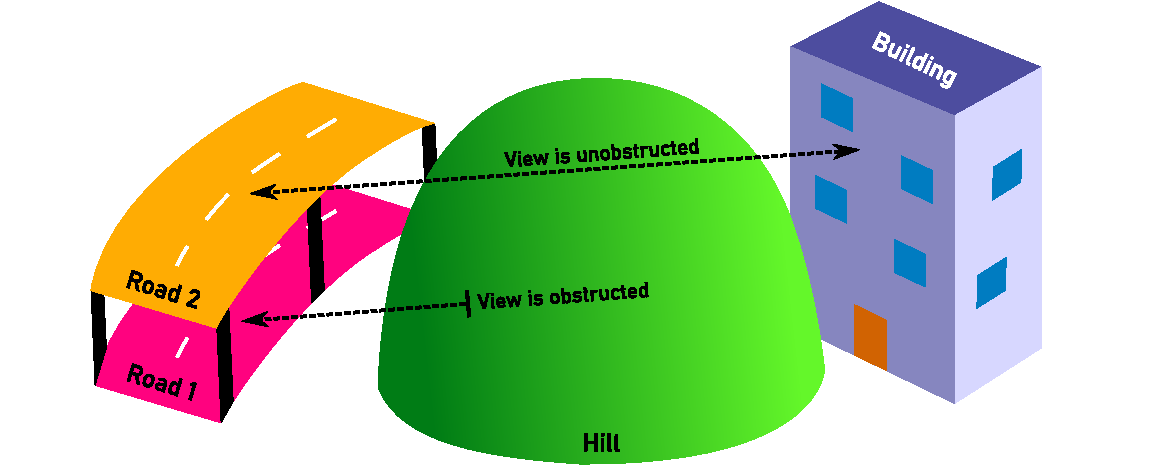
\includegraphics[width=\linewidth]{final_report/figs/justification_illu.pdf}
    \caption[Illustration of the 3D conversion justification]{This illustration shows a justification of the 3D conversion of NWB. Assuming that the road network always lies on the terrain (pink road) allows one to model the propagation of noise with the surrounding terrain and 3D objects taken into account. However, roads above or below the terrain elevation will be represented incorrectly. For instance, the noise from the true location of the road (yellow elevated road) reaches the building. "Snapping" it to the terrain suggests incorrectly that the hill blocks the noise.}
    \label{fig:justification_illu}
\end{figure}

2D-projected digital road models with mediocre accuracy have attracted great scientific and commercial attention since the advent of digital cartography and satellite navigation (\cite{taylor_etal_2001, fouque_bonnifait_2008, yue_etal_2008, chen_hsu_2020}). However, \textit{accurate 3D representations} are still atypical, owing to factors such as increased cost of generation and maintenance, increased complexity of visualisation and analysis, and a lack of significant use cases (\cite{zhu_li_2007, wang_etal_2014}). As a result, 2D road models are common in terms of both public and private geospatial providers, whereas accurate 3D road models are rare in comparison.

When a use case arises and an accurate 3D model is needed, providers generally have two options: to produce a new model, or to enrich an existing 2D model with elevation data. The decision generally depends on the quality of the available 2D data set relative to the requirements for the 3D model, as well as that of the dataset(s) available as sources of elevation data, with which the 2D model can be enriched, among other factors (\cite{zhu_li_2007, zhu_li_2008, wang_etal_2014}). In terms of the source of elevation data, the rule of thumb in the geospatial field is that data acquisition is far more expensive than re-using existing datasets, especially openly available ones. As a result, many providers first attempt to find a way to convert their datasets into 3D using existing data in such a cost-effective manner.

\section{The NDW commission}
\label{sec:commission}

In certain projects the accuracy requirement and restrictions on the modelling procedure may be prescribed legally. Such is the case for the client of the present dissertation research, the \ac{ndw} (National Road Traffic Data Portal), part of \ac{rws} (Directorate-General for Public Works and Water Management), a Dutch government organisation who are in the process of enriching their pre-existing open data 2D road model, called \ac{nwb} (National Road Database), with 3D data, to attain compliance with the new version of the Dutch noise legislation or \textit{geluidwetgeving}, coming into effect on the 1\textsuperscript{st} of January 2022. The new version of the legislation prescribes, among other things, a horizontal \textit{and vertical} accuracy of 20 centimetres for the road model underlying the noise simulations. Due to cost considerations and reasons related to \ac{ndw}’s data acquisition pipeline, the pre-existing 2D version of \ac{nwb} will be converted into a 3D dataset (dubbed \textit{3D-NWB}) primarily using open data geospatial datasets. They have produced a prototype implementation themselves, and subsequently contracted the consultant firm \ac{rhdhv} to create a commercial implementation based on their experience with the prototype. The development of this tool was concluded in December 2020, with a preliminary version of the results already publicly available on their website in addition to the traditional 2D version.

Thus for \ac{ndw}, the next year will be about assessing the quality of their new product and improving it as they see necessary. In particular, they wish to assess how it fares in terms of the requirements set by the law. This dissertation research attempts to contribute to this assessment by presenting an original system design and implementation that favours scientific correctness, and in which output accuracy can be qualitatively and quantitatively examined. By comparing the results of this academic implementation to that of the commercial one, it becomes possible to indirectly evaluate the commercial results' general quality and accuracy in an indirect manner. My work also explores various related geomatics topics in the process, which I specifically refer to as the academic aims of this project, in the present report.

My research was carried out in consultation with the above parties. In fact, the stages leading up to the submission of my dissertation proposal involved continuous consultation with personnel both at \ac{ndw} and \ac{rhdhv} while the commercial implementation was still being developed, to ensure that my research fits well with \ac{ndw}'s plans and the commercial implementation - in addition to answering various questions inspired purely by academic interest.

\section{Field and relevance}
\label{sec:relevance}

For reasons that will later become clear (see Section \ref{sec:input}), I primarily focused on a Lidar point cloud and a 3D topographical line dataset as elevation sources. In both of these datasets, it is clearly evidenced that roads are occasionally in complex three-dimensional relationships with one another and with their environment. For instance, they cross above and below other roads and are also frequently occluded by other objects such as vegetation and buildings. Already in the planning phase of the project the question had arisen, how such real-world geometries should be dealt with in the conversion process - evidently they will require special treatment relative to well-exposed road surfaces. The answer to this question is closely linked with which field of geoscience my project is positioned in.

The likely candidates in the context of digital road network modelling are \ac{gis} and geomatics. It is thus worth discussing briefly how each typically treats 3D objects. One of the reasons why 2D road models are popular is that their geometry and network properties can be analysed using a multitude of well-proven \ac{gis} methods and software kits. However, in \ac{gis} models, even if elevation measurements exist, they are generally only present as an \textit{elevation attribute} (i.e. a semantic data field, like street names), because \ac{gis} geometrical models do not typically support true 3D operations. This is conceptually identical to projecting the geometries onto the horizontal plane. Geometric models that treat the vertical dimension explicitly are more common in geomatics; namely 2.5D and 3D models. While using 2.5D models restricts the types of physical entities that can be modelled, it also greatly simplifies certain types of analysis conceptually and computationally. This makes it ideal for working on similar scales to \ac{gis}; on the national scale for instance, as in this research.

While 2.5D modelling initially appears to be a good candidate for this project, we may observe that it is by definition unsuitable for handling the 3D relationships that roads have with each other and with their environment. However, much like how the concept of divide-and-conquer works in computer science, it is also possible decompose three-dimensional, geometrical problems into smaller sub-problems until they become natively compatible with 2.5D methods which are simpler to solve individually than the 3D problem as a whole. This research is positioned in the field of geomatics because my system design is specifically intended to explore how 2.5D methods can be applied in a way that enables the \textit{piecewise} modelling of a national road network. The divide-and-conqer concept will be applied to decompose the road network into segments that can be individually, locally regarded as \textit{terrain} (i.e. a mathematical surface) and hence be modelled in 2.5D.

Geomatics is comprised of a wide range of disciplines, several of which are relevant to the present research. As it focuses on 2.5D methods to a great extent, it overlaps with the geomatics field of \textit{digital terrain modelling} in terms of how it generates and stores the digital representation of road surfaces, and as a consequence, the manner in which it will derive elevations from them: using \textit{spatial interpolation}. As the overview of the methods in Section \ref{sec:methodsoverview} reveals, it also strongly overlaps with the geomatics discipline of \textit{feature extraction} (and to a lesser extent, \textit{photogrammetry}), because of the intermediate steps used by the pipeline to derive the 2.5D road surface models from our input datasets.

This is in line with my goal to study how a combination of mainly geomatics-based tools and methods can be used to accomplish the tasks required by \ac{ndw}, and to also assess their accuracy and suitability when used in this way. However, I also use \ac{gis} methods "under the hood" in all parts of the project - for instance, 2D geometry intersection tests, orientation tests and spatial queries are pervasive in the implementation, and are thus often mentioned in the detailed description of the processing steps found in Section \ref{sec:methods}. Furthermore, my research often touches on mathematics and statistics, for instance I use polynomial fitting and maximum likelihood estimation (\ac{mle}) throughout the implementation (as examples of the former) and metrics such as standard deviation and \ac{rmse} (as examples of the latter).

\section{Research questions}
\label{sec:rq}

My main research question is \textit{"How can we achieve a 3D conversion of the \ac{nwb} dataset using Dutch open geospatial data and a primarily 2.5D-based surface modelling methodology, while guaranteeing optimal and quantifiable accuracy and completeness?"}. It was distilled from the main areas of interest that we settled on during the preparatory stages of the project, while planning the project with my academic mentors, as well as \ac{ndw} and \ac{rhdhv}. The question is comprised of two halves, which I initially intended to devote equal amounts of attention to - the question of devising a system design and implementing it, and that of assessing its effectiveness and the accuracy and completeness of the output it generates (as well as comparing it with the commercial results).

I eventually settled on focusing more time and effort on the system design and integration (i.e. \textit{performing} the elevation-enrichment of NWB), both because it required more time than initially anticipated, and because the quality and accuracy assessment of the results (and their comparison with the commercial results) was more straightforward than expected. Furthermore, I found that many of the accuracy-related questions depend strongly on the exact specifications of the system design and its implementation, meaning that not all the work necessary to answer those questions was clearly separated into a dedicated accuracy assessment process - much of it needed to be considered and evaluated during the development process.

The two halves of the main research question were created by collecting my sub-questions into these two categories; pipeline design and implementation, and accuracy assessment. Below I present some of these sub-questions, to characterise in somewhat more detail, what specifically my attention was directed towards in this research project. 

\begin{enumerate}
    \item Sub-questions related to \textit{performing} the elevation-enrichment of \ac{nwb} using Dutch open geospatial data and predominantly via 2.5D geomatics methods
    \begin{enumerate}
        \item What are the exact methods of the commercial implementation and what do we suspect its theoretical shortcomings to be?
        \item Does the literature suggest any methods that are particularly suitable to this research? If so, can we make use of them in our own methods?
        \item How can the academic methods best make use of the combined information content of the datasets that the commercial implementation uses?
        \item How should the road network be subdivided into parts that each represent a 2.5D problem? Can they be processed individually to facilitate easy parallel processing?
        \item As we are using Lidar data, can we produce an accurate and complete \ac{tin} surface model for each 2.5D "unit"? Can we interpolate elevations for \ac{nwb} through this model?
        \item How do we "stitch" the results of the individual 2.5D procedures back together into a 3D road network with the correct topology?
        \item Can the implementation be made robust enough to handle all (or \textit{most}) challenging road layouts correctly, such as complex motorway junctions?
        \item How can we make the implementation perform well in areas where input elevation data is scarce or missing over longer distances, such as in tunnels?
        \item Can the computational complexity of the program be kept low enough to be suitable for processing all the relevant roads?
        \item While solving \ac{ndw}'s specific problem, can we also ensure that our solution generalises well to other problems of a similar type?
    \end{enumerate}
    \item Sub-questions related to the \textit{assessment} of the overall quality, completeness and accuracy of the output and its similarity to the commercial results
    \begin{enumerate}
        \item In related work, what methods are typically used to measure empirical and theoretical output accuracy?
        \item According to related work, what typically defines output accuracy? Do local factors also play a role, or is it reasonable to estimate it for the procedure globally?
        \item What is the accuracy of our input elevation data sources? Can we structure the pipeline in a way that their input accuracy can be propagated to the output in a straightforward manner?
        \item To facilitate the above, can we derive our output directly from input data points, despite the large number of processing steps that are potentially necessary?
        \item What is the effect of uncertainty in the lateral positions of \ac{nwb} centrelines on the effectiveness of our methods, and on the output accuracy?
        \item The road surface model \ac{tin}s are also important products of the pipeline. How can we assess the overall quality and completeness of these?
        \item Can we indicate it in the output, which input elevation source each output elevation estimate was derived from, and to use this capability to derive the output accuracy from the appropriate input dataset's accuracy?
        \item How are temporal inconsistencies between the datasets manifested in the output? Can these be detected by the processing steps?
        \item In case we can estimate accuracy on the local scale, what physical features or sensing issues do drops in accuracy correspond to? If this corresponds to problems with the input, what properties of the input should be improved?
        \item How good is the agreement between the commercial and the academic results? What physical features or sensing issues do disagreement between the results correspond to?
        \item Under what conditions does the academic solution perform better or worse than the commercial one, and what does this tell us about the two underlying sets of methods?
    \end{enumerate}
\end{enumerate}
%!TEX root = thesis.tex

\chapter{Related work}
\label{chap:rw}

I found and studied a large number of research papers as part of the literature review stage of this project. When I started the review, I already had a good starting point on what specifically to research, because had known that my focus would be restricted to three specific, openly available Dutch geospatial datasets, and because I had already settled on a range of specifics regarding the goals and requirements of the project. The three datasets were picked early on in the planning process for reasons related to our wish to mainly use the same datasets as the commercial solution does.

As it is the most up-to-date detailed elevation source, and thus suitable for performing detailed surface modelling in addition to the 3D conversion of lines, my primary candidate became the national ALS point cloud of The Netherlands. The name of the latest release of this product is abbreviated AHN3. As a result of this choice, there are two main areas that I focused on as part of my literature review: road feature reconstruction from Lidar point clouds, and the theoretical and empirical propagation of Lidar accuracy into derived models. The literature review concerning these two areas is presented below in two independent parts.

The other two datasets are NWB itself, and a 3D line dataset called DTB which has coverage in many areas where AHN3 does not. Detailed information about the choices regarding the datasets, as well as an analysis about their detailed properties, can be found in in Section \ref{sec:input}.

\section{Road identification in point clouds}
\label{sec:roadidentification}

My main domain of interest was feature extraction from Lidar data, because tasks of this type characterised the bulk of the planned processing pipeline. Our intention was to not only query a DEM for elevations around the NWB road centrelines - an example of a simple way in which one could perform a \textit{rudimentary} 3D conversion - but to create spatial models of road edges and surfaces, and only then proceed to extracting elevations for the centrelines. This requires one to identify, or at least approximate the geometries of these features by choosing the point cloud points that best describe them and applying various operations to them.

We may thus regard point cloud feature extraction as the top-level geomatics topic concerned by this research, with most other operations, such as 2.5D surface modelling and mathemamatical tools, as residing a level lower in the hierarchy. We are using them for the purpose of identifyng and modelling discrete physical features found in the point cloud (and the support dataset, which will be discussed later in this chapter).

\subsection{Research using point clouds only}
\label{sub:roadidentification_pconly}

\subsubsection{Approaches based on photogrammetry}

In terms of point cloud feature extraction techniques relevant to roads specifically, I studied a range of papers detailing a wide spectrum of methods. One strategy, most prominently represented by \cite{hu_2003, hu_etal_2004, zhu_mordohai_2009, zhu_hyppa_2014, lin_etal_2015}, is based on the idea of transitioning to a photogrammetric analysis at some point in the process, generally quite early on. First, a set of pre-processing techniques to better characterise potential road points in the source Lidar data are applied, generally by performing some form of filtering (e.g. setting intensity thresholds applicable to Lidar returns from bitumen), or by extracting ground planes using various techniques and selecting points that lie close to them. Then, images are rendered from the point cloud from various angles, often using colour-coding based on point properties, and applying photogrammetric methods to identify roads. Sometimes, high-definition aerial or satellite imagery is incorporated in the photogrammetric workflows. The success rates of such strategies are mediocre, and they rely strongly on manual parametrisation. In particular, they are unsuitable for large study areas with inhomogeneous types and distributions of roads, as also concluded by the excellent review of this type of relevant work in the literature review section of the paper \cite{yang_etal_2013}.

\subsubsection{Approaches based on curb detection}

A further popular set of strategies rely on road curb detection. \cite{vosselman_zhou_2009}, \cite{zhang_2010}, and \cite{yang_etal_2013} are examples of such research. \cite{vosselman_zhou_2009} presents a method in which a DTM is generated, points close to its surface are selected from the point cloud and small, curb-like jumps in elevation are algorithmically detected using thresholds. The curb points are selected, and a feature extraction method (RANSAC in this case) is used to construct 3D lines from them. Gaps in the lines are closed procedurally, and B-splines are fitted to optimise the shapes of the road edges. In \cite{zhang_2010}, road cross-sections are constructed and inspected in 1D, and points are "classified" based on whether they are likely to represent road surfaces, curbs, or off-road surfaces. To do this, they process MLS data on-the-fly (during acquisition) via a supervised classifier, and use the Hough transform to model the road surface. The curbs are found where the points first deviate from the model.

In \cite{yang_etal_2013} a similar approach is presented in which cross-sections are identified by looking at MLS scan properties (time of acquisition, specifically), and then non-road points are filtered out in 1D based on the absolute elevation of the road (known from constant elevation of the sensor above it) and curbs \textit{of a specific type} are identified in the 1D series of ground points - all via a single moving-window operation that uses applicable thresholds.

While the results of the curb detection-based methods are more flexible, more accurate and more complete in general than the photogrammetric methods, they are not well suited for my project out-of-the box. These approaches work best with MLS data, where the data is either natively produced in the form of road cross-sections (the scan lines of a car-mounted front facing sensor), or can be easily extracted from the point cloud in such a form. Furthermore, in MLS sensing the road elevation is generally known, by considering the sensor's constant position relative to the vehicle's GNSS sensor - this is not the case in ALS. Lastly, while the above method may work well in places where curbs are well-defined, this is not a reasonable assumption to make for an ALS dataset with nationwide coverage, such as our particular input.

The work \cite{vosselman_zhou_2009} is not entirely bound by the above limitations. It demonstrates that a relatively simple approach can be used to detect curbs without the need for the point cloud to be comprised natively of cross-sections, and for accurate road elevations to already exist. However, the fact that it also uses curb detection with fixed thresholds undermines my confidence in it. Working with a national dataset and focusing on large roads (including motorways, one of our main targets for 3D conversion) means that the assumption that well-defined, relatively uniform road curbs will exist and be reliably detectable everywhere is not a sensible assumption.

\subsubsection{Other, purely Lidar-based approaches}

There are many other papers that deal with this task without relying on external vector data. For instance, \cite{clode_etal_2004} and \cite{clode_etal_2007} present a set of methods in which first a DTM is generated, then points close to the DTM are selected and are further filtered based on intensity and sampling density thresholds applicable to reflections from flat bitumen surfaces. The results are converted to a raster mask which is then refined via morphological operations. It is then used to produce the output: a point cloud in which road points are marked semantically (i.e. they are classified as such). In the 2007 paper, they extended the procedure by convolving the results with a Phase Coded Disk (PCD), which can create a 2D map of the predicted road parameters wherever it moves through road points. Like the morphological operations above, the PCD-convolution is in fact a photogrammetric method, because it also acts on a raster generated from the classified point cloud prior to its application. Nevertheless, the method is still more relevant to us than the rest of the photogrammetry-based research mentioned here. An example visualisation of its output is shown in Figure \ref{fig:phasecodeddisk}, the vector magnitude in any given pixel quantifies the support that exists there for the presence of a road centreline - it is effectively a centreline detector. They describe it as an alternative to using the Hough-transform for finding road centrelines, which, according to their research, is not reliable enough in this context. This spatial map can then be used to generate a vector dataset describing the geometry of the roads.

\begin{wrapfigure}[20]{O}{0.48\linewidth}
    
\includegraphics[width=\linewidth]{final_report/figs/clode_etal_2007_01.png} 
    \caption{Illustration of the results of PCD convolution from \cite{clode_etal_2007}.}
    \label{fig:phasecodeddisk}
\end{wrapfigure}

The research \cite{gross_thoennessen_2006} shows that point neighbourhood information can be used to generate covariance matrices of individual points, which can in turn be used directly to indicate if the point belongs to a linear feature. They also describe how lines can be assembled from the selected points efficiently. Although their methods have very well documented mathematical foundations which could be reproduced in any programming language, their applicability in my research, especially in the context of small or even non-existent curbs, is uncertain.

Other methods relying purely on the Lidar points themselves exist, but like \cite{zhang_2010}, they are typically intended for real-time MLS applications - such as the fully convolutional neural network-based solution in \cite{caltagirone_etal_2017}. The literature review in \cite{yang_etal_2013} offers an excellent overview of such additional methods, but they will not be described here any further, as I found them not to be relevant to this project.

\subsection{Research using input point clouds and approximate road locations}
\label{sub:lidaraccuracy_external}

This section contains brief descriptions of research that used similar input data to mine \textit{in addition to} Lidar data; mainly vector datasets estimating road centreline positions. These relevant papers describe work that used analogous input data to achieve similar goals to mine - as a result, they contain the methods that are the most relevant to my own research.

\subsubsection{Relatively simple approaches}

The work \cite{hatger_brenner_2003} presents two approaches based on region-growing. The first one is based on growing planes in the entire study area from Lidar points. Finding this to be too complex computationally, they propose another approach of treating Lidar scan lines individually, partitioning each into parametrised line segments via linear regression and then inspecting the succession of scan lines and identifying neighbouring segments that are roughly parallel. The resulting groups of (roughly parallel) 3D lines are then treated as cross-sections of planar regions, and an additional region growing step is performed to find any points that might have been left out in the previous steps. The results of this can then either be prepared as a full, 3D planar partition of the study area onto which road polylines can simply be projected, or they can be further refined first by eliminating small, meaningless planes via a RANSAC-based workflow.

The work \cite{cai_rasdorf_2008} shows that enriching road centrelines with elevations can be achieved using even more simplistic methods. Their first method is based on finding points on opposite sides of roads (in 2D) at similar distances from them, and in suitable locations to form approximate cross-sections. The centrelines are intersected with the cross-sections and are given elevations at the points of intersection. The elevations are computed by interpolating linearly inside the cross-sections, using the elevations of the two points that define each of them. Their second method is even simpler; for each road vertex  (or some sampling along its length), they locate the closest Lidar point and associate its elevation with it. The simplicity of these methods is reminiscent of the NDW prototype and the commercial solution developed for NDW by RHDHV (described in Section \ref{sec:methodsexisting}), and highlights that a rough approximation for the road elevations can, in practice, be made either directly from the point cloud or from a derived DTM in a straightforward manner. However, far more sophisticated methods have been developed by other authors.

\subsubsection{Complex approaches based on active contour optimisation}

One landmark paper, \cite{boyko_funkhauser_2011}, describes a method in which a set of 2D input LineStrings are used to identify and label road points in an ALS point cloud. The input lines contain road intersection nodes and patches, from which centrelines are derived. They first associate the input lines with elevations by fitting spline curves through Lidar points close to the centrelines in 2D. Suitable Lidar points are selected by minimising an error function that includes terms related to the distance from the location of interpolation, and to elevation variance. The resulting network is guaranteed to be continuous and smooth because the densified input polylines are used as spline control points. Since the entire system of splines is connected, this is also guaranteed to minimise the effects of local issues, such as occlusion.

\begin{figure}
    \centering
    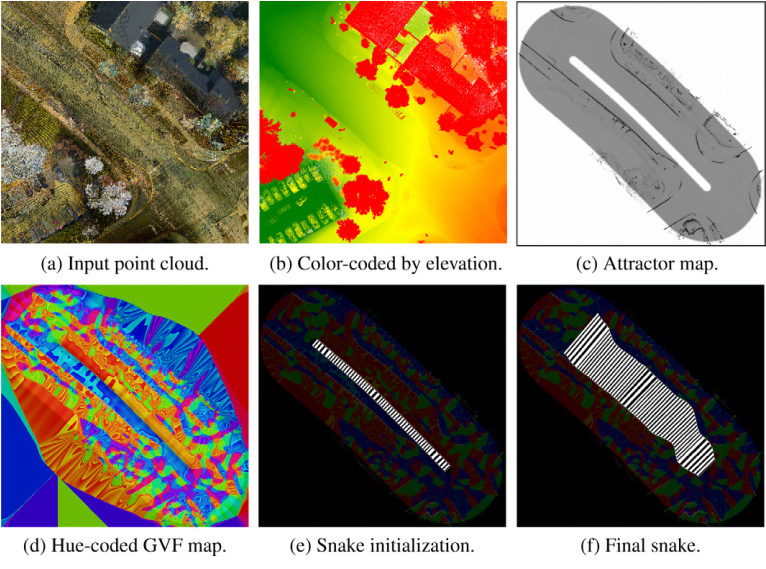
\includegraphics[width=0.85\linewidth]{final_report/figs/boyko_funkahuser_2011_01.png} 
    \caption{Illustration of the contour optimisation procedure used in \cite{boyko_funkhauser_2011}.}
    \label{fig:boykofunkhauser2011}
\end{figure}

The point cloud is then partitioned on disk, based on fitting support planes along the 3D-converted lines and fetching points that are close to them, solving performance-related issues of working with too many Lidar points at once, and further minimising the effects of 2.5D violations related to overlapping features. They then construct scalar maps for each resulting segment that penalises points away from road edges (both inwards and outwards). These maps, called attractor maps, are composited from rasters penalising locations that are outside the range in which edges are expected to be found (relative to the centrelines), and rasters produced by a curb detection metric related to the normal vectors of the point cloud points. Lastly, they apply an active contour optimisation technique (specifically, ribbon snakes) that yields the road edges in 3D, and then labels points between the two edges as road points. An illustration is shown in Figure \ref{fig:boykofunkhauser2011}, taken from their paper. In the attractor map, darker colours represent stronger attraction, resulting in the active contour converging to them in the optimisation procedure. The GVF map is a vector map that contributes to favourable active contour convergence and is not described any further here (please refer to the original paper). The initial contour is based on the road centreline (from external vector data).

The results of \cite{gopfert_etal_2011} demonstrate that active contour optimisation can be used to estimate road outlines without the need for the involved pre-processing steps of \cite{boyko_funkhauser_2011}. They convert the input point cloud directly into a DTM, and then into attractor maps. They use the same general type of active contour optimisation, and generate output centrelines and road edges with comparable quality to that of the outputs of \cite{boyko_funkhauser_2011}. It is worth mentioning that the type of active contour optimisation used by these two papers also optimises the road centrelines in conjunction with the road edges, which is particularly important in places where the 2D georeferencing of the original centrelines is poor.

\subsubsection{Relevant work with Dutch data}

The work \cite{oudeElberink_vosselman_2006} is relevant not only because of the methods it applies, but also the specific datasets. They enrich the best-known Dutch open data national topographical vector dataset (the present-day equivalent of which is BGT) with elevations, and as their source of elevations, they use AHN data (the first edition of AHN, the third edition of which I used in my own research).

\begin{wrapfigure}{O}{0.5\textwidth}
    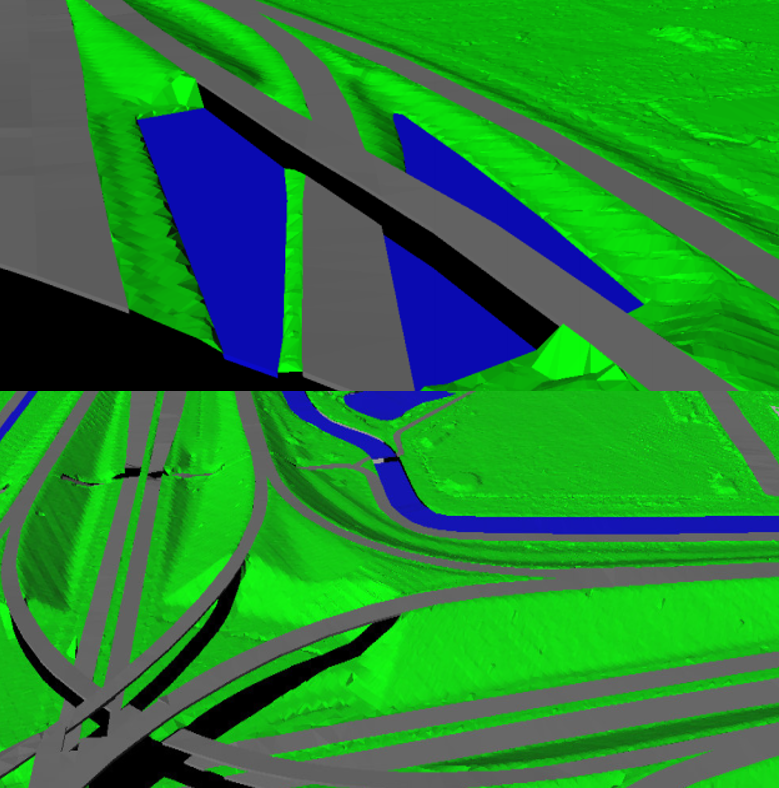
\includegraphics[width=\linewidth]{final_report/figs/oudeElberink_vosselman_2006_03.png} 
    \caption{Examples of 3D-converted multi-level road vector geometry from \cite{oudeElberink_vosselman_2006}.}
    \label{fig:conversionartefacts}
\end{wrapfigure}

They do not exclusively consider roads; all polygonal vector objects are extruded to 3D. Like in \cite{hatger_brenner_2003}, a region growing approach is proposed as the foundation of the elevation extraction workflow. They use the Hough transform to find seed points whose neighbourhood suggests a planar structure, fit planes and then grow them by checking the point-to-plane distance of new points, labelling points with the identifier of the plane they belong to. The vector data is then overlain on these regions and for each polygon, the plane is selected which is represented by the greatest number of labelled points in its interior. These points are re-fitted a plane, and each such plane is used to extrude the corresponding overlain vector geometry simply by projecting the polygon onto its surface. To improve upon the results of this simple extrusion, they suggest the application of algorithmic topological corrections. Furthermore, to model the interior of the extruded polygons in more detail, they recommend the construction of a Constrained Delaunay Triangulation (CDT) for each, first by inserting its edges as constraints, and then by inserting the Lidar points that its surface is based on. The CDT can be refined procedurally to ensure smoothness. The main limitations of their methods are that the extracted elevations (from the region growing approach) are not reliably accurate, and that it cannot handle overlapping objects, such as roads in motorway interchanges. 3D visualisations of the results of this approach and typical artefacts are shown in \ref{fig:conversionartefacts}. The specific artefacts shown in the figure demonstrate that in multi-level road layouts, only the topmost road is fully converted to 3D.

Their method was later extended in \cite{oudeElberink_vosselman_2009} to work well in complex multi-level road settings by using point cloud segmentation in a manner resembling what I already described in the context of \cite{boyko_funkhauser_2011}, which we may regard in general as decomposing the 3D problem into 2.5D sub-problems, also a main aim of my own research. In his doctoral thesis \cite{oudeElberink_2010} he combined this method with the overall procedure in \cite{oudeElberink_vosselman_2006} to form one integral whole. Furthermore he extended it with a road extraction quality and accuracy assessment procedure, which was later perfected and also published separately in \cite{oudeElberink_vosselman_2012}.

Their quality and accuracy assessment methodology is comprised of two separate procedures and the comparison of their results: a theoretical (error propagation-based) evaluation, and an empirical one against reference data. Their error propagation-based evaluation takes into account metrics such as GPS and INS noise in the Lidar survey (suggesting that they had access to low-level information about the dataset), plane fit quality and observed Lidar noise. It also considers interpolation/extrapolation uncertainty, relevant in places where not enough relevant Lidar points could be located and thus such gap-filling measures were used. They found that these theoretical errors were generally below 20 cm, with noticeable increases only occurring where Lidar coverage was extremely sparse or non-existent, leading to the necessity of using interpolation or extrapolation. 

Interestingly, their reference data was DTB for the empirical evaluation of accuracy, which is also the support dataset I used in my research (see Section \ref{sub:dtb}). In general, their comparison with DTB showed good agreement with their road surface extraction results, except for the same places where the theoretical approach also suggested large errors, and in particular in places where this was also combined with intense vertical road curvature locally, which DTB managed to capture, but not their results. In places with good Laser coverage, the agreement was much better, often near-perfect. Although not explicitly mentioned, it appears that they still used the earliest version of AHN (not AHN2) in this research, which may explain how it is possible that they encountered low point densities even in well-exposed road segments. AHN2 and AHN3 no longer have this problem, as mentioned in \ref{sub:ahn} and in many other subsequent parts of this report.

\subsubsection{On using a support dataset in addition to Lidar data}

In Section \ref{sec:input} in this chapter, I discuss that this research is also concerned with  another source of elevations, which I often refer to as the "support dataset" in this report because AHN3 is given priority to in the analysis, wherever it exists. It is a 3D line dataset, not an ALS or MLS point cloud. The one area \textit{not} explicitly covered in any of the papers I examined is the use of such external 3D vector data as a further constraint when extracting road elevations and/or geometries from point clouds.

In relevant work, occlusion is generally accepted to represent gaps in coverage, and elevations are simply interpolated or extrapolated inside them if possible - or if not, they are not considered any further. In the case of my research, NDW is interested in producing a 3D conversion of NWB with the highest possible \textit{completeness}. Exploring how information from the two datasets can be combined is also interesting academically, thus my work will examine how DTB can be used to patch in gaps in AHN3 coverage. While doing so, I will be building solely on my own ideas, as I could not find work that is directly relevant to this topic.

\section{Lidar accuracy and sampling density}
\label{sec:lidaraccuracy}

Relevant aspects of Lidar-related accuracy assessment can be divided into two main sub-topics: interpreting the reported global and/or local accuracy and areal sampling density of the Lidar surveys themselves, and assessing the accuracy of digital terrain models (DTMs) that one may derive from Lidar point clouds, and the elevations that can be interpolated from them. Although some of the relevant work I studied overlaps with both of these areas, I separated the discussion below into two sections based on them. As Lidar sensing accuracy and sampling density underlies that of the derived models, I discuss it first below.

\subsection{Accuracy description of Lidar sensing}
\label{sub:lidaraccuracy_sensing}

\subsubsection{Global and local influences on accuracy}

\begin{wrapfigure}{O}{0.46\textwidth}
    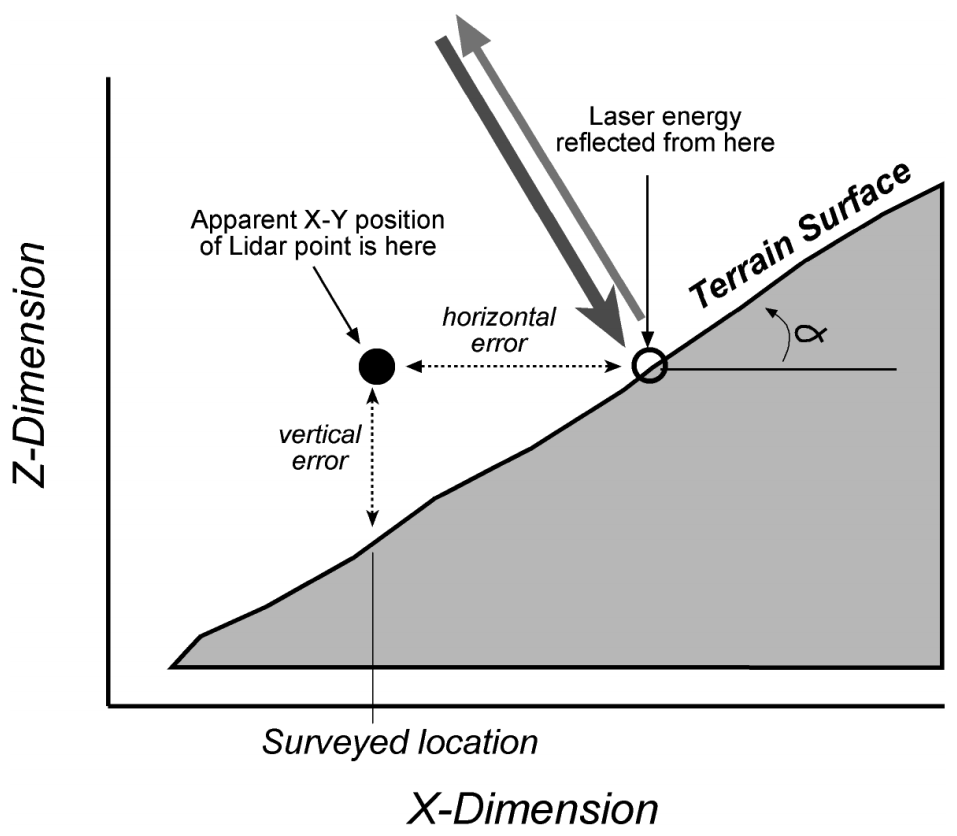
\includegraphics[width=0.95\linewidth]{final_report/figs/hodgson_breshanan_2004_01.png} 
    \caption{Illustration of the effects of terrain slope on vertical accuracy from \cite{hodgson_breshanan_2004}.}
    \label{fig:elevationaccuracy}
\end{wrapfigure}

Many papers describe that the accuracy of Lidar-derived DTMs depends primarily on the accuracy of the sensing method itself. The notable paper \cite{hodgson_breshanan_2004} describes the most fundamental sensing errors of Lidar measurements to be introduced by Global Navigation Satellite System (GNSS, such as GPS) errors, Inertial Navigation Unit (INS) errors, Inertial Measurement Unit (IMU) errors, errors introduced by the waveform analysis algorithm and lastly, a general error factor that depends on the flying height. Combined, these are the primary factors that contribute to the \textit{measurement} accuracy of the sensing system.

It is shown by various papers including \cite{hodgson_breshanan_2004, su_bork_2006, kraus_etal_2006, raber_etal_2007, peng_shih_2006, chow_hodgson_2009, aguilar_etal_2005, aguilar_etal_2010, guo_etal_2010} that there are local factors influencing \textit{vertical} Lidar accuracy that are independent of the sensing equipment, and thus vary from survey to survey. In production datasets, whether they are considered at all or not, they are almost never \textit{reported} locally, i.e. on the level of individual measurements. This is mainly because they are difficult to estimate without a complex analysis of the measured data and potentially, that of external data. Unless the global errors reported in the survey's specifications were derived empirically (e.g. by using ground control points), the effects of local factors specific to the survey may not be reflected in them at all, and they can be considered purely theoretical sensing-related values.

\subsubsection{What influences measurement accuracy locally?}

First and foremost, local accuracy depends on the inclination of the surveyed terrain at the point where the Lidar reflection occurred, as shown in Figure \ref{fig:elevationaccuracy}. Any uncertainty in the lateral position of the point of reflection will be scaled by the tangent of the slope angle, denoted by $\alpha$. The vertical error thus increases linearly as a function of increasing slope (commonly derived from a 2D slope map). Therefore, if the accuracy of a Lidar survey was derived empirically, it will indicate higher errors than the sensing equipment's specifications would suggest, in survey areas with considerable relief.

Elevation accuracy also depends on the vegetation encountered. In all cases, the presence of vegetation decreases it, with the significance of the error depending strongly on the type of vegetation. Mature trees and evergreens tend to influence accuracy to a lesser extent, whereas bushes, shrubs and undergrowth in general tend to have a decidedly larger impact. \cite{peng_shih_2006} quantified this as a function of \textit{vegetation angle}, a qualitative metric that describes how "open" certain types of vegetation are to Lidar. They found that there is a linear correlation between elevation errors and vegetation angle, as well as canopy volume. The one exception I found is \cite{raber_etal_2007} which reported specifically that in very strongly vegetated areas, no correlation could be found between vegetation classes and accuracy (or even point density and accuracy). Still, the majority of relevant research indicates that Lidar accuracy reflects the extent and type of vegetation coverage in addition to its dependence on the relief of the surveyed terrain.

Both the official quantification of measurement accuracy and research tackling these topics often uses empirical methods. They generally consist of surveying ground control points accurately and either directly comparing these with nearby Lidar points, or first constructing a spatially continuous DEM and comparing the DEM-interpolated elevations with the surveyed reference elevations, with the latter approach being more relevant to the next section. The global value is usually specified as the measurement error (in metres or centimetres) at one or two standard deviations, with separate values given for horizontal and vertical errors. The two errors differ in terms of the equipment influencing them, and also because the local factors I outlined above affect elevation accuracy only (as a \textit{function of} horizontal accuracy in the case of local terrain slope). They are generally reported as one or two standard deviations, corresponding to 68\% or 95\% confidence, in metres or centimetres.

\subsubsection{Sampling density as a survey property}

Sampling density describes how many reflections the sensor records per unit area. This is the third descriptor that is commonly found in the documentation of Lidar datasets, and like vertical and horizontal accuracy, it is generally represented by a single global value. This, too, fluctuates locally, and in this case anything between zero and the maximum nominal value of the survey's sampling density is possible. The maximum possible value depends on the sensing equipment and the number of times any given area is scanned (the number of passes). Sampling density does not directly affect the accuracy of individual Lidar measurements, which is one of the reasons why it is reported separately - its effects are more relevant to the next section.

Sampling density is mostly reported as the mean number of points per square metres found in the dataset, occasionally as a range if one or two standard deviations are taken into account. It can be derived from the data directly, i.e. it needs no additional processing or surveying. Relevant studies report that sampling density varies mostly as a factor of terrain relief, vegetation cover, and vegetation angle, with increases in any of these factors resulting in decreases in local point density. For instance, sampling density falls off logarithmically with increasing terrain slope (\cite{peng_shih_2006}, \cite{chow_hodgson_2009}).

\subsection{Accuracy description of Lidar-derived DTMs}
\label{sub:lidaraccuracy_dem}

\subsubsection{Spatial interpolation in the context of DTMs}

In practice, the quality and accuracy of Lidar-derived DTMs is most commonly evaluated via sampling their surfaces to serve as the basis for comparisons. Sampling a DTM takes place via spatial interpolation. The DTM's relationship with the raw data can be established by interpolating at the horizontal locations of Lidar points, while that with the real-world terrain can be examined via surveying control points and interpolating at their 2D positions in the DTM. Intuitively, DTMs provide a link between ground control points and Lidar measurements, which in turn also provides a convenient interface for evaluating Lidar survey accuracy empirically (as I mentioned in the previous section), provided that interpolator's effects on accuracy are known.

Raster DTMs are themselves produced via spatial interpolation. One may convert a Lidar point cloud into a TIN-based DTM without interpolation (the TIN vertices will be Lidar points), but to create a raster DTM, one will need to use a suitable interpolator, such as Inverse Distance Weighing (IDW). Alternatively, a TIN-based DTM can be constructed as an intermediate model and the raster can be derived from it via applying a TIN-based spatial interpolator, such as the Laplace interpolator. These observations entail that a comparison between the Lidar points and their TIN-interpolated counterparts would yield no residuals, i.e. TIN models do not lose information relative to the \textit{ground reflections} found in the Lidar data.

\subsubsection{Evaluating interpolation accuracy}

Spatial interpolators do not leave accuracy unchanged, which cannot be neglected when performing the above benchmarks. For us in this research, the effect interpolators have on accuracy is particularly interesting because the final NWB elevations are produced via spatial interpolation in a Lidar-derived DTM. There exist various approaches to establishing the nature of the relationship between input and output accuracy, such as deriving exact error propagation formulae from the mathematical descriptions of interpolators, as well as the more popular empirical approaches based on \textit{testing} accuracy post-interpolation via split-sample, cross-validation or jack-knife methods. Theoretically, input accuracy (survey accuracy) and any necessary metrics of local influences can then simply be plugged into the formula to obtain the local accuracy post-interpolation.

\subsubsection{Propagating local factors through interpolation}

However, we know from the previous section that the survey accuracy is \textit{itself} influenced by local factors. Since only global accuracy values generally exist for Lidar surveys, the theoretical or empirical error propagation formula may need to be extended with additional terms approximating the influence of these additional factors, depending on how accurately one wishes to approximate output accuracy. The exact nature of this part of the relationship depends on the fundamental principles I outlined in the previous section, and it too, can be modelled both theoretically and empirically. Theoretical approaches are more common for simple relationships (such as that with local slope, as shown in Figure \ref{fig:elevationaccuracy}), while empirical ones are almost always employed in more complex ones (such as the relationship with vegetation). In the context of digital terrain modelling, there is an additional factor we need to consider: ground filtering accuracy. While we wish to model the terrain surface only, the raw Lidar data includes non-terrain reflections that need to be removed before constructing the DTM. This accuracy is also generally estimated, rather than derived theoretically. It is also possible to try to derive the combined effects of all these factors at once, e.g. via Monte Carlo simulations.

For instance, the research \cite{aguilar_etal_2010} applies a hybrid empirical-theoretical method, in part propagating errors mathematically through the IDW interpolator to obtain part of the relationship, and for the other part relying on Monte Carlo simulations. They model accuracy to be a factor of the error-propagated value computed from global Lidar accuracy, as well as sampling density, terrain slope and ground filtering accuracy. The research \cite{kraus_etal_2006} also applies mostly theoretical methods to analyse errors propagating through the moving Maximum Likelihood Estimator (MLE). Post-application statistical evaluation was performed by for instance in \cite{peng_shih_2006} (jack-knife, using surveyed reference points), and \cite{guo_etal_2010} (ten-fold cross-validation). Notably, \cite{smith_etal_2005} used all three approaches (split-sample, cross-validation, and jack-knife) for a wide range of interpolators in an urban setting.

Like \cite{aguilar_etal_2010}, many of the other papers also examined the influence of gridded DTM resolution on accuracy, i.e. the effects of Lidar sampling density in conjunction with the raster cell size. \cite{chow_hodgson_2009} examined via regression techniques (on IDW interpolation) how it is correlated with point density and found that the effect of increasing the cell size has a more severe negative effect on accuracy than that of gradually decreasing sampling density, and that a certain degree of correlation between them is observable. \cite{guo_etal_2010} argues that for most interpolators, the overall trend is mainly linear between accuracy and grid resolution, up to the scale of the Lidar point density, from where no further increase is observable. They also found that differences in accuracy between interpolators were most prominent at the finest resolutions they examined. \cite{bater_coops_2009} found that the local influence on accuracy of slope and point density are mostly invariant relative to DTM resolution, i.e. no correlation is observable. In the case of TINs constructed from Lidar points directly, cell size and point density are in a more direct relationship, i.e. only by ignoring Lidar points can one increase the cell (triangle) sizes.

\subsubsection{Which interpolator is the best in terms of accuracy?}

In terms of the accuracy and quality ranking of interpolators, there is a clear consensus that no such ranking exists that is independent of the size and type of the study area, and the purpose of the interpolation. For instance, the accuracy of piecewise spline-based, quintic-type, kriging and ANUDEM methods were found lacking in the context of their insensitivity to small, sudden changes (such as natural faults in the terrain and anthropogenic modifications thereof) while they were proven to work well for large-scale terrain, as described by \cite{bater_coops_2009} and \cite{guo_etal_2010} for instance. All reviewed papers agreed that the accuracy of all interpolators decreases the most in areas of \textit{high topographical relief} (also called surface ruggedness and surface heterogeneity) and \textit{reduced point density}, with spline-based, IDW methods generally producing the worst results in such areas - especially for large-scale terrain.

The relative importance of interpolation-introduced errors is reportedly \textit{low} relative to instrument-related errors and surface-related local sources of error, according to research such as \cite{hodgson_breshanan_2004} and \cite{aguilar_etal_2010}. The former, which used TIN-linear interpolation, goes as far as to state that the decrease in accuracy after the application of an interpolator is insignificant, or that interpolation may even increase the overall accuracy. This is supported by the error propagation formulae derived by \cite{fan_etal_2014} for the same interpolator, which shows that in areas with negligible relief, the input error may decrease by as much as 50\%. TIN-based interpolation methods were recommended specifically by \cite{bater_coops_2009} for complex geometries and found it in their research to be the most conservative in terms of RMSE analysis. Furthermore, \cite{peng_shih_2006} also used TIN-based interpolation in their research, in which they found local influences on elevation accuracy highly predictable. Unlike most papers, \cite{aguilar_etal_2010} considers the accuracy of ground filtering explicitly, and states that its success is a precondition of accurate terrain interpolation wherever the terrain is occluded or shaded partially.

\subsubsection{Oversampling the terrain}

The point is made in several of these papers that because of the commonly seen logarithmic correlation between point spacing and accuracy, increasing the target point density of a survey is only justified up to a certain point. This depends strongly on the study area because point density itself is correlated with the vegetation cover and the terrain relief. It is argued by several authors, most prominently by \cite{guo_etal_2010}, that in vegetation-free areas of low relief, most ALS surveys oversample the terrain by as much as 30 to 50 percent, leading to increased processing times, reduced algorithmic stability, and no improvement in accuracy. \cite{bater_coops_2009} comes to the same conclusion, and the logarithmic trend generally observed between point density and elevation accuracy further supports this. Conversely, in rugged, vegetation-covered terrain additional cross-flight surveys can increase accuracy significantly by improving ground point density, as \cite{peng_shih_2006} noted.

The matter of oversampling the terrain is particularly important when using TIN models, because they use the Lidar points directly and may become too complex to process and visualise when they become too detailed. Considering the above correlations between point density and most other influences on accuracy, we may then assert that for flat, well-exposed surfaces the sampling density may not need to be high. This is particularly important in the context of this research, because roads represent such surfaces in most places.

\section{Input assessment}
\label{sec:input}

In terms of comparing our results with the commercial ones, we were particularly interested in revealing how the effectiveness of the two sets of methods differ. To make it straightforward to isolate differences related strictly to how well the methods perform, we decided to use the same set of datasets as input, as RHDHV. This means that in addition to using NWB, we made use of the same two elevation sources as they did.

In addition to helping with isolating purely processing-related differences between the results, these datasets have the additional benefit of being open data. This fits well with the mentality represented by those concerned with this research, as well as the faculty in general. For the same reason, the implementation created as part of this project is also made available in the same manner, i.e. it is open-source. Alternatives, such as Kadaster's orthoimagery-based point cloud were considered, but eventually excluded from further consideration, due to not being open data, and offering inferior overall accuracy compared with AHN3 and DTB.

\begin{itemize}
\item Nationaal Wegenbestand (NWB, National Road Database)
\item Actueel Hoogtebestand Nederland 3 (AHN3, Current Dutch Elevation)
\item Digitaal Topografisch Bestand (DTB, Digital Topographic Database)
\end{itemize}

In the sections below, I will present the result of assessing the general properties and quality of each of the three datasets listed above. As this project does not specifically concern the formal quantification of the accuracy of these datasets, it will rely on the global, nominal values provided in the specifications of the datasets. Regardless of this, I still present qualitative results on this topic based examining the degree of agreement between them and attempting to explain the differences based, both below and in Chapter \ref{chap:r}.

\subsection{Nationaal Wegenbestand – NWB}
\label{sub:nwb}

\begin{figure}
    \centering
    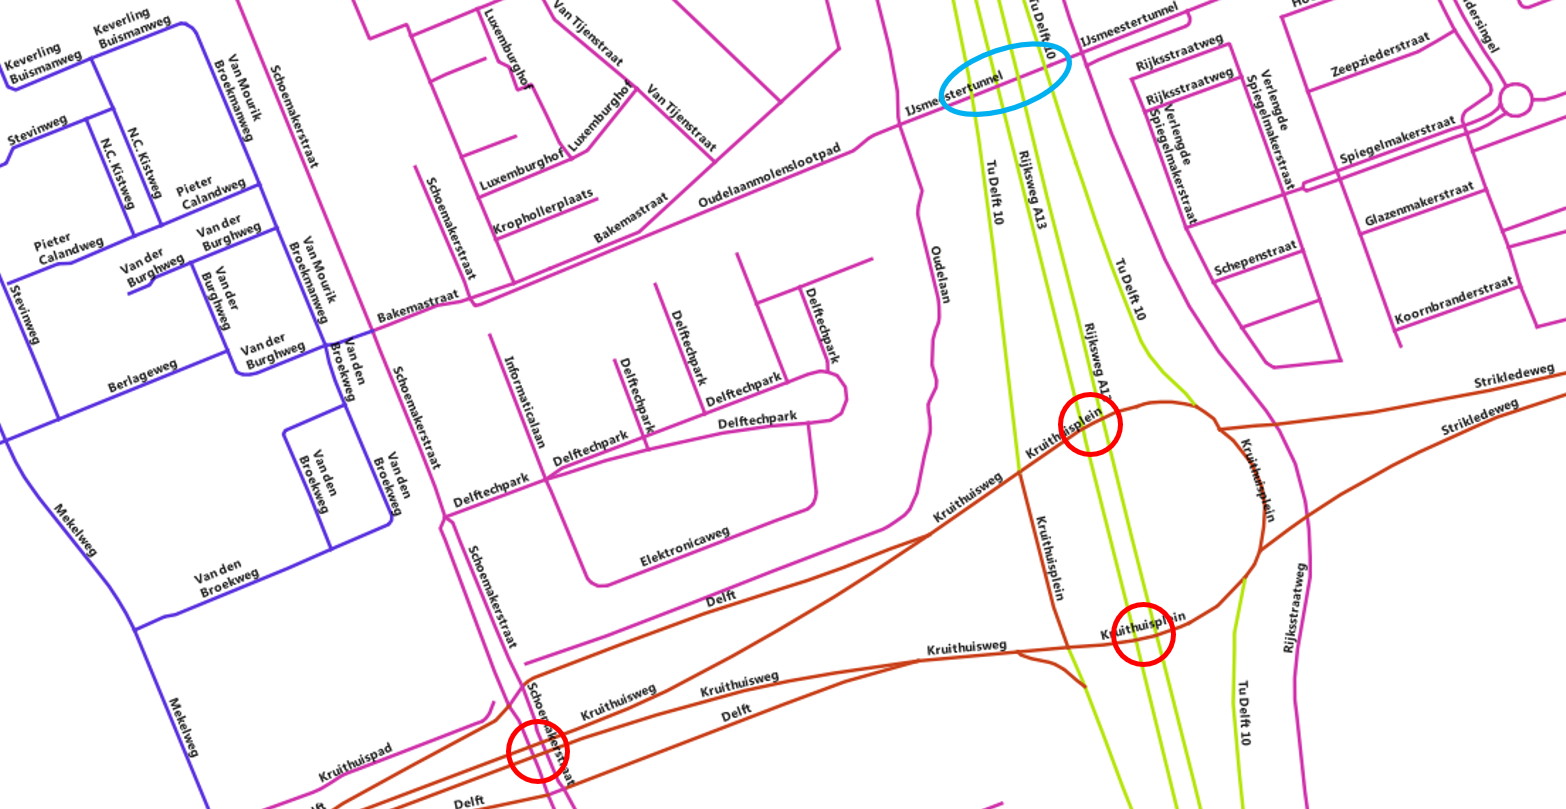
\includegraphics[width=\linewidth]{final_report/figs/nwb_sample_02.png} 
    \caption{An example render of NWB, colour-coded to indicate the owner.}
    \label{fig:nwb}
\end{figure}

NWB (or more specifically, NWB-Wegen, the NWB roads product) is a vector dataset comprised of a semantically enriched set of 2D \textit{MultiLineString} objects released in the \textit{ESRI Shapefile} format. They LineStrings are interconnected in such a way that NWB can be regarded topologically as a graph representation of the Dutch road network. Although NWB contains all named and numbered roads in The Netherlands, we are only interested in roads that are semantically marked as state-owned or province-owned (category R for Rijk and P for Provincie), because the new noise regulation only concerns these types. The NWB product is managed by NDW, but it is owned by RWS (NDW being a division of RWS).

NWB and the road types it contains are illustrated in Figure \ref{fig:nwb}. Yellow is used for R-roads (state-managed roads), red denotes P-roads (province-managed roads) and magenta means G-roads (municipality-managed roads). W-roads (RWS-managed roads) are not shown in this figure. Blue roads (T-roads) are roads which do not fall into the above 4 categories, in this case they are managed by the TU Delft. This render also contains examples of challenging 3D relationships. Where the P-road Kruithuisweg/Kruithuisplein crosses the G-road Schoemakerstraat and the R-road A13, no intersection occurs in 2D because the roads cross over one another in 3D. These locations are indicated in the figure by red circles. Furthermore, where the bike path IJsmeestertunnel (a G-road in NWB) crosses the A13, a series of 3 short tunnels are located in reality. This is indicated in the figure by a blue oval. Although not all these road types are relevant to this project, the 3D relationships represented by these examples still are.

In addition to representing the topology of the road network, the NWB lines are georeferenced with mediocre accuracy to also represent its approximate spatial layout. The quality description includes only a single figure, which is 5 m accuracy at 95\% confidence, i.e. two standard deviations from the mean. It is not described in any detail, how the accuracy is evaluated for each road, for instance whether it is based on the accuracy of the vertex locations of the road, an arbitrary sampling along their length, and how exactly these are aggregated into the error figure. Furthermore, we do not know whether the reference for the accuracy assessment was empirical (surveyed control points) or whether it is purely theoretical and is based on the sources and the methods involved in creating and updating the dataset.

Adding to the uncertainty is the fact that both the topological and the geographical information content of NWB is assembled from a wide range of providers ranging from large national providers such as RWS and Kadaster, to local providers such as specific road authorities and civil engineering agencies. No clear indication is given in the documentation about the sources used for the compilation of specific NWB road types or the estimation of their accuracies, but it is mentioned that they are not the same (\cite{nwb_docs}).

In interpreting the 5 m accuracy, it is important to note that the NWB lines represent road centrelines, but not of the whole paved surface. The centrelines in NWB approximate the centre of the traffic-occupied parts the roads, excluding hard shoulders and other paved surfaces connected to the road. It is also important, that NWB often does not contain vertices for more than 200 m based on my inspection (where roads are relatively straight), and even in sharp bends for up to 20-30 m at a time. Especially in bends, this circumstance, combined with the official error figure, means that NWB often leaves the traffic occupied road surfaces, and sometimes even the paved areas. I confirmed this problem by comparing NWB with DTB, AHN3.

One such comparison is shown in Figure \ref{fig:ahnnwb}. AHN3's ground points are coloured blue in this figure, and NWB centrelines are shown in white. As they have no elevation, they appear below AHN3 points and are consequently masked out partially by them. I shifted them to match AHN3's mean elevation locally, to make them better comparable. Comparisons such as these reveal that NWB gets close to the edges of the paved surfaces quite often, and sometimes even leaves their surface. In sharp bends, this is made worse by the angularity introduced by the coarse lengthwise discretisation of NWB, for instance in the location pointed out by the green arrow. In later stages of the project, I made further comparisons with the BGT and with orthoimagery (Luchtfoto 2020 from Kadaster), discussed in Section \ref{sub:completeness} and with an example shown in \ref{fig:bgtcomparison}. These comparisons further confirmed the issues.

Although the above nominal accuracy and its description are certainly not good enough for compliance with the new noise regulations, the 3D conversion of NWB is not concerned with improving it – in fact, it is a requirement of the project not to displace NWB horizontally. Hence, we may say that the intended outcome of the 3D conversion is to devise a method that can produce accurate elevations for NWB \textit{assuming} that its accuracy complies with the requirements set by the new noise regulations - 20 centimetres at 95\% confidence. To achieve this compliance in practice, lateral refinement is being carried out in a separate project by matching NWB roads with their counterparts in other, more accurate datasets. Specifically, DTB is being used for this purpose, as well as another open data dataset called Basisregistratie Grootschalige Topografie (BGT). As these datasets are already theoretically compliant with the accuracy requirements, correcting NWB geometries based on them will foreseeably solve the lateral accuracy problems of NWB. However, at the time of writing of this report, the BGT-based correction has only been released for municipality-owned roads (category G for Gemeente - not relevant to us), while the DTB-based corrections for motorways are still being finalised. Consequently both the commercial and the scientific 3D-NWB project still rely on NWB data that lacks this correction (\cite{nwb_gecorrigeerd}).

Regardless of improving NWB’s lateral accuracy not being within the scope of this project, it is important to be aware of it, because of its implications when overlaying NWB with AHN3 and DTB in the processing part of this research. The problems caused by it and the necessary workarounds are discussed in-depth in the relevant sections of the next chapters.

The NWB product is updated every month with particular attention to always including new roads, removing outdated (demolished or permanently closed) roads and updating refurbished roads as necessary. This frequency means that NWB is always up-to-date with changes to the road network, at least to the extent where navigation (in e.g. Google Maps, which uses NDW) can take place without any disruptions. However, this does not mean that NWB has a temporal resolution of one month; for that to be true, all roads would need to be re-measured every month. The monthly releases merely mean that effort is concentrated into releasing known changes to the road network frequently. Since no physical phenomena exists that would move the roads laterally (without human intervention) by a significant distance, this does not cause issues in practice.

\begin{figure}
    \centering
    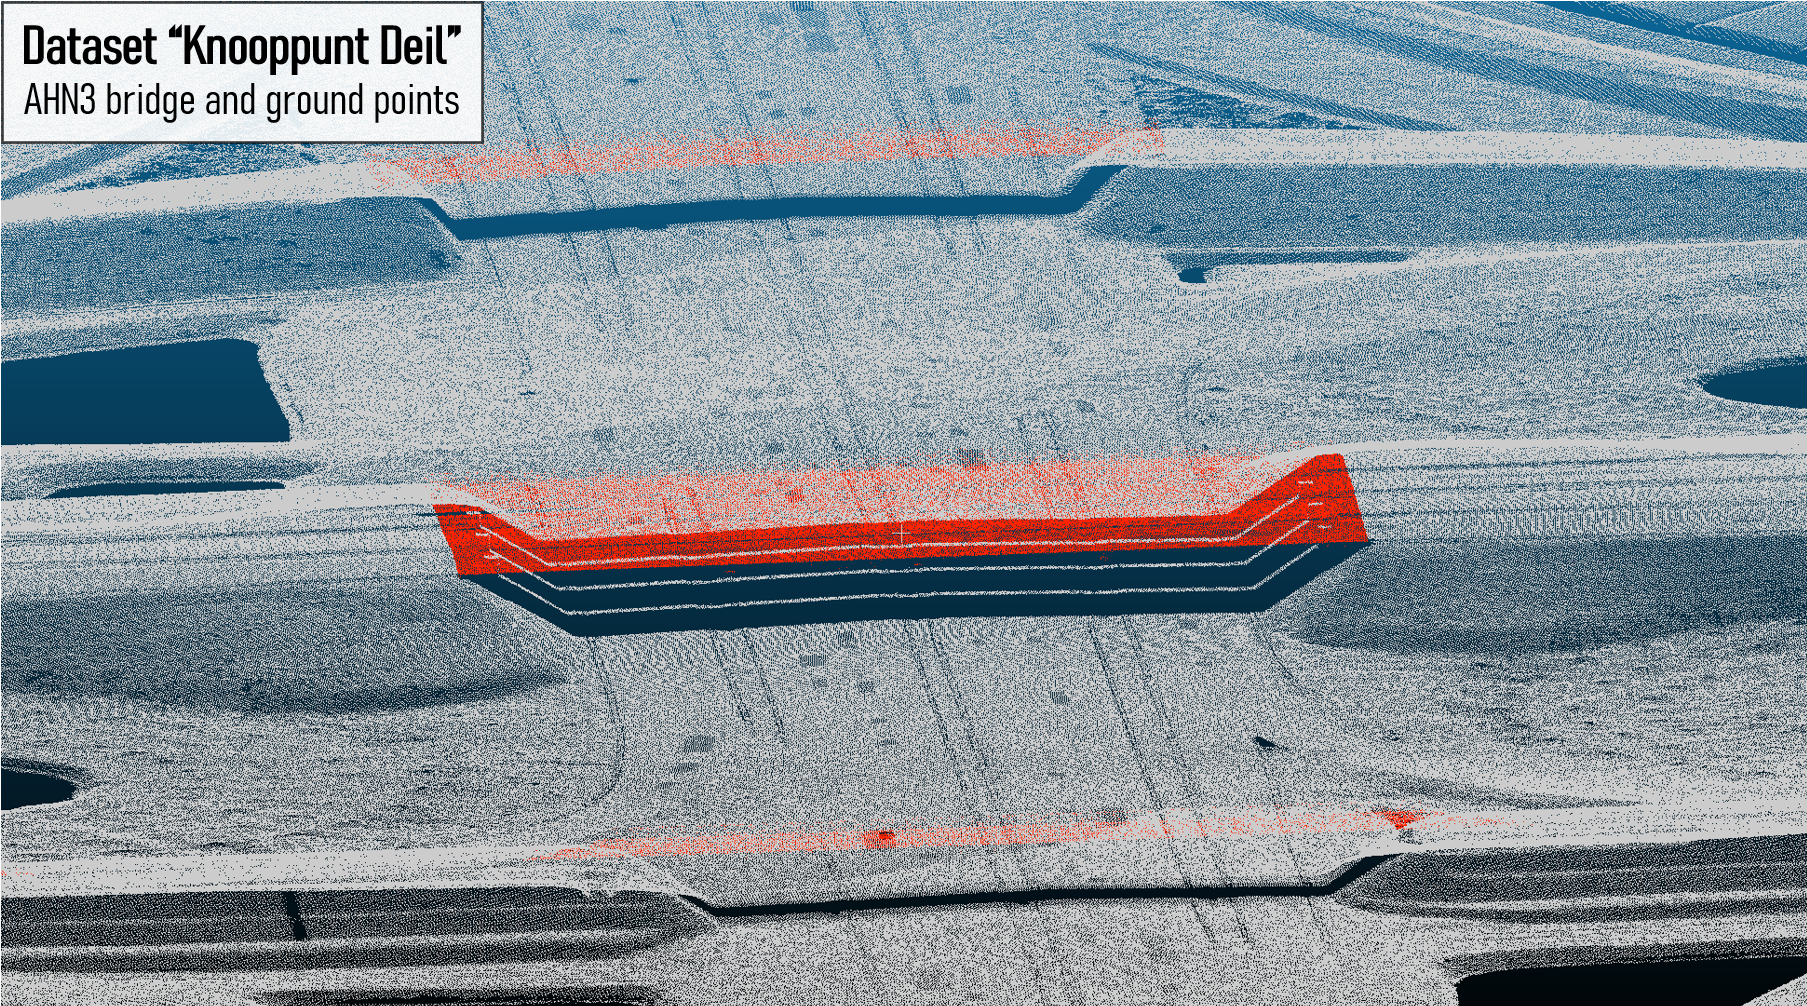
\includegraphics[width=\linewidth]{final_report/figs/ahn_sample_01.png} 
    \caption{Example render of AHN3 at Knoppunt Deil, SW of Geldermalsen, showing ground points and bridges.}
    \label{fig:ahnbridges}
\end{figure}

\subsection{Actueel Hoogtebestand Nederland – AHN}
\label{sub:ahn}

AHN are airborne Lidar (ALS) survey datasets available as open geospatial data in The Netherlands. The surveys are commissioned every few years with AHN (the first version) to AHN3 already complete (1996 to 2019), and the first AHN4 tiles nearing release. At this stage of the project, we are interested only in AHN3, as it is te most recent iteration of this product. The AHN product is owned and managed by RWS.

The dataset has a combined systematic and stochastic elevation error of 15 centimetres at two standard deviations (i.e. 95 \% confidence), and 6 to 10 points per square metre point density on average, corresponding to a 0.32 to 0.41 metre posting distance. The lateral error is 18 centimetres at two standard deviations (\cite{ahn_kwaliteit}). Comparing these to the descriptors of Lidar datasets used in the research examined as part of our literature review (see the Relevant work section), we may assert that AHN3 can be considered accurate, and to have excellent point density. It is especially accurate and dense relative to the older Lidar datasets that are mentioned in these papers, including the first iteration of AHN.

The AHN3 point cloud has been classified semi-automatically with similarly excellent accuracy and is released with the classification included. This means that for most purposes, the point cloud needs not be ground filtered by users, and that extracting certain features is made far easier. Of the various classes available, we are interested in class 2 the most, which corresponds to ground points, and class 26 which contains, among other things, bridge structures and the roads that are found on them.

Ground points are primarily interesting to us because they contain the points reflected from land-based roads. This includes roads that were constructed directly on the terrain, as well as roads constructed on altered terrain, such as elevated ground or open trenches. It also contains the points that represent the terrain in the vicinity of the roads. Elevated roads and bridges are not considered ground points and are generally represented by gaps in class 2, which can, in most cases, be filled by using data from class 26, as shown in Figure \ref{fig:ahnbridges}. The white colour corresponds to ground points (class 2), red corresponds to bridges (class 26). All other classes were removed. The shapes of motorway lanes and ramps, as well as bridges are clearly defined. Road constructed on elevated ground is reliably classified as ground, bridges are cleanly split off by the classification. Even under thin bridges, data becomes gradually sparser at the border and becomes extinct directly below the bridge. This render also makes it clear that wherever vehicles were encountered on ground-based roads, the sampling is worse locally. It does not \textit{generally} go entirely extinct however, as most locations have been scanned multiple times. Data gaps are only observed where slow or stationary vehicles wer encountered.

Class 26 also contains other types of objects, for instance large motorway signs arching over road surfaces, as well as the civil engineering structures of elevated roads and bridges (in addition to the road surfaces on them). Reflections from vehicles transgressing bridges are also present in this class. Figure \ref{fig:ahnsigns} shows a render from the same location as \ref{fig:ahnbridges}. The full-width motorway signs are clearly visible above the motorway lanes, coloured red because they originate from class 26. It also shows that the presence of water results in holes (the dark, linear features running parallel with the motorway in this render) in the ground-only point cloud. In this render, it is also visible that in my testing datasets, all points falling outside a 150-metre buffer zone around the NWB centrelines were removed (see more information on this in Section \ref{sub:testingdata})

\begin{figure}
    \centering
    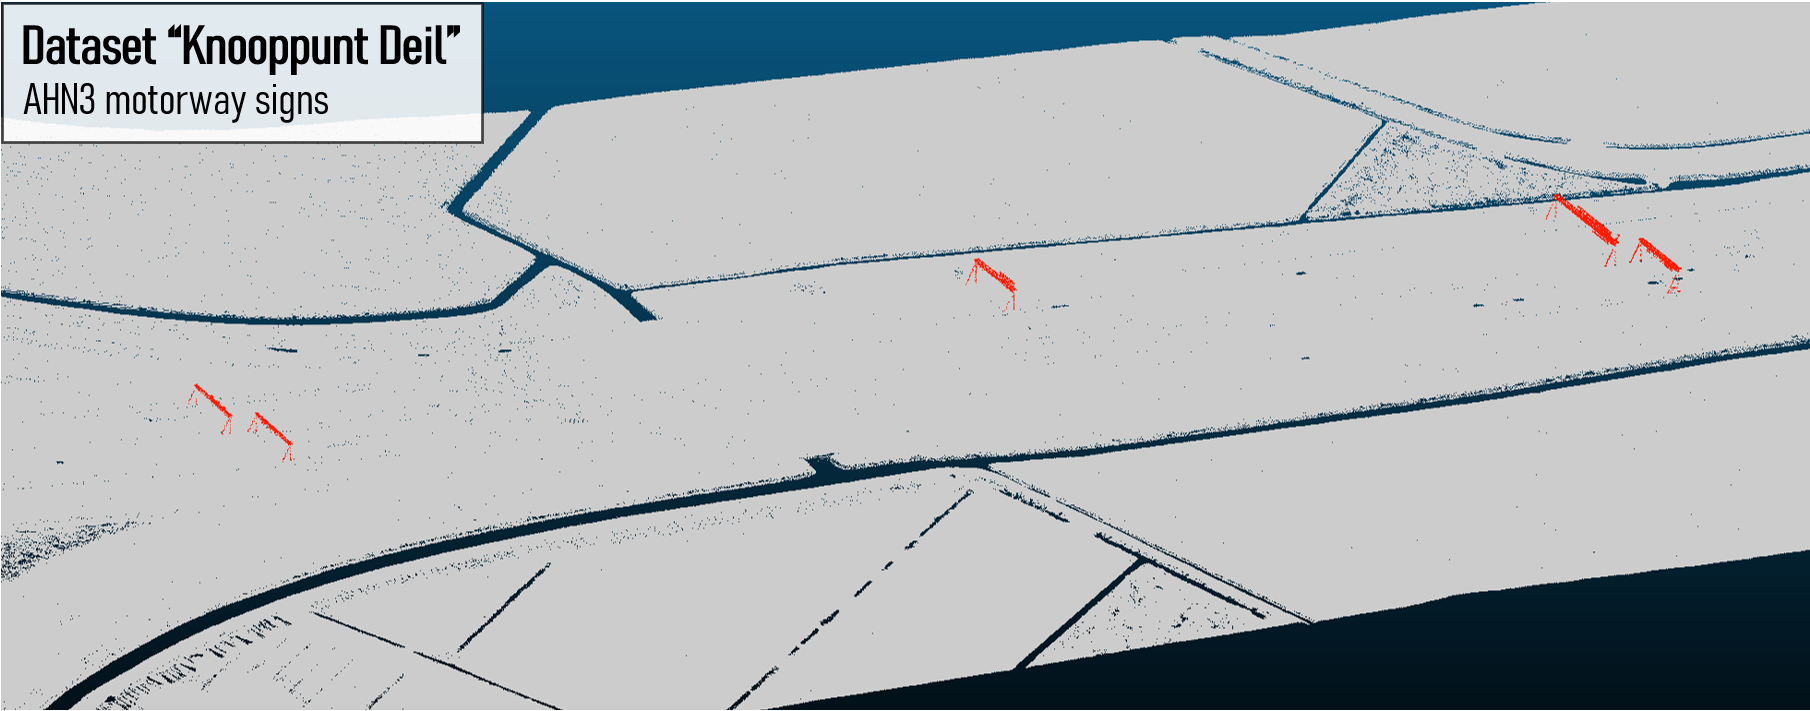
\includegraphics[width=\linewidth]{final_report/figs/ahn_sample_02.png} 
    \caption{Example render of AHN3 at Knoppunt Deil, SW of Geldermalsen, showing ground points and motorway signs.}
    \label{fig:ahnsigns}
\end{figure}

\begin{figure}
    \centering
    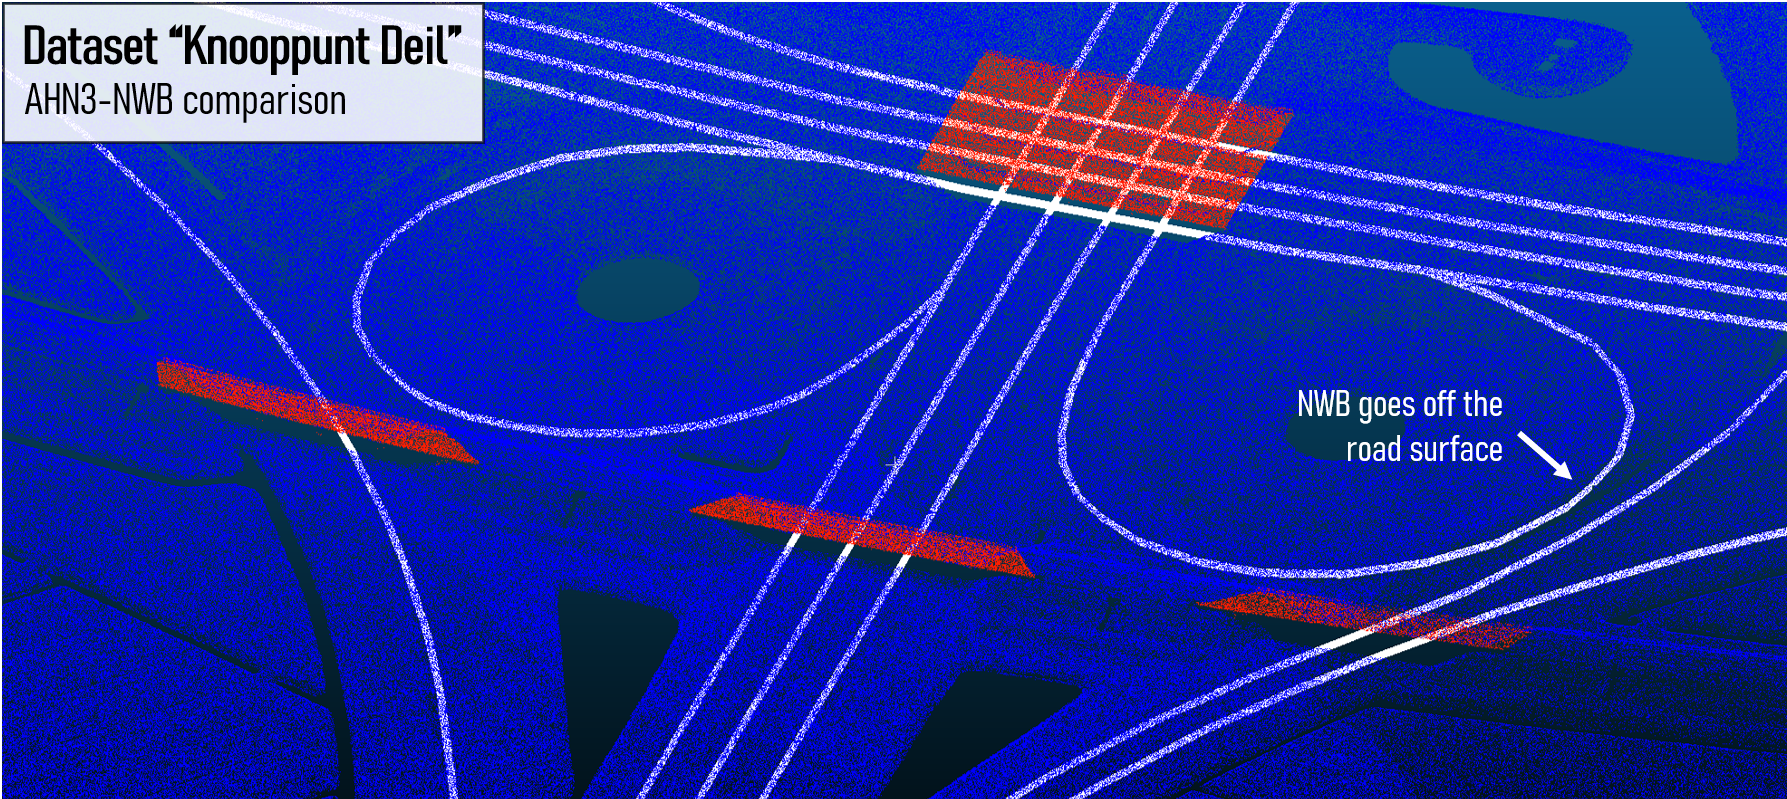
\includegraphics[width=\linewidth]{final_report/figs/ahn_sample_04_a.png} 
    \caption{Render comparing AHN3 with the relevant 2D NWB centrelines.}
    \label{fig:ahnnwb}
\end{figure}

AHN3 is released in the form of a point cloud, as well as DSM and DTM rasters. Both were produced using basic radial IDW interpolation with a fixed parametrisation. The DTM was generated by including only points from class 2 in the interpolation step. They are available at 0.5-metre and 5-metre resolutions, with the 0.5-metre resolution being relevant to this project in terms of the target accuracy. For context, this raster converts (on average) 1.5 to 2.5 points into a single raster cell based on AHN3's nominal sampling density. The commercial implementation uses these rasters, as explained in Section \ref{sub:commercialproduct}.

The Lidar tiles are released in the binary LAZ format (compressed LAS, or LASzip), and are generally several gigabytes in size. As each tile only covers an approximate area of 32 square kilometres and the LAZ compression ratio for this dataset is 0.1 on average, scaling considerations are relevant to this project if the implementation is to be capable of fully converting NWB to 3D using the raw point clouds rather than the rasters.

\begin{figure}[h!]
    \centering
    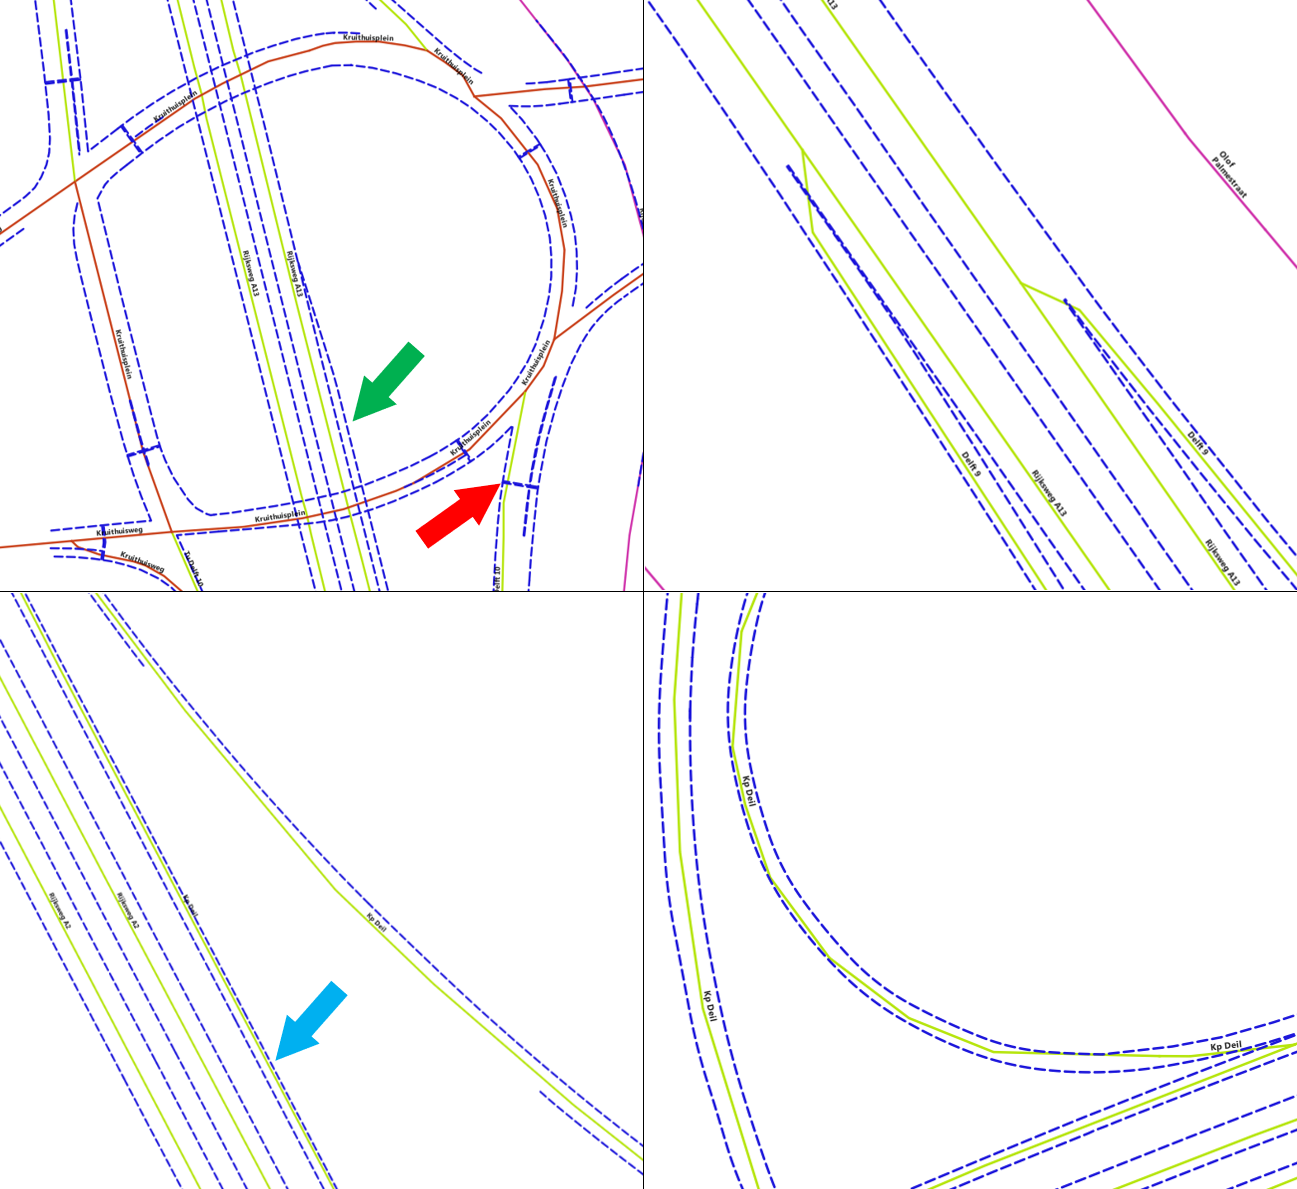
\includegraphics[width=0.95\linewidth]{final_report/figs/dtb_sample_07.png} 
    \caption{Renders of DTB \textit{verflijnen} overlain with NWB centrelines, illustrating "compatibility issues" and individual DTB issues.}
    \label{fig:dtbnwb}
\end{figure}

\subsection{Digitaal Topografisch Bestand – DTB}
\label{sub:dtb}

\begin{figure}[h!]
    \centering
    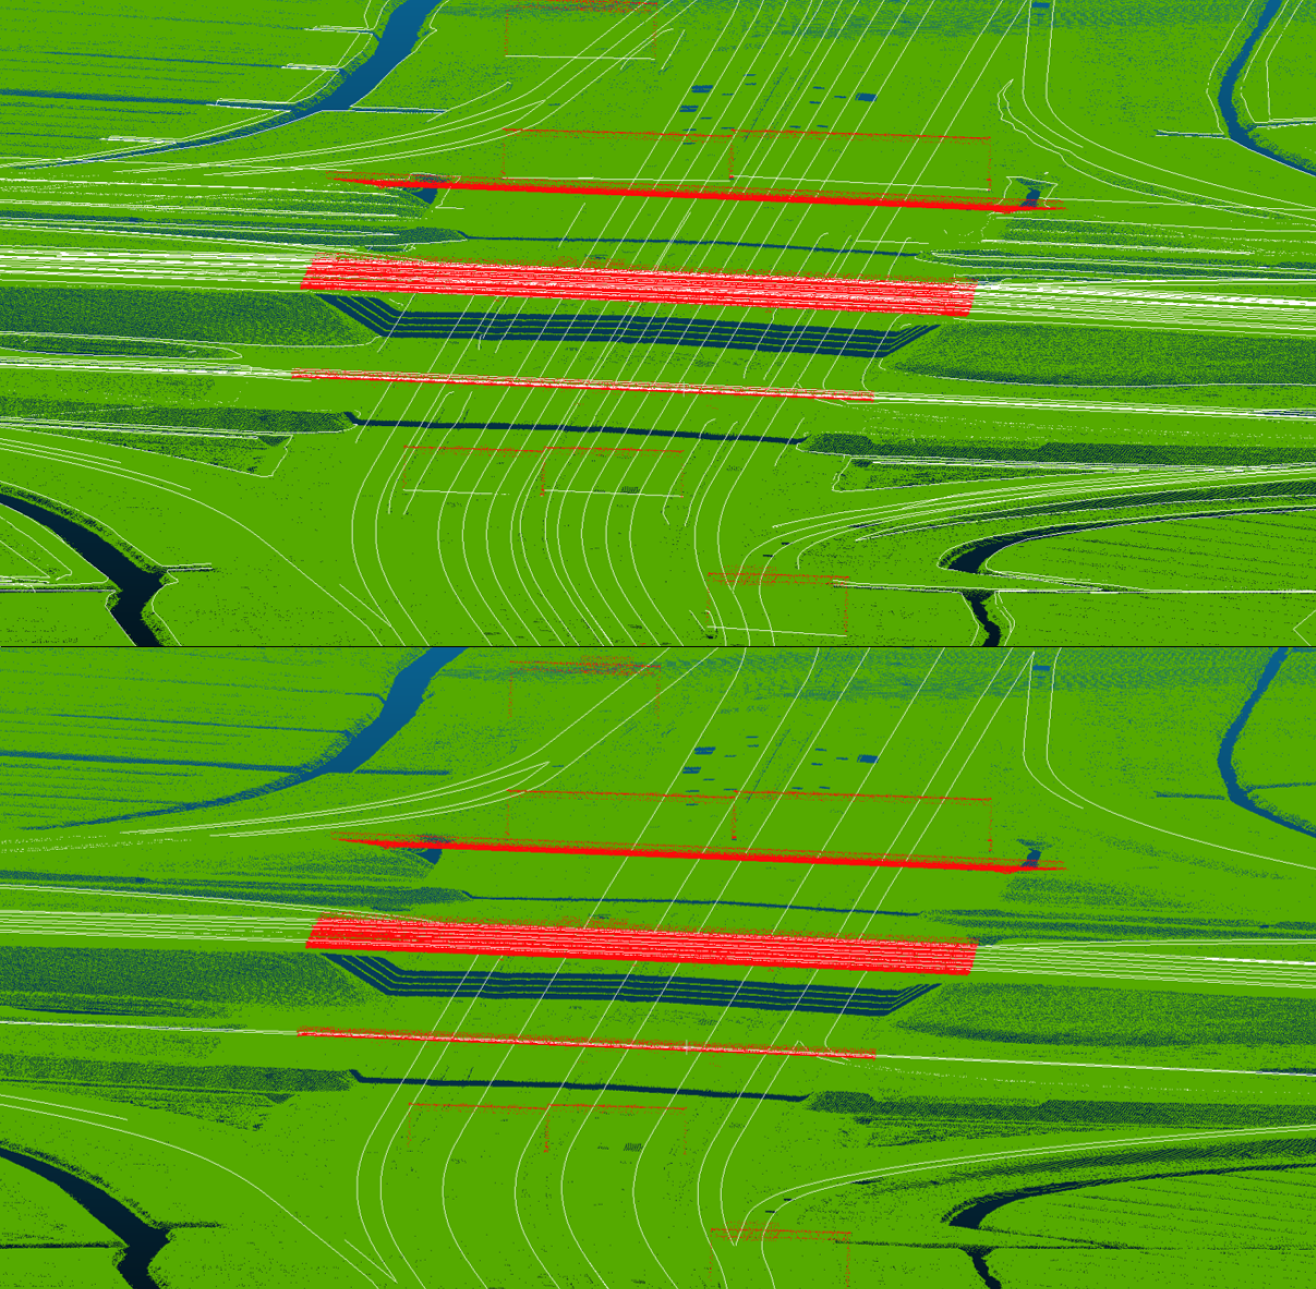
\includegraphics[width=0.95\linewidth]{final_report/figs/ahn_sample_10.png} 
    \caption{Renders of DTB line features overlain with AHN3 in 3D.}
    \label{fig:dtbahn}
\end{figure}

Like NWB, DTB (or more specifically, DTB-Droog, the DTB product relevant to roads) is a Dutch open data geospatial dataset in the \textit{ESRI Shapefile} format. For the purposes of this project, we only need only those DTB line features, which correspond to street surface markings, hence we can also regard this as a dataset comprised exclusively of \textit{MultiLineString} objects, making it identical to NWB in its data structure apart from being a 3D dataset. DTB is also managed by RWS and it is concerned only with state-owned roads and roads on state-leased land, which translate almost exclusively to NWB R-roads, that is, motorways. DTB is, hence, not a reliable source of information about provincial roads elevations (NWB P-roads), our other road type of interest.

There are various types of DTB road markings that are of interest to us, the main one being a category called \textit{verflijnen}. These DTB lines represent the painted lines marking the outermost edges of the area open to traffic. This is a lucky correspondence with NWB, as it too, contains the centrelines of the areas of roads that are open to traffic. The other two types I found to be reliably represent road surface elevations are the categories \textit{verfstippellijn} and \textit{blokmarkering}, which are lane separation lines and block marks respectively. The category \textit{lijnverlichting} also appeared to be interesting at first, as it corresponds to road surface lighting features (not street lighting). However, I found it to not be reliably located on road surfaces in practice, hence I excluded it from further consideration.

Figure \ref{fig:dtbnwb} shows a visual comparison with NWB, illustrating various types of significant issues that primarily stem from NWB's crude georeferencing. NWB symbology is identical to that which I used in \ref{fig:nwb}, and blue dashed lines are the DTB lines. Only \textit{verflijnen} are present in DTB in these locations. The image in the top left shows that in practice DTB contains many road markings, rather than just one on either side of NWB. The illustration in the top right shows that NWB motorway ramps often merge with the motorway lanes at unrealistic angles, causing NWB to intersect the DTB edge markings at these locations. The image in the bottom left illustrates that while in some places there are many DTB road edges, in other places they are incomplete or missing entirely. Furthermore, NWB centrelines may also get very close to DTB edges outside of sharp bends and motorway ramps, as indicated by the blue arrow. In the bottom right, the figure shows that NWB discretisation and inaccuracy leads to angular angular lines in sharp bends. NWB often gets close to, or even intersects DTB in such places.

Like NWB (but unlike AHN3), DTB’s production pipeline also concerns several organisations performing various types of sensing, which are then semi-automatically assembled into the complete DTB product. While many DTB features are photogrammetry-derived, road surface markings are mainly from accurate land-based manual surveys or extracted from car-mounted Lidar (MLS) data (\cite{oudeElberink_vosselman_2012}). The documentation of DTB consists of its formal specifications (\cite{dtb_docs}) and a handbook (\cite{dtb_handbook}). The former contains the accuracy-related details, reporting 10 cm vertical and 5 cm horizontal standard deviations, or 20 cm and 10 cm at 95\% confidence to make it comparable with the reported accuracy of NWB and AHN3.

Theoretically, DTB is not only accurate, it also has a good temporal resolution. It is updated multiple times a year, specifically to always be up-to-date in terms of newly constructed roads and refurbished roads - just like NWB. This update frequency is comparable to that of NWB, which is part of the reason why it forms part of the commercial solution. The other part of the reason is, that it theoretically always contains data for occluded roads, even in tunnels. This means that the combined information content of DTB and AHN3 theoretically amount to having complete coverage of the Dutch road network. Because of the ease with which elevations can be extracted from DTB to be used in the 3D conversion of NWB (especially considering the crudeness of NWB's georeferencing) prompted NDW to consider DTB as its \textit{primary} dataset, wherever it is available.

In practice, I found evidence to support that the above decision is fundamentally flawed, already during the input assessment stage of my project. There are places where DTB lives up to the above \textit{theoretical} standards, but this is not the case in most of the areas I examined. Even in terms of motorways, DTB is often incomplete to the extent that it lacks coverage over tens of kilometers. Even where it exists, its coverage may be patchy, especially in sharp bends. An example is shown in Figure \ref{fig:dtbnwb}. Commonly it only contains a single line rather than the theoretical minimum of three (two edge markings and one separation line). The separation line is the one I observed to be missing the most frequently.

Furthermore, already by considering the update methodology of the dataset, one may remark that some of the elevation measurements in it must be very outdated. Indeed, most of them are almost as old as the roads themselves, meaning that they were taken more than 20 years ago. This is where it comes into play that the update methodology of NWB and DTB does not really represent a high temporal resolution. In the absence of a physical phenomenon causing significant lateral ground motion, this does not cause problems with NWB, but there \textit{is} one that may move roads up or down: subsidence. Although the surface load due the weight of the road and passing vehicles may play a role, subsidence is primarily caused by natural, geological processes. In some parts of The Nethelands, groundwater and natural gas extraction may also play a role. Although this work does not specifically study the correlation between subsidence and problems with DTB, there is little else with which the 0.5 to 1 m differences between AHN3 and DTB could be explained. The AHN3 measurements are at least 15 years more recent than the oldest ones in DTB, which is where the biggest differences can be observed in elevation, as one would expect from subsidence.

Interestingly, the opposite can also be observed, although less commonly, and in a highly localised manner. In some places, DTB is above the road surface measurements of AHN3 by a significant margin, often by more than 0.5 m. While subsidence cannot be used to explain these disagreements, there is evidence to support that the elevations in AHN3 are indeed correct and the ground has shifted upwards noticeably. The latest subsidence survey of The Netherlands reported positive changes in addition to the decreasing elevations that are associated with subsidence. I primarily observed DTB to be below AHN3 where this map indicates negative elevation changes, and above in regions where no changes or slightly positive changes were observed in the subsidence study, verifying my hypothesis.

Figure \ref{fig:dtbahn} shows renders of DTB overlain on AHN3 with all DTB features shown (above), and with only \textit{verflijnen} shown (below). Ground points are shown in green. The top render illustrates that other features, such as roadside slopes, canals, ditches, safety rails are represented in DTB. Full-width motorway signs are also occasionally represented (either by lines on the road, or on the structure itself). The bottom render shows that locally, the edge markings are in good agreement with AHN3 visually, and are only occasionally incomplete. This location has the best vertical correspondence with AHN3, and also the best completeness, of all the areas I examined. For illustrations of the \textit{disagreements} between DTB and AHN3, please refer to Figure \ref{fig:lidarsegmentation1} and the associated discussion in Chapter \ref{chap:r}.

\section{Methods of existing implementations}
\label{sec:methodsexisting}

\subsection{NDW prototype}
\label{sub:ndwprototype}

NDW themselves produced a prototype implementation, which can achieve a 3D enrichment of NWB with only a few gaps in the produced elevation profiles. Although their workflow does not have a formal documentation, I have been given a verbal description of it, as well as the output. Based on my understanding of these, their primary technique involved snapping close-by AHN3 Lidar points to the line geometries of NWB. Notable problems with the implementation included non-road points being snapped to centrelines, causing road centrelines to be given overestimated elevations, in turn resulting in abrupt spikes in the elevation profiles.

Furthermore, no close-by points could be found for underground roads (i.e. tunnels), and strongly occluded parts of roads. For small gaps, this was resolved partially by writing an algorithm to interpolate linearly inside NWB, using the closest vertices where snapping was successful. For larger gaps, an attempt was made to resolve issues by including information from external sources semi-automatically. Neither issue could be fully resolved via these approaches, hence the results of this project were only used by NDW to gain a better understanding of the problem and the expected challanges. For the development of a reliable digital toolbox they subsequently commissioned a commercial implementation from RHDHV.

\subsection{RHDHV's commercial implementation}
\label{sub:commercialproduct}

RHDHV developed their implementation in parallel with the planning of the present scientific research. During this time, I attended NDW-RHDHV meetings, discussed the commercial system design and implementation details directly with RHDHV personnel, and was granted access to the codebase of the project. Understanding their implementation was crucial for the planning and realisation of my research, as it was among my goals to estimate the effectiveness of the commercial implementation's methods, as well as assess the quality estimate the accuracy of the their final results. In addition, creating my system design while learning about the known and suspected shortcomings of their methods allowed me specifically focus on areas where a different, less pragmatic approach could yield better results.

\subsubsection{Overview of system design}

First, where NWB vertices are too sparse, vertex densification takes place; i.e. additional vertices are created inside NWB line segments until all vertices are found less then a certain threshold distance from their neighbours. From then onwards, \textit{different} workflows are initiated for R-roads and P-roads.

For P-roads (where DTB data does not generally exist), the workflow is conceptually similar to the one in the prototype, with the notable difference of using AHN3 DTM rasters rather than the point cloud. Because AHN3 DTM rasters are badly affected by both large holes and small groups of missing pixels (due to the fixed-parameter IDW interpolation that was used to generate them), RHDHV could only make use of them by filling in the gaps of the raster using linear interpolation in a 3D TIN created from extruded raster pixel centres. They then simply interpolated elevations for NWB from the raster using bilinear interpolation. Intermediate results of this procedure are shown on the right in \ref{fig:rhdhv}. It shows a raster being overlain with NWB to yield elevation values. The raster still contains the holes that AHN3 rasters contain by default; these are filled in before interpolating elevations for NWB but are shown here for demonstration purposes. Two types of holes generally occur: small-scale ones due to objects such as street furniture, vehicles and vegetation, and large ones that are typically due to large-scale occlusion due to buildings or bridges (as in this case). The test build shown here used AHN2 rasters, but their production implementation uses AHN3.

\begin{figure}
    \centering
    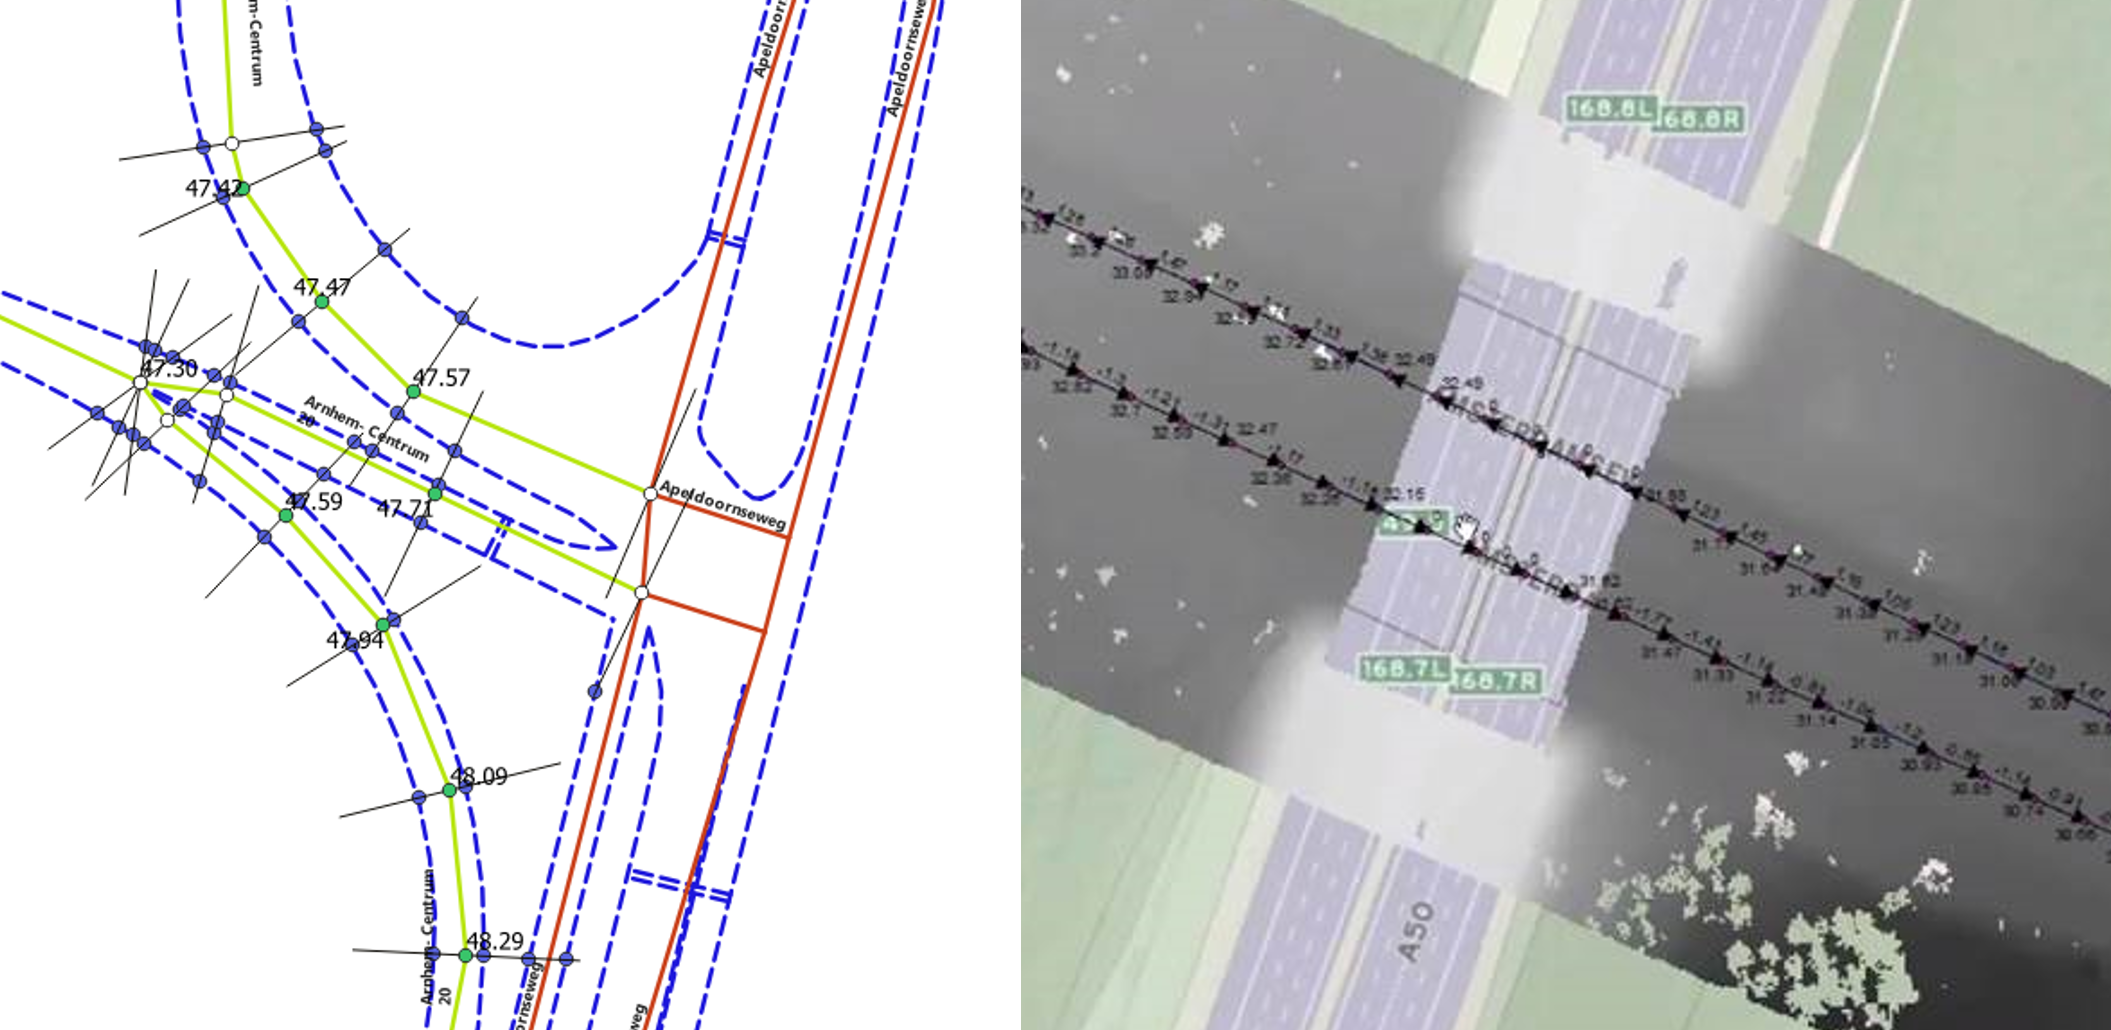
\includegraphics[width=\linewidth]{final_report/figs/rhdhv_combined.png}
    \caption{Illustrations of RHDHV's commercial implementation.}
    \label{fig:rhdhv}
\end{figure}

For R-roads, DTB is available, and the assumption is made that it is more accurate than AHN3 (or at least the stock DTM tiles generated from AHN3), to the extent where it should be the primary source of elevation data. Priority is thus always given to it in the procedure, with AHN-based interpolation used only as a fallback mechanism in case DTB-based height estimation fails for any reason (anomalous elevations computed, or missing DTB geometry).

The goal of the underlying algorithm is to find the closest, roughly parallel DTB line segments at any NWB vertex, and to deduce elevations from them. First, 2D cross-sections are constructed on NWB vertices, with each given the mean azimuth of the two NWB line segments that they are part of, and then rotated 90 degrees. For vertices created during densification, this simply means the rotated azimuth of their parent line segment. DTB lines are then intersected with the cross-sections and for each cross-section, the closest DTB line that satisfies a relative angle condition is picked on both sides of NWB. Elevation is then first linearly interpolated inside the two chosen DTB segments to yield values exactly at their intersections with the cross-section. Lastly, elevation is interpolated linearly along the cross-section itself to yield the final elevation at the location of the NWB vertex.

The angle condition I mentioned above is a threshold-based evaluation concerning the angle between intersected DTB line segments and the cross-sections, and is used to ensure that the chosen DTB segment is indeed roughly parallel to NWB locally. This helps ensure that the algorithm does not accidentally choose a DTB line segment that belongs to a different (underlying or overlying) road surface. The assumption is thus made that the DTB line segments representing surface features of a given road are roughly parallel with the relevant NWB centreline, and lie close to them. Implicitly, this also assumes that even if no other DTB road markings are present, NWB centrelines will still lie between two DTB road \textit{edge} markings, i.e. \textit{verflijnen}.

In practice, backup mechanisms needed to be implemented because these assumptions do not always hold. Primarily, this is because in sharp bends NWB may not be parallel with the relevant DTB lines locally, and because it is frequently not complete enough to be used for the above operations. To bridge these issues, wherever the algorithm only finds a suitable DTB intersection on \textit{one} side of NWB, it is only that side from which the elevation value is deduced. If no suitable intersection can be found whatsoever, the AHN3 raster-based interpolation is used instead (the same workflow that is always used for P-roads).

This procedure is illustrated on the left in \ref{fig:rhdhv}. The cross-sections that are constructed on NWB vertices are shown as black lines. Green circles denote those vertices where the cross section could be properly intersected with DTB lines (blue circles) and thus be given an elevation value. White circles denote where the procedure failed, and AHN raster-based interpolation was necessary. This render illustrates that in sharp bends the assumption that NWB and corresponding DTB lines are parallel does not necessarily hold, because of how coarse and inaccurate NWB's georeferencing is, especially relative to DTB which is very accurate horizontally. The render also illustrates that P-roads are not processed in this way, not even if they have DTB lines next to them (which frequently occurs in the vicinity of motorways).

\subsubsection{Potential limitations}

At the time of finalising this report, the results of the commercial implementation have already been made available to me and the comparison with my own results carried out. However, in this section I discuss the \textit{suspected} limitations of their methods, not the properties of their results. During the project planning, system design and implementation stages, the commercial results were not available to me yet and as a result, the bulk of my work - almost everything apart from Section \ref{sec:r_comparison} - is based on verbal descriptions of their methods and preliminary results.

First and foremost, I suspected that using AHN3 rasters in place of the point cloud would affect the quality of their conversion. Point cloud to raster conversion is, by definition, associated with inherent information loss (less raster cells than point cloud points), and further reduction in accuracy is introduced by the interpolation mechanism itself, that created the rasters. Radial IDW was used to generate AHN3 DTM tiles, which several of the reviewed papers found to be specifically unsuitable for interpolating large-scale areas in which zones of decreased point density or gaps exist – both of which characterise ground-filtered AHN data (e.g. \cite{guo_etal_2010}). In addition, the procedure performs another layer of interpolation to infill gaps, which may further deteriorate accuracy. Furthermore, RHDHV uses bilinear interpolation inside the raster to produce NWB elevations, which is suggested by \cite{shi_etal_2005}, to be less accurate than other common methods such as bicubic.

Furthermore, there is no mechanism built into the software to deal with occlusion in the case of P-roads, and also R-roads where DTB is unavailable. This means that wherever NWB elevations are interpolated in occluded road segments from AHN3 rasters, they will be incorrect. Just like in the NDW prototype, these values will show up as spikes in the elevation profiles, as well as longer bumps where wide features (e.g. bridges) are encountered. Since there is no outlier filtering or smoothing algorithm built into the software either, the severity of this issue is not mitigated in any way.

Based on the input assessment, it is also evident that prioritising DTB wherever it is available may itself be a questionable decision, in view of the fact that the output's accuracy needs to measure up to the noise regulation's expectations, at least theoretically. DTB is accurate horizontally, in fact it is theoretically more accurate than AHN3. However, even if its vertical accuracy was also satisfactory at the time of its acquisition, it no longer is, due to various degrees of vertical ground motion taking place in the country. As elevations in DTB are not updated where no civil engineering changes have taken place in the road network, its road surface markings are often far too outdated to be used with any certainty, especially considering that there is no reason to do so given that AHN3 contains equally accurate, but significantly more recent data.

Lastly, the commercial implementation lacks a formal accuracy assessment. Although this is common with comparable commercial products, in this case the output dataset needs to comply with formal accuracy \textit{requirements}. Without a quantitative or at least qualitative accuracy assessment of some form, there is not enough evidence to support the applicability of the commercial results to the noise modelling applications they are intended for.

Since the accuracy of AHN3 rasters is known and simple bilinear interpolation is used to obtain elevations from them, deriving output accuracy would not be difficult wherever their solution uses AHN3. This excludes interpolating in gap-filled pixels, which would need further considerations. In the case of DTB, the evaluation of accuracy may be equally simple, as the underlying computations all boil down to linear interpolation. However, wherever DTB data is old, any accuracy quantification would be meaningless because DTB itself does not comply with its own formal accuracy, due to vertical land motion.
%!TEX root = ../thesis.tex

\chapter{Methodology and methods}
\label{chap:mm}

This first section of this chapter presents a description of the methodology of the planned dissertation work. This description is limited to matters relating to planning the execution of the work, without going into specifics about the methods themselves. The second section of the chapter presents an overview of the methods themselves, including information about how these plans evolved since the P2. This section also includes detailed accounts of the thought processes leading to the most important design choices. The rest of the chapter is devoted to a detailed account of the methods that underlie each of the processing steps in the final "proof-of-concept" software implementation, with accompanying flowcharts to illustrate the system design represented by the methods. A short section at the end of the chapter describes the implementation's software architecture, with explanation about certain technical design choices regarding the implementation.

\section{Methodological framework}
\label{sec:methodology}

This section contains a written account of the key stages into which the execution of this research can be divided. Each subsection describes one such stage, discussing the specific tasks performed during each stage as well as what has changed relative to my original plans. The methodology is also visually illustrated on a flowchart in Figure \ref{fig:methodflow}.

\subsection{Preparation}
\label{sub:preparation}

This project concerns a client - NDW - with specific requirements and a pre-existing attempt at implementing a solution, in addition to aspects that are purely scientific. As a result, the first stage of the project involved \textit{consultation with the client} and with their commercial developers - RHDHV - in addition to the task of \textit{familiarising myself with the research topic and literature}. The results of these preparation tasks were \textit{discussed internally} with my supervisors and used to \textit{define the final list of formal research questions} on the basis of focusing primarily on academic topics while also fulfilling the requirements of the client. This combined knowledge was then used to \textit{produce the P1 submission}. This stage roughly coincided with Q1 of the academic year, and with the P1 period of the dissertation research.

I executed this stage of the project according to my initial plans, little has changed during its realisation.

\subsection{Preliminary analysis, proposal writing}
\label{sub:preliminaryanalysis}

The second stage of the project involved \textit{further consultation with the client and their developers} to determine to what extent the commercial and scientific branches of the 3D-NDW project could be linked, and to allow me to understand the exact methods used in the prototype and the commercial implementation (which was being actively developed during this period of time). In parallel with these tasks, I \textit{performed the necessary in-depth literature review} and preliminary analysis. The preliminary analysis was comprised  of a \textit{close examination of the input datasets and their documentations} (input assessment), and based on this and the research questions, the \textit{final selection of relevant concepts and methods}. I also selected a range of illustrative geographical regions during the preliminary analysis, and cropped the datasets to their extents to \textit{create testing input files} for later development and testing. Lastly, the results of this stage were distilled to \textit{produce the P2 document}. This stage roughly coincided with Q2 of the academic year, and with the P2 period of the dissertation research.

I executed this stage of the project according to my initial plans, but with a few small alterations. My initial plan was to put a slightly larger emphasis on performing preliminary analysis tasks, but the abundance of relevant literature and the complex task of creating a preliminary design for the methods (and the pipeline itself) limited the amount of time I could spend on it. I focused most of my effort at this stage in the research on the litrature review and the preliminary system design instead. This meant that during the next stage, I had a solid starting point in terms of background knowledge, and specific plans regarding what to start implementing.

\subsection{Analysis}
\label{sub:analysis}

The third stage of the research spanned the period between my P2 and P4 presentations. This stage concerned carrying out most of the analysis. The period was characterised first and foremost by the intense development effort focused on the \textit{implementation of individual algorithms and steps of the workflow}. My original plan was to isolate this set of tasks and perform it during the period between my P2 and P3 presentations, and to \textit{assemble the pipeline} from the individual modules after the P3. However, it proved to be more effective to develop the modules and incrementally extend the pipeline with them at the same time - an approach to which I switched after implementing the first few modules. This allowed me to resolve pipeline-level issues as part of the incremental refinement of methods, in addition to problems related to specific pipeline steps only.

Carrying out the \textit{accuracy-related analysis} was the last stage of the project that required active development on the program code. Testing the individual procedures and the pipeline was continuous during the implementation, with larger tests performed after reaching major milestones. Testing, and the assessment of performance and accuracy used the testing datasets I produced as part of the preliminary analysis. This was followed by a self-evaluation of the overall results of the research and a discussion of them with my supervisors, as well as a comparison of the commercial results and mines. The stage was concluded by \textit{writing the present draft thesis} ahead of my P4 presentation.

\subsection{Finalisation}
\label{sub:finalisation}

The last stage of the project will last a few weeks between the P4 presentation and the P5 presentation. Both \textit{the implementations and the present report itself will be improved and finalised} during this time. The final version of the source code and its documentation will be published in the project repository on GitHub. Furthermore, the outcome of the research and its findings relevant to improving the commercial implementation will be discussed with our client.

\begin{figure}
    \centering
    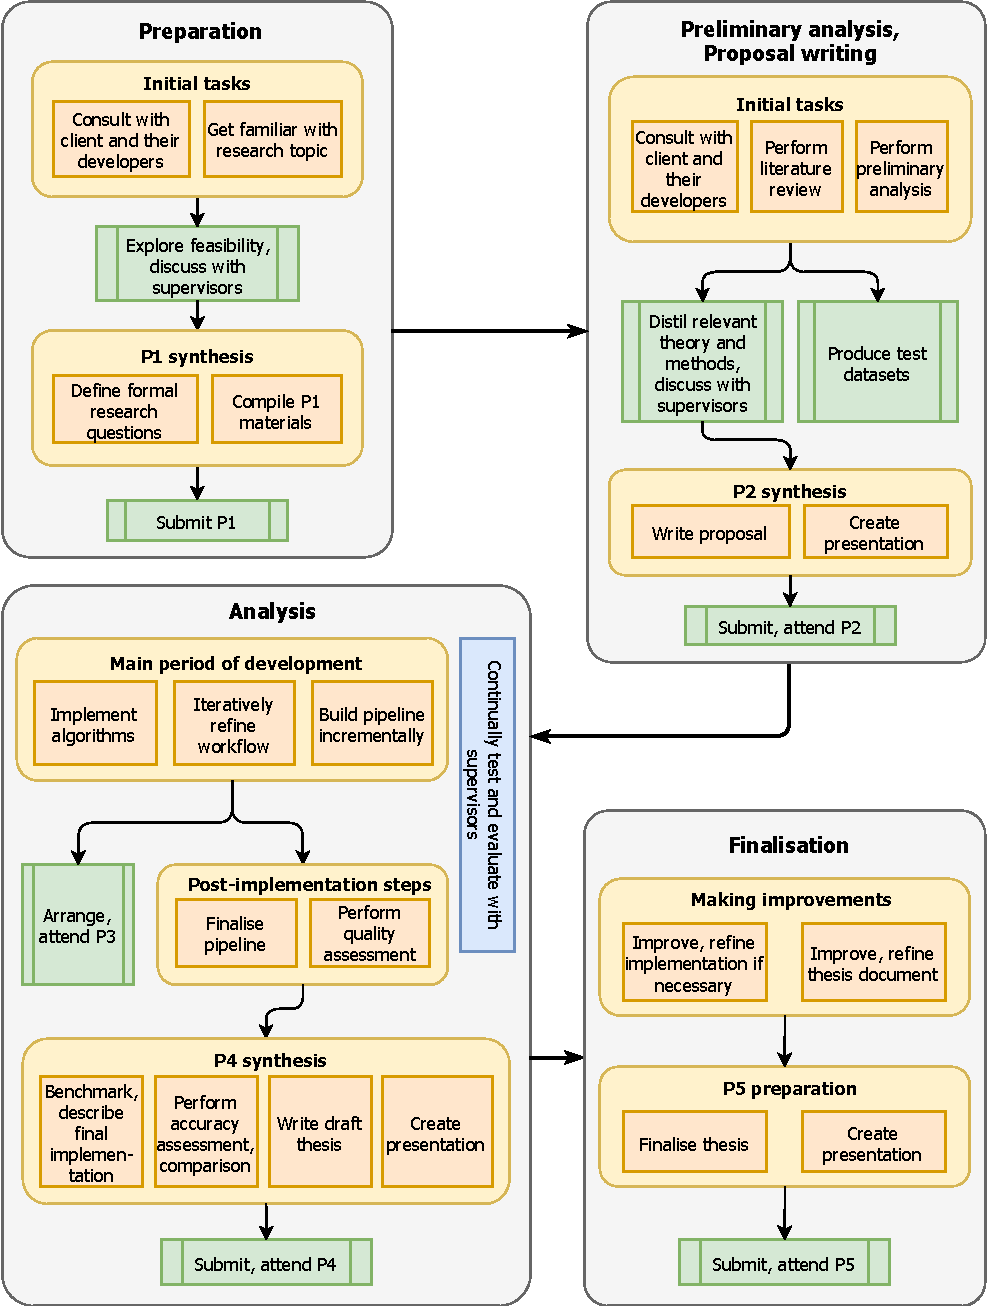
\includegraphics[width=0.9\linewidth]{final_report/figs/methodology.pdf}
    \caption{Flowchart-style illustration of the top-level methodology of my proposed dissertation research.}
    \label{fig:methodflow}
\end{figure}

\section{Overview of methods}
\label{sec:methodsoverview}

This section provides a structured overview of the steps of the processing pipeline. While the detailed descriptions in Section \ref{sec:methods} focus on explaining how exactly each step works, the purpose of the present section is to provide the rationale justifying their necessity and the reasons underlying certain major design choices, as well as to describe their role in the context of the system as a whole.

While the exact aims of the project materialised during the first two stages listed in Section \ref{sec:methodology} above, a brief description of the project existed before it. The project was originally conceived as a an academic continuation to the pre-existing attempt of NDW to implement a solution to the 3D conversion of NWB, re-using NDW's prototype implementation as the basis for a completed, academically sound version. During the aforementioned two stages, it became clear that NDW's pre-existing implementation is not robust and flexible enough to justify building the academic project on top of it. Hence, the entirety of the below pipeline was designed and implemented specifically for this academic project, no part of it represents code borrowed from the NWD prototype (or the RHDVH implementation).

\subsection{Proposed processing pipeline}
\label{sub:pipelineoverview}

The design of the pipeline is the result of a combined understanding of concepts described in related work, my own knowledge and experience relating to the geomatics discipline, as well as inspiration from the methods of the commercial implementation. The proposed workflow was built with a strong focus on finding answers to the research questions. Furthermore, it is also the result of a process of iterative refinement. In most cases, this only concerns the technical details of the algorithms implementing the pipeline steps, but in some cases I also made major changes to certain aspects of the general approach. Hence, in the structured overview below, I added a list item per pipeline step specifically to describe what changes, if any, were made to the given step.

As a brief summary of the general idea, the pipeline takes NWB, decomposes it into roads whose surface can be modelled by 2.5D methods, and applies a set of mostly geomatics operations to produce the 2.5D road surface models that the elevations are then derived from to produce 3D-NWB. Accuracy-related considerations are not yet described in this section, these are first discussed in Section \ref{sub:accuracyoverview} below. A visual illustration of the main pipeline steps is shown in Figure \ref{fig:workflowsteps}, showing only the titles of each workflow step in the order in which they are executed.

\begin{enumerate}
    \item \textbf{NBRS generation}
    \begin{enumerate}
        \item \textbf{Goal:} assemble optimal 2D profiles from the building blocks of NWB.
        \item \textbf{Approach:}
        \begin{enumerate}
            \item Assemble \textit{Non-Branching Road Segments}, henceforth referred to as \textit{NBRS} (in both plural and singular) from NWB geometry. To do so, look for series of NWB wegvakken (LineString objects) that represent the same road and join them into optimised 2D profiles - NBRS.
            \item Perform the assembly of NBRS in a way that maximises their length (optimal for lengthwise 2D operations such as polynomial fitting), minimising internal angles at the same time. Disallow self-intersection, so that each NBRS can be modelled in 2.5D.
        \end{enumerate}
        \item \textbf{Purpose:} this step is necessary, because in addition to working with small-scale (short wavelength) features in the road network, we wish to be able to inspect trends that take place over longer distances in the network. The building blocks of NWB (wegvakken) can sometimes be short, occasionally only a few metres long. Hence, assembling them into NBRS provides a better starting point for later steps.
        \item \textbf{Changes:} from the outset, I expected that simple methods based on progressing along 2D profiles, as well as modelling 2D profiles as a whole, would be useful for this project, and that a data structure serving this dual purpose would be necessary. Hence, NBRS have always been part of my plans and their exact specifications did not change much during development.
    \end{enumerate}
    \item \textbf{Preliminary elevation estimation}
    \begin{enumerate}
        \item \textbf{Goal:} create a rough, preliminary 3D version of NWB.
        \item \textbf{Approach:}
        \begin{enumerate}
            \item Based on the median elevation of nearby Lidar points, associate NBRS vertices with preliminary elevation approximates, thereby performing a crude 3D conversion of NWB.
            \item Perform polynomial fitting on the 2D profiles that NBRS represent. Identify vertices that are outliers with respect to the general shape of the NBRS and interpolate values for them linearly.
        \end{enumerate}
        \item \textbf{Purpose:} this step is necessitated by the next one, point cloud segmentation. While it is possible to perform it without first performing a rough 3D conversion, I found it to be much more effective when the approximate 3D locations of NBRS are already known by that point.
        \item \textbf{Changes:} this step represents and addition relative to the original plans. I started suspecting its benefits during the implementation stage, and subsequently added it to the pipeline design.
    \end{enumerate}
    \item \textbf{Point cloud segmentation}
    \begin{enumerate}
        \item \textbf{Goal:} using their preliminary elevations, find "patches" of Lidar points in the 3D vicinity of NBRS vertices. Progressing along the vertices of each NBRS in a linear manner, fit planes on their Lidar patches. Where an unexpected change in the plane fits is detected, rely on DTB to provide a reference and to help navigate through the ambiguous region.
        \item \textbf{Approach:}
        \begin{enumerate}
            \item Where DTB is also unavailable, accept the shifted (or missing) plane fits but perform a polynomial fit afterwards to identify planes that are unlikely to belong to the relevant road surface. Split the NBRS into parts in such places, excluding the undesired regions from further consideration until the last pipeline step. 
            \item Based on the plane fits, decide which points in the patches are relevant to the road surface represented by a given NBRS, and create subclouds by merging them (one for each NBRS part). Include DTB points that were used in places where AHN3 data was missing.
        \end{enumerate}
        \item \textbf{Purpose:} like NBRS generation, this step also has a dual purpose. Firstly, it associates each NBRS with a set of candidate Lidar and DTB points that are likely to be relevant to them, thereby reducing the amount of Lidar points that will need to be processed later on. Secondly, it also excludes the majority of points which are close to a given road, but which were reflected from occluding geometry instead of its surface.
        \item \textbf{Changes:} originally, I only wished to detect where plane fits become inconsistent to exclude small-scale occlusion at this point. However, I eventually realised that by tracking changes in certain metrics, I could do so even in relatively long occluded regions. I then incorporated DTB as a backup dataset to increase the reliability of this method, which made the solution work even where significant changes in elevation take place inside the occluded regions (such as in tunnels). I added the splitting of NBRS into parts as a last tweak, after implementing the rest of the pipeline. This improved the results of later steps by removing areas without AHN3 \textit{and} DTB coverage from the NBRS.
    \end{enumerate}
    \item \textbf{Preliminary edge approximation}
    \begin{enumerate}
        \item \textbf{Goal:} create line geometries on both sides of NBRS approximating the edges of the road surfaces.
        \item \textbf{Approach:}
        \begin{enumerate}
            \item construct cross-sections on NBRS vertices and convert them to 2D elevation profiles by sampling AHN3 along their length. Perform linear regression on each, and select the outermost stable inlier points on both sides of the NBRS. The two points are taken to represent the road edge locally.
            \item Assemble approximate road edges from the discrete edge points generated by the previous step, enforcing constraints regarding the expected shape of the road edges. Relax the constraints after a certain number of successive failures, to allow the algorithm to adapt to real-life changes in the road geometry.
        \end{enumerate}
        \item \textbf{Purpose:} the sole purpose of this step was going to be to provide edge estimates for active contour optimisation. After I made the decision to make active contour optimisation optional in the pipeline (due to its ineffectiveness), preliminary edges also became optionally needed for later steps, in place of the optimised contours.
        \item \textbf{Changes:} Due to the optional use of preliminary edges in TIN construction (in case optimisation is skipped), I needed to improve their quality significantly. This entailed the implementation of significant refinements to the underlying algorithm, as well as the constraints enforcement steps that I mentioned above.
    \end{enumerate}
    \item \textbf{Active contour optimisation \textit{(optional)}}
    \begin{enumerate}
        \item \textbf{Goal:} refine the preliminary edges based on road surface smoothness as described by Lidar.
        \item \textbf{Approach:}
        \begin{enumerate}
            \item Construct an attractor map from the subcloud of each NBRS part, based on a scalar metric describing the local smoothness of the points.
            \item Use the preliminary edges and the attractor maps to perform active contour optimisation.
            \item Find a parametrisation for the active contour optimisation algorithm that works well with all testing datasets.
        \end{enumerate}
        \item \textbf{Purpose:} the original purpose of this step was to optimise the preliminary edges to the extent where they can be used to classify subcloud points either as surface or non-surface points. Since this was found not to work reliably, the current purpose of the step could be described as \textit{simplifying and enhancing the shapes of the preliminary edges}.
        \item \textbf{Changes:} even after improving all prior steps of the pipeline and sufficiently refining the parametrisation, the algorithm still produces mediocre results. As a result, I eventually implemented a bypass so that it can be skipped. Furthermore, I originally planned to apply morphological operations to attractor maps composited from maps generated using multiple different metrics. I found this to be ineffective in practice, the final implementation simply uses the raw results of the sole best-performing metric.
    \end{enumerate}
    \item \textbf{TIN construction}
    \begin{enumerate}
        \item \textbf{Goal:} model each NBRS part by a TIN based on the subclouds and preliminary or optimised edges.
        \item \textbf{Approach:}
        \begin{enumerate}
            \item Seed each TIN by inserting points around the centre of the road unconditionally. Define the "centre of the road" based on the \textit{edges}, not the 2D location of the underlying NWB centreline of the NBRS part.
            \item Initialise each TIN by conditionally inserting points within the preliminary or optimised edges.
            \item Extend each TIN by conditionally inserting points further and further away from the centre of the road, beyond the edges if desired. 
        \end{enumerate}
        \item \textbf{Purpose:} this step also serves a dual purpose. On one hand, it satisfies our academic interest in creating 2.5D surface models of the roads. On the other hand, it also represents a structure which can be used to interpolate final elevations for NWB efficiently. Lastly, as the TIN consists of input elevation measurements, it allows output accuracy to be estimated in a straightforward manner.
        \item \textbf{Changes:} the original idea for this step was that the optimised road edges would be hard-coded in the TIN (a CDT was planned), and only points within these constraint geometries would be inserted. Due to the ineffectiveness of active contour optimisation, I instead needed to create a TIN construction workflow that can make the best of the edges and subclouds \textit{without} making the assumption that the edges have near-perfect accuracy.
    \end{enumerate}
    \item \textbf{Elevation interpolation}
    \begin{enumerate}
        \item \textbf{Goal:} derive a final elevation for each NWB vertex while enforcing continuity across intersections, and augment the original dataset with the results.
        \item \textbf{Approach:}
        \begin{enumerate}
            \item Interpolate in the respective TINs to obtain a final elevation value for each vertex of each NBRS part.
            \item At intersections, use the first elevation that was interpolated at that approximate 3D location and connect (snap) all other NBRS to it that end or begin at that intersection.
            \item Use linear interpolation to fill in elevations in NBRS where TIN-based interpolation was not possible.
            \item Mark the origin of each output elevation either as AHN3, DTB or linear interpolation.
        \end{enumerate}
        \item \textbf{Purpose:} obtain the final NWB elevations and output 3D-NWB, keeping a record of which elevation comes from where.
        \item \textbf{Changes:} originally, I thought that enforcing continuity across intersections was going to be a bigger challenge. However, I found the TIN representations of the same intersections across different NBRS to be consistent reliably, hence interpolating a single elevation (based on the first NBRS part encountered) and snapping all subsequent ones to it works without issues in almost all scenarios examined.
    \end{enumerate}
\end{enumerate}

I used concepts and ideas from related work (see Chapter \ref{chap:rw}) extensively when designing the original pipeline, and the final implementation retains many of these. For instance, the point cloud segmentation step was inspired largely by \cite{oudeElberink_vosselman_2009} and \cite{boyko_funkhauser_2011}. The cross-section based workflow was, among others, inspired by \cite{yang_etal_2013} and the commercial implementation. The use of 2.5D-based modelling methods to represent features extracted from the point cloud comes from \cite{oudeElberink_vosselman_2006}. The active contour-based workflow was inspired by \cite{boyko_funkhauser_2011} and \cite{gopfert_etal_2011}. In a way, my work can also be interpreted as a study of the effectiveness of relevant methods commonly found in the literature, a topic that is further discussed in Section [REF].

\subsection{Generalisation of pipeline}
\label{sub:m_generalisation}

In this report I commonly refer to DTB as a \textit{support dataset}. This is in part due to it always having been secondary to AHN3 because its spatial coverage is vastly inferior to AHN3 and it could not, by itself, fulfil the role AHN3 was given in this project. AHN3 contains enough data to make it possible to run the pipeline in the complete absence of DTB. DTB merely improves the results of the point segmentation step and extends the TINs into areas not covered by AHN3 (preventing them from being split into parts in the process).

However, there is another reason why the term support dataset is appropriate. DTB could be replaced by any generic dataset that contains accurate 3D geometries representing the surfaces of the relevant roads. Any type of geometry (points, lines, polygons) would work, and the dataset need not be complete either. In fact, the best use of such a support dataset in this procedure is to introduce lots of data where the primary dataset has data gaps, but not elsewhere. For instance, detailed lines or collections of points describing road surfaces in tunnels and under bridges would be an ideal use. Any dataset (or merged datasets) would work also in terms of semantic data - my implementation does not make use of attribute table values.

This is also true about the input road network and the input Lidar data. I designed the pipeline and the implementation with generalisation in mind, and all parts of the software would work regardless of the exact dataset used, as long as a few assumptions are satisfied. For instance, the primary Lidar dataset needs to be an ALS dataset and not MLS, because MLS data has different characteristics that my algorithms are not optimised for.

The main concerns regarding to generalisation are not related to the input datasets, but to the parametrisation of certain parts of the implementation. While many such parameters are exposed as arguments and can be customised by the user, there are many that are hard-coded to avoid creating an API with an inconveniently long list of arguments. While the default parametrisation works in all the study areas of this project, there is no guarantee that they would always work elsewhere, especially after swapping out the input datasets. However, being an open-source, proof-of-concept software, there is nothing to prevent potential re-users of my code from adapting it to their needs, including making changes to the fixed parametrisation of the code.

As this project focuses only on the datasets described in Section [REF], I will keep referring to them by name. However, the implementation is such that in theory, other datasets would also work and more generic terms could therefore be used. We could refer to AHN3 as the "primary dataset" or the "ALS dataset", DTB as the "support dataset(s)", and NWB simply as the "road network".

\subsection{A note on DTB's role}
\label{sub:generalisation}

In my P2 document, no specific mention was made about the role intended for DTB, but a section was dedicated to speculating about potential uses. The evolution of its role in the final implementation was entirely up to the process of the methods' iterative refinement. In the end, the deciding factor in determining how DTB could be used was that I found it to be useful for patching in gaps in AHN3 coverage. Among potential uses I speculated about before starting the development was the use of DTB as a means of contributing to edge estimation/optimisation, and to the lateral refinement of NWB positions. However, I found DTB lines to be missing most commonly in the exact locations where it could have contributed to these aspects, for instance in sharp bends.

Using DTB as a secondary dataset with the sole intention of characterising occluded road surfaces also generalises better, as the previous section makes clear. Consultations with NDW also made it clear during the project, that they are in the position to purchase or survey additional georeferenced lines (using, for instance, vehicles on which commercial GNSS systems are mounted) where necessary. Unlike DTB, these lines would not correspond to specific road markings and hence I decided to model such potential additional data by treating DTB as one such dataset. This is what lead to it representing, in the end, any further external road surface data, and its role as a "support dataset".

\subsection{Accuracy assessment of processing steps}
\label{sub:accuracyoverview}

As I emphasised in various places in this report already, it was among the aims of this research to perform the 3D conversion of NWB in a way that output accuracy is as close the the input accuracy as possible, and that it can be evidenced and quantified either for the process as a whole, or for each output vertex individually.

As the literature review results in Chapter \ref{chap:rw} already indicated, there are various ways to go about this problem. The first and foremost decision one needs to make is whether an empirical or a theoretical approach is better suited for the given procedure. For our procedure, both appeared equally suitable at first. I first attempted an empirical approach, but having produced uncharacteristic results via this approach, I eventually settled on a combination of simple decision-making logic and a theoretical, mathematical framework. I will provide the details about the procedures later in this chapter, in Section \ref{sec:m_accuracyassessment}. Below, I will outline the general approach, and the assumptions that are made when using it.

\subsubsection{Assumptions about influences}

As I explained in Section \ref{sec:lidaraccuracy}, the output accuracy in such a process is a factor of not only the interpolation technique used, but also of various other factors. I made a range of assumptions regarding these external influences before proceeding to the accuracy estimation step, which I will explain below.

The first factor to consider is the \textit{accuracy of ground filtering}. In this project, most of the Lidar data was already ground filtered, as I made use of the excellent stock classifications that are present in AHN3 (please refer to Section \ref{sub:ahn} for more information on this topic). There is one exception to this rule: roads found on bridges were manually classified as bridges, including all objects on the roads, including guardrails, vehicles, and others. The bridge classification also added objects over other parts as roads, which locally violate the assumption that the road surfaces are ground-filtered.

However, the cumulative whole of the processing steps in this research remove almost all such objects from the subclouds, and even the remaining few small outliers are eliminated by the careful conditional insertions of the TIN construction step. This holds both in theory and practice, as \ref{chap:r} explains. The number of outliers \textit{on road surfaces} is so small, the if we assume that we only wish to interpolate elevations on road surfaces, we may regard the theoretical ground filtering effectiveness to be 100\%. As a result, the influence of non-road reflections (outliers on road surfaces) need not be considered in the accuracy assessment.

The second factor to consider is the local sampling density of the Lidar points (and DTB, where DTB was used in place of AHN3). The assumption I made here is that as long as the TIN locally conforms with the theoretical minimum Lidar sampling density required to characterise a flat surface, the output accuracy will be not suffer from any detrimental influence. I implemented simple logics to detect where interpolation has taken place in a location where the sampling density goes below this level. Vertices interpolated in such triangles do not receive an output accuracy value, and are thus flagged as having undetermined accuracy. The details regarding the identification of a suitable local density threshold is found in Section \ref{sub:m_accuracypoorsampling} later in this chapter. Our second assumption holds, because in densely Lidar-sampled flat areas, literature indicates sampling density to have little to no influence on the output accuracy, based on RMSE-analysis via reference points.

The last non-interpolation influence to consider is that, which is caused by intense terrain (or road surface) curvature. Relevant literature discussed this topic also in the context of local sampling density, because it is only in sparsely-sampled regions that is plays a noticeable role. Furthermore, it is primarily the ruggedness of the surface that controls whether the sparse densing becomes a problem or not: if the sampling is sparse enough not to capture small local variations that the ruggedness introduces, then it should be considered. Road surfaces are, however, smooth. Furthermore, even roads with vertical curvature (i.e. sloping roads) are always characterised by smooth, gradual transitions rather than rugged ones - which makes sense, considering that both the motorways and municipal roads we are working with, have high speed limits. The effects of local curvature on accuracy on this case may be neglected.

The above assumptions are further justified by the fact that road surfaces in AHN3 with sparse sampling density are extremely rare, significant drops do not occur even when partial vegetation-related occlusion is encountered. Based on my analysis of the testing datasets, sampling density varies between levels where the above assumptions hold, and ones where, in effect, there are gaps in Lidar coverage.

It is this combination of factors and assumptions that lead me to implement an accuracy assessment solution, that either deems the accuracy to be "inadequate" (i.e. certainly below the 20-centimetre standard error requirement of NDW), or computes its accuracy solely based on the principles of error propagation through TIN-linear interpolation. This error propagation method predicts an increase in the the standard error relative to that of the input, and its details are found in Section \ref{sec:m_accuracyassessment}.

\subsubsection{Influence of other steps}

It may strike the reader as odd that it is almost only the last two pipeline steps that are discussed above in terms of what defines output accuracy. The reason behind this is that the TINs that are constructed are comprised entirely of AHN3 and DTB points, thus making the standard vertical and horizontal error of each TIN node known. If the TIN were constructed from points which were themselves "secondary information" (i.e. derived information) relative to the input, then the estimation of output accuracy would be more complex. However, this is not the case here - and therefore, wherever the above three assumptions hold, the quality of the TIN and the interpolation technique define the output accuracy alone.

Where some of them do not hold, there is almost certainly a data gap in the TIN. In well-behaved, non-occluded road surfaces, this can only be the result of large (groups of) vehicles, or temporary construction works - and although these are generally restricted to small areas, accuracy cannot be estimated with any \textit{formal} certainty depending on the local triangle sizes. In practice, the size of the gap (or the length of road occluded by a bigger object) gives an indication of the uncertainty associated with the elevations locally, and it is left to the user of the output to decide how big a gap they consider acceptable in this respect. The missing accuracy values in the output wegvakken indicate the presence and size of these gaps.

Furthermore, for small gaps (only 1-2 \textit{densified} vertices missing output accuracy estimates), it is generally the case that the horizontal georeferencing of NWB is at fault. The quality of the generated TINs is best close to the true centrelines of roads, and it decreases away from them. In this context, this is manifested by areas not covered by the TINs, due to the inability of the TIN construction algorithm to recognise them as being part of the road surface. NWB centrelines that are correctly georeferenced almost always correspond to those parts of the TINs, which have the best local sampling density (i.e the smallest possible triangles).

\subsubsection{Polynomial-based interpolation}

In areas with a complete lack of measurements, NWB elevations are interpolated based on fitting a high-degree polynomial on the TIN-derived elevations. This includes areas under large occluding features, but also (very rarely) short road segments that are so poorly referenced in NWB, that they are clearly located off the road surface, in regions where no ground or bridge AHN3 points are located.

The output accuracy of these points is also not estimated. The primary reason for this decision is that they correspond mainly to long, occluded road sections where there is no data. The local sampling density is effectively zero, which is even worse than that which is encountered in large triangles. Since we do not estimate the accuracy in very large triangles, it is well justified to also not do it where there sampling is even worse than there. The secondary reason is, that theoretically propagating accuracy through the polynomial fitting method from the computed elevations (which were themselves \textit{derived} elevations) would be complex, to the extent where the benefits certainly do not justify the development of an accuracy estimation method. Formal accuracy can be safely assumed to be worse in such zones, locally, than that which is required by NDW.

\section{Detailed methods}
\label{sec:methods}

Previous sections of this chapter described the methods underlying the pipeline steps in general terms. This section will go into more detail about the underlying processing algorithms. The level of detail will be greater than in previous sections, but not to the point where every step in the code is explained. Features of the implementation that are of a very technical nature are not included, and the reader is referred to the open-source code if they find themselves interested in further details.

The focus of each subsection below is to explain (with the help of flowcharts) how each pipeline step works, and to discuss major challenges that I encountered during development - as well as how these affected the course of development. Some of these can be interpreted as further details about the top-level changes already mentioned in Section \ref{sub:pipelineoverview} above.

\subsection{Splitting NWB into NBRS}
\label{sub:m_nbrsgeneration}

The first step of the pipeline is to create 2D profiles from the input road network with ideal properties (the NBRS), as this benefits various subsequent steps. The NBRS are in practice connected series of LineString objects from the road network in NWB (i.e. they are \textit{assembled from the wegvakken}). I implemented two algorithms based around the same general idea.

The first algorithm, which I call the "geometric algorithm", uses geometry only and thus generalises fairly easily; it could be used with any dataset comparable with NWB. The second algorithm I call the "semantic algorithm", because it uses data from NWB's attribute table to try to assemble NBRS in a way, that only roads with identical roles (ramp, motorway lane, etc.) get added to the same NBRS. This algorithm generalises less easily, but it demonstrates that in any such implementation, semantic information can provide important insight into network properties that would be difficult (even impossible) the recognise based solely on geometric information. Both algorithms are illustrated by Figure \ref{fig:nbrsgenerationflow}, and further textual descriptions are provided below.

\begin{figure}
    \centering
    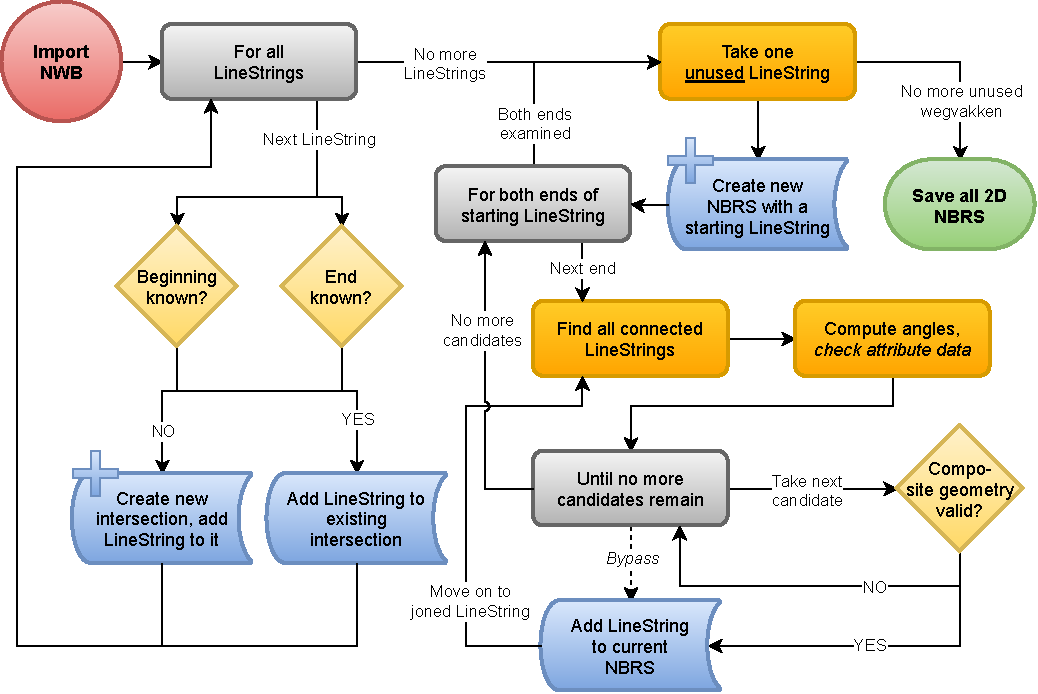
\includegraphics[width=0.9\linewidth]{final_report/figs/nbrs_generation.pdf}
    \caption{Flowchart-style illustration of the NBRS generation step of the pipeline.}
    \label{fig:nbrsgenerationflow}
\end{figure}

\subsubsection{Geometric algorithm}

This algorithm first creates a navigation structure from the input wegvakken. Each wegvak is a valid LineString, i.e. a connected series of line segments, which can be a few metres long, or even tens of metres long. From here on in this section, I will refer to wegvakken as LineString objects to make the description more general. The navigation structure is essentially a database that records which LineStrings of the road network start and end in which intersections. As this algorithm is not allowed to use the pre-made NWB intersections from the attribute table, intersections are defined by their coordinates (to one decimal). The navigation structure is based on hashing, hence it has good performance. The procedure consists of examining both ends of each input LineString and either creating a new intersection with it (if one does not exist at that location yet), or adding a reference to it in the intersection that is already found in the navigation structure. This is shown on the left in Figure \ref{fig:nbrsgenerationflow}.

The next step is to iteratively nucleate NBRS generation until no unclassified LineString objects remain. The algorithm takes one LineString, initialises an NBRS with it, and then attempts to extend it with further LineStrings on both ends to form an NBRS. First, recursive extension is initiated on the last vertex of the LineString, and once that completes, on its first vertex. The recursion examines the vertex, uses the navigation structure to find connected LineStrings and may connect one of them if certain conditions are met (see the next paragraph for the conditions) and progresses deeper into the recursion by doing the same with the LineString it just connected.

When the search for connected LineStrings succeeds, either a single one may be found, or multiple ones in case of a real-life intersection. If multiple candidate LineStrings were found, the algorithm needs to decide which one to connect based on a set of geometric conditions. First the angle between the last line segment of the previous LineString and the first line segment of all the candidate LineStrings are examined, and the continuation with the most optimal angle is selected (corresponding to the straightest possible continuation of the road). A composite geometry of the pre-existing NBRS and the new segment is then created and tested for self-intersections. If the composite geometry fails this test, the next best candidate is examined, and so on until a candidate succeeds, or the iteration runs out of candidates in which case the recursion terminates. When both recursions (going forward and backward from the LineString that nucleated the NBRS) finish, the NBRS is deemed complete and the next NBRS is nucleated. The self-intersection test is also performed when only one connected LineString is found.

\subsubsection{Semantic algorithm}

The semantic algorithm is built on the same framework as the geometric one. Most steps of the procedure are slightly modified equivalents of the ones in the geometric algorithm, hence I will here focus on describing the differences.

The navigation structure of the semantic algorithm is based on the JTE IDs (junctie IDs) found in NWB, which are unique identification codes belonging to each intersection of wegvakken in the dataset. Each wegvak possesses an end and beginning JTE ID, which are used to assemble the navigation structure in place of the coordinates in the geometric algorithm.

The nucleation of NBRS takes place in a similar manner to the geometric approach, but here each NBRS is associated with a specific wegnummer (road number) and BST code (a code related to the role of each road). LineStrings are only joined to an NBRS if they have matching road numbers and BST codes, which is what the text \textit{check attribute data} in the flowchart refers to. The candidates are still processed in the order or decreasing angle optimality, like in the geometric algorithm. However, the composite geometry needs not be checked for self-intersections, as roads satisfying the semantic conditions do not self-intersect in real life. This improves performance, as the intersection and validity checks of the resulting geometry is costly in terms of computational complexity. This shortcut is indicated by the dashed \textit{bypass} path in Figure \ref{fig:nbrsgenerationflow}.

\subsubsection{Challenges encountered}

I encountered three distinct issues while I was developing this part of the software. The first problem was that while NWB has a valid graph structure when one looks at its attribute table, the same graph structure is not always easy to derive solely from the geometry. While the semantic algorithm does not suffer from this problem, the geometric one does. Each wegvak has a pointer in its attribute table to the IDs of the two intersections it is connected to. This makes it possible to navigate the graph with minimal effort, but the underlying LineStrings may occasionally be disjoint (due to the coarse georeferencing NWB uses), in which case the software needs to "guess" which other LineString it might be connected to, if any. Fortunately, this was not difficult to implement using the coordinate-based navigation structure - reducing the decimal precision in it solved the issue in most places. A second issue was that the geometry of wegvakken often reverses in the middle of a valid series that might form an NBRS, requiring the implementation of a workaround especially in the code that computes the angles. Lastly, for reasons that have to do with external conditions that NWB needs to meet, motorway ramps are connected to motorway lanes at angles that do not reflect real-life geometry, occasionally causing the algorithm to merge ramps into motorway NBRS and vice-versa. A dedicated workaround was also necessary here, to recognise this situation and treat it correctly.

\subsection{Elevation estimation}
\label{sub:m_elevationestimation}

The elevation estimation stage of the pipeline consists of two operations. The first operation is to associate each NBRS vertex with a preliminary elevation estimate based solely on nearby Lidar points, and the second a refinement step to eliminate occlusion-related artefacts. The procedure is illustrated by the flowchart in Figure \ref{fig:elevationestimationflow}.

\begin{figure}
    \centering
    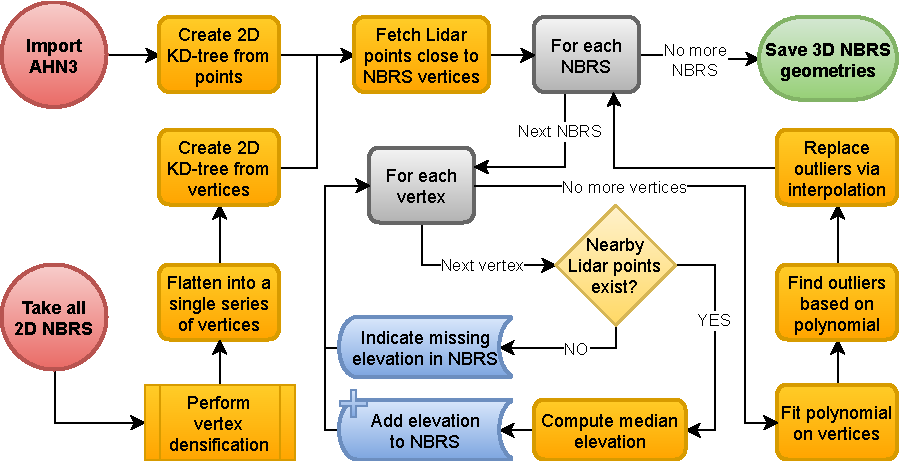
\includegraphics[width=0.9\linewidth]{final_report/figs/elevation_estimation.pdf}
    \caption{Flowchart-style illustration of the elevation estimation step of the pipeline.}
    \label{fig:elevationestimationflow}
\end{figure}

\subsubsection{Initial elevation estimation}

The process starts by importing AHN3, from where elevations will primarily be derived. It is assumed that this input is sufficiently small to allow in-memory use, i.e. that it is a cropped or clipped version of the full point cloud tile. Thus, this is the point in the procedure, where a global scaling solution would be most important. All other parts of the program work on the basis of processing subdivisions of the road network (NBRS or the underlying LineStrings themselves), which is already a good starting point for scaling.

The imported point cloud is first converted into a 2D KD-tree, so that area-based queries can be performed efficiently on it. This is followed by the flattening of all NBRS vertices into a single series, which was implemented in an effort to improve performance. Sending all vertices into the KD-tree query program at the same time as a flat list of vertices is far more efficient than performing the query individually for each NBRS vertex. This approach is reused in many subsequent parts of the implementation. Points closer than a certain threshold distance are fetched for each NBRS vertex. Before elevations are estimated, the flat list of coordinates is first split back into the discrete 2D profiles that NBRS represent. The median elevation of the nearby Lidar points of each NBRS vertex is then computed as a representative elevation estimate. Where too few points where found, the elevation is instead marked to be missing.

\subsubsection{Refining the preliminary elevations}

Following this step, each of the thus 3D-enriched NBRS are fed into an outlier filtering algorithm. The algorithm generates a distance series based on the horizontal coordinates of the NBRS, and fits a polynomial on these distances, and the elevation estimates. Since occlusion is almost always represented by short-wavelength data gaps or positive outliers in the Lidar data, these vertices will have considerable errors relative to the fitted polynomial. By interpolating values where outliers were detected and where elevations could not be obtained prior to this step, the quality of the preliminary elevations is improved considerably. The steps of this procedure are shown on the right in Figure \ref{fig:elevationestimationflow}.

The replacement values for outliers are interpolated \textit{linearly} based on the series of inlier vertices, i.e. they are not determined by the polynomial fit. The reason for this is, that it is not always possible to find good fits for NBRS using a fixed-degree polynomial, and while the polynomial model is always good enough to \textit{detect} outliers, its values are not conformant enough to replace them with. This polynomial-fitting approach is reused in various subsequent parts of the implementation.

The resulting coordinates now represent smooth 3D lines that preserve the input road network's 2D georeferencing, but which were enriched with elevations. These series are retained both as a list of vertices for the convenience of subsequent steps, as well as updated geometries of the original LineStrings that comprise the input road network. At this point, a preliminary 3D version of the road network can be written to disk.

\subsubsection{Vertex densification}

Although it is not strictly related to NBRS generation, vertex densification is not listed as a discrete pipeline step as it is a rather trivial operation conceptually. As a result, it is only presented in this report as a pre-processing operation of the present step of the pipeline. It is shown in \ref{fig:elevationestimationflow} as the first processing step that acts on 2D NBRS.

Vertex densification of the NBRS vertices refers to the operation of taking the wegvakken that make up each NBRS, and adding vertices to their line segments until no distance between vertices is bigger than a certain threshold. In my implemetation, this takes place as a recursive iteration. Each wegvak (LineString) of each NBRS is considered, and the densification algorithm is called on each line segment. The recursion consists of breaking the line segment in two halves if it does not comply with the threshold (a vertex is added in the middle), and then proceeding deeper into the recursion by doing the same with the two resulting halves. The densified geometries are assembled when returning from the frames opened by the recursion.

Like NBRS generation, vertex densification is done for the benefit of subsequent operations. Many operations - such as the present step - act on each vertex separately, gathering information related to the vertex from its AHN3 and DTB neighbourhood. Since the posting distance of AHN3 is far smaller than the line segments in NWB, increasing the density of NWB's vertices has practical benefits. It not only increases the resolution at which elevation can be estimated, but it also means that large-scale trends in the data will be represented more dominantly, i.e. algorithms will be better able to tell which parts of the road represent the road surface, and which ones are outliers due to occlusion. The practical benefits of this step were observed during development, and vertex densification was made an intrinsic part of various other parts of the pipeline too.

\subsubsection{Challenges encountered}

The main challenge encountered was that at the beginning of the algorithm, NBRS still consist of references to a series of wegvakken (LineString objects), but which then need to be flattened into a single series (for KD-tree queries). Thus, the problem regarding random reversals of wegvakken still stands, and a workaround needed to be implemented that rotates reversed wegvakken into the correct orientation during the flattening step. The correct orientation is always relative to the first wegvak in the NBRS. Needless to say, these then needed to be rotated back again into their original positions when writing the elevations into the source data, to avoid introducing changes to the 2D geometry of NWB.

A second challenge was to find a good benchmark of what to consider outliers after fitting polynomials. I needed to choose a metric that works well with all the typical types of occlusion-related artefacts that might show up in the data, such as overlying bridges of various heights, civil engineering structures of such bridges next to and above roads, motorway signs, tunnels, and so on. After experimenting with various approaches, I settled on one that involves computing the standard deviation of errors relative to the polynomial model, and then setting the threshold as a multiple of standard deviations (which is also in line with standard scientific practice). Below a certain absolute value of standard deviation, I artificially raise it to a set minimum level to avoid performing interpolation in road surfaces that are exceptionally smooth.

\subsection{Lidar segmentation}
\label{sub:m_lidarsegmentation}

The Lidar segmentation workflow is more complex than the two I described above, and some of the intricacies are omitted in the relevant flowchart (Figure \ref{fig:lidarsegmentationflow}) to keep its complexity manageable. I will attempt to fill in some of these details here in the text, referencing where approximately in the flowchart they occur.

\begin{figure}
    \centering
    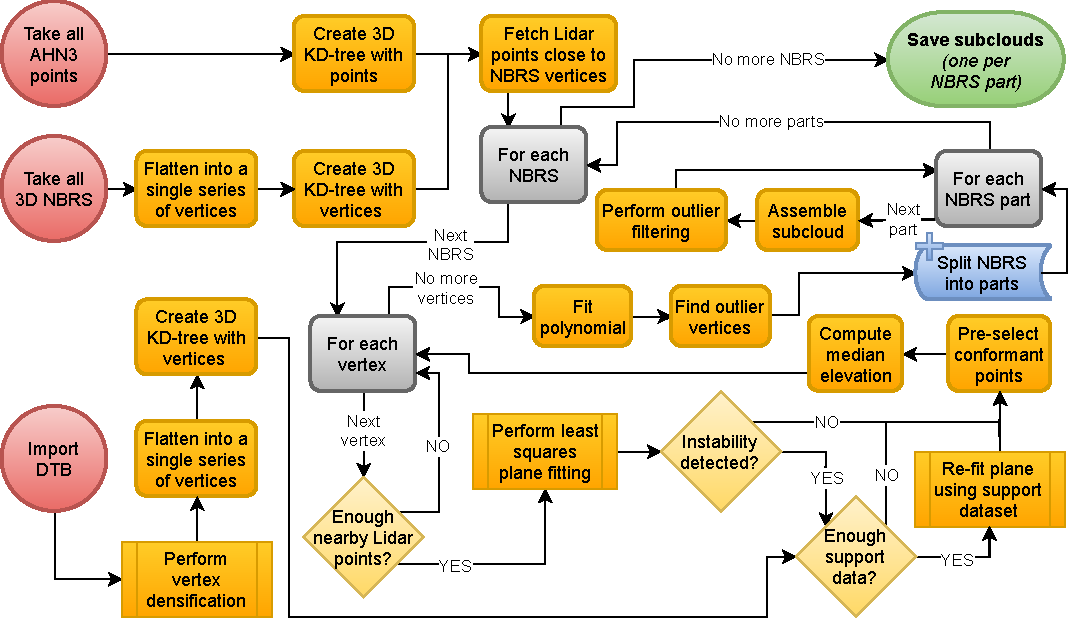
\includegraphics[width=0.9\linewidth]{final_report/figs/lidar_segmentation.pdf}
    \caption{Flowchart-style illustration of the Lidar segmentation step of the pipeline.}
    \label{fig:lidarsegmentationflow}
\end{figure}

\subsubsection{Preparation and plane fitting}

The program first creates KD-trees from the 3D point cloud, the flattened list of all 3D NBRS vertices, as well as a flattened list of all vertices found in the support dataset, DTB. Since DTB is a vector dataset that consists of 3D LineStrings, the lines are also vertex-densified prior to being converted into a point cloud and then into a KD-tree. The densification drastically increases the effectiveness of using DTB as a point cloud.

Much like in the preliminary elevation estimation workflow, a Lidar point cloud KD-tree query is performed as a bulk operation on each NBRS vertex (using the KD-tree made from the NBRS vertices). This results in "patch" of Lidar points being selected for each NBRS vertex with the underlying selection geometry being a sphere, rather than a 2D circle (as was the case in preliminary elevation estimation). This means that the relevance of the selected points will already be far more certain than before. However, each of these patches are further processed below to enhance the results.

The program then fits a plane on each patch of Lidar points using the least-squares method. Planes are only fitted if there are a set minimum number of points to support it, a threshold which is defined in terms of reaching a certain minimum point density inside the patch. If it is not reached, the points may still be passed on if a lower threshold is reached, in the hope that the support dataset (DTB) can re-position the plane to them in later parts in the algorithm and find some of them to be conformant with it. Below this second threshold, neither a fitted plane, nor the points are passed on. In the flowchart (Figure \ref{fig:lidarsegmentationflow}), this stage is shown in a simplified form which excludes the logical branch between the two thresholds, as it is insignificant.

\subsubsection{Refining plane fits and pre-selecting points}

Next, the program processes each NBRS starting from their first vertex and considering each vertex, one by one, in the order in which the vertices geometrically represent the road centreline making up the current NBRS. The program searches procedurally for places where the succession of fitted planes may indicate a break in shape of the surface. At the beginning of the iteration, the program first initialises a set of variables describing the \textit{previous} plane fit's relative position to the 3D NBRS centreline, the median elevation of the relevant patch's Lidar points, and the standard deviation of their distances to the fitted plane. By examining variations in these metrics (comparing always those of the current vertex and plane to the previous one), the algorithm can detect where the plane fits become unstable. Significant changes relative to the previous vertex and plane may indicate the presence objects occluding the sensor's view of the road's surface. I determined the exact metrics and parameters (thresholds) related to detecting instability based on experimentation and iterative refinement. The current setup works well with all testing datasets examined. This step is represented in the flowchart by the conditional element labelled "Instability detected?".

Originally, the algorithm was configured to automatically revert to the previous plane in case of plane instability and be allowed to use the reverted plane for a few iterations before asking help from the support dataset (in case the road emerged from underneath the occluding object after a few iterations). If the support dataset could also not help (due to e.g. a lack of coverage) after the expiration of the tolerance period, the algorithm would "give up" and move on to the next NBRS. This meant that long occluding objects and no DTB coverage could prevent the algorithm from processing certain NBRS, for instance ones containing tunnels.

\subsubsection{Handling breaks in the trend and missing data}

I eventually revised this algorithm to be more robust and to produce useful results even in a complete absence of a support dataset such as DTB. In the current version of the implementation, the algorithm is only allowed to attempt to use the previous plane \textit{once} before trying to use DTB. The point cloud generated from DTB contains road surface measurements only, so it can be relied on to provide "assistance" where AHN3 is ambiguous. If a previous valid plane exists, then DTB is queried for points relatively close to the previous valid plane (using the centroid of the points on which the plane was fitted). If not, then the centre of the query is the current NBRS vertex itself. If a reasonable amount of DTB points could be thus recovered, then the process is repeated by performing a second KD-tree query on the centroid of these DTB points, and the plane is then re-fitted onto the retuned points. The second query ensures that as many useful DTB points are included as possible. The program then assesses the distribution of Lidar points in the patch close to the re-fitted plane, and if the majority are found to be roughly conformant with it, then the plane is re-fitted a third time to make sure that in the end it is based on the Lidar points and not the support data wherever possible. The necessity of this last step will be reasoned in more depth in Section [REF], in a nutshell the reason in the case of my datasets was that in many places DTB is up to two decades older than AHN3, leading to significant, but locally consistent differences between the elevations suggested by the two datasets.

In the new version of the algorithm, the program does not declare failure if it is no longer allowed to revert the plane to the previous and find support data to also be unreliable or missing altogether. Instead, it simply relaxes its conditions and continues as though it were starting to process a new NBRS. This bypass allows the program to continue processing the NBRS even if it is aware that there was a noticeable shift in the position of the fitted planes, or a data gap. Artefacts due to such places are now handled separately, after the iteration has finished.

Each iteration of this algorithm finishes by looking at the final plane fit of the Lidar patch of the current vertex, and pre-selecting those AHN3 points which conform well with it. The median elevation of these points is also saved as it will be used in the next step. DTB points are also merged into this subcloud, but only in places were they were used to re-position the plane fit as described above.

The above iteration is shown as the loop labelled "For each NBRS vertex" in Figure \ref{fig:lidarsegmentationflow}. In the implementation, the nesting of the iterations in different, but this description is easier to understand and is fully equivalent to the implemented version in terms of what it achieves. The same is true about the top-level iteration ("For each NBRS" in the flowchart), which in the implementation is broken into several parts for programming convenience.

\subsubsection{Breaking NBRS into parts}

Once the last vertex of the NBRS has been processed, a post-processing procedure is executed before moving on to the next NBRS. Based on the median elevations which were saved during the iteration, the program once again has a new 1D profile which it can examine for outliers. Missing elevations in the series generally indicate that there is a data gap in both AHN3 and DTB there. On the other hand, outlier elevations almost always indicate that the plane fit was corrupted by an overlying features that caused occlusion or partial occlusion and it was also not possible to rectify the plane fit based on DTB. Instead of interpolating at these locations, the program generates a boolean mask. This boolean mask is then post-processed to eliminate short-wavelength changes and used to construct a list of intervals inside the NBRS that were found to be affected by neither of the above two problems. Thus, a further subdivision of the road network is introduced: \textit{NBRS parts}. Each part corresponds to an interval in its parent NBRS with reliable input coverage.

For each NBRS part, the patches are combined into a subcloud (including points which originate from the supporting dataset, in our case DTB). A quick outlier filtering step is applied to them eliminating all points in the subclouds which are isolated (have no neighbours within a certain distance). This is easy and computationally efficient to execute by converting the data into KD-trees and performing nearest-neighbour queries on them.

A hashed structure is initialised at this point in the program that allows the program to remember which points in the subclouds originated from the support dataset. The use of this structure is described in Subsection [REF] below.

As Figure \ref{fig:lidarsegmentationflow} shows, this concludes the point cloud segmentation procedure. Each NBRS part has its own subcloud, which are aggregated (but not merged) on the NBRS level and used in all subsequent parts of the program. The results can be written to disk as a LAS file, in which points are classified based on which dataset they come from, and which NBRS and NBRS part they belong to.

\subsubsection{Challenges encountered}

The above description already contains an account of how my methods relating to treating breaks in the trend and missing data evolved, and I will further elaborate here on this topic as it represents the biggest challenge encountered. While detecting small-scale variations in a range of metrics is not a difficult task in general, finding a set of metrics and corresponding thresholds universally applicable to all the data proved to be challenging. Furthermore, the simple approach of starting on one end of the NBRS and examining its vertices one by one eventually turned out to have insurmountable limitations. As it has no concept of global trends in the NBRS, it can only rely on its previous iterations to detect breaks in the trend. With the right configuration of metrics, I expected to be able to overcome this barrier, and wanted to keep this approach also because it allowed me to make use of DTB in an effective, elegant manner.

However, I eventually realised that this approach has another limitation: in regions with outlying or missing AHN3 data and no DTB coverage \textbf{and} a change in the elevation of the road, the iteration would lose its references and not be able to continue after the road emerged at the changed elevation. This limitation only manifested itself in places where NBRS contain long tunnels. Furthermore, keeping regions with no coverage inside NBRS also meant that in subsequent steps, I was optimising contours and continuing the road surface model TINs across them as well - sometimes over tens of metres or more. This turned out to be problematic especially with active contour optimisation, which frequently ended up producing corrupted outputs as a result.

To solve all these issues, I extended this part of the implementation with methods to examine the global trend represented by pre-selected points after the procedural iteration. This is where I transitioned to first saving Lidar patches per vertex separately (instead of adding them straight to the subcloud), constructing a polynomial based on their centroids to describe the overall trend, and detecting areas where the points lay above the expected road elevation (converting these into no-data regions). Then, all I had to do is break NBRS into parts where such no-data regions begin and end, and propagate these changed to all the subsequent parts of the pipeline. As this step takes care of outlier planes where no DTB coverage is available, the role of the procedural iteration was reduced to managing DTB-based filling of holes, it no longer tries to eliminate outlier patches on its own, where DTB is unavailable.

\subsection{Edge approximation}
\label{sub:m_edgeapproximation}

The generation of preliminary edges is based on identifying edge points at discrete intervals in the road centreline (on each vertex, including ones created during vertex densification). The procedure takes place on the level of NBRS parts, and it is illustrated in Figure \ref{fig:edgeapproximationflow}.

\begin{figure}
    \centering
    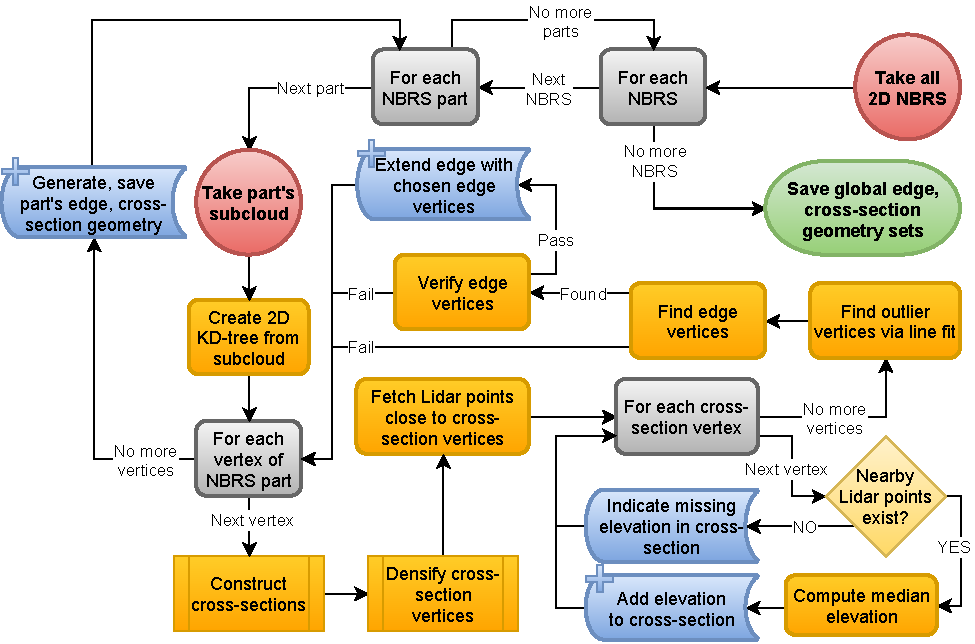
\includegraphics[width=0.9\linewidth]{final_report/figs/edge_estimation.pdf}
    \caption{Flowchart-style illustration of the edge approximation step of the pipeline.}
    \label{fig:edgeapproximationflow}
\end{figure}

\subsubsection{Constructing edge point candidates}

First, the subcloud of each NBRS part is used to create a 2D KD-tree. 2D suffices here, because it is a reasonable assumption to make at this point that the subclouds of NBRS parts no longer have a significant number of points that would not describe a 2.5D surface (e.g. reflections from occluding objects). On each vertex of the NBRS part, a cross-section is then constructed. Cross-sections are built roughly orthogonal to the centreline locally, their azimuths are based on the mean azimuths of the two line segments that contain the given vertex (except for the first and last vertices, which are simply based on their single parent segment's azimuth). The cross-sections are densified considerably and their densified vertices' are then flattened into a single list and used in a bulk KD-tree query. Lidar points very close to the vertices are thus fetched, and their median elevation is saved as the elevation of the given vertex. This step works on a small, sub-metre scale, meaning that using the native density of AHN3 (no thinning applied) is particularly important from here on.

Each cross-section then represents a 1D profile, elevations against distance from one end to the other (with the NBRS part's vertex in the middle). Each of them is fitted with a line and outlier vertices are identified based on the model line. The program then tries to find suitable edge points among the inlier cross-section vertices, on both sides of the NBRS vertex in each cross-section. Together, these points will form the preliminary edges. In each of the cross-sections, the program starts from the outermost cross-section vertex and progresses inwards. Once a certain consecutive number of inliers is encountered with no outliers in-between them, the program assumes having reached the road surface and flags the current vertex as the edge vertex.

The full length of each cross-section, which is a constant parameter, represents the maximum road width the program can work with. The optimal value of this parameter depends on the permitted road dimensions in the given road network (AHN3 in our case), and it lies in a rather narrow band. If it is too small, the preliminary edges may lie far inwards from the real-life edges, and exclude large portions of the real-life road surface as a result. If it is too large however, false positive hits outside the real-life road surface will corrupt the preliminary edges, especially where roads are thin and other smooth surfaces are found in their surroundings.

\subsubsection{Enforcing constraints}

Flagged vertices are only accepted as edge vertices if they also pass a range of further conditions relating to the minimum width, as well as sudden elevation changes and road width changes. The minimum road width is enforced for each pair of edge points individually. However, much like in the first part of the Lidar segmentation step, the latter two are checked by comparing the metrics of the current edge point candidates to a previous few. Only if this verification procedure succeeds, does the program extend the NBRS part's preliminary edges with new vertices.

In areas where the above procedure fails multiple times consecutively, "gaps" are created in the preliminary edges. These are not real gaps in the sense that the last pair of edge points before the gap, and the first pair after, are still connected in the output - it simply means that the lengthwise sampling is coarser locally. Compared to the artefacts that would appear in the absence of the above threshold enforcement procedure, small gaps are an acceptable compromise, especially if the NBRS were sufficiently vertex-densified prior to this step. However, long gaps cause various problems in later pipeline steps. To avoid creating long gaps in the generated edges, a relaxation of the conditions takes place after a set number of failures. After relaxing the conditions, the first inlier point is selected when fitting the next cross-section with a line, and the constraint regarding sudden changes in width is also ignored. Immediately after a success, the constraints are re-enabled. This temporary relaxation allows the algorithm to regain its reference even if a sudden real-life change in the road's width is encountered, and also helps in scenarios where the location of the edge is ambiguous.

Lastly, once per NBRS part the program generates the final 3D cross-section and edge geometries and saves them. After all NBRS parts have been processed, the global cross-section and preliminary edge object is also created. This can be written to disk as a Shapefile to visualise the results.

\subsubsection{Challenges encountered}

Originally, this step was going to be a preparatory step for the sole purpose of providing initial edge shapes for the active contour optimisation algorithm. I first implemented it almost exactly to the specifications found in the P2 document. However, it soon became clear that better active contour optimisation results require better preliminary edge estimates, and thus I implemented a range of tweaks and improvements. It appeared that the best active contour optimisations corresponded to where the preliminary edges were on the road surface, slightly inwards from the location of the real-life road edges. This is what defines the final implementation of picking edge point candidates - the program starts from the outer edges of the cross-sections, and progresses inwards until it can safely conclude that is has already been inside the road surface for at least a few vertices.

A further challenge corresponded to the point in development when I decided to make active contour optimisation optional. I needed to implement modifications to these methods to allow preliminary edges to be used for TIN construction directly, at the same time still maintaining compatibility with active contour optimisation. This is what resulted in the addition of the system of constraint enforcement and constraint relaxation that takes place right before accepting a pair of edge point candidates. The main reason why this is beneficial for TIN construction is that it ensures that the edges do not have a zero (or very tiny) width anywhere, and that it reduces the chance of road widths being overestimated. The former ensures that there is always a non-zero area on both sides between the underlying road centreline and the corresponding preliminary edges, in turn ensuring the possibility to select Lidar points in these 2D areas in the TIN initialisation step. The latter decreases the chances of including off-road points in the road surface models, both during TIN initialisation and extension. For more information about the TIN construction phases, please refer to Section \ref{sub:m_tinconstruction}.

\subsection{Active contour optimisation}
\label{sub:m_activecontours}

The optimisation of preliminary edges is based on constructing one attractor map for each NBRS part, and running active contour optimisation to attract the preliminary edges to certain features in the attractor maps. The procedure is illustrated in Figure \ref{fig:edgeoptimisationflow}.

\begin{figure}
    \centering
    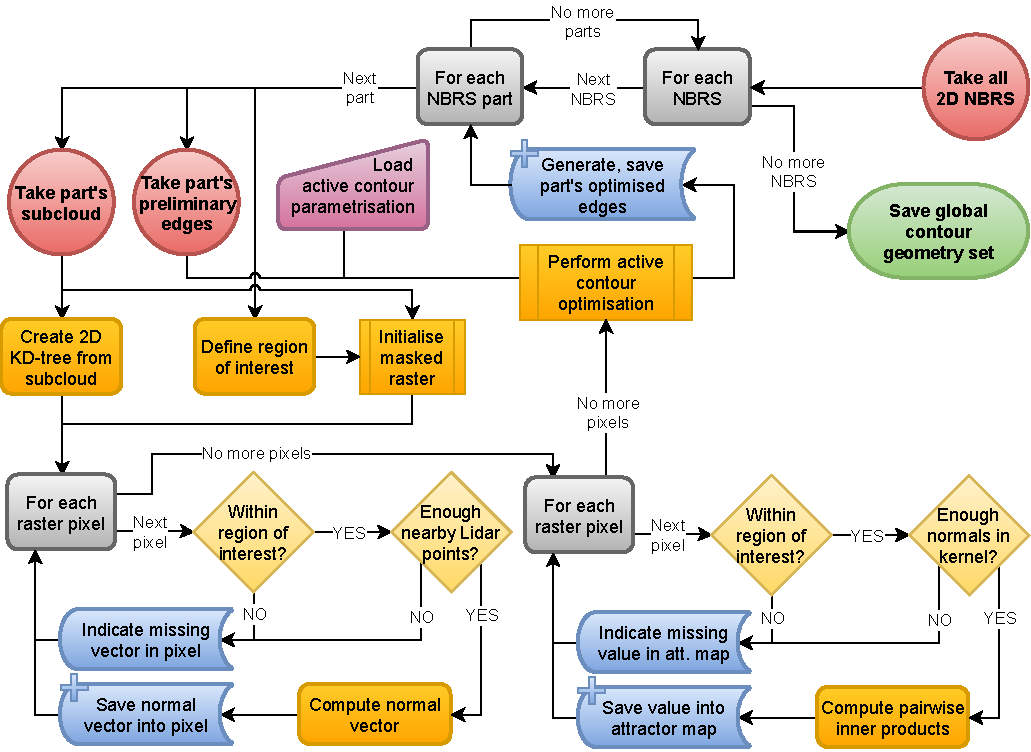
\includegraphics[width=0.9\linewidth]{final_report/figs/edge_optimisation.pdf}
    \caption{Flowchart-style illustration of the active contour optimisation step of the pipeline.}
    \label{fig:edgeoptimisationflow}
\end{figure}

\subsubsection{Attractor map generation}

The procedure underlying this step is once again based on a 2D KD-tree of the subcloud of the NBRS part. 2D suffices because the underlying data structure of attractor maps are 2D rasters, and once again, because we are safe to assume at this point that the subclouds of NBRS parts no longer have a significant number of points that would not describe a 2.5D surface. When initialising the raster that underlies the attractor map, a region of interest is first derived by buffering the centreline by a certain amount. The rectangular-shaped raster is then masked out everywhere except for pixels whose centres lie within the region delineated by the buffer polygon.

The centre of each unmasked pixel is then used in a bulk KD-tree query to find a small 2D patch of nearby Lidar points. For pixel centres that have a sufficient amount of neighbouring Lidar points, a normal vector is computed. These normal vectors are computed as the normal vectors of the local plane fits of each such patch of Lidar points, and the least-squares-based approach is re-used in my implementation (from the Lidar segmentation step of the pipeline).

Normal vectors can be stored in the pixels in my framework, but they cannot be used directly in active contour optimisation because it requires scalar pixel values. To derive scalar values from the vectors, I designed a kernel-based approach in which the pairwise inner products of the normal vectors of all pixels falling into the kernel are computed and their median is taken. Since computing inner products is computationally expensive, not all combinations of the normal vectors in the kernel are dotted, only a representative random subset.

\subsubsection{Running the optimisation algorithm}

All parts of the above procedure take place in a temporary coordinate system which is defined in terms of the number of pixels in the X and Y dimensions from the top left corner. Before the preliminary edges can be overlain on the attractor map, they each need to be transformed into this coordinate system via scaling and translating their coordinates. Together with the attractor maps and a suitable parametrisation, the preliminary edges are now ready to be optimised. The optimisation algorithm is run separately for the edges on the two sides of the centreline, and the output optimised edges are then assembled into a single polygon (the NBRS part's contour). Lastly, the global collection of contours are assembled into a single object which can be written to disk to visualise the results.

The scikit-image implementation of active contour parametrisation is based on the original paper in which this this method was first described scientifically: \cite{kass_etal_1988}. In addition to taking the attractor maps and the preliminary contours as input, it also takes a set of parameters that can be tweaked to manipulate aspects of the optimisation. The most important aspects for us in this project are contour smoothness, attraction to brightness, attraction to edges and the total number of allowed iterations.

In Section [REF] I describe the recommended values for each of the variables, based on the fine-tuning I carried out as part of implementing this step. Here, I will describe the aims I had in mind while fine tuning. Firstly, the $\alpha$ parameter is set to zero in order to prevent the contours from contracting. Shrinking the contours lengthwise is not desired, as it needs to extend all the way to the two ends of the underlying NBRS part. Medium smoothness is desired because based on the testing I have done, this is one task in which active contour optimisation excels, it can smooth preliminary edges in a way that can eliminate small-scale protrusions that are generally meaningless, and can thus be considered noise. Importantly, I was unable to make use of the ability of active contour optimisation to take into account brightness. The attractor maps that I described above have a sharp contrast between the brightness of off-road pixels (which are dark), an road pixels (which are bright). However, this contrast is not localised to the edges of roads, hence any amount of attraction to either region would draw the contour deeper into that region rather than keep it on their boundary. Attraction in my recommended parametrisation is controlled entirely by edge detection, as this works correctly with my attractor maps. In terms of iterations, I decided to work solely with a maximum number of iterations rather than reaching a certain boundary condition. Setting a boundary condition terminates the optimisation process when the contours no longer move significantly in each step. Unfortunately, letting the contours evolve to this point results in the drastic enlargement of artefacts, as well as an unacceptable increase in computational complexity - I found iteration limits between 100 and 5000 to be the most effective, with each iteration being permitted to move the contour by up to one pixel only.

\subsubsection{Challenges encountered}

In terms of the first version of my implementation, the main challenge here was the trial-and-error nature of getting active contour optimisation to perform acceptably for the wide range of input geometries and attractor map features that are possible in our national datasets. I needed to refine the parameters of the optimisation algorithm needed to work well with the input data, but since I was also producing the input data myself, I was also in the position to fine-tune that in turn. As a result, the task was a joint fine-tuning procedure involving all prior steps in the pipeline leading up to this point, as well as the arguments in the algorithm's API. Of all the aspects of the input data that I tried to optimise, I invested the greatest amount of effort in pre-processing the attractor maps to bring out the the road edges in them as sharply as possible. I tried various moving-window techniques such as many types of edge detection, edge enhancement, blurring, as well as morphological operations such as dilation, erosion, opening, closing, and many combinations thereof. Sadly, I eventually concluded that none of these operations can achieve a noticeable improvement in the results, with the kernel-based normal vector attractor map and the native edge detection of active contour optimisation still producing the best results after several days spent on this.

Making matters worse, I found active contour optimisation to work only at high raster resolutions, with a pixel size around 0.5 metre typically producing the best results overall. Unfortunately, computational complexity grows non-linearly with decreasing pixel size, making debugging and fine-tuning very difficult, as well as putting the usefulness of such an algorithm into question considering the scale of the input data.

A further problem I found is that there are occasional small-scale features in the input data that tend to confuse active contour optimisation. Even for relatively short iteration lengths, such small artefacts may unpredictably corrupt entire NBRS part contours. For instance, small Lidar gaps due to stationary vehicles frequently overlap with the region where the road edges are suspected to be found. Active contour optimisation has no concept of no-data pixels, and reacts unpredictably to these holes regardless of what one uses as filling values. Another similar issue is that road edges are often characterised by sudden slopes beyond their edges, but with further flat regions beyond them. These slopes are often short, and their intersection with the off-road flat zone creates a second contrast in brightness that active contour optimisation may confuse with the real road edge. These features and other similar types of features frequently draw the contours further from the road than what would be acceptable to accurately classify Lidar points within the contours as road reflections.

Lastly, the effectiveness of the method is also far too reliant on the accuracy of the preliminary edges. The algorithm is sensitive to even the smallest of blunders in preliminary edge detection, and is also prone to fail in no-data regions. After I implemented the code to split NBRS internally into parts where longer regions suffer from the absence of data, part of this issue was solved, but another remained: where DTB is available but not AHN3, preliminary edges tend to shrink significantly, which often corrupts the optimised edges.

While my implementation works and produces usable results, its ineffectiveness an unreliability prompted me do make it possible to bypass its use in the software. This required modifications to various preceding steps of the pipeline, as well as all subsequent ones - a significant challenge. This bypass in turn puts into question the relevance of much of the pipeline structure, many parts of which were intended to lay the groundwork for active contour optimisation, and to make use of its output. I elaborate on this topic further in Section [REF].

\subsection{TIN construction}
\label{sub:m_tinconstruction}

As I emphasised in the previous section, various aspects of active contour optimisation were found to be lacking. The severity of the issues with this step prompted me to develop TIN construction in a way that enables it to function without active contour optimisation. Bypassing  the active contour optimisation step alters the requirements that the TIN construction algorithm needs to satisfy. In my planned pipeline, I made the assumption that points falling within the area of contours could be safely considered road points, and that conditional insertions would primarily be used to filter out obvious outliers. Working with preliminary edges (as well as \textit{inaccurate} optimised edges) necessitates a less straightforward, but more robust implementation that is capable of recognising outliers on a much smaller scale. The result is an algorithm that borrows ideas mainly from region growing and ground filtering algorithms. In in-depth explanation of the algorithm is found below.

The outermost iteration loops over NBRS, and NBRS parts are iterated one level below. In Figure \ref{fig:tinconstructionflow} this is explicitly indicated as iterating over NBRS IDs and NBRS part IDs respectively. In contrast with previous steps in the pipeline, the centrelines themselves are no longer used, hence the change in notation. 

\begin{figure}
    \centering
    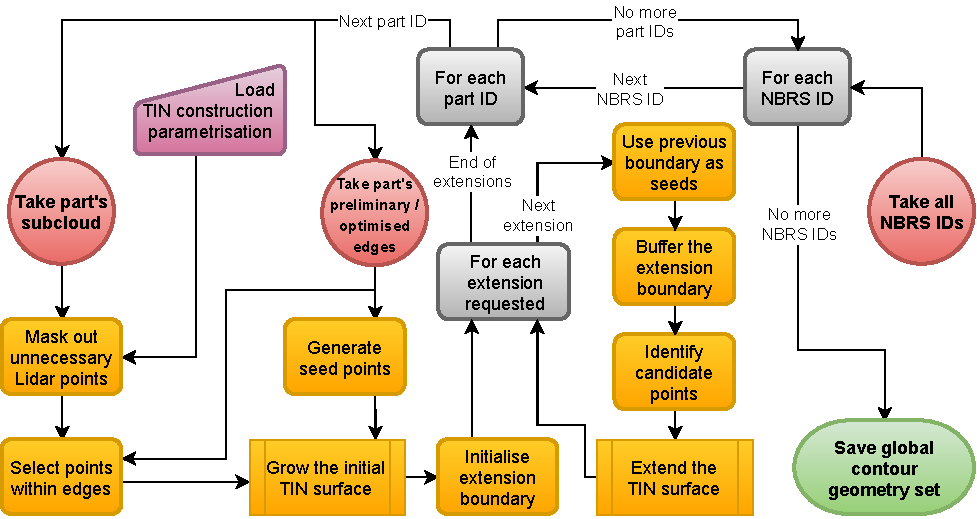
\includegraphics[width=0.9\linewidth]{final_report/figs/tin_construction.pdf}
    \caption{Flowchart-style overview of the TIN construction step of the pipeline.}
    \label{fig:tinconstructionflow}
\end{figure}

\subsubsection{Preparation for TIN initialisation}

Based on the parametrisation, the outermost boundary within which points will be considered for insertion (including TIN extension) is constructed as a polygon, and points falling outside of its interior are excluded from further consideration. Then, either the preliminary edges or the optimised edges are fetched for the given NBRS part. Since they are almost identical structurally, they can be treated the same way for the most part. They are used for two tasks: firstly, to construct a line halfway between the two edges to form the basis of seeding the TIN initialisation procedure, and secondly, to select points that fall within the edges as insertion candidates for the TIN initialisation step. This step is labelled "Grow the initial TIN surface" in Figure \ref{fig:tinconstructionflow}, marked as a pre-defined procedure because the underlying procedure is fairly complex. To keep the complexity of the flowchart manageable, both the TIN initialisation step, and the TIN extension step of this step are illustrated in a separate diagram, which is shown in Figure \ref{fig:tinconstructiondetailsflow}.

\subsubsection{TIN initialisation}

TIN initialisation refers to the process of constructing an initial, conservative approximation of the road surface. As I noted above, it considers those Lidar points only, which fall between the preliminary or optimised edges. It first looks up those Lidar points, which are very close to the seed points. As these points are all but guaranteed to fall on the real-life road surface, they are unconditionally inserted into the TIN and are then pushed on a stack that in this case I will refer to as the "buffer". At this point in the algorithm, as Figure \ref{fig:tinconstructiondetailsflow} shows, we leave the "TIN initialisation" group of operations and enter the "TIN growing" group (which is shared with "TIN extension"). The boundary vertices are also inserted into the TIN at this time (at an elevation of zero), which guarantees that the program can identify situations in which it is working with a triangle that touches the boundary.

At this time, the TIN contains a high density of small triangles in the immediate vicinity of the original centreline of the NBRS part. Furthermore, it contains large triangles connecting this area with the boundary inside of which the road surface is allowed to grow. During the initialisation stage, this boundary is represented by the preliminary edges or optimised edges themselves. Inserting these in the TIN serves a dual purpose. Firstly, it avoids raising errors when a conditional insertion test is being performed outside of the convex hull of inserted Lidar (and DTB) points. The boundary itself becomes the convex hull during the initialisation step, so each time the program tries to locate the triangle into which a given point would be inserted if it passed the test, will be guaranteed to succeed. Secondly, since the boundary is at an elevation of zero in the TIN, the program can easily identify when it is \textit{growing} the Lidar-defined surface rather than just inserting into a triangle already defined by three points from the subcloud. It also allows the program to be aware of the position of the tested point relative to the detailed surface and the boundary.

The buffer at this point consists of all the seed points that were inserted unconditionally. The buffer is fed into a KD-tree query over all the candidate points (points between the edges) in a bulk operation, and is then emptied. All points returned by the query are pushed on a stack, and this stack forms the basis for the conditional insertions. One by one, points on this stack are popped, and are conditionally inserted into the TIN. Figure \ref{fig:tinconstructiondetailsflow} does not describe the conditions themselves, but I will go into detail about them here.

First, the triangle containing the popped point is located. If the triangle is defined by subcloud points, then the elevation of the point according to the triangle is interpolated and the the difference in elevation is treated as an elevation discrepancy to which a threshold applies. If the threshold is not violated, then the distances to the three vertices of the triangle are computed, and based on that, the angles between the triangle's plane and the line segments connecting the popped point to the three vertices are also calculated. If any of the three angles violate a pre-set threshold, the point is not inserted.

If the located triangle contains one or more boundary points, the elevation discrepancy is computed in a different way. Growing the TIN needs to be done with some caution, as introducing erratic points around the edges of the current convex hull would entail that future insertions would have an incorrect basis for the conditional insertions and as a result, the surface would occasionally be allowed to grow in diverging directions. To minimise the chances of this happening, growing the surface takes into account multiple pre-existing TIN triangles in the neighbourhood, not just the closest ones. Specifically, all triangles containing the non-boundary vertices of the located triangle are fetched. Then, this is repeated with all the vertices of the resulting set of triangles. The vertices of this collection of nearby triangles are then fitted with a plane (re-using, once again, the least-squares method), and the distance of the tested point to the plane is taken to be a good approximation of the elevation discrepancy. Points in the buffer are always close to the pre-existing Lidar points in the TIN (see below for the reason), hence this is a reasonable assumption. The angle-based test is then administered the same way as for regular insertions.

Each popped point that ends up being inserted into the TIN is also pushed onto the buffer, which was previously emptied after it had been used for the KD-tree query to fill the stack. Once the stack becomes empty, the procedure restarts by performing another KD-tree query using the buffer, and refilling the stack with new points to insert conditionally. In other words, as long as points are being inserted, and these points have uninserted subcloud neighbours, the procedure will repeat. The buffer and the stack are kept separate so that KD-tree queries can be performed periodically as bulk operations, rather than individually - this is more efficient computationally.

As soon as no more insertions are taking place, the iteration ends and returns all points inserted into the TIN, in the order they were inserted. The TIN itself is not kept, instead it is reconstructed later on - this is due to the fact that point deletions in the triangulation package "startin" do not appear to work reliably, but we do not wish to keep the boundary points in the TIN. The straightforward way to achieve this without point removal is by reconstructing the TIN with the subcloud points only, keeping an external track of insertions to make this possible.

\subsubsection{TIN extension}

The extension of the TIN takes place in an iterative manner. The implementation accepts arguments that set the amount by which the boundary should be buffered in each iteration, as well as the number of extension iterations (steps). The starting boundary is \textit{not} the same as the one used during initialisation of the TIN. There, the preliminary or optimised edges were used, but here the first iteration's boundary is buffered from the seed line (the line halfway between the preliminary or optimised edges). This allows the algorithm to take another look at the points between the edges in case in missed any good candidates during initialisation.

The seeding of extension iterations is different than that of the initialisation step. The seed points are always derived from the boundary used in the previous iteration. Furthermore, in TIN initialisation the candidate points included all points between the road edges, whereas in the extension steps only the points located in 2D between the previous and the current boundary, are considered. Depending on the parametrisation, the boundary may be buffered to examine areas beyond the preliminary or optimised edges, which is the main point of the extension phase. It allows the program to grow the surface into areas which were not between the edges because of imperfections in how the edges were generated. It is, in a way, a means to counteract the phenomenon of the road surfaces getting very thin where edge detection or optimisation underestimated their width.

Each iteration first reconstructs the TIN yielded by the previous iteration, and inserts its new, buffered boundary into it. Boundaries are always at zero elevation, hence when the previous iteration's boundary is reused to seed the current iteration, it first needs to be \textit{transposed to 3D}. This is done by creating a KD-tree from all pre-existing TIN points and associating the closest one's elevation with each vertex of the seed geometry. It is then ready to seed the new iteration by itself being the basis for KD-tree queries on the new candidate points. However, the results of this query are not inserted into the TIN unconditionally, like they were in TIN initialisation. Instead, they are simply pushed to the buffer to start the main iteration involving the conditional insertions. The assumption that points close to the seed geometry are sure to be part of the real-life road surface no longer applies, as the seed geometry in extensions may be far from the centreline depending on what stage of buffering it is in.

Once TIN extension has finished, the final TIN is reconstructed and is saved. Thus, one TIN object per NBRS part is saved, and these are not merged or joined together into a single TIN in any way. My implementation offers the possibility to write these TINs to disk, each one in a separate OBJ file. The algorithm automatically filters out triangles with areas and circumferences large enough to indicate that they cannot be relevant to the road surface.

\begin{figure}
    \centering
    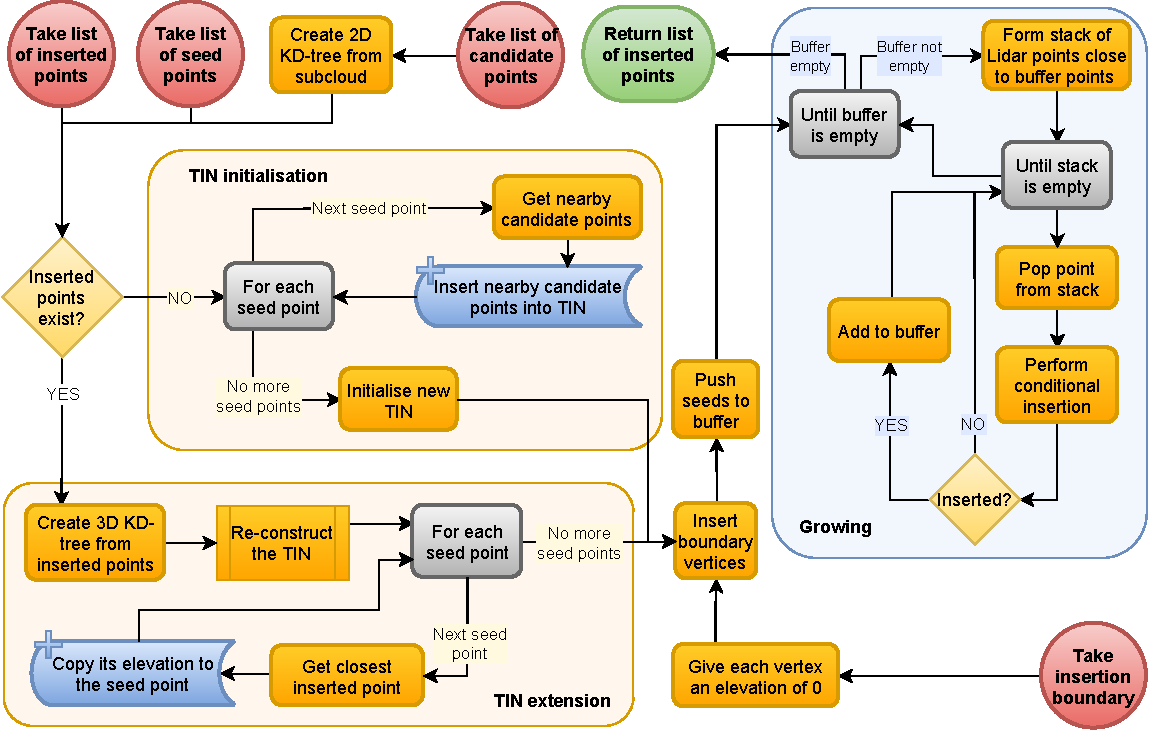
\includegraphics[width=0.9\linewidth]{final_report/figs/tin_construction_details.pdf}
    \caption{Flowchart-style illustration of the details of the TIN construction step of the pipeline.}
    \label{fig:tinconstructiondetailsflow}
\end{figure}

\subsubsection{Challenges encountered}

As implementing such a complex algorithm in this pipeline step was not originally intended, the biggest challenge here was to come up with a good solution within the timeframe reserved for the project. In terms of the methods themselves, I spent the most amount of time and effort on developing a solution that allows the road surface to grow into regions not covered by the preliminary or optimised edges. While in all cases, the surface generated by TIN initialisation is adequate to generate 3D-NWB, my desired was to not only model the central, traffic-occupied part of the road, but to grow it to the real-life edges of the paved surface as best as possible.

I initially wished to build the TIN as a single growing operation, but this proved to be prone to spreading into off-road regions. Depending on what order certain groups of points are examined in, even sharp breaks in the underlying surface may appear smooth. A good way to deal with this problem would have been to decrease the query radius used in the buffer queries, but this in turn often prevented the TIN from growing at all. This is the reason why I eventually implemented the final version of the method as a combined operation of first initialising a conservative TIN, and then extending it iteratively by examining thin layers of additional points progressing outwards from the centre of the road.

Performing conditional insertions outside of the convex hull of the pre-existing TIN points was a challenge, as shown by the complexity of the implementation. Interpolation in the triangles is not available here, but the importance of assessing the compliance of the tested points with the neighbourhood is ever so important, if not more - it depends on these surface growing insertions, whether a TIN might accidentally spread into an off-road area, or not. The final approach appears to work well in most scenarios, with the worst performance exhibited in regions where the road edges are slightly off road, causing off-road points to be present already in the conservative initial TIN surface.

Various other challenges were encountered during the development of this step, and some remain unsolved. More details about this topic are found in Section [REF].

\subsection{Interpolation in TIN and snapping}
\label{sub:m_interpolation}

\subsubsection{Interpolation and origin tracking}

This is the last step in the pipeline, and its primary purpose is to use the TINs generated in the previous step to enrich the source road network with the final elevations. As Figure \ref{fig:elevationinterpolationflow} shows, the first step in this procedure involves iterating through all NBRS parts, and performing the interpolation step itself. In rare cases, it is possible that an interpolation will fail, which depends on how well-behaved the relevant preliminary edges or optimised edges are (described in more depth in Section [REF]). For vertices where the interpolation succeeded, the interpolated elevation is written into the vertex.

An additional step takes place during this iteration. To make it possible to keep track of which elevations come from where exactly, the algorithm recognises triangles that have vertices that originate not from the AHN3, but from the DTB. Before performing the interpolation, the triangle in which the interpolation will take place is fetched, and the origin of its vertices is examined. If none of them are from AHN3, the origin of the elevation is deemed to be DTB. If one or more of the vertices are from AHN3, the origin is marked to be AHN3. For simplicity, the algorithm does not explicitly indicate what mixture of AHN3 and DTB vertices were found in the triangle. These are used in the accuracy estimation step, please refer to Section \ref{sec:m_accuracyassessment} below for the details.

The implementation uses linear interpolation in the TINs. This is one of the simplest interpolation techniques available for TINs, and it is also the one most widely studied among them in the literature I studied (see Section \ref{sec:lidaraccuracy}). It is particularly suitable to this research, because its error propagation formulae are are readily available in the literature, and because an implementation of it forms part of the \textit{startin} package which I use to build the TINs and interpolate in them. It interpolates using barycentric position of the point where interpolation is desired. The closer it is to one of the vertices of the triangles, the bigger the vertex's influence becomes on the interpolated elevation. If it is closer to the centre of the triangle, the influence of the vertices is more evenly distributed.

\subsubsection{Vertex snapping and gap filling}

The next step is to perform vertex snapping at intersections. TIN surfaces close to intersections are expected to be comprised of roughly the same vertices, hence the assumption is made that snapping intersection vertices together will not introduce abrupt elevation discontinuities. The procedure, which is performed for each NBRS, consists of taking each vertex one by one, and constructing a hashed representation of their 3D positions. If a point is already found to exist in the hashed storage, its elevation is snapped to that which already exists. Since self-intersections of NBRS are not possible, if such a point is encountered, such a match necessarily represents a location where \textit{another} NBRS ends or begins - in other words, a real-life intersection.

Due to NWB's coarse georeferencing (often only one decimal or no decimals), checking 2D matches of coordinates is not enough. Each time a match is found, vertical distance is also examined prior to snapping, to avoid blunders that could be caused by snapping together vertices that are at perfectly matching 2D coordinates, but which in fact belong to roads that are in a non-intersecting 3D relationship (one passes aobve the other).

The last step of the procedure is to infill gaps left by failed interpolation. Such gaps may be present due to small-scale inaccuracies in the preliminary or optimised edges, or due to the lack of primary \textit{and} secondary data at the same time. In such blind spots, NBRS are generally split into multiple parts, but this step again treats the entire NBRS as a single 2D profile. Vertices found between NBRS parts have no underlying TINs and no elevations as a result. These gaps are filled using simple interpolation, and instead of indicating their origin as either AHN3 or DTB, it is recorded to be the result of such interpolation. The technique is governed by the formula

$z_{p} =
\begin{bmatrix}
x_{pt}\\
y_{pt}\\ 
1
\end{bmatrix} =
\begin{bmatrix}
 a_{0} & a_{1} & a_{2} \\
 b_{0} & b_{1} & b_{2} \\
 c_{0} & c_{1} & c_{2}  
\end{bmatrix}
\begin{bmatrix}
z_{0}\\
z_{1}\\ 
z_{2}
\end{bmatrix}$

where $x_{pt}$ and $y_{pt}$ denote the X and Y coordinates of the location of interpolation (inside the triangle), the matrix in terms of $a_{0}$ to $c_{2}$ contains terms dependent on the 2D geometry of the triangle, and where the last vector corresponds to the three elevations of the three vertices of the triangle. Lastly, $z_{p}$ is the interpolated elevation. Please refer to \cite{fan_etal_2014} for the expressions for $a_{0}$ to $c_{2}$.

\subsubsection{Outputting 3D-NWB}

The last step of the pipeline converts the internal road centreline data structure of the program (NBRS parts and NBRS) back into the data structure used by the input data, which are the LineStrings that are called wegvakken in NWB. In effect, the 2D geometry of each input LineString is overwritten with the new 3D geometry created using the original 2D coordinates, and the newly generated final elevations. Unlike at the end of preliminary elevation estimation (see Section \ref{sub:m_elevationestimation}), the original orientations of wegvakken is automatically respected irrespected of some of them having been internally flipped, because the elevations are mapped from the dictionaries (based on 2D coordinates) directly into the geometries. The origins of the vertices and the accuracy estimation data are not written into this file, as arrays are a type of data that cannot be stored in the attribute table of a Shapefile. This data can be viewed inside the program, or written to disk as CSV files.

\begin{figure}
    \centering
    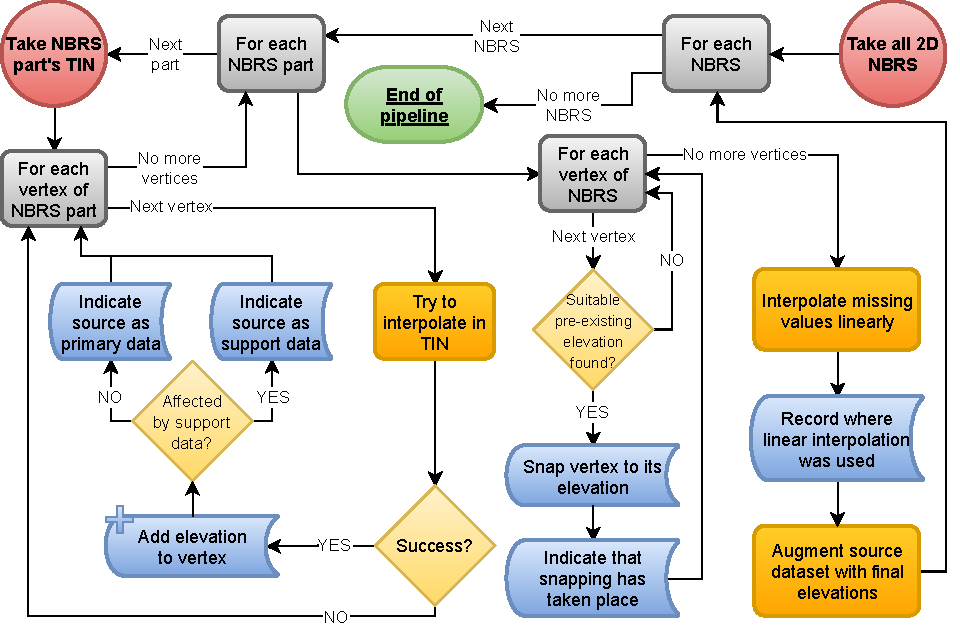
\includegraphics[width=0.9\linewidth]{final_report/figs/elevation_interpolation.pdf}
    \caption{Flowchart-style illustration of the elevation interpolation step of the pipeline.}
    \label{fig:elevationinterpolationflow}
\end{figure}

\subsubsection{Challenges encountered}

As the tasks carried out in this pipeline step are relatively trivial, all challenges encountered were equally simple to solve. The only part of the implementation that proved to be less straightforward was the tracking of the origin of vertices through the TIN-based interpolation - this required some minor modifications to previous steps. The implemented approach is based on hashing: all DTB points that make it into the subcloud of an NBRS part are stored in a hashed structure at one decimal precision of their coordinates, making it quick to identify whether one of the triangle's vertices are among them, that is being used for the interpolation of an NWB vertex.

\section{Accuracy assessment}
\label{sec:m_accuracyassessment}

As I explained in Section \ref{sub:accuracyoverview} above, the estimation of output accuracy assumes no other influences than that which can be propagated through the interpolation technique relative to the input accuracy, in zones that are properly sampled. The task of identifying such regions and computing output accuracy represent the two main tasks in this step, the details of which are explained in this section.

\subsection{Detecting regions with poor sampling}
\label{sub:m_accuracypoorsampling}

\subsubsection{Details of sampling-related assumption}

The circumstance that local sampling density \textit{below a threshold value} does not affect interpolation accuracy is proven by previous work in this field, as mentioned in my literature review results. Of particular importance for us is \cite{guo_etal_2010}, which provides the most amount of detail on this topic. Neither this work, nor any other work to my knowledge derives an explicit mathematical formula that expresses a relationship between local sampling density and output accuracy below the threshold level, but this is not strictly necessary for my research, for a specific reason.

AHN3 has a nominal mean point posting distance of around 30 to 40 centimetres, which I found to be even lower in practice, especially in flat areas such as road surfaces. Considering that the dataset has a vertical and horizontal accuracy of around 15 to 20 centimetres at two standard deviations, we may start to suspect that the surface is heavily oversampled. This happens to an extent, where in practice, a noticeable amount of small-scale elevation scatter becomes observable in the output TIN surfaces. This is due to Lidar \textit{noise}, rather than systematic errors due to local variations in sampling density - no \textit{meaningful} elevation variation is expected on such a small scale.

At such exceptionally dense baseline sampling rates, typical small-scale variations in local sampling density are of no consequence regarding the overall output accuracy. This is simply because these variations will not bring down the local point density to anywhere near to the threshold below which output accuracy would start do deteriorate. 

\subsubsection{Picking an appropriate threshold}

The thresholds I used are based on the results of \cite{guo_etal_2010}. They concluded that in the case of general terrain (not roads specifically) modelled by a raster DTM at a 0.5 m resolution, RMSE with respect to control points does not significantly decrease below 0.2 points per grid cell. In other words, 0.2 points per 0.25 m\textsuperscript{2} appears to be sufficient, or equivalently, 0.8 points per 1 m\textsuperscript{2}. This is in sharp contrast with AHN3's density of 6 to 10 points per 1 m\textsuperscript{2}, especially if we consider that we are only interested in flat surfaces, whereas the results in \cite{guo_etal_2010} are based on areas with a considerable amount of surface ruggedness and used Lidar data with inferior accuracy compared to AHN3.

The extra points may be useful for detecting small-scale features (such as e.g. small slumps in the roads surface), as well as better characterising the edges of roads. However, if we look at the problem strictly from the point of view of the 3D conversion of NWB, then we are only interested in monitoring where the point density goes below the threshold, above which the RMSE with respect to surveyed control points remains relatively constant. If we assume that about 1 point per 1 m\textsuperscript{2} is sufficient to characterise a rugged surface using Lidar, then we could consider drops of up to 90\% in AHN3's point density to be acceptable.

To make sure I use a conservative value, I opted to stay somewhat above the threshold that follows from the above thought process. At each NWB vertex, I examine the number of TIN vertices that fall within 3 metres of it, and if it is less than 3 points, then flag the output accuracy at that point to be unreliable. This corresponds to a a threshold of 3 points per 1 m\textsuperscript{2}. Notably, this threshold deems it reasonable to regard most elevations reliable, which were interpolated inside (wholly or partially) medium-sized gaps resulting from vehicles or other stationary objects on the roads, as well as some that are found in regions where only DTB coverage is available.

\subsubsection{Types of areas violating the assumption}

The local sampling density must drop by more than 60-70\% to reach the above minimum threshold. This means that it only happens in extreme events, such as e.g. occlusion with no DTB coverage. As we lack a mathematical formulation describing the exact nature of the influence below the threshold sampling rate, the best we can do is mark the accuracy of vertices falling into such areas as \textit{"unknown"} in the output.

The first type of area with such poor sampling is the type with no, or almost no Lidar coverage. These areas correspond to centreline vertices which were either excluded from the TIN construction process (by not being included in an NBRS part due to a lack of measurements locally), and ones which \textit{are} in NBRS parts, but do not fall on the TIN-modelled road surface in 2D (most commonly, due to incorrect georeferencing). Both types are given elevation values based on fitting a polynomial model just after interpolating in the underlying TIN. These points are therefore already identified by this circumstance, and need no additional processing.

The second type of area with poor sampling is characterised by an insufficient amount of detail in the TIN. My argumentation in Section \ref{sub:accuracyoverview} specifies that I evaluate this on the basis on checking how big the areas of triangles are, and how long their circumference is, and comparing this with the scale of the input's standard error. While it appears beneficial at a first glance to sample the road surfaces as densely as possible, this is not the case in practice. As I mentioned in Section \ref{sec:lidaraccuracy}, previous research indicated that sampling flat surfaces at typical Lidar posting distances corresponds to oversampling the mathematical surface they can be represented by.

\subsection{Effect of interpolation of accuracy}
\label{sub:m_accuracyinterpolation}

Theoretical proof suggests that the interpolation step generally increases, rather than deteriorates the output accuracy. This can intuitively be thought of as being the result of basing each output elevation on the combined information stored in the three vertices of the triangle in which the location of found, where the value is being interpolated.

This is contrary to what one might assume based on thinking about the pipeline as a whole, but both in practice and in theory, it is the \textit{other} influences on accuracy that generally have the opposite effect. For instance, problems with ground filtering and a sparse local sampling may result in a drop in accuracy locally. However, the interpolation itself has no such effect on the output under normal circumstances. We can thus assert that the formal accuracy of the output will \textit{mostly} increase relative to the input in regions where the local local sampling density does not fall below the threshold of 3 points per 1 m\textsuperscript{2}. I write \textit{mostly}, because there is one exception to this rule: in triangles that are very steep, the combined effects of vertical and horizontal error in the input may entail a significant \textit{increase} in the vertical error, which I will assess numerically after introducing the error propagation formula below (as derived in \cite{fan_etal_2014}).

Let $\sigma_{z_{vx}}^{2}$ denote the elevation variance of the vertices of the triangle, and $\sigma_{xy_{vx}}^{2}$ denote the horizontal variance. Since AHN3 has no vertex-level accuracy specified, we may assume that all vertices, of all triangles take this value. I make the conservative assumption that the better accuracy of DTB relative to AHN3 only holds if all three vertices of a triangle are from DTB - otherwise, DTB vertices also use AHN3's accuracy. We may then express the relationship between the elevation accuracy at the point of interpolation $\sigma_{z_{pt}}^{2}$ as

$\sigma_{z_{pt}}^{2} = M\left(\sigma_{z_{vx}}^{2} + \sigma_{z_{node}}^{2}\left(tan\left(\alpha_x\right)^2 + tan\left(\alpha_y\right)^2\right)\right)$

where $tan\left(\alpha_x\right)^2$ and $tan\left(\alpha_y\right)^2$ correspond to the angle between the triangle's plane and the X and Y axes of the CRS. The expression takes into account the steepness of the plane to be able to propagate the horizontal error, hence the necessity of computing these angles. The variable $M$ is a parameter that needs to be pre-computed for each triangle, as it depends on their 3D geometry. The underlying sizeable formula will not be listed here as it is not relevant to this discussion, please refer to the original paper for it.

The expression is, in essence, a sum of the input variances scaled by geometric variables. Most importantly $M$ has a range between about 1/3 and 1, taking its lowest value around the centroid of the triangle, and increasing to 1 at the triangle's vertices. Intuitively, the closer we are interpolating to one of the vertices, the smaller the other two vertices' influence is going to be due to the nature of TIN-linear interpolation. We are thereby gradually taking into account less and less information, decreasing to the minimum at the vertices, where only one input elevation measurement is considered.

Substituting values into the above formula with $M=0.5$ reveals that applying TIN-linear interpolation to nearly horizontal surfaces will yield on average about 50\% lower elevation variances than the range into which the input variances fall. For instance, a triangle with a 2-degree inclination and a 10-centimetre vertical and horizontal variance (similar to AHN3) yields an output elevation variance of 5 cm, or equivalently, a 10 cm vertical accuracy at two standard deviations (to make it easier to compare with AHN3's accuracy, which is also specified in terms of two standard deviations). Increasing the inclination to 45 degrees decreases the vertical accuracy of the interpolation to 30 cm, which is worse than that of the input.

Such steep roads are rare in reality, and practically absent in The Netherlands - for Dutch roads, the accuracy is still expected to increase, not decrease. However, oversampling the surfaces too heavily with a non-zero stochastic scatter in the elevations can yield small artefact triangles that are inclined anomalously. These inclinations are meaningless, as they do not represent the overall (or local) geometry of the underlying road surfaces, and care should thus be exercised when interpreting the accuracy assessment values of results that were generated using most of the original Lidar points. More information on this topic is found in Section \ref{sec:accuracy}.

\subsection{Evaluating TIN surface completeness}
\label{sub:m_accuracycompleteness}

To evaluate how complete the generated TIN road surfaces are relative to the true road surfaces, I relied on a visual comparison of the TINs with the subclouds, as well as on an external dataset called BGT. Like AHN3 and DTB, it is a Dutch open data geospatial dataset and it is maintained by Kadaster, the national cadastral agency. It is a topographical map of the country which contains a wide range of classified areal features - such as building extents, city extents, and \textit{road} extents.

Like NWB, BGT is also primarily intended to offer good topological accuracy, thus its 2D georeferencing is also relatively crude. However, upon a comparison with satellite imagery, I deemed its road polygons reliable and accurate enough to serve as a reference against which my results can be compared. To make the comparison, I plotted some of the TINs my implementation against the relevant BGT road outlines in 2D and assessed the agreement between them visually. The results of this step, as well as a comparison of BGT and NWB with satellite imagery, is shown in Figure \ref{fig:bgtcomparison}.

\section{Comparison with commercial results}
\label{sec:m_comparison}

From the previous section, we know that the academic results have an output standard elevation error that is either on par with that of the input, or better - with the exception of areas detected as having been too poorly sampled to be given an output accuracy value this way. A simple method to evaluate the overall quality and accuracy of the commercial results is made possible by this. Examining variations in the disagreement between the elevations predicted by the academic and commercial results reveals where the commercial results significantly violate the range of possible values that are set by the academic results and their local standard errors. In other words, where the academic elevation estimates have associated standard error values, we can use them as a reference, against which the commercial results can be benchmarked, both visually (on comparison plots) and quantitatively.

In regions where the academic results are uncertain, the commercial results are in most cases also necessarily uncertain, because the same datasets were used in their production. In such places, the comparison relies on human interpretation. Places where the accuracy estimate is missing due to local problems with growing the TIN surface represent rare exceptions to this rule. In such places, the true size of the road may be larger than it appears in the model. In these rare cases it is possible that the commercial results used support locally that the academic results did not; one such scenario will be presented in the next chapter.

In all areas, computing and plotting the residuals between the two sets of results yields further insight into trends in the differences. Correlating these with the comparison plots of the elevation series, as well as 3D plots of the data and underlying AHN3 and DTB points, aids the human interpretation of the differences. Generating Root Mean Squared Error (RMSE) values on the level of wegvakken, as well as cumulatively for entire testing datasets, is also a method I employed. The RMSE is given by

$\sqrt{\frac{\sum_{t=1}^{T}\left(z_{a,t} - z_{c,t}\right)^2}{T}}$

where are samples in a profile are from $t=1$ to $T$, and where $z_{c,t}$ denotes the elevation estimated by my method, and $z_{c,t}$ denotes the commercial result at the same location.

I perform the comparison on individual wegvakken. The distances from the first vertex of the wegvak along the profile from $t=1$ to $T$ are computed, this is what the elevation series are plotted against. The residuals (and thus, the RMSE values) are based on values taken by $z_{a,t_{nwb}} - z_{c,t_{nwb}}$ where $t_{nwb}$ corresponds to original NWB vertices. Both the academic and the commercial pipelines use vertex densification, but the resulting vertices are not located in the same place. Thus, the residuals and the RMSE values describe only how well the two methods agree at the \textit{original} NWB vertices.

\section{Programming framework}
\label{sec:programming}

The implementation part of this project is intended to investigate how well each step of the pipeline works in practice, how well they work together as a pipeline, and how accurate their output is. In turn, these serve the purpose of answering the research questions detailed in Section [REF]. In addition, implementation-related tasks were also important in iteratively revising the methods based on the practical experience gained in the process, making them better adapted to real-life scenarios (and as result, more relevant to reusers).

\subsubsection{Notes on performance}

As the implementation is intended for demonstration and reference purposes, it is by no means ready for all types of academic and commercial use out of the box. One limiting factor in this sense is the lack of a scaling mechanism in the implementation, as such considerations were not part of this research. Furthermore, I developed all parts of the pipeline in Python 3.8, which means that the code is more concise than a binary implementation would be, but its performance is worse. To improve performance, I relied on binary-based libraries such as numpy, and parts of scipy wherever they could help decrease runtimes. I also always paid attention to avoid increasing computational complexity unnecessarily. In addition, I also used hashing (Python dictionaries and sets) extensively, which are also known to benefit performance greatly. Many of these uses of hashing are mentioned previous sections explicitly, and wherever I mention using KD-trees, I refer to building code on top of the binary implementation in scipy. Uses of numpy are so pervasive in the code, that I opted not to mention them explicitly in the text.

While geometries (and geometry operations) are often handled in shapely, I avoided its use in all cases where geometries are bulk-processed via long iterations. I found that implementing the geometry operations from first principles in numpy in such cases resulted in a noticeable gain in performance in such scenarios.

Unfortunately, the implementation of active contour optimisation in scikit-image is mostly based on native Python iterations, not on a binary package. This circumstance, in conjunction with the large number of vector inner products that the attractor map generation requires, means that the computational complexity of the active contour-related part of my software is a magnitude slower than all other parts.

\subsubsection{GitHub release and code structure}

I released the source code of the implementation in the following GitHub repository:
\url{https://github.com/kriskenesei/geo2020-modules}. Most functionality resides in the class \codeword{nbrs_manager} inside the file \codeword{nbrs_generation.py}. I factored out some functionality into \codeword{lib_shared.py} to somewhat simplify the code in \codeword{nbrs_generation.py}. Both files contain an extensive set of docstrings, as well as inline guidance on what each part of the code does. The intended audience of this information includes those simply interested in knowing more about the practical aspects of processing that underlies this research, as well as potential reusers.

The class \codeword{nbrs_manager} holds a range of intermediate results, as well as final results in class variables. The class is intended to be instantiated with the road network NWB, followed by the invocation of class methods corresponding to each pipeline step. In addition, vertex densification is also implemented as its own class method, and a range of smaller methods are provided for basic operations such as setting individual wegvak geometry, as well as writing the intermediate results of each pipeline step to disk separately. The arguments of the methods generally take input file paths and/or parameters (for processing steps) and  output file paths and/or parameters (for output writing operations). The structure of the first part of the next chapter is modelled on the steps one would take to run my software with NWB, AHN3 and DTB, to create a stronger link between the explanations and the code itself. These explanations of how the software was used to generate the results will be illustrated with example calls, but a condensed explanation can also be found in the docstring of \codeword{nbrs_manager} of the necessary calls, and a set of example calls are also provided at the end of the file \codeword{nbrs_generation.py}.
%!TEX root = ../thesis.tex

\chapter{Results}
\label{chap:r}

In the previous chapter, I described the theoretical structure of my processing pipeline, giving a detailed account of the algorithms and procedures relevant to each pipeline step. Being the result of a process of iterative refinement and revision, these were partly based, in fact, on my practical experience at implementing them and testing how effective they are at fulfilling their roles. As a result, the final methods and results of this research are interlinked and were thus difficult to separate into two chapters.

In this section, I will not dedicate much attention to the changes introduced during development, as I already addressed this topic in the previous chapter. Instead, I will restrict the discussion to the relationship between the final version of the code and the outputs it produces. In this chapter, I will only mention the challenges that lead to changes in the system design, where figures are shown that illustrate them well.

In the following sections (\ref{sec:manualpreprocessing} and \ref{sec:results}), I will show the intermediate results of each step of the pipeline visually in figures, as well as describe them in the text. This showcase and description of the results will focus primarily on the effectiveness of the final implementation of system design, and the quality of the results it produces.

The last sections of the chapter (\ref{sec:accuracy} and \ref{sec:r_comparison}) discuss the results of quantifying the quality and accuracy of the output, and the results of comparing the commercial results and the present academic results, respectively.

\section{Manual pre-processing}
\label{sec:manualpreprocessing}

\subsection{Producing the testing datasets}
\label{sub:testingdataproduction}

\begin{figure}
    \centering
    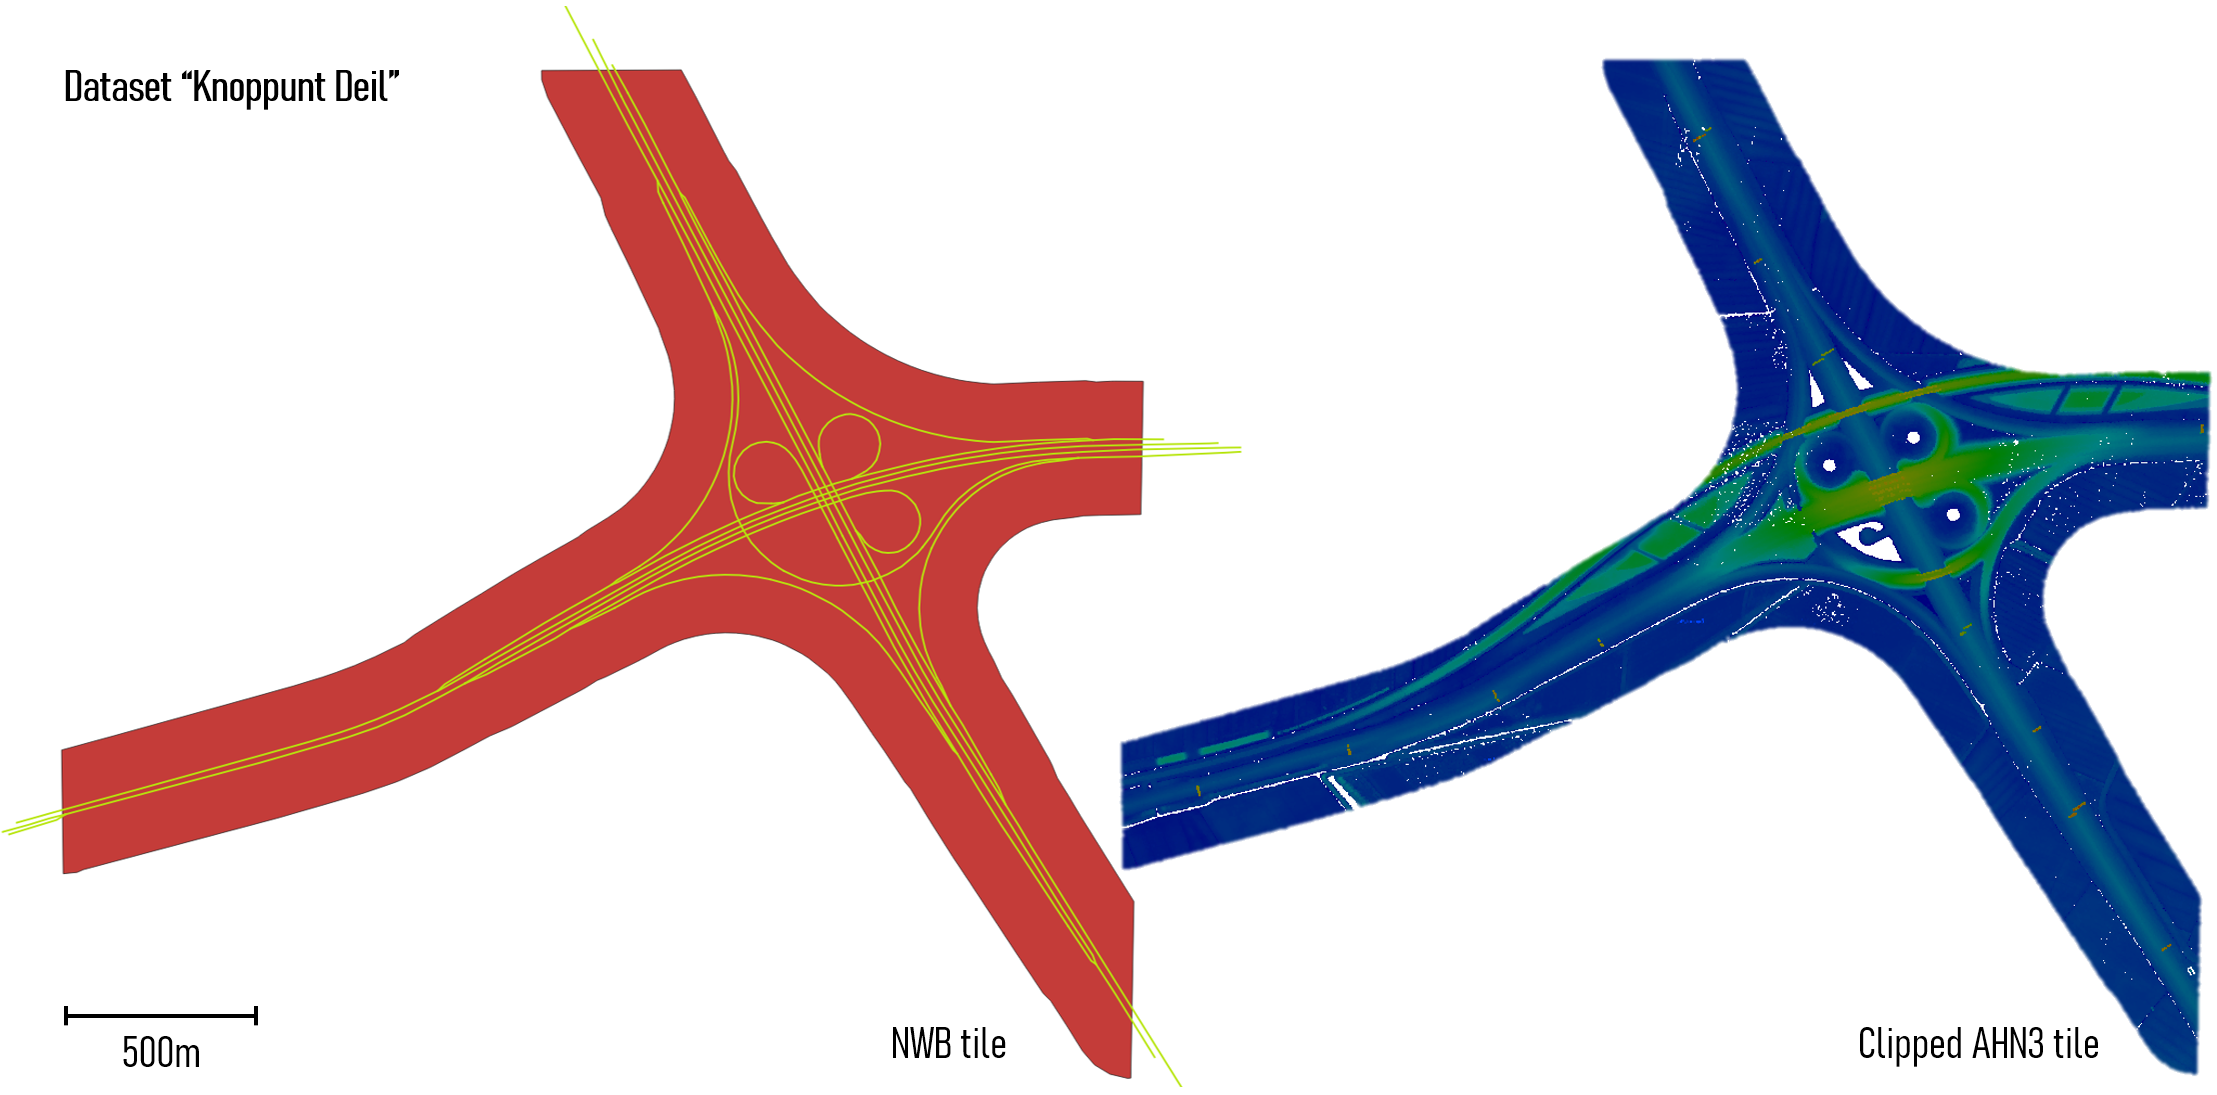
\includegraphics[width=\linewidth]{final_report/figs/manualpreprocessing.png}
    \caption[Visualisations illustrating the results of manual pre-processing]{Visualisations illustrating the results of manual pre-processing. An \ac{nwb} tile (yellow lines) and the corresponding Lidar clipping polygon (in red) are shown alongside the clipped point cloud tile (on the right). Darker areas represent lower elevations, the total elevation range shown is about 10 m.}
    \label{fig:manualpreprocessing}
\end{figure}

Implementing a scaling solution was not part of this project, although all parts of the implementation were designed in a way that a scaling framework could be added to it with a relatively small amount of effort. Among other things, scaling in this project concerns the need to subdivide the input data in a way that the software never runs out of memory while processing it. These subdivisions could be generated, in the simplest case, based on tiling, i.e. overlaying a 2D raster on the extents of the input datasets and cropping them to the extents of individual cells.

As scaling was not part of this project, the task of creating manageable subsets of the input data was carried out manually. The procedure consisted of cropping the input vector datasets (\ac{nwb}, \ac{dtb}) into tiles showing interesting and representative road layouts, and for each of them, creating an \ac{ahn3} file with those points, which are a set maximum distance from any relevant roads (\ac{r_roads} and \ac{p_roads}) in their respective \ac{nwb} tiles. For vector data processing, I used \textit{QGIS}, and for Lidar processing I used \textit{LASTools}.

I derived the area of interest in which to keep Lidar points by buffering the relevant centrelines in the \ac{nwb} tiles by 150 metres, and passing these geometries on to LASTools to use to \textit{clip} the relevant \ac{ahn3} tiles. \ac{ahn3} itself comes tiled in the official release (on a much larger scale), and I derived each testing dataset from a single \ac{ahn3} tile to keep the manual procedure simple. I also discarded \ac{ahn3} points not classed as ground or bridge points at this stage (2 and 26 respectively), as they are not relevant to our methods.

The relevant visualisations are shown in Figure \ref{fig:manualpreprocessing}. The clipping polygon was manually edited to have sharp, linear boundaries and \ac{nwb} \textit{wegvakken} intersecting its interior were included in the testing dataset. The resulting occasional overshoots of \ac{nwb} centrelines (relative to \ac{ahn3}) allowed me to test how well the procedure performs in areas where \ac{ahn3} is completely unavailable for a short distance, but where \ac{dtb} coverage is present. At the end of the research, they also turned out to cause unforeseen issues with accuracy assessment, which I discuss in Section \ref{sub:accuracytabulated}. On the right, the point cloud is shown in its original density, not a derived \ac{dtm}.

I created 11 testing datasets in total, each with its own cropped or clipped \ac{nwb}, \ac{dtb} and \ac{ahn3} files, which are described in the next section. The dataset shown in this figure is \textit{Knooppunt Deil} (from \ac{ahn3} tile \codeword{39CZ1}).

I picked 150 metres as a buffer distance for point cloud clipping not because I expected road surfaces to be so wide, but because I found that it reduced the volume of points to manageable levels in my testing tiles, while retaining plenty of neighbourhood information which I found to be useful for debugging purposes, and for the assessment of how well my algorithms perform in various environments next to roads - in other words, they provided context for the interpretation of intermediate results, and for the algorithms themselves. Using a smaller buffer distance would lead to slightly reduced runtimes.

\subsection{Description of testing datasets}
\label{sub:testingdata}

The set of chosen areas needed to be representative of the whole country to provide an insight into the effectiveness and performance of the algorithm in as many scenarios as possible. Furthermore, I also deliberately included areas which I thought would prove especially challenging, such as roads with many stationary vehicles, roads in multi-level 3D relationships (in motorway junctions), as well as tunnels.

Table \ref{tab:inventory} provides an inventory of these datasets. The tile identifier in the first column refers to those used in \cite{ahn3_download}; each dataset is found within a single \ac{ahn3} tile as I mentioned in the last section. The resulting datasets fit into memory easily even on a mediocre computer, and are also small enough to allow intermediate results to be visualised and interpreted quickly.

\clearpage

\begin{longtable}[c]{@{}p{2.8cm}p{6.8cm}c@{}}
\toprule
Title, tile  & Features & Render \\ \midrule
Markerwarddijk, \codeword{20BN1} & provincial road on a dike in the Markermeer. Very limited amount of terrain around the road. Road consistently build on ground, there are no bridge structures. & \raisebox{-0.94\totalheight}{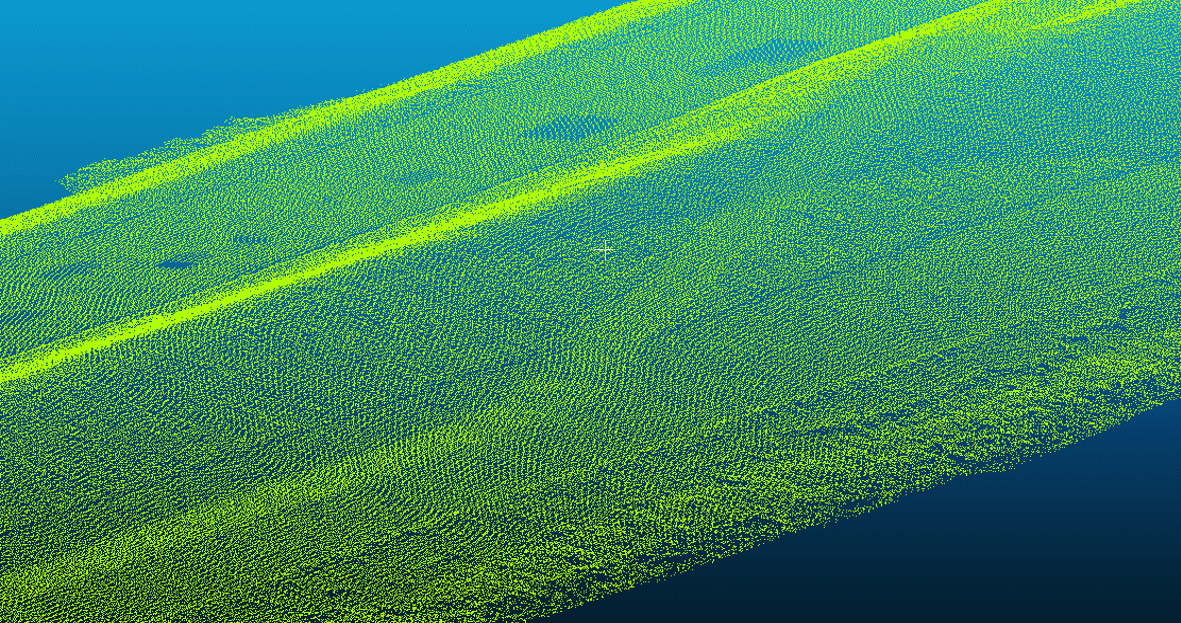
\includegraphics[width=6cm, height=3.5cm]{final_report/figs/ahn_sample_20BN1_a.png}}  \\
Amsterdam Hemhavens, \codeword{25BZ2} & Ringweg-West motorway as it crosses the IJ through the Coentunnel in a densely built-up environment. It is built on artificially elevated ground and on bridges in this area. Part of Westradweg also included, built entirely on a long bridge. & \raisebox{-0.94\totalheight}{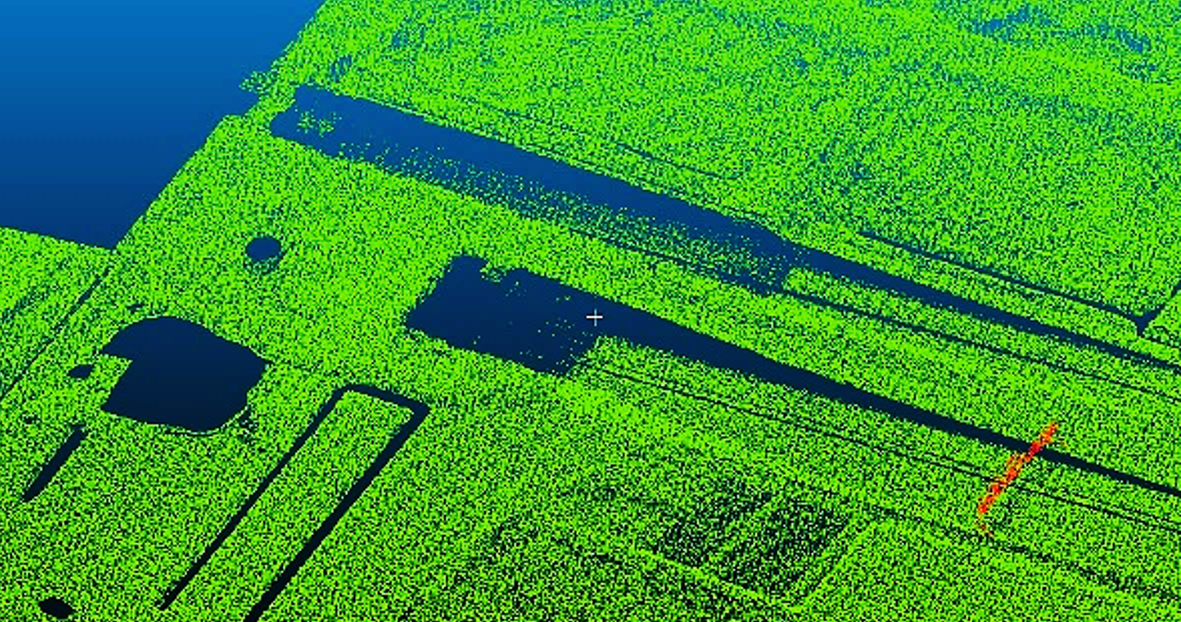
\includegraphics[width=6cm, height=3.5cm]{final_report/figs/ahn_sample_25BZ2_a.png}} \\
Amsterdam Zuid, \codeword{25DN2} & \ac{r_roads} with many closely spaced bridges, small tunnels, dense grouping of holes around roads due to presence of water and buildings & \raisebox{-0.94\totalheight}{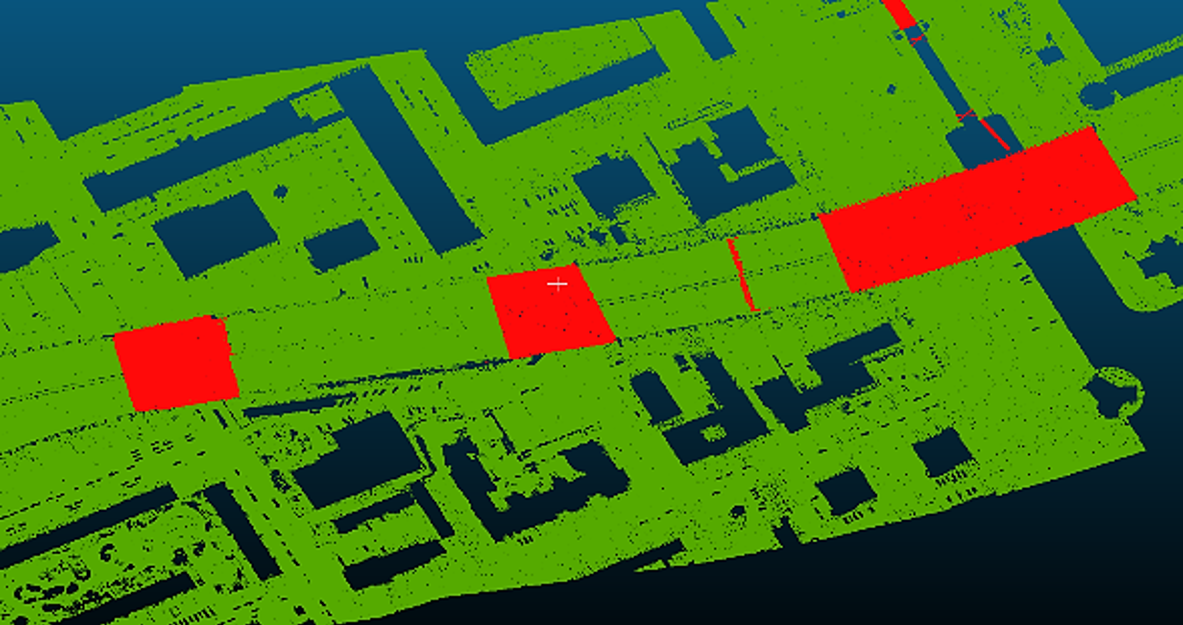
\includegraphics[width=6cm, height=3.5cm]{final_report/figs/ahn_sample_25DN2_a.png}} \\
Bunschoten, \codeword{32BN1} & \ac{p_roads} with three big roundabouts, and one road that ends in a small roundabout. Amersfoortseweg has its two lanes on separate road surfaces (like motorways), but with frequent connecting segments. & \raisebox{-0.94\totalheight}{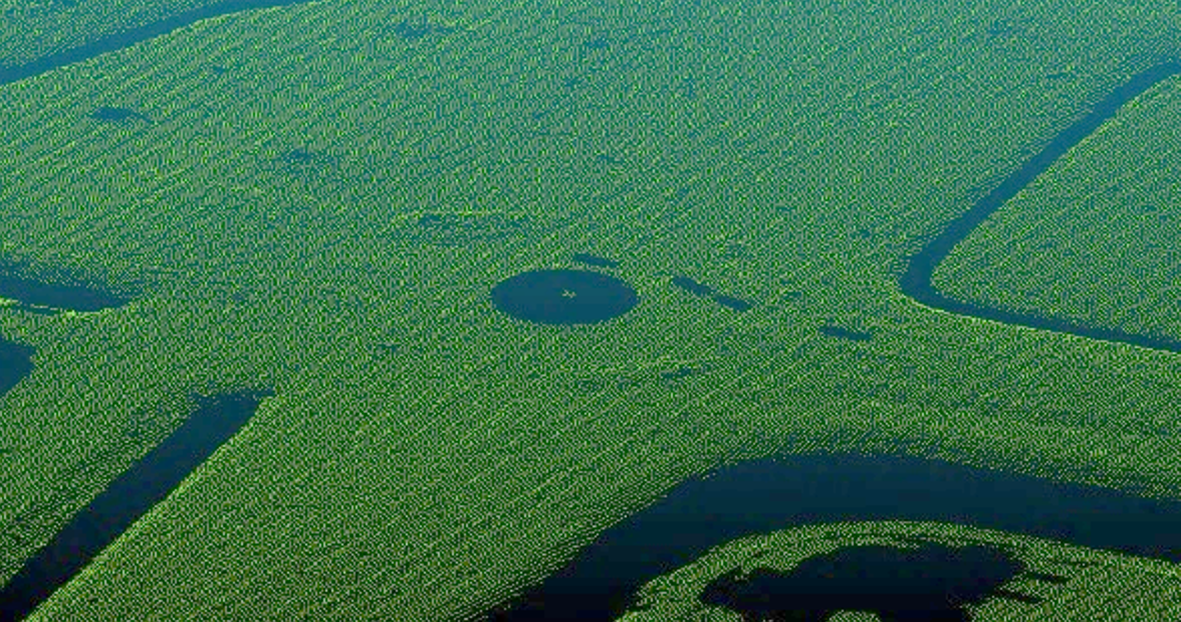
\includegraphics[width=6cm, height=3.5cm]{final_report/figs/ahn_sample_32BN1_a.png}} \\
Veluwe, \codeword{32FZ2} & Straight \ac{r_roads} surrounded by dense forest and crossed by wide wildlife overpasses. & \raisebox{-0.94\totalheight}{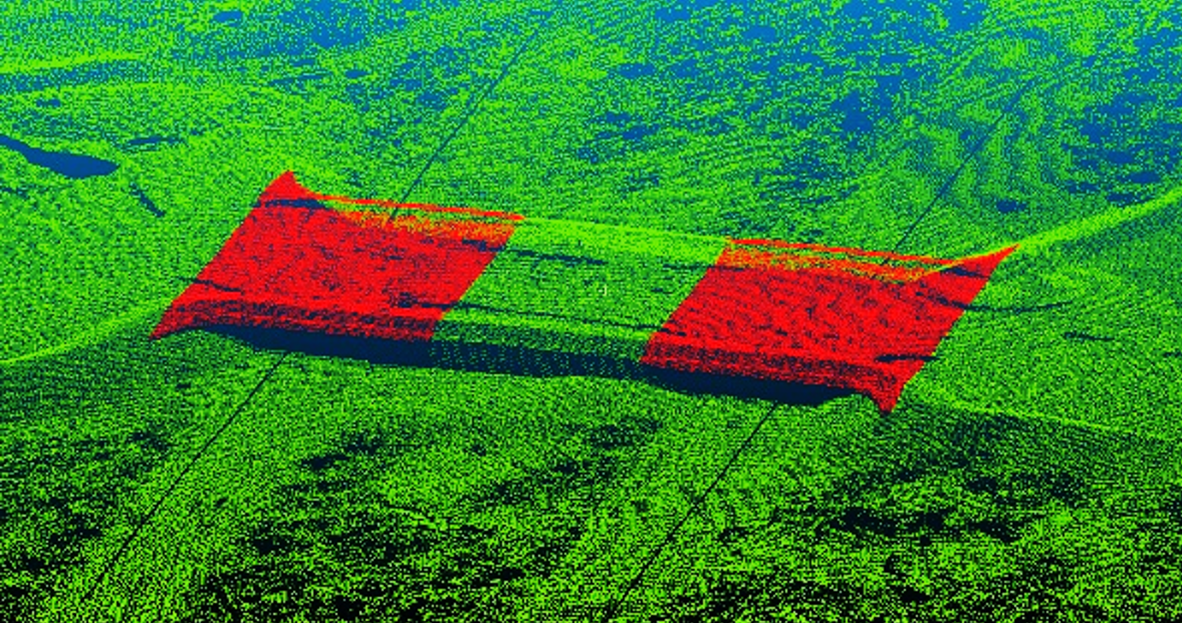
\includegraphics[width=6cm, height=3.5cm]{final_report/figs/ahn_sample_32FZ2_a.png}} \\
Apeldoornseweg, \codeword{32HZ2} & \ac{p_roads} in dense forest with canopy frequently occluding the road surface, decreasing point density and occasionally creating gaps. The road has small parallel branches running very close to it, which may make it difficult for the algorithm to distinguish between them. It also has roundabouts. & \raisebox{-0.94\totalheight}{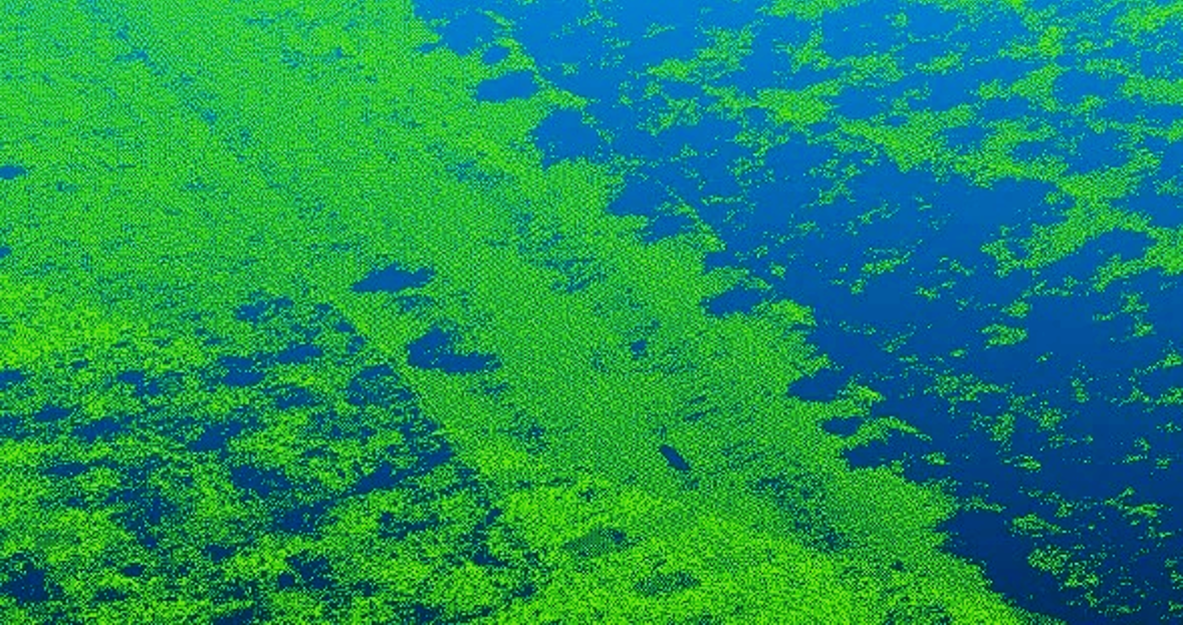
\includegraphics[width=6cm, height=3.5cm]{final_report/figs/ahn_sample_32HZ2_a.png}} \\
Hoenderloo, \codeword{33CN2} & \ac{p_roads} in extremely dense, continuous forest with canopy frequently occluding the road surface, decreasing point density and occasionally creating gaps. Both lanes are on the same road surface & \raisebox{-0.94\totalheight}{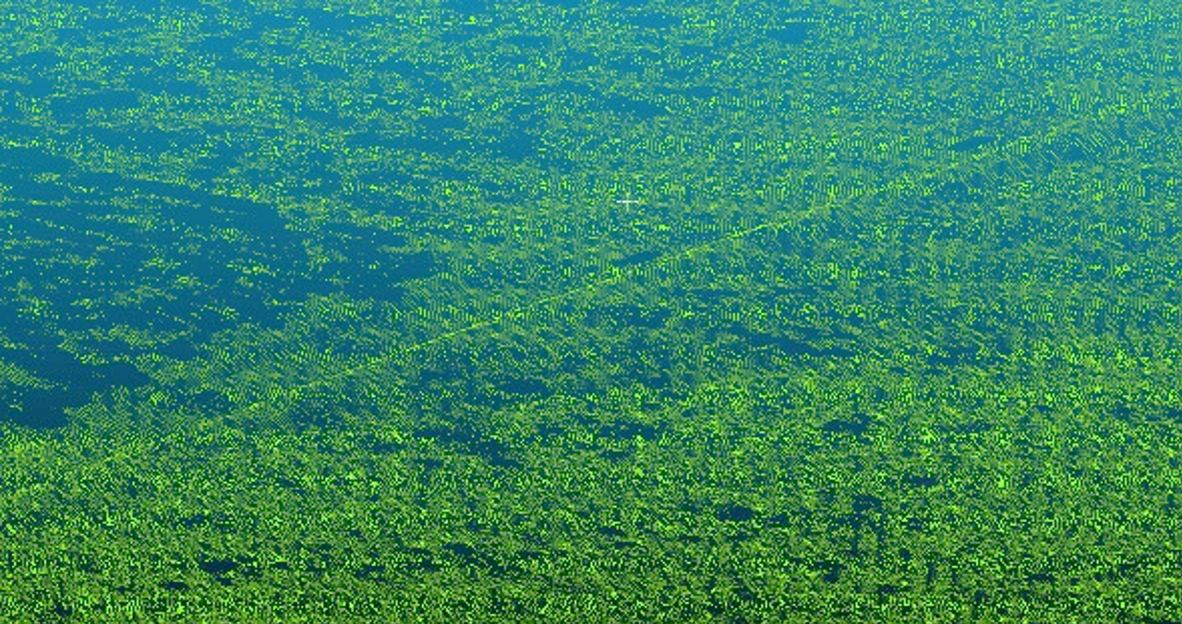
\includegraphics[width=6cm, height=3.5cm]{final_report/figs/ahn_sample_33CN2_a.png}} \\
Rotterdam Ketheltunnel, \codeword{37EZ1} & This segment of the A4 heading North from Rotterdam has been recently reconstructed in an underground tunnel. In addition, a significant portion of this motorway now runs in a trench towards Delft. \ac{ahn3} was imaged during the reconstruction, and hence contains anomalous data about the road surface. & \raisebox{-0.94\totalheight}{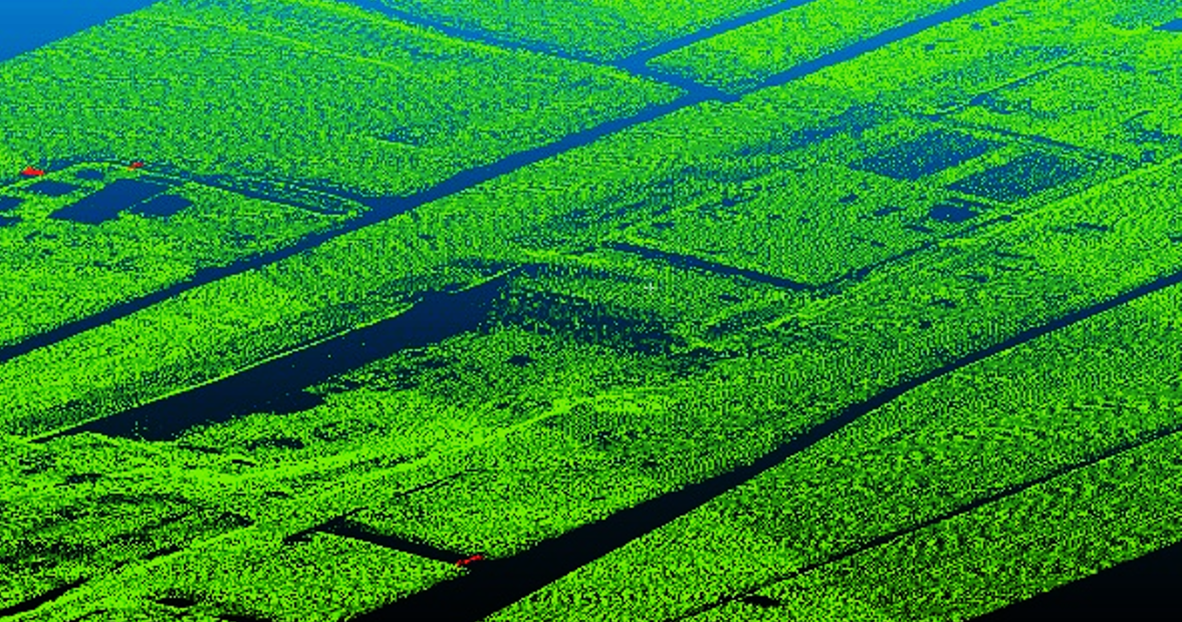
\includegraphics[width=6cm, height=3.5cm]{final_report/figs/ahn_sample_37EZ1_a.png}} \\
Knooppunt Ridderkerk, \codeword{37HN2} & The Ridderkerk junction is one of the largest of its kind in The Netherlands, in one place containing 4 overlapping \ac{r_roads}. Furthermore, it contains a high density of \ac{r_roads} in a small area, many of them very tightly packed. Many of them have very sharp bends. & \raisebox{-0.94\totalheight}{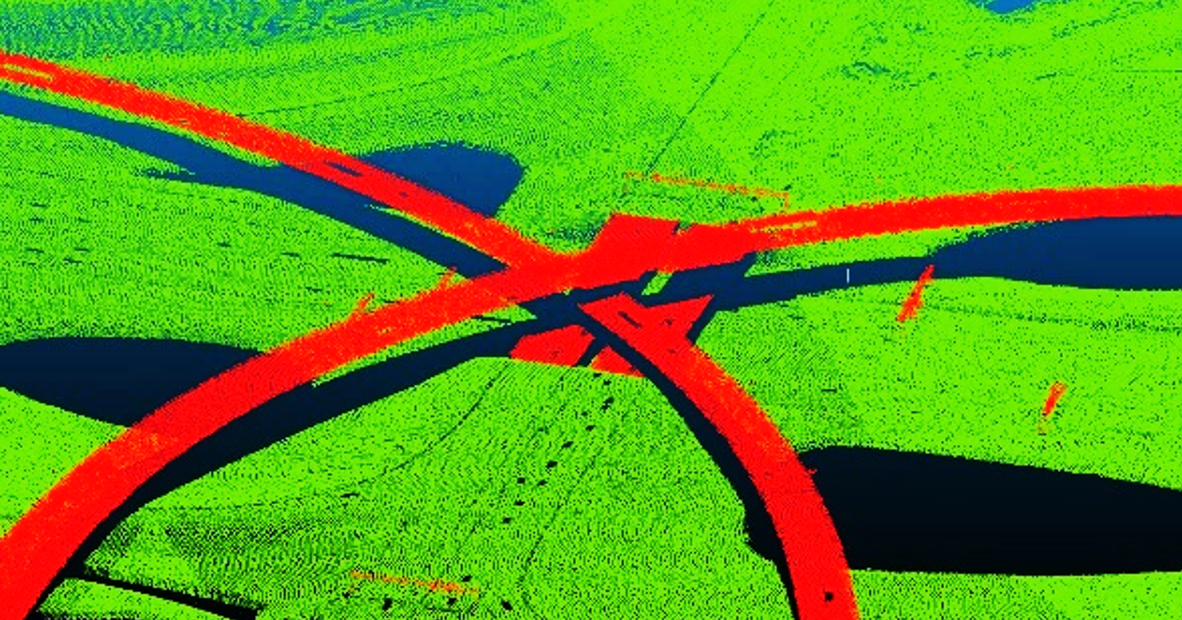
\includegraphics[width=6cm, height=3.5cm]{final_report/figs/ahn_sample_37HN2_a.png}} \\
Gorinchem, \codeword{38GZ1} & Complex junction between \ac{p_roads} and \ac{r_roads} with small ramps, roundabouts and overlapping geometries. & \raisebox{-0.95\totalheight}{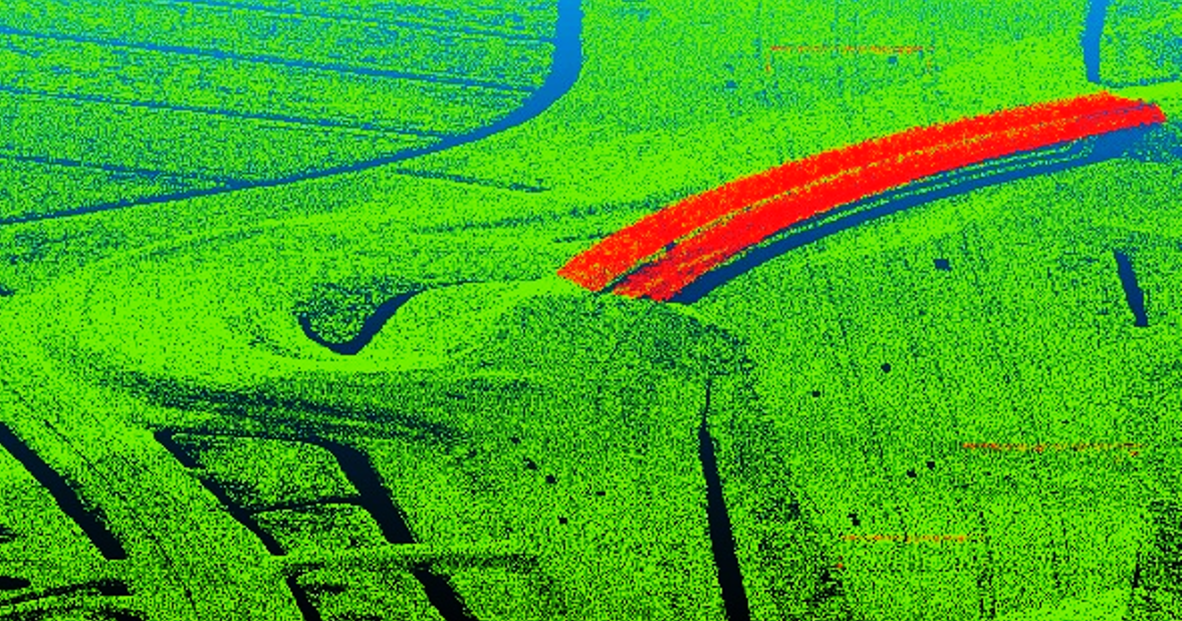
\includegraphics[width=6cm, height=3.5cm]{final_report/figs/ahn_sample_38GZ1_a.png}} \\
Knooppunt Deil, \codeword{39CZ1} & Less complex, but analogous junction to the Knooppunt Ridderkerk. & \raisebox{-0.5\totalheight}{\textit{Please refer to Figures \ref{fig:ahnbridges}, \ref{fig:ahnsigns}, \ref{fig:ahnnwb} and \ref{fig:dtbahn}.}} \\
\toprule
\caption[Inventory of the testing datasets]{Inventory of testing datasets. In the renders, ground points are shown in green and bridge points in red.}
\label{tab:inventory}
\end{longtable}

One instance of my software can process a single testing dataset at a time. However, running multiple Python instances in parallel allows one to easily parallel-process multiple tiles depending on the CPU installed in the computer. Each dataset consists of a cropped \ac{nwb} and \ac{dtb} file, and the clipped \ac{ahn3} point cloud.

All datasets mentioned in Table \ref{tab:inventory} are part of the GitHub release of the results. A compressed archive with the input testing files (as well as all intermediate results and the final results) can be downloaded via a link found in the repository's readme file.

\section{Results of processing steps}
\label{sec:results}

The results below are presented in the same section structure as the detailed methods were in Section \ref{sec:methods} of the previous chapter. This is intended to make it easy for readers to correlate the results with the theory underlying the relevant processing mechanisms. In each section, I describe - with the help of 3D visualisations - how well each processing step performs, and how effective and useful they are in the context of the entire pipeline as a whole. I also devote attention to describing typical scenarios in which algorithms are useful and perform well, as well as ones where the opposite is true and they may produce sub-optimal results. Since the section structure also corresponds to the overall implemented pipeline structure, in each of the pipeline steps I describe how exactly the underlying software implementation is meant to be used, with notes on the recommended arguments.

\subsection{Splitting NWB into NBRS}
\label{sub:r_nbrsgeneration}

Each colour in Figure \ref{fig:nbrsgeneration0} corresponds to a specific \ac{nbrs} ID, meaning that LineStrings (\textit{wegvakken}) belonging to the same \ac{nbrs} are coloured the same. The figure demonstrates that as a result of the \ac{nbrs} generation step, the cropped road network becomes semantically enriched with identifiers linking certain LineStrings together, based on semantic or geometric conditions depending on which algorithm was used.

The colours are generally inconsistent between the results of the two algorithms (top and bottom parts of the figure). The same colour scheme was used to generate the two figures, but the two algorithms distribute \ac{nbrs} IDs differently.

\begin{figure}
    \centering
    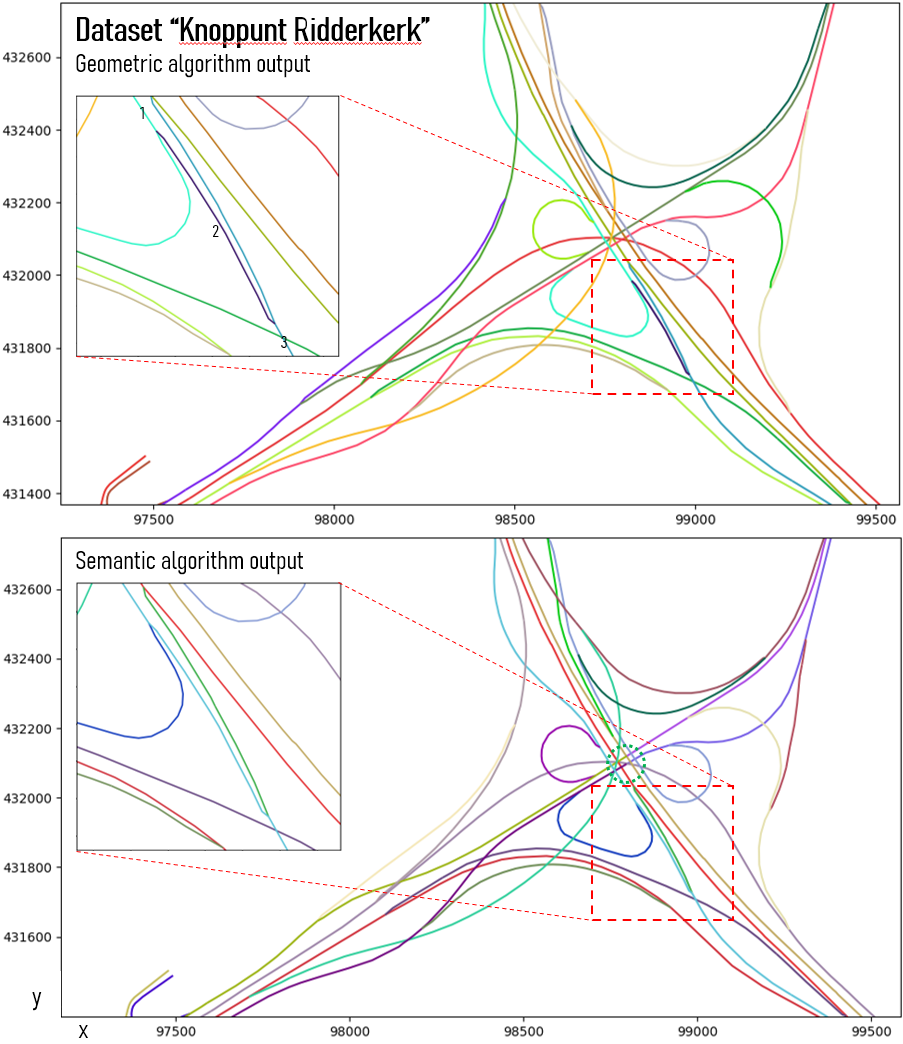
\includegraphics[width=\linewidth]{final_report/figs/nbrsgeneration0.png}
    \caption[Renders illustrating the results of NBRS generation]{Visualisations illustrating the results of \ac{nbrs} generation. The colour-coding was randomly generated based on the generated ID numbers of the NBRS. The insets and annotations highlight differences between the results of the two algorithms, which are further explained in the text.}
    \label{fig:nbrsgeneration0}
\end{figure}

\subsubsection{Issues with geometric algorithm}

Figure \ref{fig:nbrsgeneration0} also serves to illustrate the fundamental differences that exist between the results of the two algorithms. The geometric algorithm makes the assumption that the 2D georeferencing of \ac{nwb} is fully representative of the real-life geometry of road centrelines. However, I found this to be violated in various places as already mentioned in Section \ref{sub:nwb}. In short, where \ac{r_roads} intersect (this includes ramps, motorways and all combinations thereof), they often do so at abrupt angles, which can be observed in various places in Figure \ref{fig:nbrsgeneration0}, and especially in the insets. These angles are not representative of the real-life road geometry, they were drawn manually by data handlers to ensure that \ac{nwb} complies with certain external requirements. Consequently, they may prevent correct decisions from being made based on the intersection angles.

In places where this problem exists, choosing the straightest continuation across an intersection when building an \ac{nbrs} does not necessarily represent the optimal choice, because the angles are artificial. This can be observed in the inset of the top chart in Figure \ref{fig:nbrsgeneration0}, where I numbered some of the \ac{nbrs} on the geometric results. While the geometric algorithm obviously made the right choice \textit{based on the angles} between the individual road segments concerned, \textit{attribute table data} told the semantic algorithm that the role and road number of certain parts of \ac{nbrs} 0 and 2 are the same as that of \ac{nbrs} 1, which resulted in these parts of \ac{nbrs} 0 and 2 connecting via \ac{nbrs} 1. The "discarded" ends of \ac{nbrs} 0 and 2 then became two unique \ac{nbrs} by themselves. In the large-scale context of the road network, the semantic algorithm evidently made the correct choice, even though this introduced some small, abrupt internal angles into the \ac{nbrs}.

\subsubsection{Issues with semantic algorithm}

The green dotted circle in the semantic \ac{nbrs} generation results points out a place where the role and road number of a ramp changes suddenly, outside of a real-life intersection, which results in the algorithm abruptly starting a new \ac{nbrs} there. This is indicated by a change of colour from dark to light purple. The break happens in an unfortunate location, in the middle of a multi-level junction where the continuation of \ac{nbrs} is crucial so that large-scale trends across the complicated zone may be recognised effectively in later steps. This demonstrates that while the geometric algorithm is sensitive to problems with the georeferencing of the data, the semantic algorithm is sensitive to issues with the attribute table data. Within the testing tiles I examined, the two algorithms offered a comparable amount of benefits and drawbacks.

\subsubsection{Evaluation and choice of algorithm}

Both algorithms produce usable results overall. In general, the resulting chains of LineStrings satisfy all the original requirements I set for the outputs of this step (minimise internal angles, maximise length, disallow self-intersections and branching). Based on some further testing after implementing the rest of the pipeline, I also verified that the choice of algorithm does not significantly influence the output of subsequent steps.

Since the geometric algorithm generalises to arbitrary road networks better than the semantic algorithm (i.e. does not rely on specific properties of \ac{nwb}), I used it to generate the rest of the results shown and discussed in this report.

\subsubsection{Using the implementation}

In the software, before \ac{nbrs} generation can be executed, the \codeword{nbrs_manager} class needs to be initialised with the file path to the cropped \ac{nwb} file of the desired dataset. Example calls to perform geometric \ac{nbrs} generation are provided below.

\begin{verbatim}
roads = nbrs_manager(fpath = nwb_fpath)
roads.generate_nbrs(algorithm = 'geometric')
\end{verbatim}

In the code snippet above, \codeword{nwb_fpath} refers to a variable containing the file path to the cropped \ac{nwb} file of the desired testing dataset. For instance, the file path could end in \codeword{.../C_39CZ1_nwb.shp}, using the naming convention of the released testing files, the dataset called \textit{Knooppunt Deil} is desired. Switching to \codeword{algorithm = 'semantic'} triggers the use of the semantic algorithm.

The invocation \codeword{roads.plot_all()} may be executed to plot the results on a 2D diagram using random colours to distinguish between \ac{nbrs}. At this point, \ac{nbrs} generation results are saved in class variables only (see \codeword{roads.nbrs_wvkn}), hence running \codeword{roads.write_all()} at this point is \textbf{not} going to write the \ac{nbrs} IDs into the attribute table. The imported road network is stored in \codeword{roads.nwb} in a GeoDataFrame which also contains the generated \ac{nbrs} IDs.

\subsection{Elevation estimation}
\label{sub:r_elevationestimation}

\begin{figure}
    \centering
    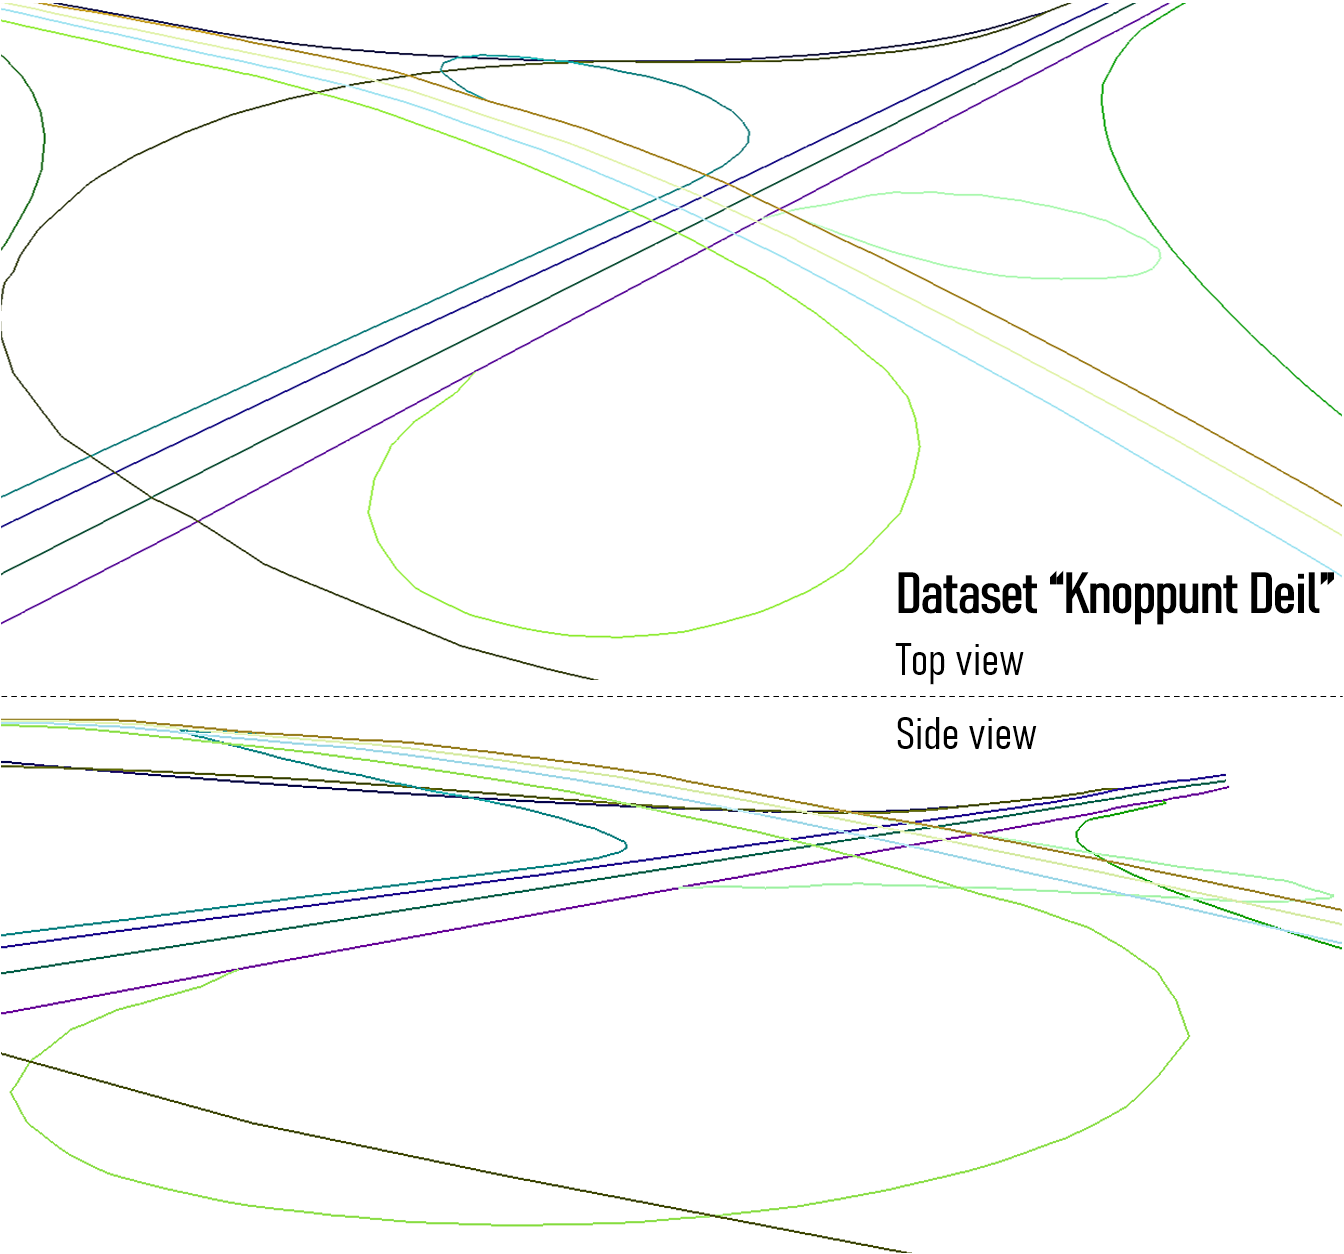
\includegraphics[width=\linewidth]{final_report/figs/elevationestimation0.png}
    \caption[Visualisations illustrating the preliminary elevation estimation results]{Visualisations illustrating the preliminary elevation estimation results. The colour-coding of the 3D NBRS lines was randomly generated based on their \ac{nbrs} IDs.}
    \label{fig:elevationestimation0}
\end{figure}

Figure \ref{fig:elevationestimation0} shows the results of this step in two 3D visualisations. The \ac{nwb} centrelines are now shown at their estimated elevations. The figure contains two visualisations that allow the reader to examine the same results from multiple viewing angles. 

\textit{The vertical dimension in this visualisation and all other 3D visualisations in this chapter are exaggerated 5-fold, so that changes in elevation are made better visible.}

\subsubsection{Vertex densification}

\begin{figure}
    \centering
    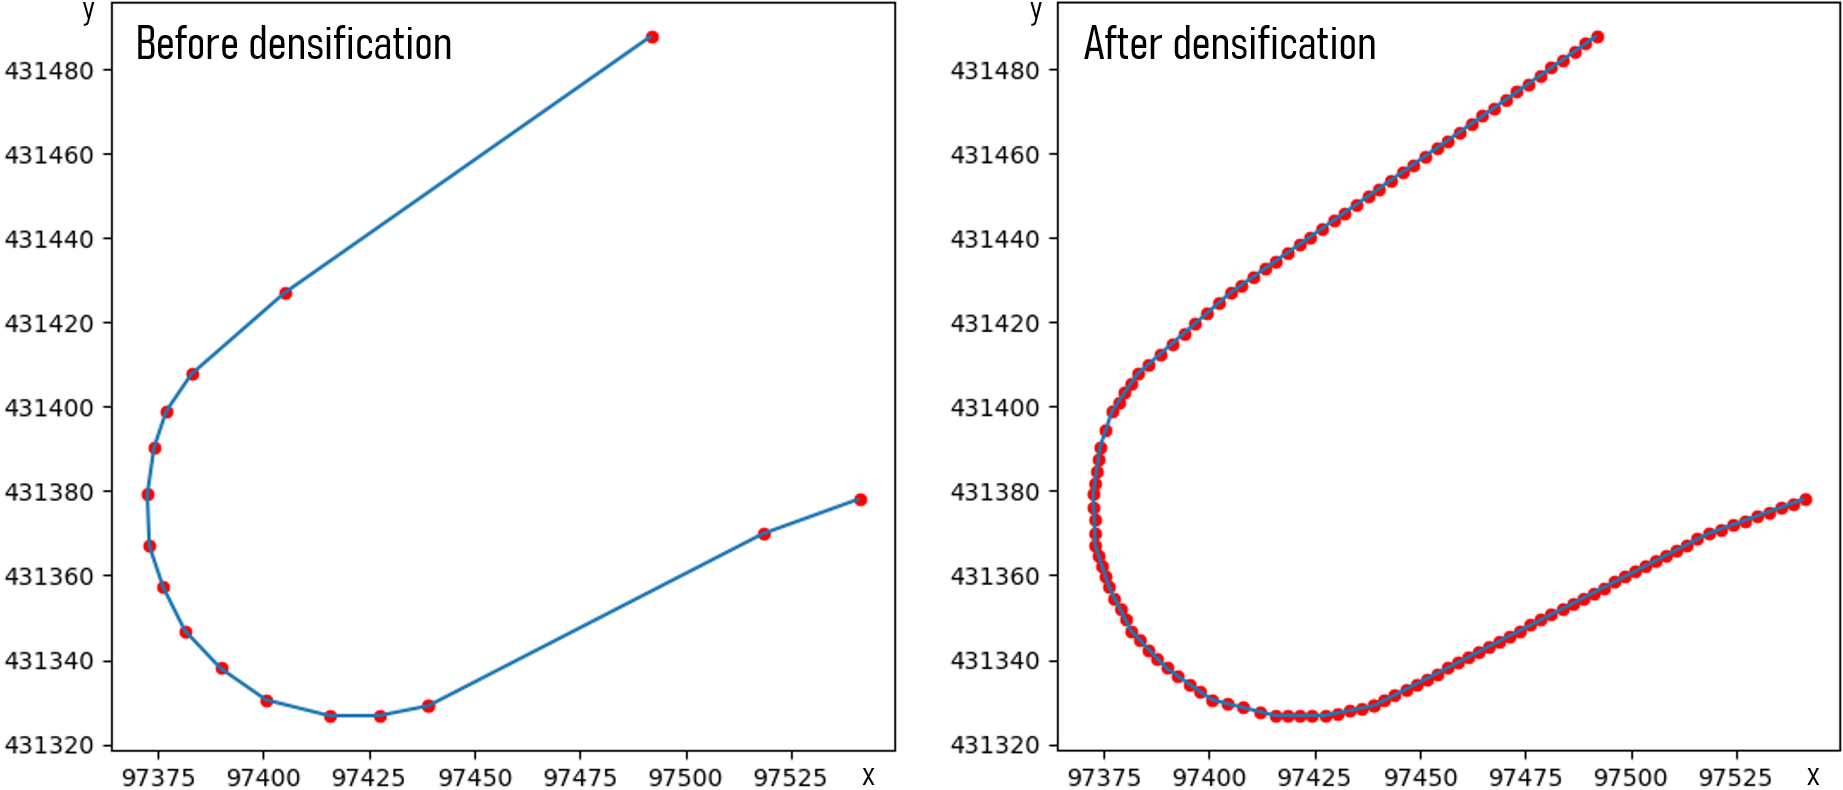
\includegraphics[width=\linewidth]{final_report/figs/elevationestimation1.png}
    \caption[Visualisations illustrating vertex densification]{Plots illustrating vertex densification. Vertices are marked as red circles on the blue \ac{nbrs}.}
    \label{fig:elevationestimation1}
\end{figure}

The vertices were densified before running preliminary elevation estimation; I used a threshold of 5 metres for all my final results. This means that no individual line segment in the 3D road network is longer than 5 metres. I found this threshold value to offer a compromise between longer processing times (in later steps) and more refined results.

We may say that while the horizontal dimensions were merely oversampled, the vertical sampling benefited from the vertex densification in the sense that it is far more detailed than it would be without it (as also mentioned in Section \ref{sub:m_elevationestimation}). An example visualisation of what happens to a specific \ac{nbrs} during vertex densification is shown in Figure \ref{fig:elevationestimation1}.

\subsubsection{Types of challenging scenarios}

Instead of focusing on details, I will only comment on the general quality of the results, since accuracy is not yet important at this step - this 3D conversion is merely a stepping stone towards the goal of performing Lidar segmentation. It only needs to help find candidate points for the subclouds, rather than to be a perfect representation of 3D road geometry. In fact, in practice it just needs to be closer to the relevant road surface, than to other roads (or other occluding objects) above or below it.

The are two main aspects of the output that require our attention: how well the 3D centrelines conform with the real-life road surfaces (effectiveness of the 3D conversion), and how succesfully outliers are being eliminated (effectiveness of the refinement step). The former can be assessed via a visual comparison with the underlying \ac{ahn3} point clouds, while the latter can be examined by looking for artefacts at locations where occlusion happens. Figure \ref{fig:elevationestimation2} shows two further 3D visualisations that contain examples of the features that are relevant for this assessment.

\subsubsection{Effectiveness of 3D conversion}

The top visualisation in Figure \ref{fig:elevationestimation2} illustrates that in the case of flat lengths of roads, centrelines are generally positioned very close to the Lidar-defined road surfaces (within a few centimetres in general). Outliers are atypical in well-exposed areas, corresponding to the lack of outliers in \ac{ahn3} itself (and its ground classification). The procedure is fast, runtimes for the testing datasets are generally in the range of 1 to 5 seconds on a mediocre computer.

\begin{figure}
    \centering
    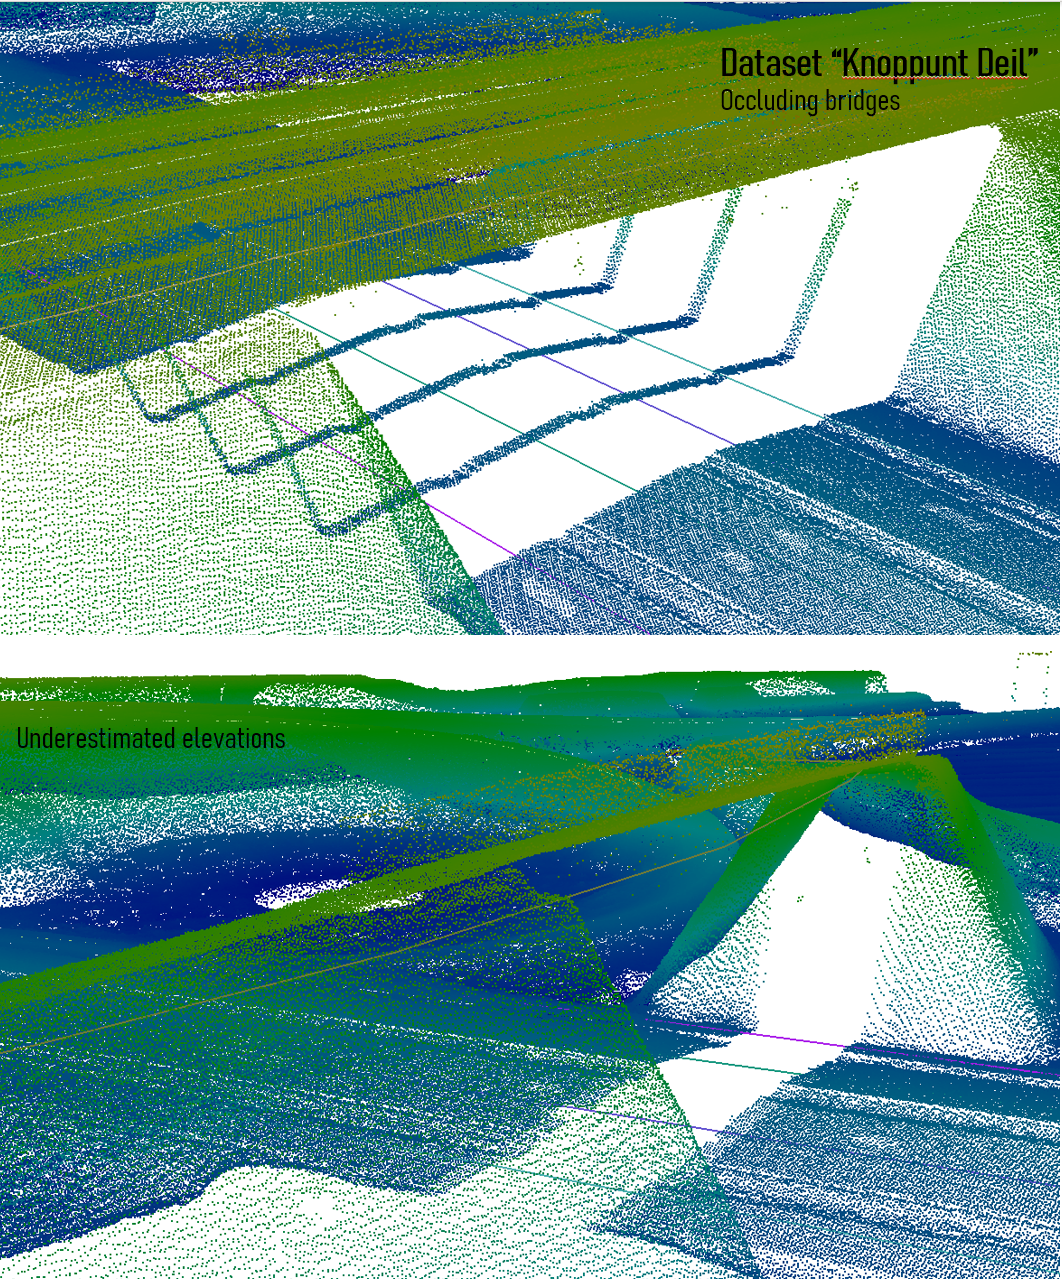
\includegraphics[width=\linewidth]{final_report/figs/elevationestimation2.png}
    \caption[Visualisations comparing the preliminary 3D-NWB with AHN3]{Visualisations comparing preliminary 3D conversion results with the \ac{ahn3} point cloud. The colour-coding of the 3D \ac{nbrs} lines was randomly generated based on their ID numbers. Darker areas represent lower elevations, the total elevation range shown is about ten metres.}
    \label{fig:elevationestimation2}
\end{figure}

Thinning the input point cloud aggressively can marginally improve the performance of this step, but it also drastically reduces its effectiveness in areas that are poorly sampled. This in turn may result in artefacts on a scale that may also confuse the refinement step. I found that working with no thinning applied, or a maximum thinning factor of 3 (33\% of points kept) at most, works best. My final configuration uses a thinning factor of 2 when it imports the \ac{ahn3} data, which is carried over to all subsequent steps that work with it.

There is a range of factors that may result in the computation of anomalous preliminary elevations due to occlusion. Firstly, if an \ac{nwb} centreline is positioned far from the actual road centreline (or next to the road), then the 3D elevations will be derived from a patch of Lidar points that may include a significant number of off-road points. This may result in both positive and negative outlier elevations being computed relative to where \ac{nwb}'s georeferencing is correct. Furthermore, bridges in \ac{ahn3} include reflections from civil engineering structures, which are often attached to roads close to their edges. If the centreline of an \ac{nbrs} falls too close to the edge of the road where such objects are present, its elevations may be corrupted by Lidar points reflected from them, rather than from the road surface.

Furthermore, slow or stationary vehicles and motorway signs (due to their presence in classification 26), and larger occluding objects (e.g. bridges built \textit{over} a given road) tend to generate a sequence of outlier vertices, depending on the size of the object. Gaps in \ac{ahn3} coverage (e.g. where a road passes underneath water in a tunnel) can also give rise to missing elevations in the output of this step. Both the outlier elevations and the missing elevations resulting from these artefacts are mostly eliminated by the refinement step.

The query radius used in the KD-tree queries in my final configuration is 1 m. At the typical local posting distances found in \ac{ahn3}, this represents a compromise between fetching enough samples to minimise the effects of small-scale outliers and minimising the chances of including off road points where \ac{nwb} deviates from its optimal position. This query radius corresponds to a query area of $\pi$ m\textsuperscript{2}, which typically corresponds to selecting about 30 to 120 \ac{ahn3} points in practice, depending on the local sampling density (assuming a thinning factor of 2 was used).

\subsubsection{Effectiveness of refinement step}

The effects of the refinement step can be observed in the shape of the \textit{lower} set of 3D centrelines shown in the top visualisation in Figure \ref{fig:elevationestimation2}. The series of bridges causes occlusion, meaning that Lidar coverage is intermittent for the lower set of roads, for a distance of about 70 metres. Initially (before the refinement step), the centrelines of the lower set of motorway lanes thus became snapped to the elevation of overlying roads. The resulting outliers were easily identified using the polynomial model that was fitted on the \ac{nbrs}, and new values were interpolated linearly.

For my final results, I used a degree of 8 for the fixed-degree polynomials, and set the outlier filtering threshold to 0.2 times the standard deviation of the data-model errors in the given polynomial fit. I found that in general these parameters work best with the testing datasets. Standard deviations below 0.4 metres are artificially increased to 0.4 metres to avoid modifying elevations in roads whose conformance with the model was already found to be near-perfect.

This approach proved to be an effective solution in terms of eliminating occlusion-related artefacts. It is ineffective only in places where the occluding geometry is very close to the road surface. For instance, stationary vehicles occasionally introduce outliers that are not far enough from the model to be detected in the refinement step, thereby giving rise to small spikes in the output. This does not happen frequently, and does not represent a problem in the context of the pipeline as a whole. This step also replaces outliers caused by motorway signs.

The optimal lower limit for the outlier filtering threshold is determined, in practice, by the accuracy of the polynomial fits themselves. If the value is set too low, elevations that were in fact already correct may be replaced with values from poor polynomial fits. This issue arises where the vertical curvature of the modelled roads is unusually complex, such as in the overpass shown in the bottom visualisation in Figure \ref{fig:elevationestimation2}. Complex curvature is difficult to approximate using fixed-degree polynomials, which becomes especially relevant when processing very long \ac{nbrs}.

Even when using a sufficiently high outlier filtering threshold, the algorithm may occasionally identify lengths of such roads as outliers and reposition them to the incorrect elevation level suggested by the polynomial model. I successfully bridged this relatively uncommon issue by taking it into account while implementing the Lidar segmentation workflow. Therefore, these inaccurate elevations do not represent a problem on the scale of the pipeline as a whole, because the next pipeline step is not sensitive to them. Shorter \ac{nbrs} lengths could help deal with this problem in a more explicit manner, but this would also mean that certain longer trends would become impossible to model later on.

Using general curve fitting or an interconnected set of splines (in place of fixed-degree polynomials) could help solve this issue in a more direct manner, but the toll this would take on computational complexity and the complexity of the code is not justified by the issues that arise.

\subsubsection{Using the implementation}

The below code snippet shows the code that I used to generate my final results.

\begin{verbatim}
roads.densify(thres = 5)
roads.estimate_elevations(fpath = ahn_fpath, r = 1, thin = 2)
roads.write_all(fpath = simpleZ_fpath)
\end{verbatim}

The first line performs vertex densification with a threshold of 5 metres. The second line performs the preliminary elevation estimation (and refinement) step, the variable \codeword{ahn_fpath} is assumed to contain a file path to the clipped \ac{ahn3} file belonging to the desired testing dataset. For instance, it could be \codeword{.../C_39CZ1_2_26_clipped.las} using the naming convention of the input files I released on GitHub. The tags \codeword{_2_26_clipped} in these file names refer to having kept only points in classes 2 and 26 (ground and bridge points respectively), and having clipped it to the extents of buffered centrelines. The variables \codeword{r} and \codeword{thin} control the query radius and thinning factor respectively, their default values are shown.

The last line of code writes the resulting 3D geometry to disk, "mimicking" the structure of the input file. The variable is named in such a way to distinguish it from the variable containing the file path where the final 3D-NWB results will be written, called \codeword{accurateZ_fpath}. This step is optional, it is intended for debugging and demonstration purposes only.

In the class itself, the results of this step are not stored in a separate variable, but are added to the GeoDataFrame representation of the input \ac{nwb} Shapefile, found in the \codeword{.nwb} variable of the \codeword{nbrs_manager} class.

\subsection{Lidar segmentation}
\label{sub:r_lidarsegmentation}

\begin{figure}
    \centering
    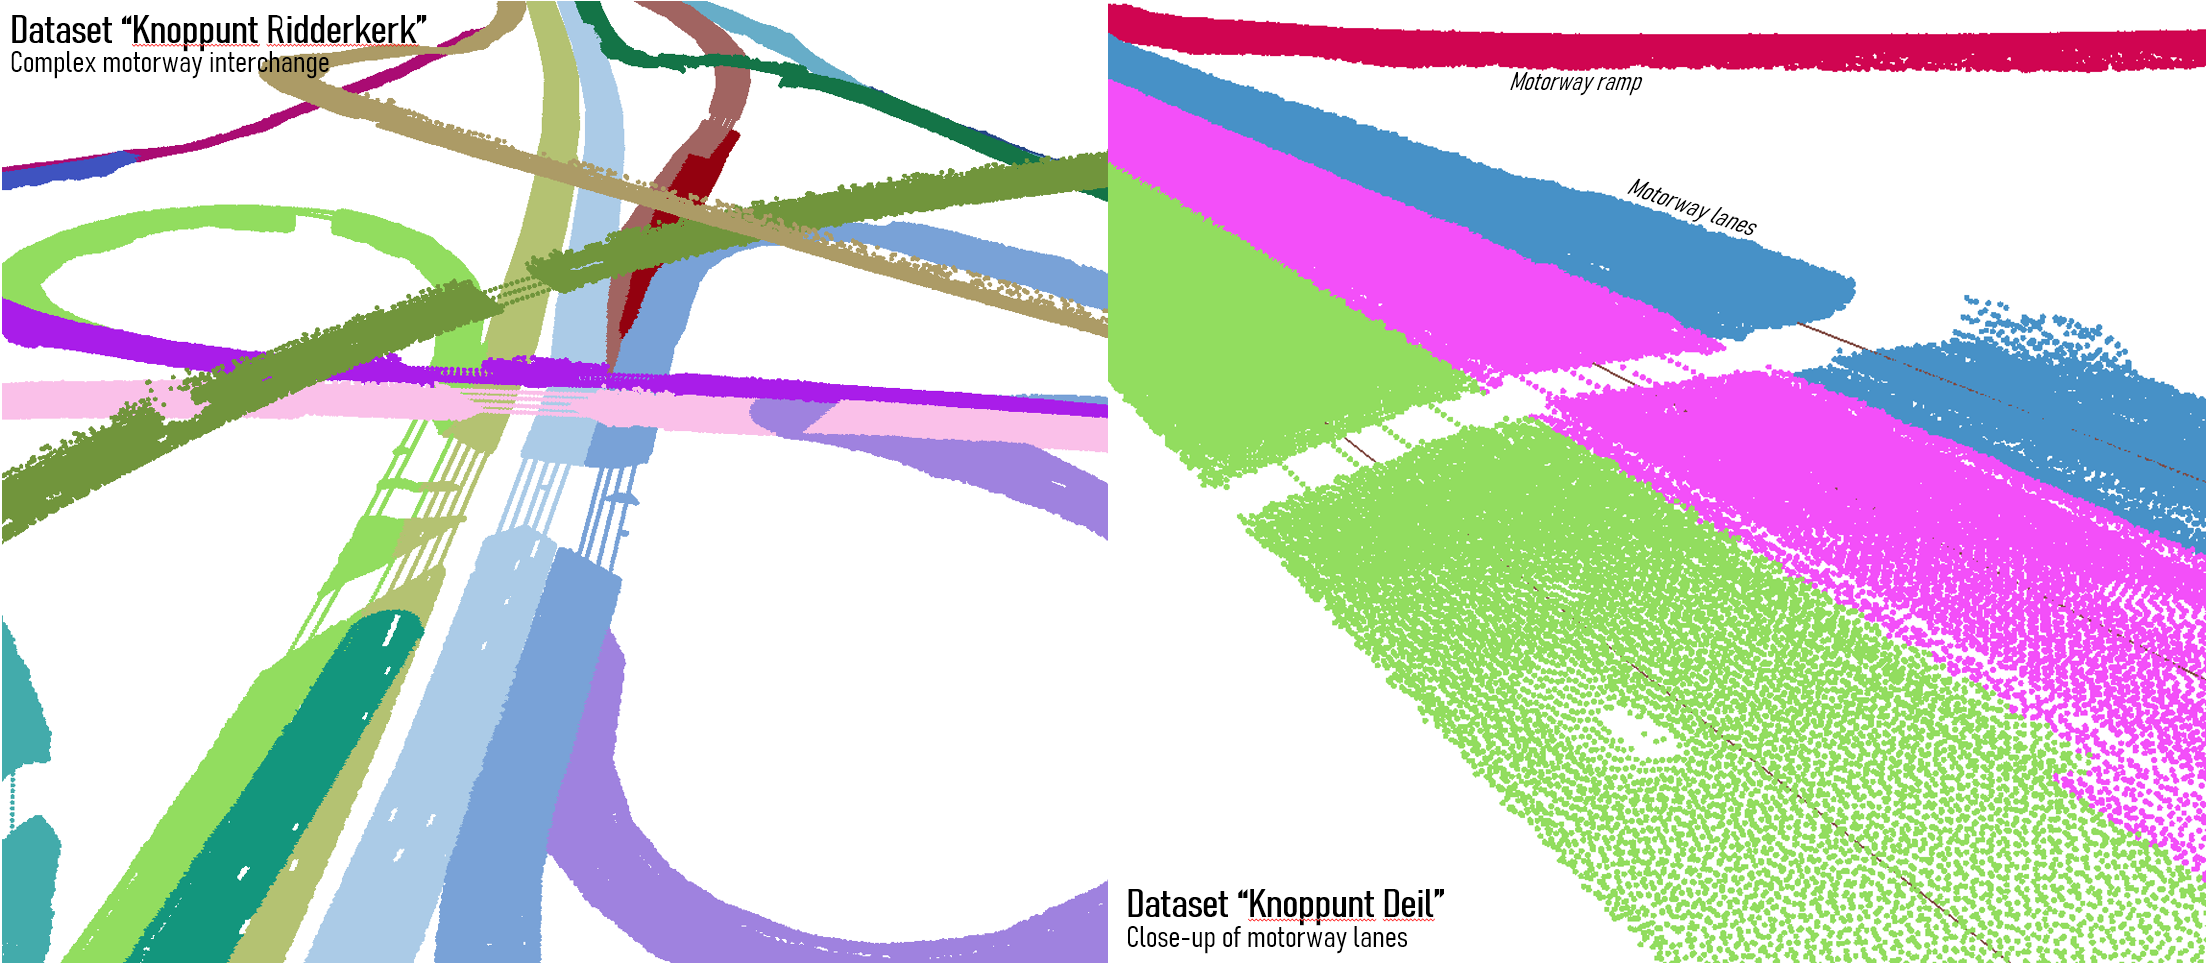
\includegraphics[width=0.86\linewidth]{final_report/figs/lidarsegmentation0.png}
    \caption[Visualisations illustrating the results of Lidar segmentation]{Visualisations illustrating the results of Lidar segmentation. The colour-coding of the subclouds was randomly generated based on their NBRS IDs. In the bottom part of the figure, the centrelines are also shown in black.}
    \label{fig:lidarsegmentation0}
\end{figure}

Figure \ref{fig:lidarsegmentation0} shows some visualisations of the results of Lidar segmentation. For subclouds which are positioned far from each other, a clear separation is observable. Ones that are close to one another often overlap, such as in various places in the top visualisation. This is the result of there not being much space between the roads themselves. The overlapping parts of such subclouds may contain duplicate points (in other words, points may be part of multiple subclouds). Out of these "duplicate" points, the visualisation only shows the ones that were loaded last, hence some subclouds may appear thinner than they are.

\subsubsection{General description of results}

The properties which we are looking for in the resulting subclouds is that they contain as many of the road surface points, and as few of the surrounding unrelated points, as possible - especially with regards to points reflected from occluding objects. Figure \ref{fig:lidarsegmentation0} illustrates quite vividly that indeed, each \ac{nbrs}'s subcloud is clearly related to the underlying real-life road surface and that very few unrelated points are included.

Since this is not yet the stage where conservative thresholds are enforced, it is possible that a small number of unrelated points will be retained. This mostly happens just before and after regions of occlusion, where the underlying plane fits have already been affected by the occlusion but not enough to be excluded (i.e. due to a "transitional plane fit" illustrated in Figure \ref{fig:lidarsegmentation_illu}). An example of such a group of points (the bottom part of a wall) is found in the blue subcloud in the bottom part of Figure \ref{fig:lidarsegmentation0}. Reflections from tall vehicles, as well as from roadside guardrails and small signs may also be retained in this step sometimes, which explains the fuzzy appearance of the bridges on the left in the same figure.

This circumstance arises because the Lidar patches inevitably include off-road points, causing the fitted planes not to lie perfectly on the road surfaces. This in turn means that using very strict point-to-plane thresholds is not advisable, in turn making it possible for non-surface points to make it into the subclouds. While iteratively refining the plane fits could reduce the impact of this issue, it would also introduce unnecessary computational complexity. This step of the pipeline does not \textit{need} to to produce perfect results yet, the small number of unrelated points can be handled by later pipeline steps. 

The top visualisation in Figure \ref{fig:lidarsegmentation0} shows the \textit{Knooppunt Ridderkerk} motorway junction in which many motorway lanes and ramps are present in complex 3D relationships, in one place including an area with 4 overlapping roads. The correctness of the resulting subclouds demonstrates that although some of my approach is procedural and relies on a fixed parametrisation, it is still robust enough to work in the simplest, as well as the most challenging environments.

\begin{figure}[h]
    \centering
    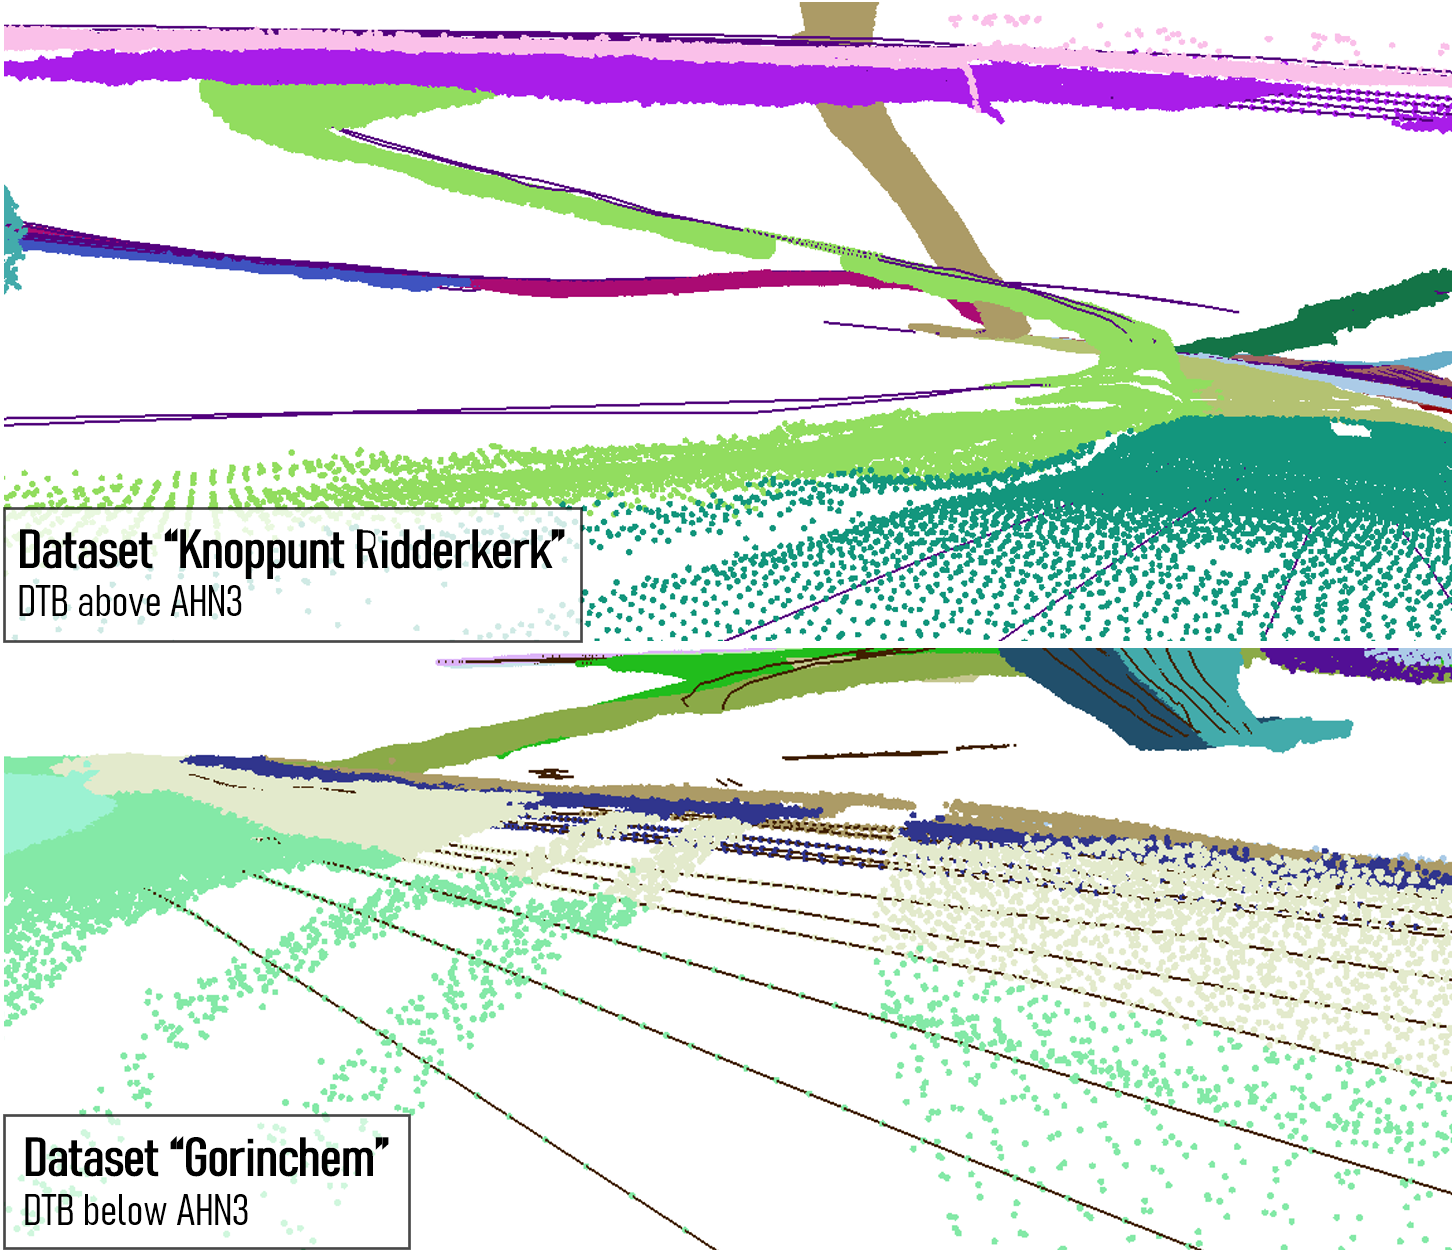
\includegraphics[width=0.9\linewidth]{final_report/figs/lidarsegmentation1.png}
    \caption[Renders showing the disagreement between AHN3 and DTB]{Visualisations illustrating the disagreement between \ac{ahn3} and \ac{dtb}. The symbology is the same as in Figure \ref{fig:lidarsegmentation0}.}
    \label{fig:lidarsegmentation1}
\end{figure}

\subsubsection{DTB's usefulness}

As discussed in-depth in Section \ref{sub:m_lidarsegmentation}, the final version of my code works well even in the presence of long occluded regions, even without \ac{dtb} coverage. However, \ac{dtb} is still used wherever available and useful. One clear benefit is that \ac{dtb} can help rectify plane fits, thereby segmenting \ac{ahn3} more accurately in the vicinity of the gaps. Often, this automatically fixes the outlier-related issue I mentioned above in the context of slightly corrupted plane fits just before and after data gaps.

Furthermore, even in the knowledge that \ac{dtb} is severely outdated in many places (see Section \ref{sub:dtb}), it is still the only information source we have about roads where \ac{ahn3} coverage is missing. Where the break in \ac{ahn3} coverage is short and \ac{dtb} is outdated (or missing), linear interpolation prevails. However, where longer gaps are present and the road's elevation may change inside of them, \ac{dtb} prevails even if its data its outdated.

Unlike in most locations, \ac{dtb} has good coverage in the particular motorway junctions shown in Figures \ref{fig:lidarsegmentation0} and \ref{fig:lidarsegmentation1}, especially in the \textit{Knooppunt Ridderkerk} junction. Each of the visualisations in these figures contain examples of how \ac{dtb}-based "assistance" manifests itself in the output. Where subclouds contain Lidar-gaps filled with points in a linear arrangement, one can be certain that \ac{dtb} was used to re-fit planes and to supply points to the subcloud. In the upper part of Figure \ref{fig:lidarsegmentation0}, these linear sets of points appear in the lowest motorway lanes and ramps wherever the 3 overlying roads cast "shadows" on it, creating occluded zones of various shapes. Each level of the stack of roads has such a feature, except for the one on the top, which is not occluded by any objects.

While this demonstrates that \ac{dtb} - or any support dataset with road surface elevation measurements - can be helpful in complementing this procedure (which is otherwise based entirely on \ac{ahn3}), it also highlights one of \ac{dtb}'s weaknesses. While the areas shown in these figures have good \ac{dtb} coverage, the \ac{dtb} lines in the \textit{Knooppunt Ridderkerk} dataset are in some cases approximately two decades older than \ac{ahn3} (they are up-to-date in \textit{Knooppunt Deil}). Figure \ref{fig:lidarsegmentation1} demonstrates that there are noticeable systematic differences between the road elevations as depicted by \ac{ahn3} and \ac{dtb}.

In \textit{Knooppunt Ridderkerk}, \ac{dtb} is above \ac{ahn3} consistently, but the \textit{Gorinchem} dataset and several others show \ac{dtb} \textit{below} \ac{ahn3}. Moreover, as the top visualisation in Figure \ref{fig:lidarsegmentation1} shows, perfectly and poorly matching \ac{dtb} and \ac{ahn3} data and can often be found side-by-side, with only a few years of difference between the \ac{dtb} acquisition times. While in Section \ref{sub:dtb} I primarily attributed these problems to the effects of subsidence, a further investigation of the problem is justified based on these results. The reasons for these differences may be more complex than simply just being the result of subsidence.

This issue draws our attention to the general issue of temporal discrepancies between all our datasets - \ac{nwb}, \ac{ahn3}, and \ac{dtb}. This is further discussed in Sections \ref{sub:r_tinconstruction} and \ref{sub:r_interpolation} in the context of how it affects our results. Overall, the results suggest that even if we solely attribute the vertical land motion to subsidence, a 20 cm verical accuracy can only be guaranteed by periodically re-measuring the input elevations in both the primary and the support datasets.

\subsubsection{Splitting NBRS into parts}

On the left in Figure \ref{fig:lidarsegmentation2}, a region with neither \ac{ahn3}, nor \ac{dtb} coverage is shown. In this location, the \ac{nbrs} was split into two parts and in the figure, this is illustrated by the fact that I could highlight the subcloud on one side of the gap separately. The matching colour of the points shows that they still belong to the same \ac{nbrs}, but the program stores a separate subcloud for each \ac{nbrs} part, meaning that they are loaded as a separate MultiPoint object in the 3D viewer I used to generate these figures. \ac{nbrs} splitting also works well in general, it performs as expected.

\subsubsection{Parametrisation}

The parametrisation of this pipeline step is extensive, because many parts of the algorithm are of a procedural nature. Hence, I will dedicate some attention here to describing the final parametrisation I used to produce my outputs. Here I will not go into details about the exact way in which these parameters are used, as I have already described this in Section \ref{sub:m_lidarsegmentation} without specifying numerical values.

All parameters were derived from a process of experimentation and fine-tuning, although a good understanding of the problem, the procedures, and the properties of the input data were also essential in being able to define the parameters as well as to find suitable values for them.

Firstly, a query radius for the generation of the Lidar patches needs to be specified. I used a query radius of 10 metres, which is sufficiently long to allow most of road surface reflections to be included between centreline vertices. Using a smaller radius could, in some cases, improve the plane fitting results, but it would also cause the exclusion of useful Lidar points from the patches simply due to the spherical geometry of the query regions. While the radial queries are not perfectly suitable for this step, I did not implement a custom query mechanism because the performance of the radial KD-tree queries is needed for this step. The performance of this querying step is also heavily affected by the vertex densification threshold and Lidar thinning factor used previously; denser \ac{nbrs} vertices and a denser input point cloud means that the processing time will increase considerably.

When the program examines the Lidar patches corresponding to each \ac{nbrs} vertex, it either fits a plane and passes on the patch, only passes on the Lidar patch, or does neither. The program stops fitting planes below 2 points per square metre, and stops passing on points below 1. In this context, "points per square metre" is interpreted rather loosely, since the patches are actually based on points falling into spheres of a given radius rather than circles. However, since Lidar points are assumed to have been reflected from a \textit{nearly} 2.5D surface locally, this assumption is not unreasonable.

The next set of parameters controls the detection of "instability" while examining the succession of plane fits and underlying Lidar patches. \ac{dtb}-based assistance is attempted if any of the following conditions are met: the standard deviation of the Lidar patch's elevations exceeds 0.1 metres, the distance between the plane and the corresponding \ac{nbrs} vertex grew by more than 50\% since the previous iteration, or the median of the Lidar patch's elevations grew by more than 50\% since the last iteration. The latter two conditions are only considered if the absolute value of the underlying metrics (distance from \ac{nbrs}, median elevation) exceeds 0.2 metres.

The way the metric related to the centreline-subcloud elevation differences is enforced ensures that the occasional poor polynomial fits of the previous step do not cause problems here. Such fits cause the centreline to underestimate or overestimate the elevation of roads in a consistent manner. Making the metric detect abrupt \textit{changes} in these distances rather than simply setting a distance threshold adds enough flexibility to bridge the issue.

When \ac{dtb}-based assistance (re-fitting of plane) is attempted, the initial query radius when looking for \ac{dtb} points is 0.4 metres. If enough points were found to re-fit the plane (more than 2), then the second repositioning query is performed with the same radius as the one used in the generation of the Lidar patches (10 metres in my final parametrisation), because at this point it is assumed that the query position has been moved relatively close to the true elevation of the road surface. When deciding whether to do a final re-fit on the nearby part of the Lidar patch, the program once again uses the condition that the density of these points should at least be 2 points per square metre. Lidar points are deemed to be close if they are less then 1 metre away from the plane.

When pre-selecting the final set of conformant points from the patches, the program uses a threshold of 5\% of the query radius used in the Lidar patch queries, corresponding to 0.5 metres (from the final plane fit) in my final parametrisation. Outliers that are further away than 0.5 m from the subclouds do not violate this condition, they simply indicate that the underlying plane fit was somewhat tilted relative to the road surface.

While the post-processing operations of this pipeline step (breaking into \ac{nbrs} parts and filtering outliers) also have a few parameters, these are insignificant and are thus omitted from this discussion.

\begin{figure}
    \centering
    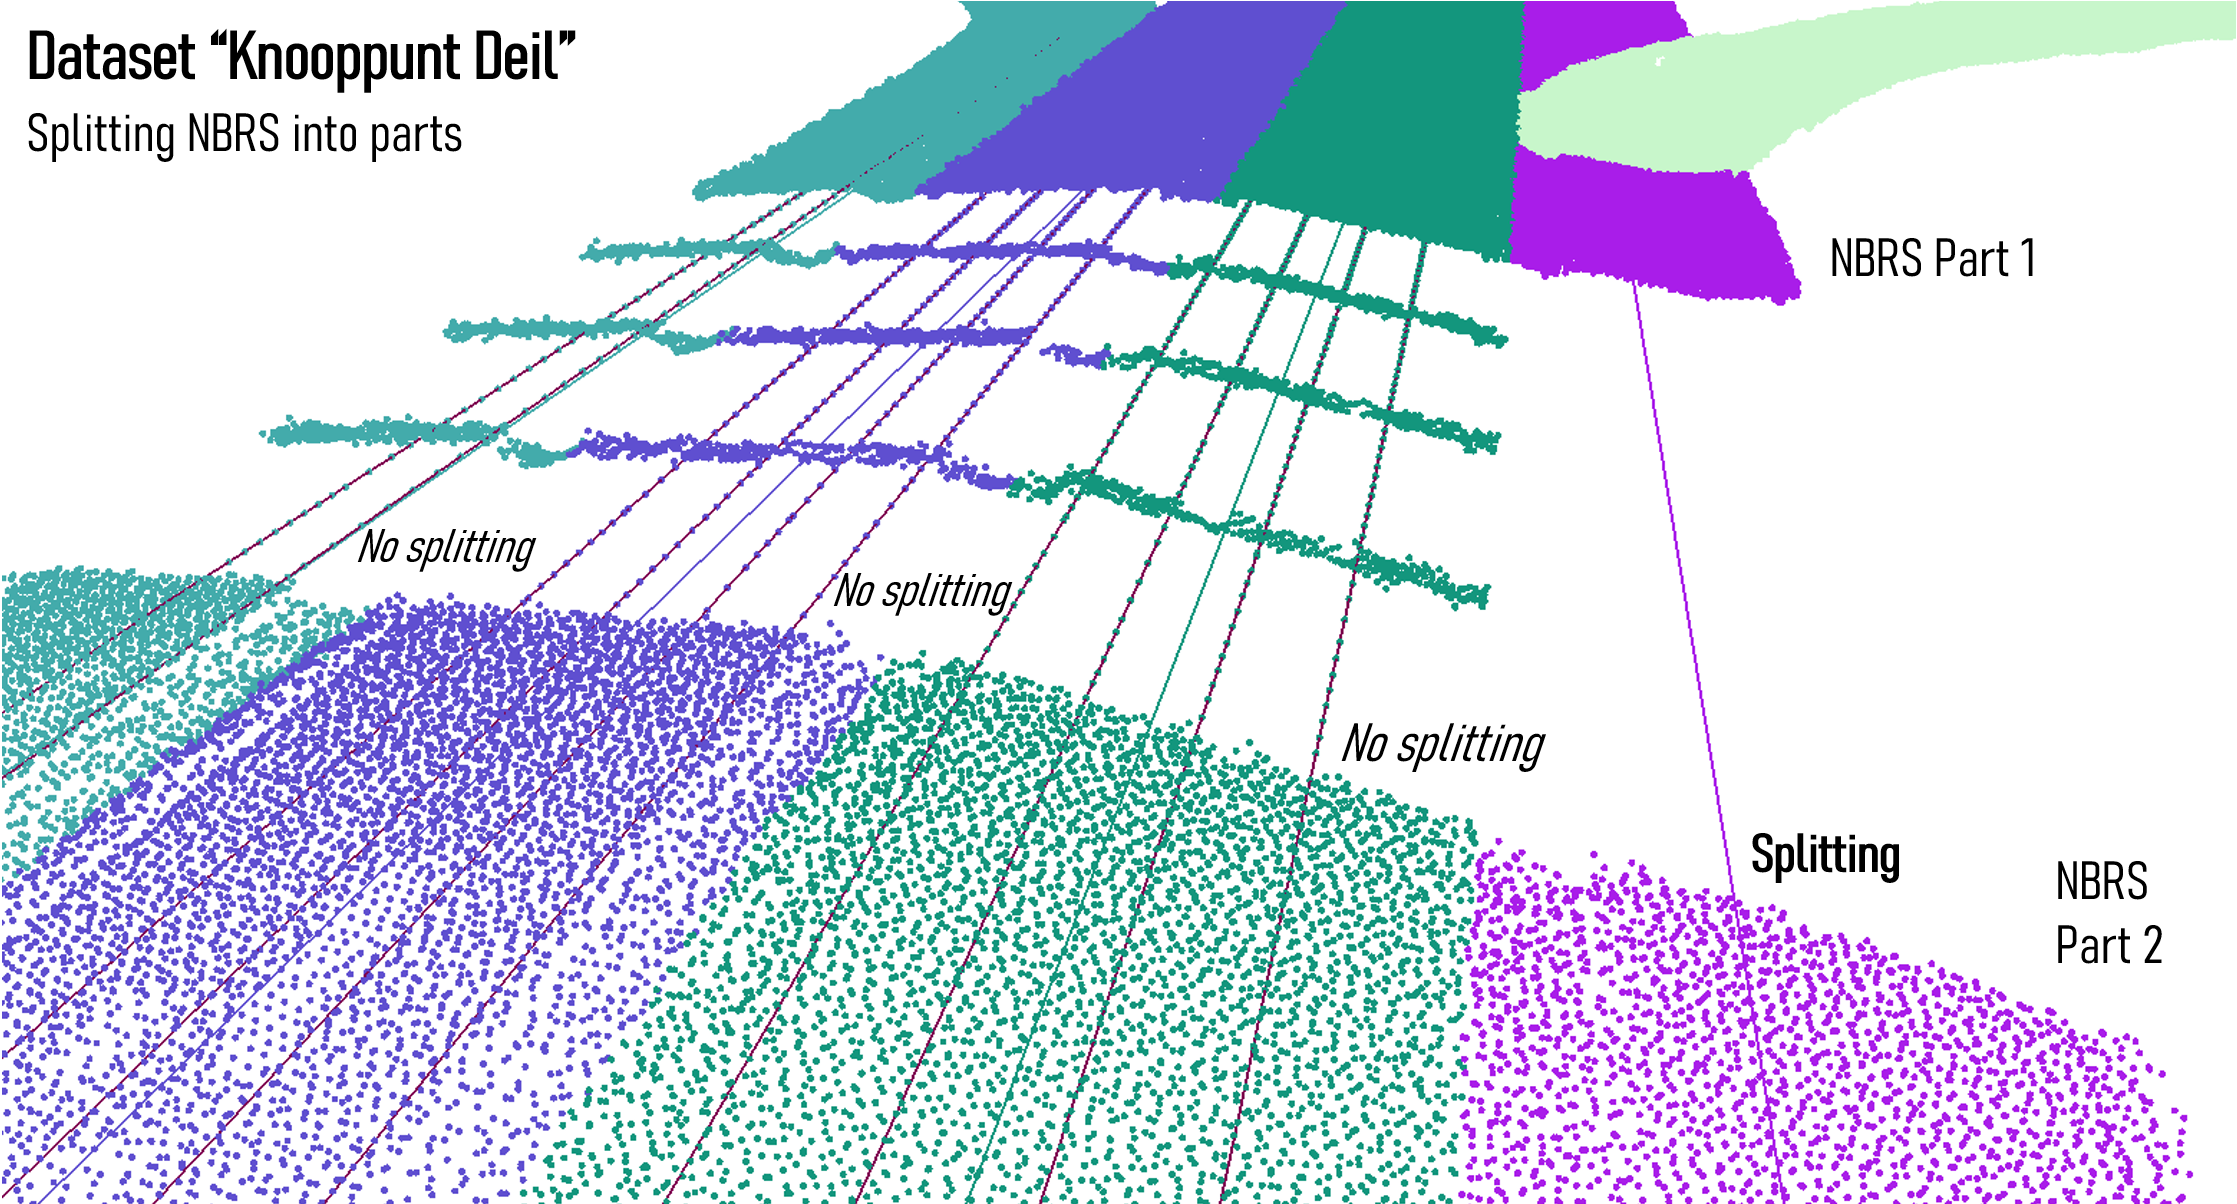
\includegraphics[width=0.92\linewidth]{final_report/figs/lidarsegmentation2.png}
    \caption[Render illustrating the handling of AHN3 gaps during Lidar segmentation]{Visualisation illustrating the handling of gaps in \ac{ahn3} coverage during Lidar segmentation. The colour-coding of the 3D NBRS lines and the subclouds was randomly generated based on their NBRS IDs. The relevant DTB lines are shown in dark red, where available.}
    \label{fig:lidarsegmentation2}
\end{figure}

\subsubsection{Using the implementation}

The below code snippet shows the code I used to generate my final results.

\begin{verbatim}
roads.segment_lidar(fpath = dtb_fpath, r = 10)
roads.write_subclouds(fpath = subclouds_fpath)
\end{verbatim}

The first line performs the point cloud segmentation itself, with a radius of 10 metres for the KD-tree queries that generate the Lidar patches. The variable \codeword{dtb_fpath} is assumed to contain the file path to the cropped \ac{dtb} file belonging to the desired testing dataset. The second line writes the resulting subclouds to disk, the argument variable is assumed to contain the file path to the desired output file.

The intermediate results that the second line writes to disk "mimics" the structure of the input LAS file. However, each point is given three new properties. The property \codeword{ORIGIN} determines whether the given point originates from \ac{ahn3} (denoted by the value \codeword{0}) or \ac{dtb} (denoted by the value \codeword{1}). The properties \codeword{NBRS_ID} and \codeword{PART_ID} determine which \ac{nbrs}, and which part of that \ac{nbrs} a given points belongs to. \ac{nbrs} that were not split into parts are still represented by the same data structure, but all their points are found in a single part with \codeword{PART_ID = 0}.

In the class itself, the resulting subclouds can be accessed via \codeword{.nbrs_subclouds[nbrs_id][part_id]}, where \codeword{nbrs_id} and \codeword{part_id} are variables which should contain the ID of a specific \ac{nbrs}, and the ID of one of its parts respectively. Furthermore, one can find the indices corresponding to intervals with \ac{ahn3} or \ac{dtb} coverage in \codeword{.nbrs_parts[nbrs_id]}, which effectively defines the \ac{nbrs} parts in the software.

\subsection{Edge approximation}
\label{sub:r_edgeapproximation}

Visualisations showing the results of the edge approximation step are shown in Figure \ref{fig:edgeapproximation0}. The black lines correspond to \ac{nwb} centrelines, while the closely spaced, orthogonal lines are the cross-sections that are attempted to be created on each centreline vertex. The lines connecting the ends of the cross-sections on each side of each centreline are the preliminary edges that are the main product of this processing step. As in all 3D visualisations in this chapter, the vertical dimension is once again exaggerated five times to make vertical changes better visible.

\subsubsection{General description of results}

The output of this step is mostly satisfactory, no road layouts apart from tunnels are known to me which would cause the algorithm to fail, or produce unusable results with the final parametrisation. Furthermore, owing to the verification step that takes place before accepting a cross-section (and extending the preliminary edge with its end vertices), the general shape of the edges is also quite well-behaved, and their elevation reflects what one would expect based on the underlying subclouds. In my final configuration, cross-sections have vertices every 10 centimetres (created via densification), and their elevation is derived from points no further than 25 centimetres away. This dense quantisation allows the algorithm to reconstruct road edges on a fine scale.

\begin{figure}
    \centering
    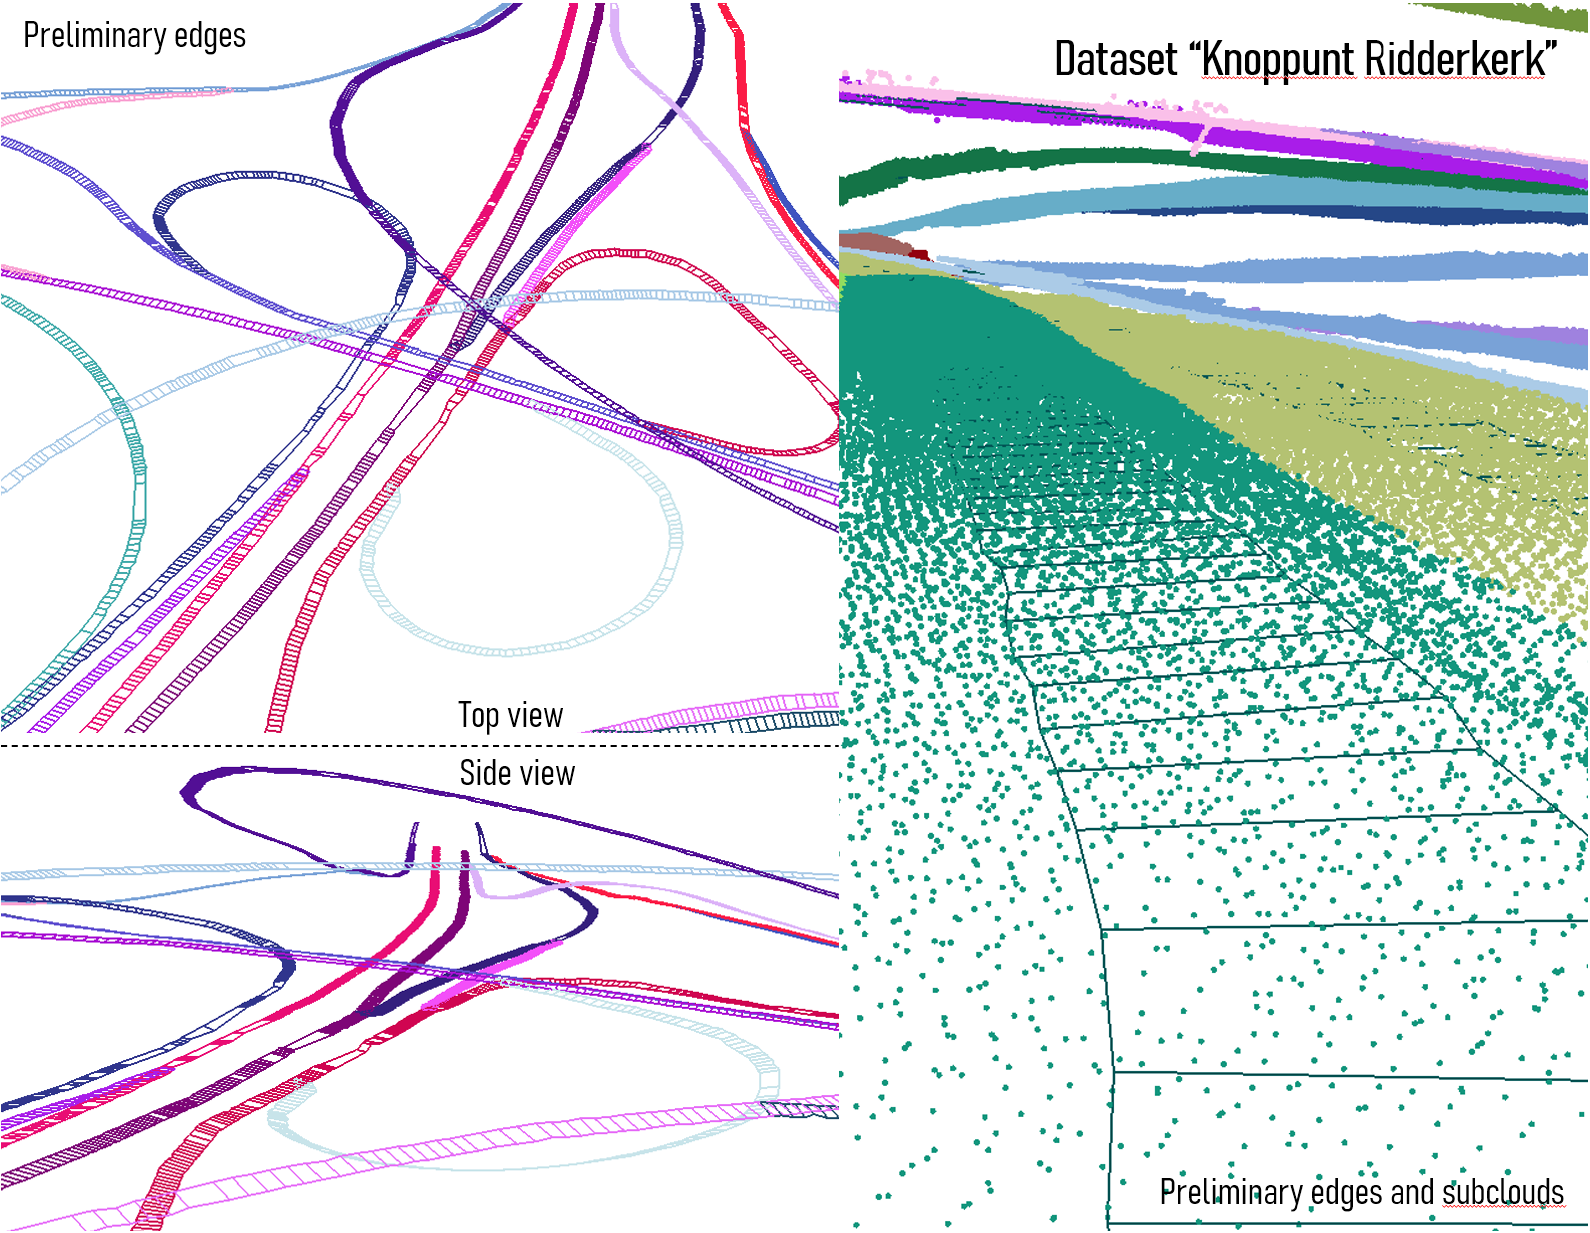
\includegraphics[width=0.9\linewidth]{final_report/figs/edgeapproximation0.png}
    \caption[Renders illustrating the results of preliminary edge approximation]{Renders illustrating the results of preliminary edge approximation. Left: visualisations showing the generated preliminary edges and cross-sections. Right: visualisation comparing the edges and cross-sections to the underlying subclouds. The edges, cross-sections and subclouds are coloured randomly based on their NBRS IDs.}
    \label{fig:edgeapproximation0}
\end{figure}

In the two visualisations on left in Figure \ref{fig:edgeapproximation0}, I visualised the preliminary edges only. The top image looks down on \textit{Knooppunt Ridderkerk} from above, while the one below shows the same roads from the side. On the right in the figure, I show a visualisation in which a pair of preliminary edges and the underlying cross-sections can be compared with the subcloud that was used to generate them. In most cases, cross-sections and preliminary edges lie flat on road surfaces, and even where noticeable blunders are observed, they correspond to underestimating or overestimating the road surface extents by about 2 metres maximum.

While the overall quality is good and the results are certainly usable in terms of the requirements of the next two pipeline steps, there are a few properties and limitations of these results that are worth discussing.

\subsubsection{On road width bounds}

As I already mentioned in Section \ref{sub:m_edgeapproximation}, the algorithm works with a fixed minimum and maximum road width. The maximum is enforced by using it as the length of the constructed cross-sections, while the minimum is enforced as part of the verification step.

The enforcement of the minimum width is less of a limitation; it merely prevents the cross-sections from shrinking too short. However, the the way in which the maximum width is enforced can be considered a limitation because road surfaces that are unusually wide will not be covered by the edges in their entirety. Using very long cross-sections (increasing the maximum width) increases the chances of returning false hits due to short successions of off-road points that conform well with the line fits of the cross-sections. With shorter cross-sections, the chances of this happening are reduced drastically.

My final parametrisation uses minimum and maximum road widths of 3.5 and 7 metres respectively.

While the maximum limit may exclude meaningful road surface areas in the case of unusually wide roads, there are special roads in which road and off-road reflections are not clearly distinguishable in the cross-sections. Motorway lanes are represented by discrete centrelines in \ac{nwb}, which means they will be treated as separate \ac{nbrs} in my system. However, such lanes are often constructed on a single paved surface, meaning that my method cannot be used to derive edges at least for one side of them. This is another reason why the maximum width is important; one such scenario is shown on the left in Figure \ref{fig:edgeapproximation1}.

It is primarily \ac{nwb}'s crude georeferencing that necessitates the use of a lower-than-optimal value for the maximum road width. If \ac{nwb} itself is shifted towards the edge of a road locally, generated cross-sections will be corrupted there by off-road elevations. Using larger values for the maximum width will only make this problem worse. In the absence of this problem, the value could be increased by a few metres based on my experience with accurate parts of \ac{nwb}.

I implemented a workaround that mitigates the effects of this issue. The line fits that are generated for every cross-section are actually only fitted on the central 40\% of the densified cross-section vertices, and it is extrapolated to the outer vertices. This helps minimise the effects of the off-road elevation measurements that may affect the outer cross-section vertices. 

\subsubsection{Failed edge detection}

\begin{figure}
    \centering
    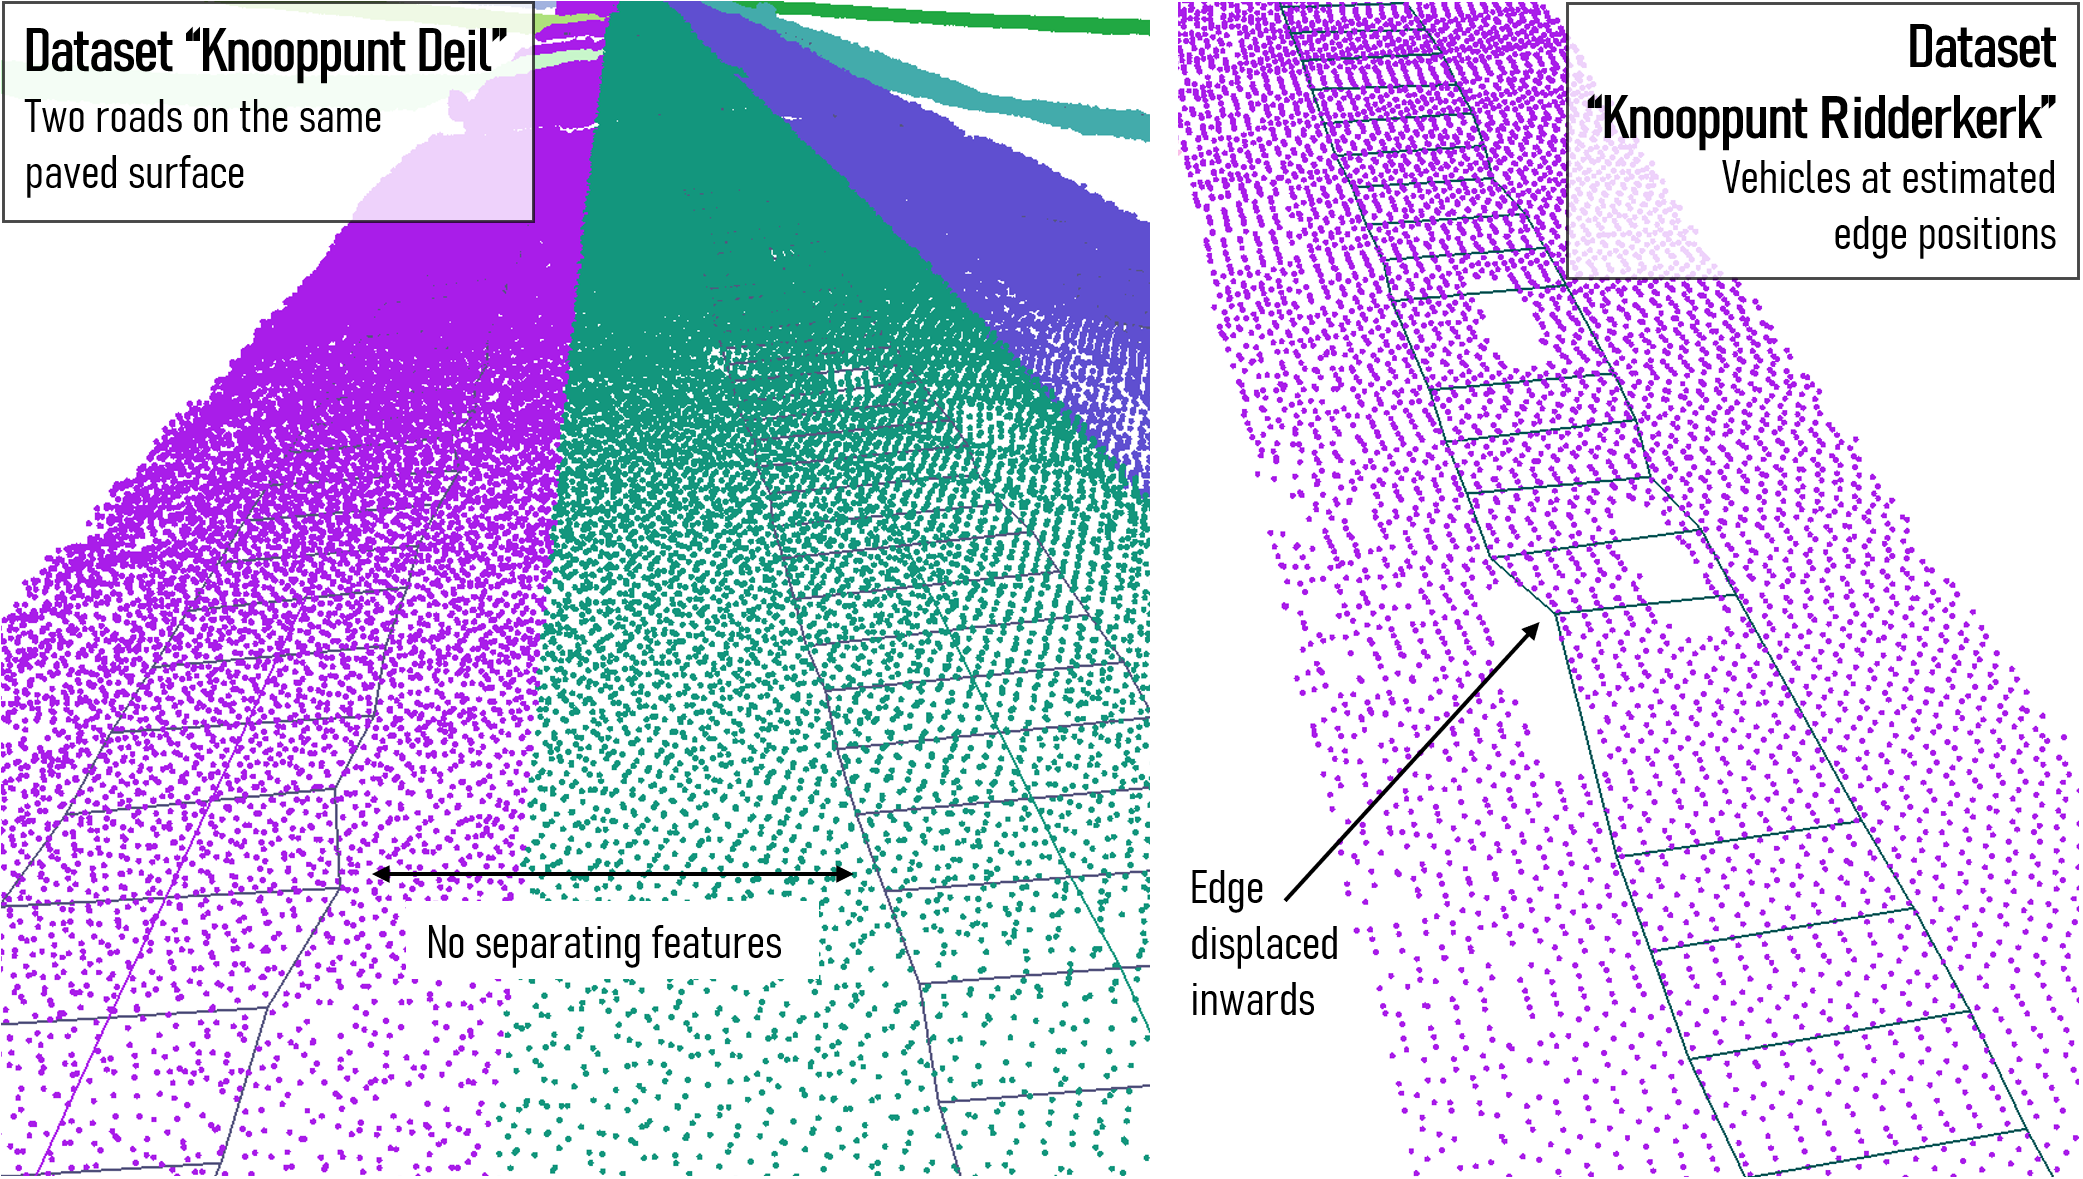
\includegraphics[width=\linewidth]{final_report/figs/edgeapproximation1.png}
    \caption[Renders illustrating challenging edge approximation scenarios]{Visualisations illustrating challenging edge approximation scenarios. The preliminary edges and cross-sections are shown as dark lines, and the subclouds are coloured randomly based on their NBRS IDs. One the left, the relevant preliminary 3D-NWB centrelines are also shown in the same colour.}
    \label{fig:edgeapproximation1}
\end{figure}

While in well-exposed, straight roads this does not generally happen, there are lengths of roads where finding edge points will fail repeatedly. In such places, the algorithm does not save the cross-sections, and also does not add edge points to the preliminary edge LineStrings. One the left in Figure \ref{fig:edgeapproximation0}, this can be clearly observed, as it occurs frequently in occluded areas.

The most common reason for skipping cross-sections is the lack of data. If not enough Lidar points are found close to the cross-section vertices, then it will be skipped. This happens in data gaps where both \ac{ahn3} and \ac{dtb} are missing, but \textit{also} in most gaps where \ac{dtb} is available. The latter is due to the fact that \ac{dtb} samples linear features \textit{along} the length of each road, and has a poor sampling rate in the direction that the cross-sections are attempting to sample.

Such data gaps may exist under bridges for instance, but also in places where vehicles occluded a significant portion of the road. In the latter case, artefacts may be generated if the cross-sections are accepted because there is enough data not to trigger a skip. Most commonly, it causes noticeable width changes, which may be accepted by the algorithm if the relevant cross-section is processed while the conditions are relaxed due to repeated previous failures. This is shown on the right in Figure \ref{fig:edgeapproximation1}.

The second most common reason is the generation of poor line fits. If the elevation estimates of the cross-section vertices are scattered, the errors in the fit will be large. Elevations further than one standard deviation of the data-model error are not considered any further. If too many points are filtered out in such a way, the cross-section will be skipped. This happens most commonly due to \ac{nwb}'s poor georeferencing, i.e. in the rare cases when not even only using the central 40\% of the cross-section vertices could avoid including a large number of off-road elevation measurements.

Lastly, failures may also be the result of violating the conditions of the verification step. Namely, if a unrealistically sudden width or elevation change is detected, the cross-section is skipped. If this is the sole reason for the failures, then generally only a limited number of cross-sections and corresponding edge vertices will be missing, as the conditions are relaxed after 3 successive failures.

\subsubsection{Edge generation in data gaps}

In the absence of \ac{ahn3} data, vertices will be skipped frequently, as I already mentioned above. However, quite frequently, one or two cross-sections will be accepted in such regions too, if \ac{ahn3} coverage reappears temporarily, for instance due to a small gap between two bridges. Due to the repeated skipping of vertices, the conditions will almost certainly be relaxed most of the time, and hence sudden width or elevation changes will be allowed. This combination of factors may result in the generation of strange edge geometries in occluded zones.

Where roads are straight and the gaps in coverage are short, this does not represent a major issue. Even if their shape will be sub-optimal in these zones, it will still respect the minimum road width condition, meaning that most \ac{dtb} and \ac{ahn3} points that may appear in the gap will still fall between the edges, which is ideal for \ac{tin} construction.

Serious problems only arise when the gap appears at the end or the beginning of an \ac{nbrs} part. In such cases, especially if there is no intermittent \ac{ahn3} coverage in the gap, no cross-sections will be accepted at all, and therefore the program will be unable to extend the edges to the end of the \ac{nbrs} part. The beginning or the end of the centreline will simply not be covered. Later in the \ac{tin} construction step, this means that the local \ac{dtb} points will not be inserted into the \ac{tin} (because they are not between the generated edges), and the \ac{tin} surface will, as a result, also not extend all the way to the end of the \ac{nbrs} part. This directly introduces incorrect (linearly interpolated) elevations to the final 3D-NWB output.

A similar problem arises when a road is occluded in a bend. Depending on the sharpness of the bend and the extent of the occlusion, the preliminary edges may end up directly connecting the last cross-section before the occlusion and the first one after. Taking such a "shortcut" means that \ac{dtb} points in the data gap will mostly be ignored during \ac{tin} generation because they will not fall between the preliminary edges.

I have not observed the above limitations to cause issues with roads that are built on the surface in practice. However, they do mean that my system design is not compatible with tunnels out-of-the-box. Unless the tunnel is completely straight and the relevant \ac{nbrs} part continues across its full length, the \ac{dtb} points in the tunnel will be ignored during \ac{tin} construction, and therefore the \ac{tin} models and the 3D conversion of \ac{nwb} will be incorrect locally. I tested and verified this issue with the \textit{Amsterdam Hemhavens} and \textit{Amsterdam Zuid} testing datasets, which both contain tunnels.

As I noted in Section \ref{sub:dtb}, I treat \ac{dtb} as a "placeholder" for a better supporting dataset (optimally, an \ac{mls} dataset). As a result, its vector properties are not used - it is assumed to consist of generic point data. However, treating it properly as a 3D line dataset in \ac{ahn3} data gaps would fix the above issues, i.e. it would become possible to generate edge estimates from \ac{dtb} much like in the commercial implementation. Such an extra feature did not fit into the schedule of my project, hence it is only further discussed in the Future work section in the Conclusions chapter (see Section \ref{sec:futurework}).

\subsubsection{Using the implementation}

In my example code on GitHub, I use the following two lines to generate and export the preliminary edges:

\begin{verbatim}
roads.estimate_edges(min_width = 3.5, max_width = 7, thres = 1, perc_to_fit = 0.4)
roads.write_edges(fpath_edges = edges_fpath, fpath_crosses = crosses_fpath)
\end{verbatim}

The first line generates the preliminary edges. The arguments (all compulsory) set the minimum and maximum road width, the outlier filtering threshold, and the ratio of how much of the cross-sections should be fitted with lines. The first two arguments should be specified in metres. The second argument specifies the number of standard deviations of data-model errors, within which points should be considered inliers, so the current value means one standard deviation. The last argument accepts values between 0 and 1, the current value means that the central 40\% of cross-sections will be used as the basis for the line fits.

The second line writes the results to disk. Both the edges and the cross-sections are written, \codeword{edges_fpath} and \codeword{crosses_fpath} are assumed to contain file paths where these should be written (as Shapefiles). In the class itself, the results are found in \codeword{.nbrs_edges} and \codeword{.nbrs_crosses} as GeoDataFrame objects.

\subsection{Active contour optimisation}
\label{sub:r_activecontours}

As Figures \ref{fig:activecontouroptimisation0} and \ref{fig:activecontouroptimisation1} show, all planned parts of this pipeline step output the expected results, albeit with occasional artefacts and a mediocre overall quality. The contours are smooth, they generally reflect the shape of the roads accurately, and only occasionally suffer from major blunders. However, even small deviations beyond the road edges would cause off-road Lidar reflections to be classified as road points, and thus be inserted in the \ac{tin} model in the next step. Unfortunately, such deviations of various sizes occur frequently, as the close-up images in Figure \ref{fig:activecontouroptimisation1} demonstrate. With the help of the results, this section will focus on explaining why exactly it is difficult to guarantee that this workflow functions reliably, as this was the reason for a major revision of the design of the preliminary edge detection and \ac{tin} construction steps, which I already mentioned in Section \ref{sub:m_edgeapproximation}.

\begin{figure}[h]
    \centering
    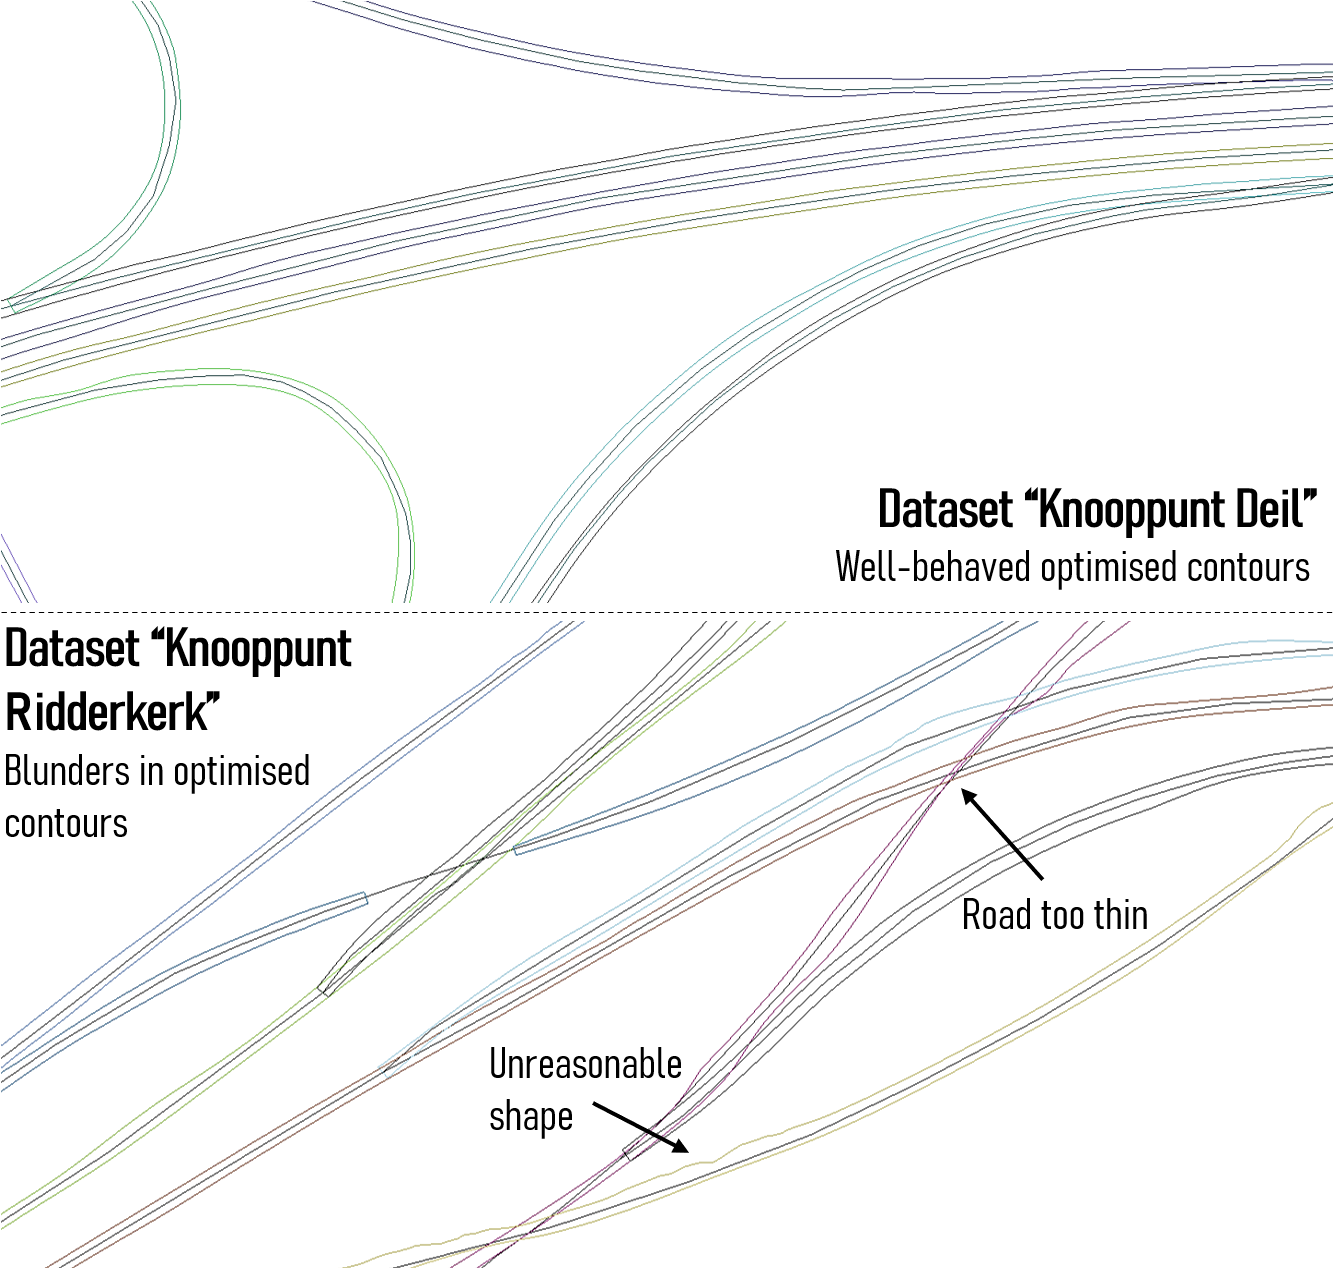
\includegraphics[width=0.84\linewidth]{final_report/figs/activecontouroptimisation0.png}
    \caption[Renders illustrating the results of active contour optimisation]{Visualisations illustrating various degrees of active contour optimisation success. In these 2D visualisations, NWB is shown as dark grey lines, whereas the optimised edges are coloured randomly based on their NBRS IDs.}
    \label{fig:activecontouroptimisation0}
\end{figure}

\subsubsection{Attractor maps}

Some attractor maps can be seen in Figure \ref{fig:activecontouroptimisation1}. Each \ac{nbrs} part has its own attractor map, and since subclouds may overlap, so can the attractor maps. In the figure, attractor maps that are separated from others by a fair amount of distance can be examined in their full width, while only the one the was drawn last by the visualisation software can be examined completely where overlapping occurs.

The bright parts of the attractor maps correspond to regions were the normal vectors of the Lidar points are oriented uniformly, while the darker regions indicate divergent normal vectors. The linear boundary between such regions thus marks the edge of the smooth road surface in most places, as it corresponds to an abrupt increase in normal vector divergence. I used a pixel size of 0.5 metres (in both dimensions) to generate these attractor maps, and the attractor map values are based on using a 5-by-5 kernel, sampling the neighbourhood via approximately 30 inner products for each pixel.

The optimised contours are shown overlain on the attractor maps on the right in Figure \ref{fig:activecontouroptimisation1}. While the \textit{general} appearance of the contours is acceptable, comparing \textit{details} in the contours with the attractor maps reveals that they are not reliably positioned on the break in smoothness. So that the reader can better interpret the optimisation as a process, the left part of Figure \ref{fig:activecontouroptimisation1} shows the preliminary edges overlain on the attractor maps. Comparing the preliminary edges to the contours in the context of the attractor maps allows one to better understand the effects of the optimisation procedure. In particular, patterns in the behaviour of the optimisation procedure may be recognised.

\subsubsection{Patterns of failure}

One important pattern is that the contours are sensitive to small-scale features in the preliminary edges. A few outlier edge points (an short, abrupt expansion of the preliminary edges, for instance) can introduce large bulges into the optimised edges. Similarly, where the preliminary edges shrink (for instance due to the influence of stationary vehicles), the optimised contours will tend to do so too, but on a much larger scale. The severity of the generated artefacts also depends on the local properties of the attractor maps.

Another pattern, which I already mentioned in \ref{sub:m_activecontours}, is that where preliminary edges fall outside the bright part of attractor maps, the the optimisation procedure will often fail to move them back to the primary break in smoothness. The off-road areas may contain other high-contrast features due to the unevenness of the underlying real-life surfaces, and the edges will often be drawn to these instead of the edge of the road. This is in part due to the large weight the optimisation algorithm gives to the \textit{proximity} of the edges.

For the same reason, deliberately underestimating the road width (which was done in \cite{boyko_funkhauser_2011}) does not represent a solution here. If the preliminary edges are too far inwards from the break in smoothness, they will simply stay unchanged during optimisation. This behaviour cannot be changed simply via the parametrisation - I already give nearly full weight to edge detection in my final configuration. I also experimented with underestimating the preliminary road widths and giving more weight to attraction to darkness. Unfortunately, the results of this approach are even more unpredictable because the algorithm will frequently move the contours into the dark areas rather than stop at the edges.

Lastly, the contours may also become corrupted due to the break in smoothness itself missing from the attractor maps. The two most common factors that tend to cause this are unusually wide paved surfaces (wider than the maximum width of the underlying subcloud), and occluded zones where only \ac{dtb} is available. The former is manifested in the attractor maps by the bright zone extending all the way to the edge of the map. In such regions, active contour optimisation will leave the preliminary edges mostly unchanged (there are no edges to attract it). The latter (missing \ac{ahn3} coverage) may cause unpredictable artefacts because the edge needs to step into the no-data region and then back into the road surface on the other side, transgressing two "edges" that are orthogonal to its general direction. Using a no-data value that is almost the same as typical road surface pixel values helped, but it could not solve the issue completely. Only by splitting \ac{nbrs} into parts here too, could this issue be eliminated.

Finding a suitable value for no-data pixels required some experimentation. I found it most effective to set all no-data pixels to a value close to the values seen in bright road surface areas. So, in addition to the occluded areas, all other parts of the rectangular rasters are set to this value (specifically, a value of 1). While this creates artificial high-contrast edges in the attractor maps at the boundaries of the underlying subclouds, the preliminary edges do not get drawn to them because they are almost always much closer to the edge introduced by the edge of the road.

\subsubsection{Active contour optimisation parameters}

The $\alpha$ parameter controls lengthwise shrinking. I set it to a value of zero to indicate that this behaviour is undesired. In theory, the optimisation procedure introduces length changes into the contours naturally, by adjusting their shape. In theory, $\alpha$ should therefore be set to a small, but nonzero value to allow this behaviour. In practice, I found that this affects the results negatively.

The parameter $\beta$ controls the smoothness of the resulting contours, which can also be intuitively though of as controlling the tension of the underlying splines that active contour optimisation repeatedly fits. I set this value to 0.01, which in my experience corresponds to medium tension. Based on the testing I have done, smoothing the preliminary edges is one task in which active contour optimisation excels; it can eliminate small-scale protrusions that are generally meaningless, and can thus be considered noise. This in turn helps minimise the impact of the types of small-scale issues I already described above by keeping the contour relatively tense across them. 

The parameter \codeword{w_line} controls attraction to dark or bright pixel values. The attractor maps that I described above have a sharp contrast between the brightness of off-road pixels (which are dark), and road pixels (which are bright). However, this contrast is localised to the edges of the roads, and any amount of attraction to either dark or bright areas would draw the contour deeper into that region rather than keep it on their boundary, both in theory and in practice. In my final implementation, it is set to 0.05 to introduce a very small amount of attraction to bright areas, so that the contours are more likely to stay on the inner side of the road edges rather than go past them.

Thus, attraction in my recommended parametrisation is controlled almost entirely by edge detection (parameter \codeword{w_edge}). I set it to 1, meaning that the iterative refinement of the contours will be be governed primarily by attraction to edges, for reasons I already discussed above.

\begin{figure}
    \centering
    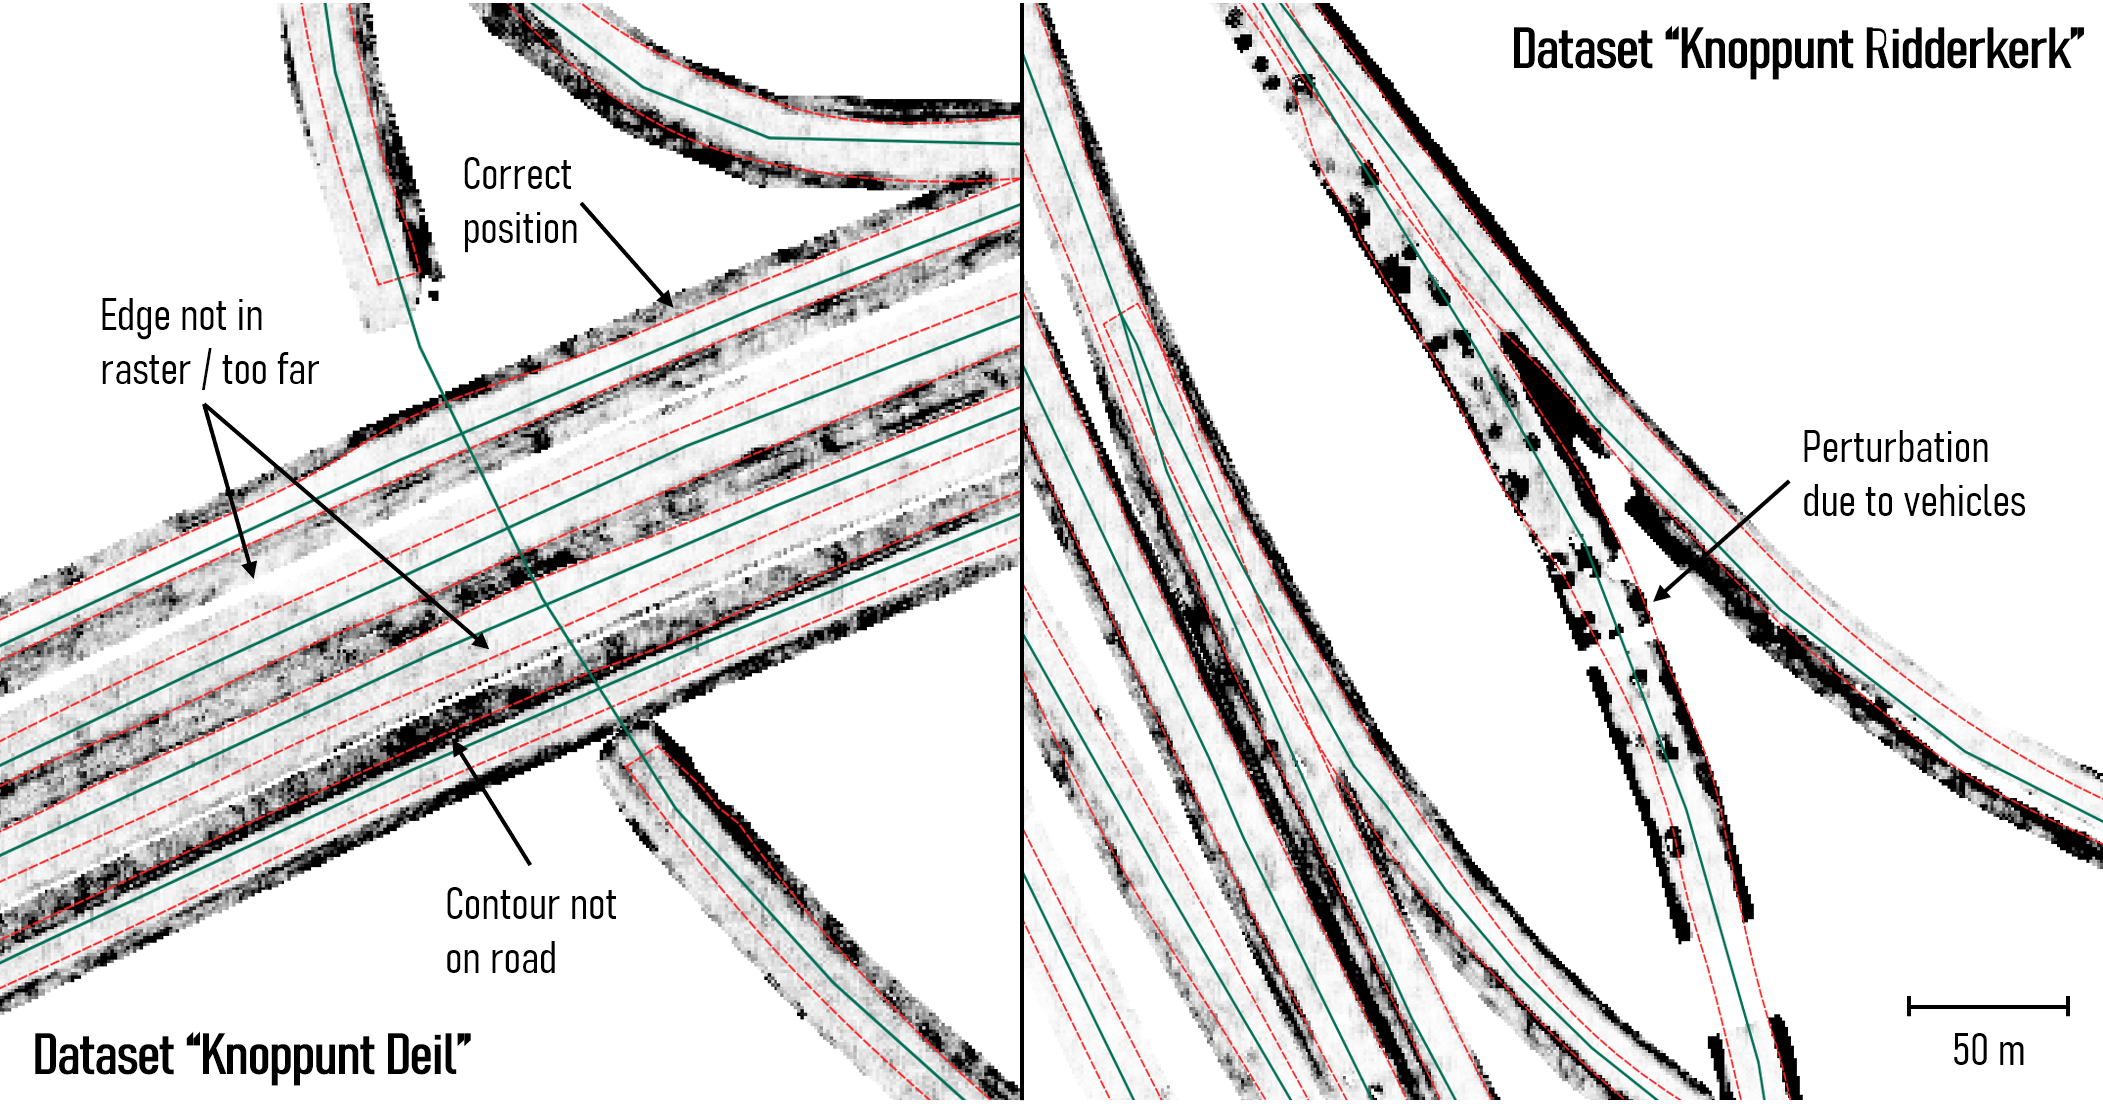
\includegraphics[width=\linewidth]{final_report/figs/activecontouroptimisation1.png}
    \caption[Visualisations comparing optimised edges to attractor maps]{2D visualisations comparing optimised edges to the underlying attractor maps. The attractor maps contain a single band with scalar values, hence they are shown visually as greyscale rasters. The NWB centrelines are shown in dark green, and the optimised contours as dashed red lines.}
    \label{fig:activecontouroptimisation1}
\end{figure}

In terms of iterations, I decided to work solely with a maximum number of iterations (parameter \codeword{max_iterations}) rather than to use condition-based termination. Setting a condition would terminate the optimisation process when the contours no longer move significantly, i.e. it checks when a minimum displacement threshold first becomes violated. Where the attractor maps are perfectly suitable for active contour optimisation, this approach works well. However, letting the contours evolve in such a way where the attractor maps are sub-optimal results in the drastic enlargement of the generated artefacts, as well as an unacceptable increase in computational complexity. This happens, for instance, where edges are not defined well enough, and where Lidar gaps are present. I found iteration limits between 1000 and 5000 to be the most effective.

The time step parameter $\gamma$ and the number of pixels the contours are allowed to shift in a single iteration (parameter \codeword{max_px_move}) can be used to further fine-tune how quickly the optimisation lets the contours evolve. I set these two values to 0.005 and 1 respectively, which corresponds to a relatively slow iteration, appropriate to the small-scale changes we desire (generally, we wish to move the edges only by up to a few metres.

The above configuration of values is the result of a process of iterative combined revision of the values themselves, and the attractor map generation technique, as I mentioned in Section \ref{sub:m_activecontours}. While I experimented with a wide range of parametrisations, the possibility remains that a better one exists. The parameters themselves offer many permutations to try, and the fact that the preliminary edge and attractor map generation also affects the results only increases the range of possibilities.  

However, despite having tried most types of parameter configurations and many different adjustments to the preliminary edges and attractor maps, I was unable to find a configuration that produces satisfactory results within the development time reserved for this step. The quality of the optimised edges is simply not good enough to be used to classify Lidar points reliably based on them. The situation was made worse by the fact that the combined computational complexity of generating high-resolution attractor maps and of using the optimisation algorithm made the refinement procedure a rather difficult and time-consuming task. This is what lead to my decision to instead focus on improving the quality of the preliminary edges and use them directly in the \ac{tin} construction step. 

\subsubsection{Choice of algorithm}

Contributing to the above uncertainty regarding the effectiveness of active contour optimisation is the fact that in relevant literature (e.g. \cite{boyko_funkhauser_2011}), mentions of its ineffectiveness relative to more sophisticated algorithms is made. My hypothesis was that with a sufficiently good pre-selection of Lidar points and pre-processing of attractor maps, conventional active contour optimisation could still work well, but this appears not to be the case in practice.

Lesser known, but more sophisticated offshoots of active contour optimisation exist, but have no open-source Python implementations. One such example is the "ribbon snakes" method. Considering the volume of further tasks in this project, I opted not to attempt to implement it based on first principles, especially considering that their superiority is not clearly demonstrated in relevant literature. They, too, are prone to producing artefacts of various types, even if they perform slightly better than conventional active contour optimisation.

\subsubsection{Using the implementation}

The following lines of code may be used to run active contour optimisation and export the attractor maps and resulting optimised edges:

\begin{verbatim}
roads.optimise_edges(size = 0.5,
                     a = 0, b = 0.01, g = 0.005,
                     w_l = 0.05, w_e = 1,
                     max_iter = 1000)
roads.write_maps(fpath = maps_fpath)
roads.write_contours(fpath = conts_fpath)
\end{verbatim}

The first argument \codeword{size} in the active contour optimisation method corresponds to the desired pixel size. The rest of the parameters expose some of the active contour optimisation parameters that I found the be useful for making smaller changes to the algorithm's behaviour. The arguments \codeword{a}, \codeword{b} and \codeword{g} correspond to $\alpha$, $\beta$ and $\gamma$ respectively, while \codeword{w_l} and \codeword{w_e} correspond to the two parameters controlling attraction to brightness and edges (\codeword{w_line} \codeword{w_edge} respectively). The last parameter sets the maximum number of iterations.

The \codeword{.write_maps(maps_fpath)} method writes all attractor maps generated (one per \ac{nbrs} part) as GeoTIFF rasters, tagging the file name with the relevant \ac{nbrs} ID and part ID. Hence, the argument file name is expected to correspond to the first part of the file name only, e.g. \codeword{.../C_39CZ1_map} would work. Reserving a separate folder for these is recommended. The contours are written as a single Shapefile.

In the class, the maps can be found in the variable \codeword{.nbrs_maps[nbrs_id][part_id]}, while \codeword{.nbrs_contours} contains the contours in the form of a GeoDataFrame.

\subsection{TIN construction}
\label{sub:r_tinconstruction}

\begin{figure}
    \centering
    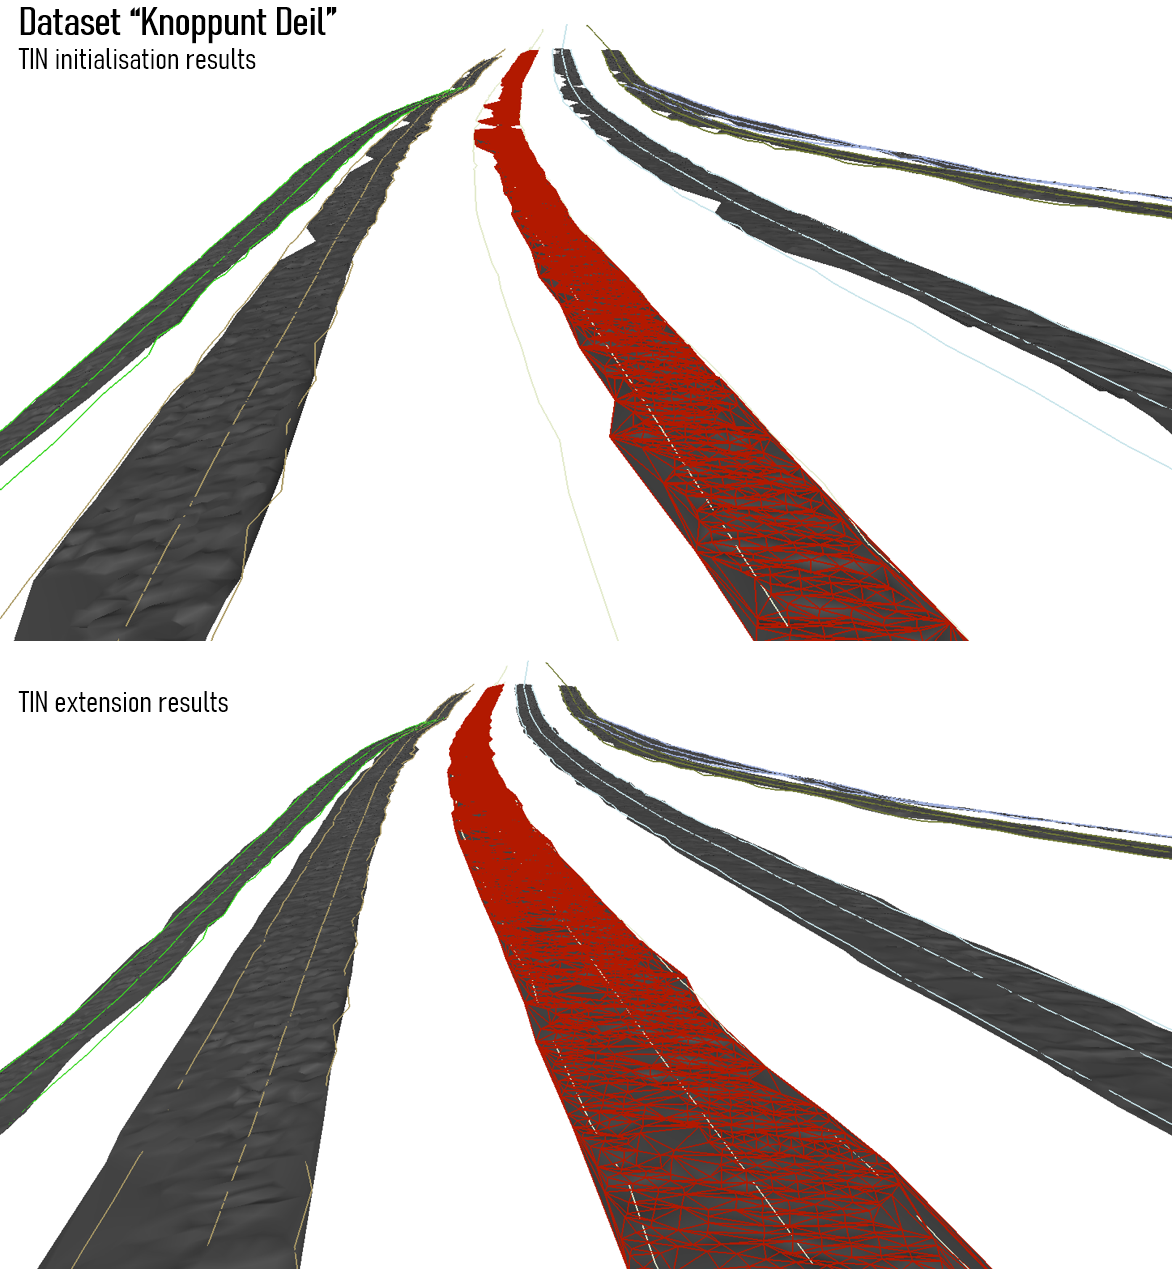
\includegraphics[width=\linewidth]{final_report/figs/tinconstruction0.png}
    \caption[Renders illustrating the results of TIN initialisation and extension]{Visualisations illustrating the results of \ac{tin} initialisation and extension. The TIN surfaces are shaded in gray, and the preliminary 3D-NWB and edge geometries are coloured randomly, based on their NBRS IDs. The triangulation of one of the TINs is shown as a red wireframe.}
    \label{fig:tinconstruction0}
\end{figure}

By adjusting my methods to the circumstance of not being able to produce accurate enough optimised edges, I created a different implementation than originally planned, but one which is still robust and accurate. Figures \ref{fig:tinconstruction0} and \ref{fig:tinconstruction1} show examples of the resulting models compared with the preliminary edges and preliminary elevations. The images in Figure \ref{fig:tinconstruction0} show an initial \ac{tin} surface, and the same \ac{tin} after the extension stage. In these figures, the preliminary edges are shown because the initial \ac{tin} surface is seeded halfway between them, and because the \ac{tin} is only allowed to grow between them in the initialisation stage. The upper, large-scale image in Figure \ref{fig:tinconstruction1} shows and overview of all \ac{tin} surfaces in the \textit{Knooppunt Deil} dataset, and the bottom two images show small-scale examples of typical extension artefacts. The \ac{tin} structure is highlighted in one of the \ac{tin}s in Figure \ref{fig:tinconstruction0}.

\subsubsection{TIN initialisation}

A comparison of the initialisation step's insertion boundary is shown in Figure \ref{fig:tinconstruction0} both with initial \ac{tin}s and extended ones. The pre-selection step takes place in 2D, but for viewing convenience I used preliminary edges in this example visualisation, which are originally 3D geometries (in contrast with the optimised edges, which are 2D geometries).

While in most cases this does not represent a practical issue, my results suggest that there is a theoretical limitation to my methods. Since they were inspired by ground filtering algorithms, they are not particularly sensitive to gradual changes in the road surface, and especially insensitive to smooth transitions. The approach appears to excel at eliminating outlier points that were left undetected during previous steps, and detecting the edges of the roads where they are clearly defined by a significant vertical shift in the Lidar points, for instance a high curb or a wall. However, the conditional insertion tests often have difficulty in reliably recognising points close to, but not quite on the road surface where the edges are not well defined. Avoiding the insertion of such transitional points is key, because they may then act as a bridge between road points and off-road points in subsequent iterations, thereby allowing the surface to grow in undesired directions.

The image on the bottom left in Figure \ref{fig:tinconstruction1} shows an area that exhibits the above type of challenging scenario and causes a small region of sloping terrain points to be added to the initial \ac{tin}. The bottom right image in the same figure shows a similar type of artefact which occurs due to \ac{nwb} getting as close as within 5-20 centimetres from the outer edges of the bending road, resulting in the insertion of many off-road points. In the latter case, it is possible that the "bridge" points were already inserted in the seeding step, because the outer preliminary edge was constructed far beyond the road's real edge.

Had my original intention of producing more accurate (optimised) road edges succeeded, this would not have been a problem because the pre-selected Lidar points would have nearly all part of the road surface. Although I adapted my approach to the less optimal quality of the input edges, I was unable to completely overcome this limitation without a complete redesign, which was not possible within the available timeframe. Fortunately, in practice the initial \ac{tin} models are almost always well-behaved around the centrelines, and suffer from very few artefacts of this kind where \ac{nwb} is correctly positioned. The careful conditional insertions when growing the \ac{tin}s (where not only one, but multiple surrounding triangles are used to model the planar trend in the surroundings) helped mitigate this issue significantly.

For the \ac{tin} initialisation step, I used an elevation discrepancy threshold of 10 centimetres, and an angle threshold of 0.12 radians (about 7 degrees) in my final configuration. For the radial point queries that occur at the locations of successful insertions (to fill the buffer for the next iteration), I used a radius of 1 metre.

In all study areas, and especially where \ac{nwb} lies correctly on the road surface in 2D, my approach produces smooth 3D surfaces in which, as Figure \ref{fig:tinconstruction0} shows, most of the variation is solely due to noise in the Lidar data. Off-road points are only inserted in significant numbers, where the above conditions are satisfied; i.e. a smooth transition characterises the edge of the road or the underlying preliminary or optimised road edges were also significantly shifted outside of the road surface due to problems with \ac{nwb}.

\subsubsection{TIN extension}

Figure \ref{fig:tinconstruction0} shows the visual appearance of one particular \ac{nbrs} part before and after applying \ac{tin} extension, in a location where it works nearly perfectly. The effectiveness of this step relative to its planned purpose is not uniform across all areas. Most road geometries allow it to perform well, but in certain places it may only serve to further exaggerate pre-existing artefacts.

\ac{tin} extension considers additional "rings" of points progressing away from the road's centre and moving towards the edges - even beyond them, if desired. For the final results I used 5 steps, each extending the boundary by half a metre via buffering, and subtracting it from the polygon formed by the previous boundary to obtain the ring-shaped region of interest. Only those points are considered for insertion, which fall into the given region of interest in each iteration. The first iteration starts at a boundary half a metre from the seed geometry, hence 5 steps of 0.5-metres each expand the maximum distance from the centre to 3 metres, meaning that the largest boundary will be 6 metres from the centre of the road. One may notice that this is still smaller than the maximum road width I allowed in the preliminary edge approximation step (7 metres). There are two reasons for this; firstly, in my final results I primarily used \ac{tin} extension to extend initial \ac{tin} surfaces \textit{within} the width of the preliminary edges. Secondly, wherever the width of the preliminary edges goes below the maximum (which happens quite often), this still represents an extension beyond those boundaries.

For instance, consider the example shown in Figure \ref{fig:tinconstruction0}. In the highlighted initial \ac{tin}, the width of the model is only about 3 to 5 metres on average, even though the preliminary edges are 6 to 7 metres apart on average (close to the allowed maximum), not all points between them were inserted into the \ac{tin} in the "first pass" provided by \ac{tin} initialisation. \ac{tin} extension can solve this issue, effectively by executing additional passes over the candidate points.

In the same visualisations, the road on the left of the highlighted one has a slightly thinner representation in the preliminary edges, which are already mostly filled by the \ac{tin} during the initialisation stage. For this particular road, extending beyond the preliminary edges is more important than reconsidering data within the preliminary edges. In this specific case, it is the hard shoulder that gets added to the \ac{tin} during extension.

Since the extension procedure considers points beyond the preliminary or optimised edges, it needs to exercise caution against including off-road points. In places where the edges underestimated the road width, further surface points may be discovered and added to the model - which is the main purpose of this step. However, where the edges are correct, it is important that the algorithm does not add further points. The same goes for areas affected by the artefacts described in connection with the bottom two visualisations in Figure \ref{fig:tinconstruction1}; i.e. \ac{tin} extension should try not to worsen them.

Therefore, the algorithm uses stricter thresholds for the conditional insertions than the \ac{tin} initialisation step. In my final configuration, the values are 3 centimetres for the elevation discrepancy threshold (elevation above underlying triangle), and 0.04 radians (about 2 degrees) for the angle threshold. The radius of the buffer-filling queries was also reduced to 0.8 metres.

While such a conservative parametrisation certainly avoids the addition of clearly defined outliers, I found it to offer only a partial solution to the above issues. After some careful inspection, I concluded that in almost all cases, pre-existing "bridge points" from the \ac{tin} initialisation step appear to be the culprits. They eliminate the gradients that would otherwise stop the extension from growing in a particular direction. Furthermore, it appears that the transition from road to off-road surfaces may occasionally take place on such a fine scale that not even these thresholds can prevent the surface growing towards them, even where \ac{tin} initialisation did not introduce such bridges.

\begin{figure}[h]
    \centering
    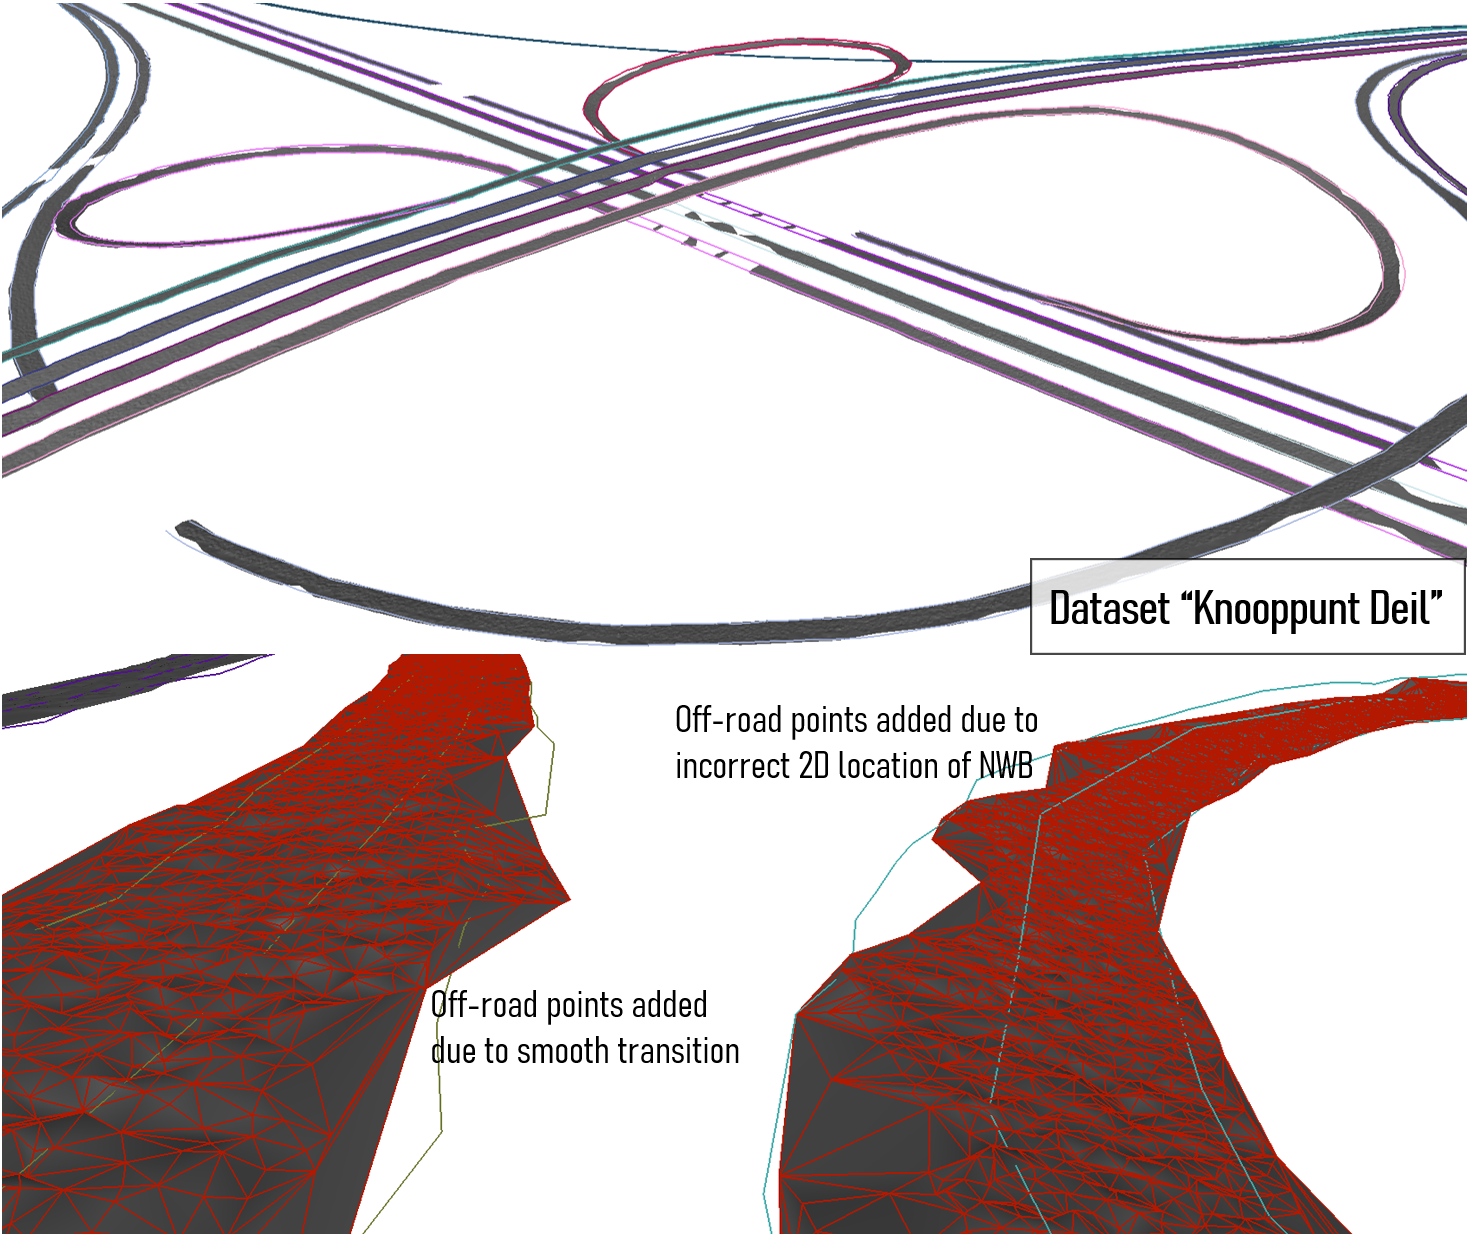
\includegraphics[width=0.9\linewidth]{final_report/figs/tinconstruction1.png}
    \caption[Overview render of constructed TINs and renders of TIN artefacts]{Visualisations providing an overview of constructed \ac{tin}s (above) and illustrating \ac{tin} artefacts (below). The TIN surfaces are shaded in gray, and the preliminary edge geometries are coloured randomly based on their NBRS IDs. The triangulation of some of the TINs is shown as a red wireframe.}
    \label{fig:tinconstruction1}
\end{figure}

\subsubsection{On using small thresholds}

An obvious solution would then be to use preliminary edges that are close to the roads' centrelines, and to make the parametrisation of both \ac{tin} initialisation and \ac{tin} extension even stricter. However, there is a specific reason why this approach is guaranteed to fail: both parametrisations are already lower than \ac{ahn3}'s vertical accuracy. As \ref{sub:ahn} mentions, \ac{ahn3} has an elevation uncertainty of 15 centimetres at 95\% uncertainty. This means that many insertions will actually fail due to the noise, not because of real-life features.

The parametrisation of \ac{tin} initialisation (10 centimetres for elevation/distance tests, 7 degrees for the angles) is already on a scale that falls within the territory of random noise. However, since the radial buffer-filling queries fetch many points rather than just a single neighbour, this generally does not affect the effectiveness of the method; the algorithm will inspect enough neighbours to still find at least a few that are conformant, despite the noise. Even where this fails to an extent, the \ac{tin} extension algorithm will provide the additional passes that are necessary to overcome the issue; this is precisely what happened with the highlighted road in Figure \ref{fig:tinconstruction0}.

As a result of this phenomenon, reducing the thresholds any further without increasing the query radius will inevitably block the surface from spreading into certain areas. Increasing the query radius is, in turn, not desired because it will create too large buffers (increasing computational complexity drastically), and cause large triangles to be constructed in the \ac{tin}, which can in turn act as blocking factors in their own right, if they do not represent the trend of the points in their interior accurately. Using large query radii also increases the chances of spreading the \ac{tin} off the road surfaces, as it will result in more off-road points getting added to the buffers.

In \ac{tin} extension, I could use smaller thresholds than during initialisation because of the differences in the underlying workflow. Since extension considers "layers" of points progressing away from the centres of the road, it considers candidate points in a more "orderly" fashion. In \ac{tin} initialisation, the \ac{tin} only grows towards a certain area if insertions lead the algorithm there, whereas the repeated seeding mechanism in the extension stage represents a more \textit{targeted} growing approach. In practice, this means that the candidates are simply examined in a better order, leading to more efficient decision-making. This counteracts the increased impact the Lidar noise has on the scale of the thresholds that are being used.

A side-effect of this is that growing may be restarted during extension after a relatively large hiatus, leading to large triangles appearing in the \ac{tin}s. The gaps - or more precisely, the small number of successful insertions in them - are mostly caused by the larger, slightly inaccurate triangles which I already mentioned in the previous paragraph. This can be seen in the \ac{tin} structure in the top image in Figure \ref{fig:tinconstruction0} - while the right half of the suspected area of the road has points spaced uniformly, the left side has large, slightly inaccurate triangles that prevented Lidar points from being inserted within their areas and growing the \ac{tin} further in that direction. As the bottom image in the same figure shows, the "second pass" over the data via the \ac{tin} extension solved this issue for the most part, although some of the large triangles remained.

Inspecting a larger area around the point that is being considered for insertion (instead of just the one triangle containing it) could reduce the impact of this issue, but it is costly in terms of computational complexity. This is part of the reason why I only use that approach when inserting points in triangles touching the insertion boundary.

\subsubsection{Note on figures}

Both figures in this section (\ref{fig:tinconstruction0} and \ref{fig:tinconstruction1}) show \ac{tin} road surfaces that appear to be constrained by "invisible" external line geometries, as one would expect large triangles to fill the rest of the convex hull of the vertices in the Delaunay triangulation. Originally, I planned to use a \ac{cdt} to achieve this appearance, but in my final implementation I merely improved the appearance of the models before visualising them by removing meaningless triangles based on area and circumference thresholds. This proved to be effective in eliminating the large triangles and sliver triangles that appear in the \ac{dt} to fill the convex hull of the inserted points.

While these redundant triangles represent no issue in terms of interpolating elevations for \ac{nwb}, they make the visual interpretation of the results difficult. Exporting the \ac{tin}s after generating them automatically applies this filtering step in the final release of my code.

In this context, it is also important to point out that while \ac{ahn3} data gaps that are patched in with \ac{dtb} data are always completely covered by triangles in the \ac{tin}s if the preliminary edges extend through the gap. The reason why in the top image in Figure \ref{fig:tinconstruction1} this appears not to be the case, is that some of these triangles were large enough to be filtered out to improve visual appearance. The thresholds can be adjusted in my code to alter this behaviour.

\subsubsection{TIN point density}

While using 50\% of the \ac{ahn3} point density (via a thinning factor of 2) offered practical benefits for all pipeline steps up to this point (especially the Lidar segmentation and edge approximation steps), the \textit{quality} of the generated \ac{tin}s does not significantly increase as a factor of point density.

Before running the \ac{tin} construction procedure, the program is equipped with subclouds, each with Lidar points relevant to a specific \ac{nbrs} part. Since all prior steps are configured to keep as many of the surface points as possible, it is generally the case that their point density on the road surface is comparable to the thinned point density of the imported \ac{ahn3} data. Inserting such a large volume of points into the \ac{tin} may not always be practical. For instance, visualising the generated surfaces becomes slow even with modern software, and the stochastic Lidar noise becomes clearly visible (the ripples can be seen very clearly in Figures \ref{fig:tinconstruction0} \ref{fig:tinconstruction1} due to the 5-fold vertical exaggeration). This much detail may also be impractical for applications that deal with modelling processes on the surface itself, and has implications for the accuracy assessment (see Section \ref{sec:accuracy}).

The performance of this step thus depends on the input Lidar thinning. In practice, a thinning factor of 2 means that we are still working with around 10-30 Lidar points per m\textsuperscript{2}, which results in mediocre performance. While my implementation did take performance considerations into account initially (for instance the buffer-filling approach is the result of this), later modifications, such as working with multiple triangles and plane fitting when growing the road surface, resulted in the performance of the final implementation decreasing gradually. In particular, not running \ac{tin} extension can improve runtimes drastically, which may be useful for users who are only interested in interpolating \ac{nwb} elevations.

As I will further explain in Section \ref{sec:accuracy}), the system design guarantees that \ac{nwb} will generally lie on the \ac{tin} models in 2D, making it possible to interpolate elevations in it for its vertices. Exceptions to this rule occur in places where preliminary edge estimates or optimised edges disagree with \ac{nwb} badly. Where this occurs, \ac{tin} initialisation will not be able to insert points in the \ac{tin}s at the 2D location of \ac{nwb}. With preliminary edges, this may only occur where cross-sections were skipped too many times in a row where the road is not straight, which may happen in various circumstances I have already described in Section \ref{sub:r_edgeapproximation}. With active contour optimisation, this may occur more frequently, depending on the local density of generated artefacts.

\subsubsection{Two different kinds of quality}

While the above discussion focuses on describing issues with the quality of the generated \ac{tin}s, many of these issues are constrained to the academic goals of the project only. The academic goal related to the \ac{tin}s is to make them complete and accurate representations of the real-life road surfaces. This is the quality on which I primarily focused in this section, while the next section will see more mentions of quality in terms of their suitability for interpolating elevations for \ac{nwb}.

These two qualities need to be distinguished not only because of the conceptual differences, but because there are much less issues with the less academic goal of converting \ac{nwb} to 3D than with producing ideal road surface models. The reason is, that for the 3D conversion to be accurate, one only needs complete and accurate \ac{tin} surfaces close to where the centrelines are found in 2D. Fortunately, these locations generally correspond to areas which are less difficult to reconstruct accurately in 3D, than for instance the immediate vicinity of road edges.

\subsubsection{Using the implementation}

The following two commands may be used to run \ac{tin} construction and export the resulting 3D surface models:

\begin{verbatim}
roads.build_tin(max_dh_int = 0.1, max_angle_int = 0.12, r_int = 1,
                max_dh_ext = 0.03, max_angle_ext = 0.04, r_ext = 0.8,
                ext_steps = 5, ext_dist = 0.5,
                type_edges = 'preliminary')
roads.write_tins(fpath = tin_fpath)
\end{verbatim}

The first method invocation performs the \ac{tin} construction itself. The first line of arguments corresponds to the elevation and angle thresholds, and the buffer-filling query radius used in \ac{tin} initialisation, respectively. The role of the second line of arguments is identical, with the exception that they are used for \ac{tin} extension. The next two arguments (\codeword{ext_steps} and \codeword{ext_dist}) specify the number of extension steps to be performed, and the distance by which the query region should be expanded in each step. The first insertion boundary for extension is always a polygon created by buffering the seed LineString by 0.5 metres; the extension starts from this base boundary. If no extension is desired, \codeword{ext_steps} should be set to 0. The last parameter, \codeword{type_edges} can be set either to \codeword{preliminary} or \codeword{optimised}; it controls which type of road edges the user desires to use.

The second method invocation writes the \ac{tin}s to disk, one OBJ file for each \ac{nbrs} part As mentioned above, it also filters out large triangles and sliver triangles in the process. The supplied file path should only include the first part of the file name, as the \ac{nbrs} ID, part ID and file extension will be added automatically (for instance \codeword{.../C_39CZ1_tin} would work. Using a dedicated folder is recommended.

\subsection{Interpolation in TIN and snapping}
\label{sub:r_interpolation}

\begin{figure}
    \centering
    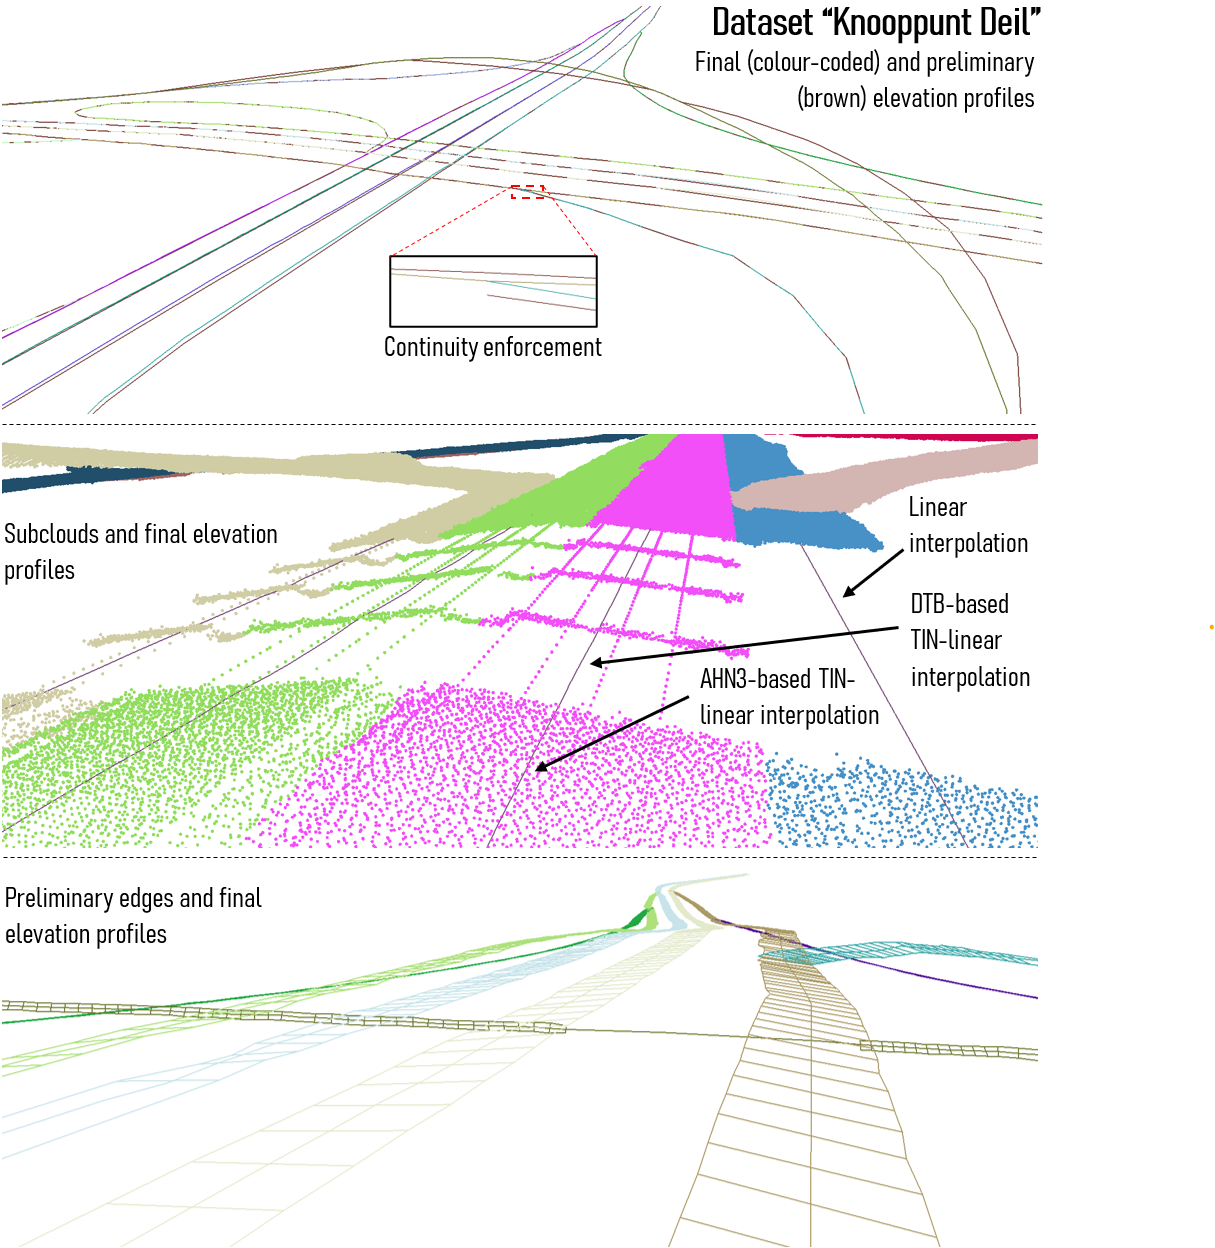
\includegraphics[width=\linewidth]{final_report/figs/elevationinterpolation0.png}
    \caption[Visualisations comparing final 3D-NWB geometries with intermediate results]{Visualisations comparing final 3D conversion results to preliminary conversion (above), subclouds (in the middle), and preliminary edges (below). In the upper visualisation, the final 3D-NWB geometries are shown coloured randomly based on their NBRS IDs, and the preliminary 3D conversion in brown. In the subcloud comparison, the subclouds are also coloured based on their NBRS IDs, and here the final 3D conversion of NWB is shown in a constant colour to help distinguish it from the points. In the bottom visualisation, the final 3D-NWB geometry, as well as the preliminary edges and cross-sections are coloured randomly, based on their NBRS IDs.}
    \label{fig:elevationinterpolation0}
\end{figure}

Figures \ref{fig:elevationinterpolation0} and \ref{fig:elevationinterpolation1} show examples of the results of interpolating elevations for \ac{nwb} in the \ac{tin}s generated in the previous step (including the use of the snapping feature that enforces continuity)). Visual inspection of the results reveals that the methods used to generate them are robust and effective under almost all circumstances, including where complex 3D relationships and the extensive presence of other types of occlusion are encountered. The example visualisations shown here contain comparisons between the final elevation profiles and various intermediate results, namely the preliminary elevations, subclouds and preliminary edges in Figure \ref{fig:elevationinterpolation0}, and the \ac{tin} models in Figure \ref{fig:elevationinterpolation1}).

Generally, the results are in line with my expectations both in terms of overall completeness and quality. I do not attempt to characterise the accuracy of the results in this section, for a quantitative (rather than qualitative) analysis, please refer to \ref{sec:accuracy}.

\subsubsection{Comparison with preliminary elevations}

Comparing the final 3D-NWB results with the preliminary elevations sheds some light on the nature of the improvements that are the result of the complex processing steps that occur in the later stages of the pipeline. The preliminary elevations (shown in a brown colour in the top visualisation Figure \ref{fig:elevationinterpolation0}) represent the 3D conversion that can be achieved using only a few simple steps of processing: \ac{nbrs} generation, elevation estimation, and the polynomial-based refinement step. The final results are coloured randomly based on their \ac{nbrs} IDs.

The first difference that stands out is that those \ac{nbrs} that I described as having complex vertical curvature and being difficult to model by polynomials in Section \ref{sub:r_elevationestimation} are modelled much more realistically in the final output. One only needs to take a look at the comparison in the top image in Figure \ref{fig:elevationinterpolation0}) to tell that it must be the final results that are correct, not the preliminary ones. The change represents a fundamental difference between these two stages in the pipeline. Preliminary elevation estimation has to rely on a workflow to detect elevation estimates corrupted by occluding geometry and to supply replacement values for them, while the final elevations come from \ac{tin} models that are guaranteed to only contain vertices that represent measurements of the relevant road's elevation.

While the biggest differences can be observed where the polynomial fits were poor in the preliminary elevation estimation stage, there are many other scenarios where smaller improvements can be seen. For instance, the preliminary elevations may contain outliers that were not detected as outliers in the refinement step. For instance on bridges, \ac{ahn3} may contain reflections from vehicles. These are often not far enough from the road surface to be replaced by polynomial values, introducting small spikes into the elevation series. In the final results, such outlier points are guaranteed not be be inserted into the \ac{tin} models, and cannot affect the 3D conversion as a result. The inset in the figure also illustrates that while while preliminary 3D conversion is not continuous across intersections, the snapping workflow ensures that the final 3D conversion is.

Another scenario in which clear benefits can be observed (not shown on these figures) is the presence of many occluded regions concentrated into a small area, or equivalently, one long occluded zone. In preliminary elevation estimation, such occluding features may attract the polynomial towards themselves, thus corrupting the fit and potentially introducing incorrect elevations into the profiles. This may happen, for instance, where many bridges are constructed across a motorway in a row, and the \ac{nbrs} is not long enough to include enough non-occluded elevation measurements. Later pipeline steps almost always recognise these mistakes for what they are (data gaps), and either use \ac{dtb} if available, or break the \ac{nbrs} into parts locally.

There are features in the final output that may be interpreted as a deterioration in quality with respect to the preliminary elevations, at least visually. Firstly, small jumps in elevation may be observed where \ac{ahn3} gives way to \ac{dtb} points the underlying \ac{tin}s. The new baseline elevation continues across the region where \ac{dtb} was used, and reverts to the \ac{ahn3}-based baseline elevation once the road emerges from the zone not covered by \ac{ahn3}. This is simply due to the temporal discrepancy between \ac{dtb} and \ac{ahn3}; using better support data would eliminate these shifts from the output. This is only visible in the middle image in Figure \ref{fig:elevationinterpolation0}, and the reader is referred to Figure \ref{fig:lidarsegmentation1} and Sections \ref{sec:accuracy} and \ref{sec:r_comparison} for further details.

Lastly, one may observe that the amount of small-scale noise in the final 3D-NWB output is noticeably larger than that in the preliminary profiles. This also has a simple explanation: the preliminary elevations are based on taking the median of the elevations of a small patch of Lidar points, whereas the final elevations are all based on 3 samples each, due to having used TIN-linear interpolation. The amount of noise is thus no greater than the stochastic scatter in \ac{ahn3}; it is only visible in the visualisation due to the vertical exaggeration. This scatter is unimportant in terms of the noise modelling application.

\subsubsection{Comparison with subclouds}

This comparison is demonstrated in the middle image in Figure \ref{fig:elevationinterpolation0}. The most important aspect here is that the final 3D road centrelines all lie flat on those parts of the Lidar subclouds, which one intuitively recognises as road surfaces. This is always the case as long as \ac{nwb} is correctly positioned, such as in this location.

The figure shows that this also holds for regions affected by occlusion. In places where \ac{dtb} was added to the subcloud in the Lidar segmentation step, the centrelines are shifted vertically to conform with the surfaces defined by \ac{dtb}. Where \ac{ahn3} coverage reappears, they immediately shift back to its elevation, creating a geometry akin to suspension bridges in this example visualisation. Regardless of which dataset is used, the main point here is that the 3D conversion continues across the gaps without snapping to the bridges above that are causing the periodic occlusion.

The visualisation also illustrates that linear interpolation through regions with no measurements represents a good solution for small gaps of coverage where roads are straight. The road with the blue-coloured subcloud (on the right) has no \ac{dtb} coverage, hence the small patches of \ac{ahn3} points between the bridges could also not be detected. In spite of this, the elevations are actually more optimal here than elsewhere, because they are not affected by the small sifts introduced by \ac{dtb}.

\subsubsection{Comparison with preliminary edges}

This comparison reveals the interestingly, the final 3D conversion of the centrelines and the preliminary edges are in near-perfect agreement with each other where coverage is good. As the bottom image in Figure \ref{fig:elevationinterpolation0} shows, even a five-fold vertical exaggeration cannot reveal significant differences between them. This is interesting, as there are various pipeline steps in-between the generation of these results; most importantly, \ac{tin} generation. Small differences are only found between the elevations of the preliminary edges and 3D-NWB, where the preliminary edges were generated off the road surface, in which case the final results represent the correct elevation.

While the two outputs are not directly comparable, the exceptionally good match between them indicates that a 3D conversion with similar quality could potentially be achieved via a procedure that involves the subclouds and 2D centrelines only, perhaps using a workflow based to some extent on that which currently I used to generate the preliminary edges.

It is also important to note here that while the preliminary edges may be missing vertices in some places (indicated by the cross-sections also being absent), this is not the case in any of my final 3D-NWB results. As long as the centreline is found between the edges, a \ac{tin} will be constructed locally and TIN-based elevations will be computed. As I already described previously, this is only violated in places where many cross-sections are skipped in a row, which is rare in my results.

\begin{figure}[h]
    \centering
    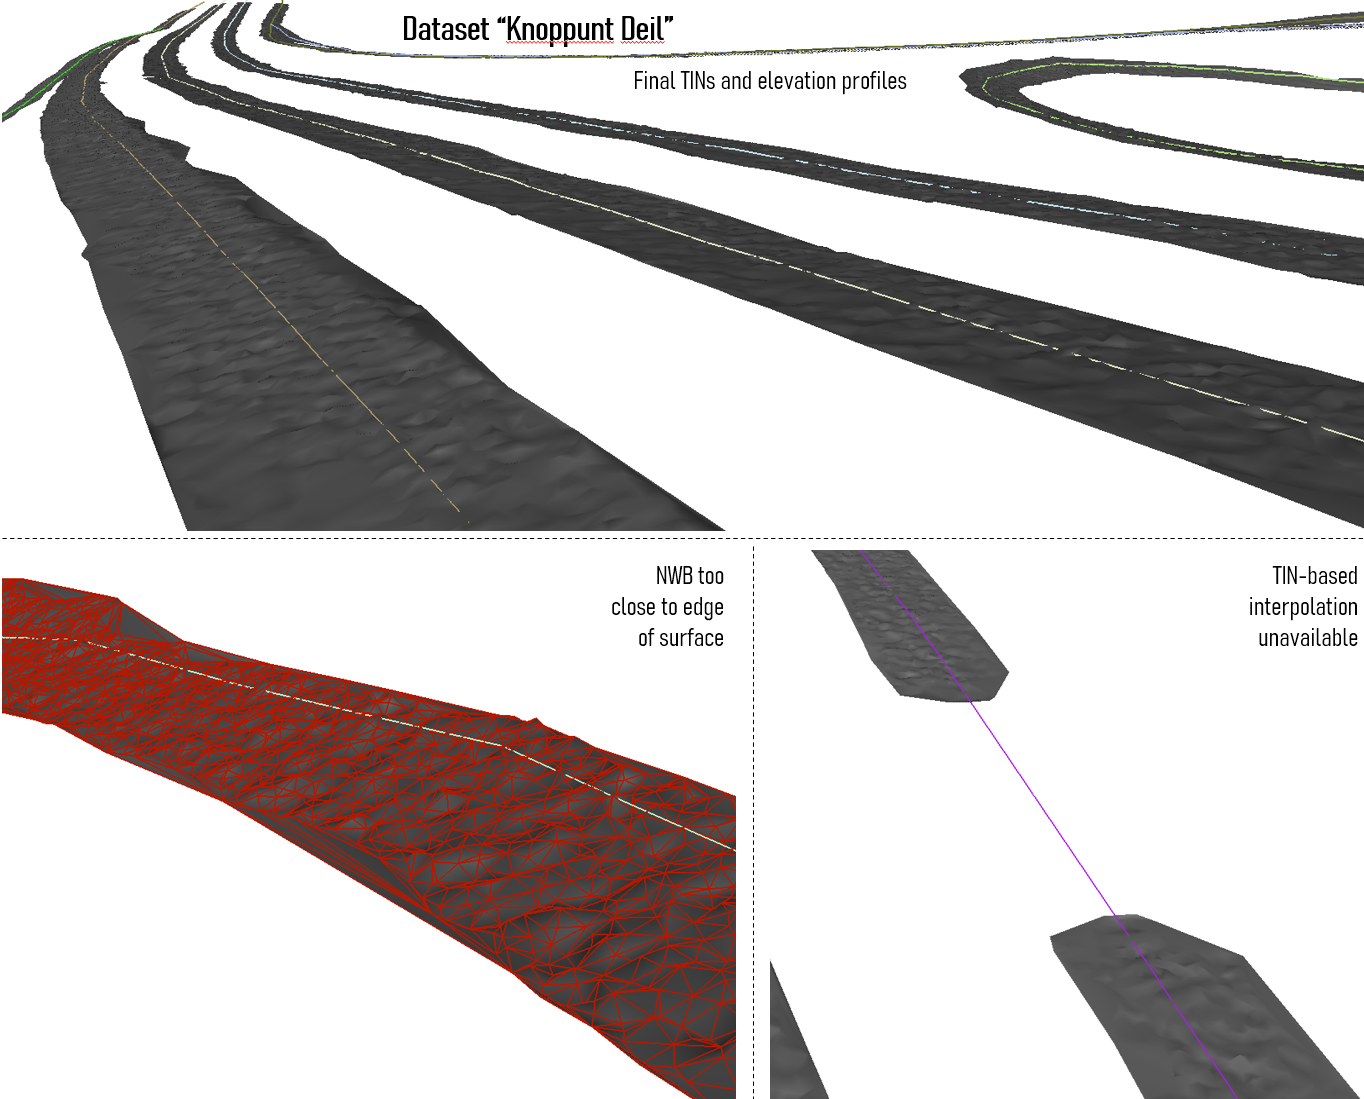
\includegraphics[width=0.9\linewidth]{final_report/figs/elevationinterpolation1.png}
    \caption[Renders comparing final 3D-NWB geometries with the underlying TIN models]{Visualisations comparing final 3D conversion results to the underlying \ac{tin} models. The TIN surfaces are shaded in gray, and the final 3D-NWB geometries are coloured randomly based on their NBRS IDs. The triangulation of one of the TINs is shown as a red wireframe.}
    \label{fig:elevationinterpolation1}
\end{figure}

\subsubsection{Comparison with TIN models}

Example comparisons between the final output and the \ac{tin}s are shown in Figure \ref{fig:elevationinterpolation1}. An interesting aspect of this comparison is that the final 3D-converted centrelines are often found slightly above or below the model (less than a centimetre, typically). This is best evidenced in the output by the intermittent disappearance of the 3D centrelines beneath the \ac{tin} triangles. This is the result of the georeferencing of \ac{nwb} being coarse \textit{relative to the \ac{tin}s} even after applying vertex densification. \ac{nbrs} parts only have vertices approximately every 5 metres, whereas \ac{ahn3} has up to 10 to 30 points per m\textsuperscript{2} after after thinning using a factor of 2.

This disparity simply indicates that if we wanted to, we could sample the \ac{tin} at smaller intervals to increase the output's vertical resolution. This would allow steep road segments to be better characterised in the output. In the case of flat road surfaces, no improvement would be noticeable. \ac{ndw} officially requires elevations to only be estimated at the \textit{original} \ac{nwb} vertices, which can be many times further apart than my densified vertices. In other words, these \ac{tin}s offer far more detail than that which would be minimally required for the conversion, as expected from such a high-resolution surface model. However, using only the original vertices loses so much vertical detail that I recommend retaining the densified vertices, even if this means that a stark contrast will be present between the horizontal and vertical resolution of the output.

An example where \ac{nwb} gets close to the edge of the \ac{tin} is shown in the bottom left image. This is representative of the typical severity of the \ac{nwb} georeferencing issue in sharp bends. While it was difficult to overcome numerous processing difficulties related to this problem with \ac{nwb}, it bears almost no influence on the \textit{effectiveness} of the \ac{tin} interpolation process as long as the \ac{tin} exists locally. Where \ac{nwb} lines are close to road edges, the underlying \ac{tin} models will still always describe the surface of the road according to our expectations. They will potentially include off-road points, but from the point of view of the 3D conversion of \ac{nwb}, this does not matter. Even if \ac{nwb} is not on the road surface, the \ac{tin} will likely be constructed locally and off-road elevations will be interpolated for it - although this means that the resulting elevation series will be corrupted locally. The elevation of the surrounding terrain will be reflected in it instead of that of the road.

The interpolated elevations will always correspond to the exact horizontal position of \ac{nwb}, meaning that as long as its georeferencing is not corrected, the interpolated elevations will also not always correspond to the road's real centreline. As I noted above, this could cause problems if \ac{nwb} is not on the road surface. However, even if it \textit{is} on the road surface, a small overestimation or underestimation relative to the elevation of the centre of the road is possible, if the road's surface has a significant sideways tilt. Rectifying \ac{nwb}'s georeferencing would automatically solve these issues and would also improve the effectiveness of many previous steps. No modifications to the algorithms would be needed to achieve this.

Where no \ac{ahn3} \textit{or} \ac{dtb} coverage is available, the \ac{tin} will not exist and values are interpolated linearly inside the elevation profiles. A location with this property is shown on the bottom right in Figure \ref{fig:elevationinterpolation1}. Such gaps correspond to zones \textit{between} \ac{nbrs} parts, hence the two \ac{tin}s shown in this image belong to two different \ac{nbrs} parts.

\subsubsection{Using the implementation}

The following two commands may be used to run the final elevation interpolation code, and export the resulting 3D-converted version of \ac{nwb} as a Shapefile:

\begin{verbatim}
roads.interpolate_elevations()
roads.write_all(fpath = accurateZ_fpath,
                to_drop = ['geometry_simpleZ'])
\end{verbatim}

The algorithm does not have a parametrisation, hence the method invocation does not require any arguments. The \codeword{.write_all()} invocation requires a list of GeoDataFrame columns to drop, as the Shapefile can only have one set of geometries in it. The column name in \codeword{['geometry_simpleZ']} corresponds to the preliminary elevation estimates. The original 2D \ac{nwb} geometries are always dropped automatically, so that column does not need to be manually specified.

In the \codeword{nbrs_manager} class, the final results are added to the class's \codeword{.nwb} variable, as the \codeword{geometry_simpleZ} geometry column of the GeoDataFrame. Since Shapefiles also cannot accept arrays into their attribute tables, the vertex origin indicators (AHN3/DTB/linear interpolation) are also not written into the output file. These can be found in \codeword{.wvk_z_origins[wvk_id]}, a dictionary that needs to be indexed with the \textit{wegvak}'s ID whose vertex origins are desired.

\section{Accuracy assessment}
\label{sec:accuracy}

In this section, I will present the accuracy assessment results focusing on a particular dataset: \textit{Knooppunt Deil}. This dataset exhibits most of the unique features that are relevant for this part of the analysis, and it is my hope that such a "case study" approach makes understanding the assessment's results more straightforward. Following the case study, I will present and discuss an overview of the relevant accuracy metrics for all testing datasets, in a tabulated format.

I will first focus on the results of computing local sampling densities and formal output accuracy values (error propagation results). Then, I will discuss how often the accuracy needs to be deemed unknown and for what reasons. Lastly, the completeness of the output \ac{tin}s relative to the \ac{bgt} reference polygons will be examined. Please refer to the relevant sections in Chapter \ref{chap:mm} (\ref{sub:accuracyoverview} and \ref{sec:m_accuracyassessment}) for the background theory and the detailed description regarding the assumptions I made.

\subsection{Empirical accuracy assessment}
\label{sub:accuracyempirical}

\begin{figure}
    \centering
    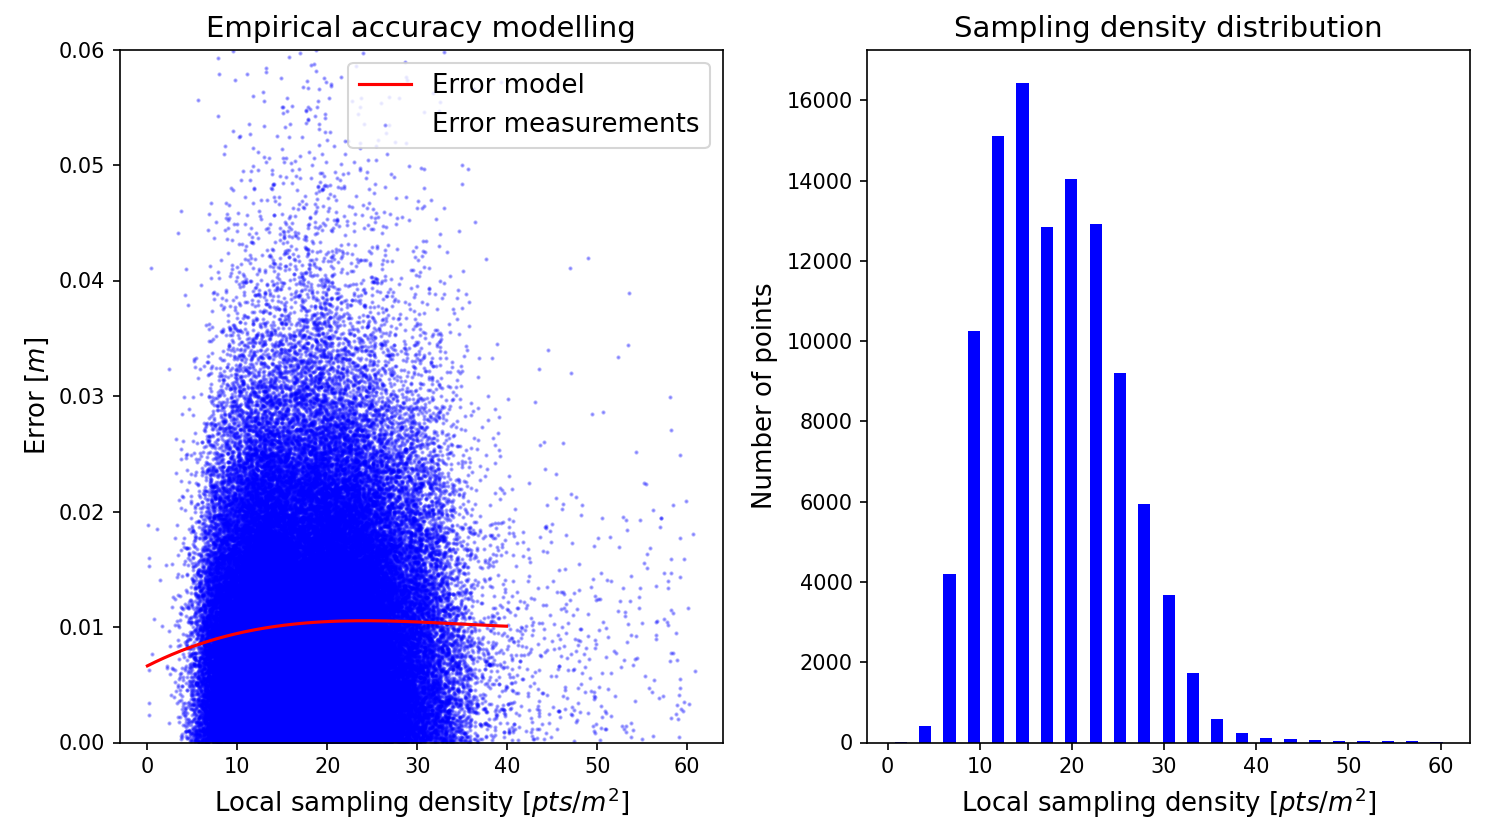
\includegraphics[width=\linewidth]{final_report/figs/empiricalaccuracy0.png}
    \caption[Charts demonstrating the outcome of the empirical accuracy assessment process]{Charts demonstrating the outcome of the empirical accuracy assessment process.}
    \label{fig:empiricalaccuracy0}
\end{figure}

As I briefly mentioned in Section \ref{sub:accuracyoverview}, I first attempted to assess accuracy based on an empirical approach. Before performing the necessary steps, I was yet unaware of how the combination of factors that define output accuracy interact in our particular case. Most importantly, I was yet to discover that a range of assumptions regarding ground filtering accuracy, influence of surface ruggedness and sampling density can be made. In fact, it was this failed attempt that directed my attention to the fact that in our particular case, there are very few external factors that influence accuracy.

My initial hypothesis was that the primary influence on accuracy has to be sampling density and interpolation error, because ground filtering errors and surface ruggedness already appeared to me as irrelevant based on my experience with the data and the results. To be able to verify the hypothesis and compute empirical errors based on it, I constructed an error model and derived errors for each output vertex from it. I constructed the model by removing samples (vertices) from the output \ac{tin}s, interpolating their values via the TIN-linear method, and computing the differences between the removed Lidar samples, and the interpolated elevations (in essence, a jackknife approach). I fit a cubic polynomial on the part of the scatter where we have enough data, and derived \ac{nwb} accuracy values from it.

While I was doing this, I noticed that all my output errors were extremely small, and all roughly the same. This made me start suspecting the irrelevance of sampling density in our particular scenario, so I plotted the data and the model to verify this new hypothesis. Figure \ref{fig:empiricalaccuracy0} shows an example visualisation created from the empirical accuracy assessment of testing dataset \textit{Knooppunt Deil}. The chart on the left shows local sampling density plotted against the jackknife errors, computed for about 10\textsuperscript{5} \ac{tin} vertices (10\% of the total number of \ac{tin} vertices of all \ac{tin} models generated from this testing dataset).

While at a first glance one might think that the inverse parabola shape in the scatter plot represents a meaningful trend, it does not, in fact, possess the correct shape for the relationship. We know from literature that when a correlation exists between errors and sampling densities, it tends to be logarithmic, and the trend in my chart does not appear to have that property. The fitted model does appear to have a weak logarithmic component, but it shows errors to increase in the wrong direction (towards larger sampling density), and the predicted error magnitudes are far too small to be meaningful too. The histogram on the right reveals that the shape of the scatter plot does not correspond to a statistical trend that concerns a relationship between sampling density and jackknife error - it can be fully explained by the distribution of the sampling densities in the dataset.

What is also interesting in these plots, is that jackknife errors remain negligible even at the lowest values encountered. Overall, about 96\% of the jackknife samples showed an error less than 3 cm, which is well below the nominal vertical and horizontal accuracies of \ac{ahn3} and \ac{dtb}. In other words, we may safely conclude that the variation in jackknife accuracy, on the scale observed in this experiment can be explained simply by the noise in the input datasets. The random distribution of the variations, evidenced by the bell-shaped trend, further confirms this theory.

Although this analysis suggests that any errors in the output will be small and that they will be mostly independent of external factors, the qualitative and quantitative estimation of output accuracy is among the main goals of this project, hence I decided to find further evidence. This is why, even after performing the above analysis, I proceeded to propagate errors through the interpolation technique, and to also examine this in comparison with sampling density data.

\subsection{Formal accuracy assessment}
\label{sub:accuracyformal}

\begin{figure}
    \centering
    \includegraphics[width=0.9\linewidth]{final_report/figs/formalaccuracy0.pdf}
    \caption[Charts illustrating the formal accuracy assessment results on two LineStrings]{Charts illustrating the formal accuracy assessment results on two \textit{wegvakken}.}
    \label{fig:formalaccuracy0}
\end{figure}

\begin{figure}
    \centering
    \includegraphics[width=0.9\linewidth]{final_report/figs/formalaccuracy1.png}
    \caption[Renders showing the subclouds, TINs and 3D-NWB centrelines relevant to Figure \ref{fig:formalaccuracy0}]{Visualisations showing the subclouds, \ac{tin}s and 3D-NWB centrelines in the area concerned by Figure \ref{fig:formalaccuracy0}. In the top visualisation, the subclouds and final 3D-NWB geometries are shown coloured randomly based on their NBRS IDs. In the bottom visualisation, the TIN surfaces are shaded in gray, and the final 3D-NWB geometries are coloured randomly based on their NBRS IDs.}
    \label{fig:formalaccuracy1}
\end{figure}

The charts in Figure \ref{fig:formalaccuracy0} show interpolation error profiles from 2 \textit{wegvakken} from our chosen testing dataset. From the lack of a trend in the errors, and their small magnitudes overall, we may deduce that the output accuracy is sufficiently high with respect to the 20-centimetre requirement of the noise regulations. Any differences due to the TIN-linear interpolation represent an \textit{increase} in accuracy relative to the 15 cm elevation accuracy of \ac{ahn3}. The two \textit{wegvakken} shown in the figure exhibit theoretical interpolation elevation errors in a range of about 4 centimetres to 7 centimetres, with mean errors of 5 centimetres for both. The variation is always randomly distributed, because the positions of \ac{nwb} vertices relative to the containing triangles' vertices also lack correlation (which is what controls the value $M$ that determines how much the accuracy is improved). In theory, the only factor that could introduce correlation into these profiles would be roads with very steeply sloping surfaces, but no roads in this dataset (or any of my datasets) reach a slope steep enough to affect the errors significantly, and introduce correlation.

The top part of Figure \ref{fig:formalaccuracy1} shows the 3D geometry of the subclouds and centrelines of the same two \textit{wegvakken}. \textit{Wegvak} \#288259033 has a shape which is representative of the steepest slopes and sharpest bends one can expect from the Dutch road network; it connects a ground-level motorway lane with another one running orthogonal to it directly above, on a bridge. \textit{Wegvak} \#600127973 is the ground-based motorway lane that it connects. It lies entirely flat on the ground, with little to no variation in its elevation. I picked it because its shape is the opposite of that of \#288259033, and because it had been split into two parts due to a 15-20 m long data gap which is visible in the figure. The gap also lacks \ac{dtb} coverage. The bottom image in Figure \ref{fig:formalaccuracy1} shows the corresponding \ac{tin}s, and it is visible in this figure that \ac{nwb} veers to the outer edge of the steep, curved \textit{wegvak}, almost reaching it. The relatively thin width of the \ac{tin} and its rugged outer edge is a result of this; the preliminary edges were constructed partially off-road due to \ac{nwb}'s poor georeferencing.

I added sampling density plots on the right in Figure \ref{fig:formalaccuracy0}. The first important observation to make about these charts is that the data gap in sampling density between 100 and 200 m along the profile in \#600127973 is due to the data gap I mentioned above; here the density is 3 points per m\textsuperscript{2} or less - which is the threshold below which the cut-out happens, i.e. accuracy is not computed - visible in the chart on the left in the same figure. The sharp drops in density around the gap illustrate that the neighbourhood queries already indicate the presence of the gap right before and after reaching the centreline vertices that fall into it. The two \textit{wegvakken} \#288259033 and \#600127973 have mean sampling densities of 24 and 21 points per m\textsuperscript{2} respectively - well above the nominal accuracy of the dataset, primarily owing to the flatness of the road surfaces.

The second important observation is that while local sampling density fluctuates by as much as 80-90\%, it never reaches the minimum threshold in places other than no-data zones and where only \ac{dtb} data is available (the latter is not separately illustrated here). The fluctuation is due to the inhomogeneous sampling rate of \ac{ahn3}. It is already present in the raw point cloud, and is simply a factor of how many times a given area was scanned by the aircraft's laser sensors. The figure was generated from my final results, which all use a thinning factor of 2 - meaning that the values seen in the charts are half of the maximum available. Increasing the thinning factor further may result in the sampling rate dropping below the threshold in certain exposed regions, hence it is not recommended. The results shown in these two charts are representative of all testing tiles; significant deviations from what I described above and what is shown in the figure were not observed elsewhere either.

The third, and last important observation is that neither the recorded sampling rates, nor the theoretical accuracy values are indicative of locations where \ac{nwb}'s 2D georeferencing is poor. While \ac{nwb}'s location is far from the road's real centre in \#288259033, it is not off the road, and as a result the interpolated elevations will still be correct, or at least they will definitely correspond to some part of the road surface. As far as theory is concerned, the elevation is the \textit{correct elevation} at the \textit{incorrect \ac{nwb} location}. This also holds for places where \ac{nwb} is not on the road surface, but in such places both the sampling density and the accuracy may drop, the former because the \ac{tin} construction algorithm is not meant to be used in uneven areas, and the latter because of (and only in the case of) introducing sloping triangles into the \ac{tin}.

The mean error and sampling density of the entire testing dataset are 5 cm and 19 points per m\textsuperscript{2} respectively.

\subsection{Ratio of accurate vertices}
\label{sub:completeness}

The frequency at which the algorithm has to deem output accuracy unknown fluctuates significantly both inside and between testing datasets. How often this happens depends on the number of linearly interpolated values, and how often the sampling density drops below the 3 points per m\textsuperscript{2} threshold. The percentage ratio of accurate vertices varies, under normal circumstances, between 85 and 95\%. Special circumstances (such as tunnels) may further decrease this, which will be discussed in Section \ref{sub:accuracytabulated}.

Where no special circumstances are encountered, variations can be traced back to two main controlling factors: how much of the road network is occluded, how accurate the preliminary elevations are, and how complete \ac{dtb} is in the given testing dataset. The relevance of the amount of occlusion is straightforward to understand: the more the occlusion, the bigger the chances are of encountering an \ac{ahn3} data gap where linear interpolation may need to be used.

The completeness of \ac{dtb} is a factor here because it prevents linear interpolation from being used. However, for the program to consider interpolation accurate locally, \ac{dtb} \textit{also} needs to have good enough coverage. Therefore, only a subset of the \ac{dtb}-covered data gaps will be deemed accurate. \ac{dtb} rarely exists for provincial roads (\ac{p_roads}), hence Lidar data gaps in such roads will \textit{almost always} result in linear interpolation. In turn, this means that data sets comprised primarily of \ac{p_roads} will have lower accurate vertex ratios. Preliminary elevation accuracy is important, because it controls \ac{dtb} coverage. If the preliminary elevations are inaccurate (due to a poor polynomial fit, in most cases), then even if \ac{dtb} exists locally, it may not be found.

As I mentioned in Section \ref{sub:accuracyoverview}, \ac{dtb} is effectively a placeholder for a more accurate dataset in terms of this accuracy assessment workflow. Records of which vertices were affected by \ac{dtb} data are generated by my implementation, and reusers are advised to consider all of these vertices inaccurate due to the temporal issues. For the purposes of this accuracy assessment demonstration, \ac{dtb}-based interpolation with high enough local sampling density was considered accurate and included in the percentage values. However, because \ac{dtb}-based sampling density also reflects the line densification threshold used when converting it to a point cloud (in addition to the number of \ac{dtb} lines available locally), I must emphasise here that \ac{dtb}-based sampling density values are partly artificial.

Linear interpolation is rare outside of \ac{ahn3} data gaps (including those due to occlusion), and especially rare where \ac{nwb}'s georeferencing is correct - in my datasets, 98-100\% of non-occluded vertices are interpolated in the underlying \ac{tin}s. The majority of these are due to the rare cases where too many cross-sections are skipped during preliminary edge estimation, preventing proper \ac{tin}s from being constructed locally.

\subsection{TIN completeness}
\label{sub:tincompleteness}

\begin{figure}[h]
    \centering
    \includegraphics[width=0.8\linewidth]{final_report/figs/bgtcomparison.png}
    \caption[2D comparison renders of NWB, BGT and aerial imagery]{Above: 2D visualisation comparing \ac{bgt} road edges with the \ac{tin}s (beige lines and beige wireframes). Below: comparison of \ac{bgt} road edges (dark brown) with \ac{nwb} centrelines (bright green) and with Luchtfoto 2020 aerial imagery.}
    \label{fig:bgtcomparison}
\end{figure}

As I mentioned in the methods section, I evaluated the completeness of the \ac{tin} road surface models via a comparison with \ac{bgt} polygons. Figure \ref{fig:bgtcomparison} shows the results of one such comparison, which I deemed representative of the relationship overall. The top part of the figure shows some of the \ac{tin}s overlain on the outlines of \ac{bgt} geometries, which allows one to see how well the \ac{tin}s agree with these reference geometries. The bottom half of the figure, in turn, compares the \ac{bgt} geometries to satellite imagery - to verify how well \ac{bgt} itself agrees with what we can consider an accurate representation of the visual appearance of these roads. The orthoimagery is from the 2020 edition of Kadaster's Luchtfoto dataset, available as open data like all other datasets used in this research.

The \ac{nwb} centrelines are also shown here to demonstrate the extent of the georeferencing issues relative to \ac{bgt} and to the orthoimagery. The poor agreement is the result of two factors combined: \ac{nwb} approximates the centre of the traffic-occupied road surfaces rather than the paved surfaces, and its georeferencing is inaccurate in general. The definition of traffic-occupied road surfaces excludes hard shoulders. If the traffic-occupied surface is on one edge of the full paved surface, \ac{nwb}'s poor georeferencing is more likely to cause it to be close to, or beyond the real edge of the paved surface.

\ac{bgt}, on the other hand, appears to be an accurate 2D representation of the paved road surfaces. Its extents do not, however, correspond to that which I can \textit{typically} model reliably using the pipeline I developed. Ideally, the surface model should cover the entire paved area, but as I described in Section \ref{sub:m_edgeapproximation}, I found using a maximum road width to be the only viable means to ensure that my approach works in most cases. The \ac{tin} extensions that are part of the \ac{tin} construction step (Section \ref{sub:m_tinconstruction}) mitigate this issue to a certain extent, but they do not eliminate it entirely. Allowing the \ac{tin} extension to go too far beyond the preliminary/optimised edges increases the chances of extending the roads into unwanted areas, and increases runtimes significantly.

Motorways with hard shoulders, which are shown in the centre of Figure \ref{fig:bgtcomparison}, are particularly difficult to handle because the hard shoulders and potential extra lanes extend their width far beyond that, which could be reasonably expected from municipal roads and dual carriageways - which is what my parametrisation prioritises. A solution to this issue could be to automatically select pre-set configurations of the parametrisation appropriate to each road type, but this is not an area that my research explored.

The \ac{tin} models in the top part of the figure show that the \ac{tin}s are in good agreement with the \ac{bgt} geometries. The same issues which I described in Section \ref{sub:r_tinconstruction} are also manifested here, for instance the on-ramp model in the top of the image contains some off-road points where both \ac{nwb} and \ac{bgt} appear to veer too far from their ideal positions. In general, based on examining all my results, I estimated that the \ac{tin} surfaces cover approximately 95\% of the traffic-occupied surfaces found in my testing datasets, and about 75\% of the total paved surfaces as shown by \ac{bgt}. The only major issue appears to be the one I mentioned above, that the full extent of the paved surfaces cannot be modelled without dynamically adjusting the parametrisation of the pipeline's algorithms.

Figure \ref{fig:bgtcomparison} is also illustrative in terms of showing just how detailed these \ac{tin} models are, even with an input thinning factor of 2 for \ac{ahn3}. On the scale shown in this image, and in comparison with the orthoimagery, it becomes visually perceptible that the road surfaces are being oversampled by inserting so many points into the \ac{tin}s.

\subsection{Tabulated values}
\label{sub:accuracytabulated}

In the sections above, I focused on assessing the accuracy and completeness of specific LineStrings (\textit{wegvakken}) in one testing dataset. In Table \ref{tab:accuracytabulated}, I present mean error, sampling density and accurate output vertex ratio values for \textit{all} my testing datasets.

Almost no variation is observed in the mean \textbf{formal output vertical error} across the datasets. As explained in the sections above, this is due to the fact that propagating errors through the interpolation technique only exhibits large (positive) fluctuations in the output error when steep triangles are encountered. The first row of tabulated values thereby represent evidence that triangles steep enough to affect accuracy are decidedly rare in our \ac{tin}s, and the output accuracy is, in effect, roughly constant and almost entirely determined by the input accuracy.

The \textbf{sampling density} values show that the density of points is reliably high, consistently staying well above the threshold, below which accuracy is deemed undetermined. However, large variations are still observable between the testing datasets, with values ranging from about 14 to 27 points per m\textsuperscript{2}. The variation has several reasons based on my analysis, each with non-negligible influence. The first reason is that the stock sampling density of \ac{ahn3} appears to vary on a large scale, in various parts of the country, and also locally, which I have already shown in Figure \ref{fig:formalaccuracy0}. The second reason is that accuracy is computed based on radial queries around \ac{nwb} vertices, and will therefore show lower values for very thin roads where \ac{nwb} is close to the edge of the road.

Lastly - but most importantly for us - it gives an indication of the pervasiveness of occlusion. Partial occlusion (due to vegetation) and complete occlusion (due to bridges and other opaque structures) decrease the \ac{tin} vertex density significantly. For instance, the low value seen in 33CN2 (\textit{Hoenderloo}) is primarly due to the road being situated in a dense, old-growth forest, and the one in 37HN2 (\textit{Knooppunt Ridderkerk}) is mainly due to occlusion resulting from the roads passing above and below one another in the motorway junction.

However, the medium value seen in 25BZ2 (Amsterdam Hemhavens) does \textit{not} reflect the fact that there is a sizeable tunnel in the dataset. Since the tunnel has no \ac{dtb} line coverage, the relevant \ac{nbrs} part's \ac{tin}s do not extend into the tunnel. As I explained in the sections above, these densities are computed from the \ac{tin}s, and therefore road sections without \ac{ahn3} and \ac{dtb} coverage are not allowed to affect these sampling density measurements. I made this design choice because in these areas, my implementation simply interpolates output elevations via linear interpolation. Therefore, these areas do not, strictly speaking, constitute areas in which we can predict elevation with any certainty, especially not where they are long, such as the tunnel in this particular testing tile. Although I am providing linearly interpolated output values in these regions, I essentially consider them to be excluded from my analysis, and thus I also exclude them from the density computations.

The presence of the tunnel can still be recognised in the \textbf{accurate vertex ratio} row in Table \ref{sub:accuracytabulated}. The lower value seen for 25BZ2 is simply due to the tunnel - almost all other parts of the roads in this dataset have detailed \ac{tin}s associated with them. In this row, there is another value that stands out. The rest of the ratios show that between about 85\% and 95\% of the output vertices have reliable, estimated accuracy, whereas this ratio is only 56\% in the case of dataset 37EZ1 (\textit{Rotterdam Ketheltunnel}). This is the combined result of two factors: as the name implies, this dataset also contains a tunnel. But, as Table \ref{tab:inventory} mentions, the \ac{ahn3} data pre-dates the completion of the tunnel and the surrounding parts of the motorway, and as a result, part of the output is corrupted. Already during preliminary elevation estimation, the standard deviations are a magnitude larger than those encountered in other locations, because the construction works do not represent a smooth surface. In the Lidar segmentation step, the roads are split into many small \ac{nbrs} parts, with much of the road thereby becoming flagged for linear interpolation. As a result, many of the \ac{nwb} vertices' accuracy will be deemed unknown. This issue could be resolved in this case, if the large standard deviation in the preliminary elevation estimation triggered an alternative workflow in which only the support dataset is used in the region in which the primary data is unreliable. Developing and implementing such a workflow was not part of this research, hence it is further discussed in Section \ref{sec:futurework} in the context of recommended future work.

\begin{table}
    \resizebox{\linewidth}{!}{\begin{tabular}{@{}p{1cm}lllllllllll@{}}
        \toprule
        \multicolumn{1}{c}{}    & 20BN1 & 25BZ2 & 25DN2 & 32BN1 & 32FZ2 & 32HZ2 & 33CN2 & 37EZ1 & 37HN2 & 38GZ1 & 39CZ1 \\ \midrule
        A                       & 5.26  & 5.26  & 5.30  & 5.26  & 5.28  & 5.29  & 5.28  & 5.34  & 5.30  & 5.29  & 5.29  \\
        B                       & 26.82 & 19.81 & 20.04 & 14.89 & 16.72 & 14.95 & 16.20 & 13.52 & 13.77 & 15.47 & 19.28 \\
        C                       & 93.03 & 76.14 & 95.08 & 91.74 & 95.51 & 94.18 & 90.52 & 56.19 & 85.18 & 89.00 & 91.68 \\ \bottomrule
        \multicolumn{12}{c}{A = Mean error [$cm$], B = Mean sampling density [$pts/m^2$], C = Accurate ratio as \% of all vertices}
    \end{tabular}}
    \caption[Tabulated 3D-NWB accuracy and completeness results per testing dataset]{Tabulated 3D-NWB accuracy and completeness results per testing dataset. Results based on original and densified NWB vertices.}
    \label{tab:accuracytabulated}
\end{table}

The values in the bottom row of the table are sometimes slightly lower than I would have expected. For instance 85\% for the 37HN2 (\textit{Knooppunt Ridderkerk}) dataset seemed to me to be too low, because almost all gaps have good \ac{dtb} coverage, and \ac{nwb} almost never misses the \ac{tin}s. The reason why this value is lower than expected is because there are many \ac{ahn3} data gaps, and the point density in the \ac{dtb}-defined parts of the \ac{tin}s appears to consistently miss the minimum above which the vertices would be deemed accurate. The process also appears to sometimes filter out vertices that were interpolated in locations where although \ac{dtb} was "sparse", it still managed to characterise the road surface quite well. This further suggests that it would be better if the decisions regarding where to trust \ac{dtb} were not based on the same type of evaluation as \ac{ahn3}, and were instead based on the geometric layout of the \ac{dtb} lines. While this would indeed improve the accuracy assessment results, it would also mean that the procedure would become specialised to \ac{dtb}, and would not work with other types of support datasets. This is elaborated in more detail in Section \ref{sec:futurework}.

Some of the \ac{nwb} centrelines overshoot the Lidar testing tile extents by up to 20-50 metres. These were left in some of the testing tiles deliberately, to test certain aspects of the the behaviour of the algorithms (as also mentioned in Section \ref{sec:manualpreprocessing}). These can further decrease the accurate vertex ratios by about 2-4\% artificially. The overshoots are visible in Figure \ref{fig:manualpreprocessing}.

\begin{figure}[h]
    \centering
    \includegraphics[width=0.87\linewidth]{final_report/figs/commercialcomparison0.pdf}
    \caption[Charts comparing the academic and commercial results (\textit{Knooppunt Deil})]{Charts comparing the academic and commercial results using two \textit{wegvakken} from \textit{Knooppunt Deil}.}
    \label{fig:commercialcomparison0}
\end{figure}

\section{Comparison with commercial implementation}
\label{sec:r_comparison}

Like in the accuracy assessment above, I picked some specific \textit{wegvakken} that are particularly representative of the overall results of this comparison. However, here I did not restrict the selection to be from the \textit{Knooppunt Deil} dataset, because the results are very different across my set of testing datasets. Where the agreement is good, the two sets of results can be similar to a degree where it is difficult to tell them apart in a 3D visualisation, unless the Z axis is grossly exaggerated. Examining the correspondence on 2D charts (see Figures \ref{fig:commercialcomparison0}, \ref{fig:commercialcomparison1} and \ref{fig:commercialcomparison2}) works far better in terms of characterising the nature of both the small-scale and large-scale differences that are typically observed when comparing the two datasets. For this reason, I opted to show only 2D visualisations in this section. I also present tabulated mean \ac{rmse} values for all testing datasets in Section \ref{sub:comparisontabulated}.

\subsection{Representative example comparisons}
\label{sub:comparisonexamples}

\subsubsection{Knooppunt Deil}

The top chart in Figure \ref{fig:commercialcomparison0} shows a LineString (\textit{wegvak}) in which the \ac{rmse} between the two datasets is only 3 cm. The \textit{Knooppunt Deil} dataset, from where these LineStrings in this figure were taken, shows exceptionally good agreement between the results and a 3 to 5 cm \ac{rmse} can be regarded as typical everywhere in it. Such a small disagreement could be deemed unimportant, unless systematic - however, in this case there appears to be a small systematic component to it. Notably my results seem to consistently estimate higher elevations for the roads than the commercial ones here. The reason for the systematic nature of these differences is that this LineString represents a motorway, and the commercial implementation always takes motorway elevations from \ac{dtb} where it has coverage. My implementation does the opposite; it prioritises \ac{ahn3}. As a result, the systematic differences between \ac{dtb} and \ac{ahn3} are manifested in these 2D profiles. This is further illustrated by the residuals dropping to almost zero in one place at around 220 metres along the profile, and then for about 50 metres starting at 800 metres along the profile. Here, the chosen \textit{wegvak} passes underneath bridges, hence my implementation also used \ac{dtb} here - thereby triggering near-perfect agreement with the commercial results. Since the absolute value of these systematic differences is minuscule in this location, it can be regarded as unimportant.

In this particular dataset, the agreement between the two datasets is almost always this good - the one exception I found is shown in the bottom charts in Figure \ref{fig:commercialcomparison0}. The difference represents a roughly 20-centimetre erratic drop in elevation in the commercial results. I could not explain this blunder by looking at the input data, hence it must have been introduced by the commercial processing pipeline. The error is large enough to break compliance with the 20-centimetre accuracy requirement of \ac{ndw}, but it is an isolated issue - I have not found other examples of it.

\subsubsection{Gorinchem}

Both \textit{wegvakken} in Figure \ref{fig:commercialcomparison1} were taken from \textit{provincial} roads in the \textit{Gorinchem} dataset. The top two charts were generated from a LineString that is situated in a well-exposed area, free of occlusions. While the \ac{rmse} is extremely low - as in the previous figure - we may notice that here a systematic deviation can also \textit{not} be observed at all. This is because the commercial implementation uses \ac{ahn3} \textit{rasters} to interpolate elevations. Although this does not affect the \ac{rmse}, it is evident from this chart that the commercial results are less detailed than the academic ones. This is simply the result of the academic results using 10-metre vertex densification, whereas my final results were generated using 5-metre vertex densification. Both result in much denser elevation profiles than the original \ac{nwb} vertices would allow, which is the sampling density that the residual plots reflect.

While it might first appear to the reader that the agreement for provincial roads is even better than that for motorways, this is in fact not the case. The commercial solution has no feature implemented to intelligently switch between \ac{ahn3} and \ac{dtb}, and also lacks a set of features that could enable it to handle occlusion correctly in the absence of \ac{dtb}. I illustrate both of these limitations in the bottom two charts in Figure \ref{fig:commercialcomparison1}. Between about 330 and 420 metres along the profile, the commercial results show a sudden elevation increase, while the academic ones show a (much smaller) abrupt change in the opposite direction. Everywhere else in the \textit{wegvak}, the agreement is at least as good as in the top chart.

This artefact is created by the combination of the above missing features in the commercial software. At this location, the provincial road from which the \textit{wegvak} is taken, passes underneath a series of bridges. At this location, the \ac{ahn3} rasters simply record the elevation of the surfaces \textit{on} these bridges, hence this is what appears in the commercial outputs. This represents an approximately 5 m systematic overestimation of elevations over just under a 100 metres of distance along this road. My results, on the other hand, underestimate the elevations in this zone by about 30 to 40 centimetres. This is not an issue with the academic methods or implementation, it is due to \ac{dtb} being outdated locally. For this particular set of provincial roads, \ac{dtb} exists because of their proximity to motorways - in general, provincial roads do not have \ac{dtb} coverage. My implementation recognised the presence of \ac{dtb} lines, and made use of them.

The \ac{dtb} data was close enough to the predicted elevation of the road for my implementation to deem it reliable. However, inspecting them on this 2D elevation profile reveals that \ac{dtb} is, locally, itself underestimating the elevation of the road. This can be explained by the temporal difference between \ac{ahn3} and \ac{dtb} locally. Had there been accurate support data available, my implementation would have produced correct results - and even in the absence of support data, it would have interpolated linearly across the region, which still represents a better solution than including the outliers the way the commercial results do.

\begin{figure}
    \centering
    \includegraphics[width=0.87\linewidth]{final_report/figs/commercialcomparison1.pdf}
    \caption[Charts comparing the academic and commercial results (\textit{Gorinchem})]{Charts comparing the academic and commercial results using two \textit{wegvakken} from dataset \textit{Gorinchem}.}
    \label{fig:commercialcomparison1}
\end{figure}

\subsubsection{Knooppunt Ridderkerk}

Figure \ref{fig:commercialcomparison2} shows motorway \textit{wegvakken} taken from the \textit{Knooppunt Ridderkerk} dataset. The reader might recall that I used this dataset as an example of where the temporal differences between \ac{dtb} and \ac{ahn3} give rise to significant disagreements between the road elevations they contain. This last comparison figure serves to illustrate that this gives rise to significant differences between the commercial and academic results.

The outdated elevations in \ac{dtb} are the only ones considered by the commercial implementation, which results in elevations being consistently overestimated by up to half a metre relative to \ac{ahn3}, and therefore also my results. Good agreement between the two sets of results only emerges where my implementation also resorted to using \ac{dtb}, because \ac{ahn3} was missing locally. This is the same phenomenon that caused the small, systematic deviations in Figure \ref{fig:commercialcomparison0}, the only difference is that \ac{dtb} is more affected by the temporal issues here, than there.

This demonstrates the flaws in \ac{ndw}'s unconditional assumption that \ac{dtb} is more accurate spatially and temporally than \ac{ahn3}, especially from a temporal updates perspective. They specifically opted to prioritise its use as it is updated far more frequently than \ac{ahn3}. However, this assumption likely did not consider the fact that the updates only concern roads that underwent refurbishment, upgrades or other modifications, and roads that were newly built. Otherwise, the position of \ac{dtb}'s line features is \textit{not} re-measured regularly, as I also mentioned in Section \ref{sub:dtb}. These outdated elevations represent a further disparity between the noise regulations' requirements and the commercial implementation, and they affect the results in the \textit{Knooppunt Ridderkerk} area significantly.

\begin{figure}
    \centering
    \includegraphics[width=0.87\linewidth]{final_report/figs/commercialcomparison2.pdf}
    \caption[Charts comparing the academic and commercial results (\textit{Knooppunt Ridderkerk})]{Charts comparing the academic and commercial results using two \textit{wegvakken} from dataset \textit{Knooppunt Ridderkerk}.}
    \label{fig:commercialcomparison2}
\end{figure}

\subsubsection{Summary of detailed comparison}

It appears that relative to the commercial implementation, there is a clear set of areas where the academic solution performs better. Notably, these are the smarter use of the available input data, and the better handling of occlusion. We may also add to this a better evaluation and quantification of output accuracy, as proof of such an analysis (or at least the assumptions made that justified omitting such an analysis) is missing from their results. 

There is an area, however, in which the relationship is reversed: the commercial implementation can be run on the whole country, using a user-friendly \ac{gui}, and with a far lower computational complexity than that of the academic implementation. In fact, I needed to extract the LineStrings for this comparison from the official, country-wide 3D-NWB release that was generated using the commercial implementation.

This is a manifestation of the main difference between the two solutions' paradigms of an ideal implementation: the commercial project focused on developing a straightforward solution that works reliably out-of-the-box, even if corners need to be cut to achieve this and the results sometimes do not comply with the official requirements. On the other hand the academic project focused on exploring how various scientific approaches can be put to use in such a practical problem, and on scientific correctness and accuracy.

\subsection{Tabulated RMSE values}
\label{sub:comparisontabulated}

In the section above, I discussed detailed comparisons between my results and the commercial results, on the level of specific LineStrings. In addition to this, in the present section I present and discuss tabulated, aggregated comparison values to provide an overview of the similarity between the two sets of results on the level of testing datasets.

\begin{table}
    \resizebox{\linewidth}{!}{\begin{tabular}{@{}llllllllllll@{}}
        \toprule
        \multicolumn{1}{c}{} & 20BN1  & 25BZ2  & 25DN2  & 32BN1  & 32FZ2   & 32HZ2  & 33CN2  & 37EZ1  & 37HN2  & 38GZ1  & 39CZ1  \\ \midrule
        AHN3                 & 0.0081 & 1.5501 & 0.0384 & 0.0153 & 0.0787  & 0.0171 & 0.0087 & 1.7271 & 0.3417 & 0.7593 & 0.0692 \\
        DTB                  & -      & -      & 0.0491 & -      & 0.0383  & -      & -      & 2.0478 & 0.6391 & 4.3053 & 0.0166 \\
        L.I.                 & 0.0108 & 7.1152 & 3.3000 & 0.0692 & 0.2636  & 1.1244 & 0.3528 & 2.7504 & 0.7174 & 0.3036 & 0.1634 \\ \bottomrule
        \multicolumn{12}{c}{L.I. stands for linear interpolation.}
    \end{tabular}}
    \caption[Tabulated academic and commercial similarity quantification results]{Tabulated academic and commercial RMSE-based similarity quantification results.}
    \label{tab:comparisontabulated}
\end{table}

Table \ref{tab:comparisontabulated} shows the results of quantifying the similarity between the academic and commercial \ac{nwb} 3D-conversions. It contains \ac{rmse} values for each testing dataset, computed based on the residuals between the elevations estimated by the two methods for the same original \ac{nwb} vertices.

I looked up the commercial counterpart of each elevation I computed for original (non-densified) \ac{nwb} vertices, and subtracted it from my results to obtain the residuals. Before computing the \ac{rmse} values, I separated the residuals into three groups based on which of the three possible origins is associated with the given vertex in the academic results: \ac{ahn3}, \ac{dtb} and linear interpolation. The relevant classification rules are elaborated in \ref{sub:m_interpolation}. I expected the comparison to yield vastly different results for the three groups, because of the known conceptual differences between the two implementations, and also because the detailed comparison above (in Section \ref{sub:comparisonexamples}) already indicated this.

Unlike in Table \ref{tab:accuracytabulated}, clear trends cannot be observed in the data. There appears to be some scatter in all rows and columns. This is connected to the observation mentioned in the detailed comparison, that similarity is a factor of both the particular location in question, and the source of the data (\ac{ahn3}, \ac{dtb} or simple linear interpolation). I will present examples based on the table above, to illustrate this.

Dataset \codeword{39CZ1} (\textit{Knooppunt Deil}) generally shows good agreement between the two sets of outputs, with the \ac{rmse} metric not exceeding 20 cm in either of the three "classes". As I mentioned above, this is because at this particular location, \ac{nwb} is comprised of \ac{r_roads} only, the completeness of \ac{dtb} is good, and \ac{dtb} and \ac{ahn3} are in good agreement. The extremely low \ac{rmse} in the case of the \ac{dtb}-sourced academic elevations (only 1,5 cm) can be explained by both implementations relying on the exact same road surface elevation measurements locally.

In the case of \codeword{38GZ1} (\textit{Gorinchem}), the middle value (\ac{dtb}-based similarity) is equally simple to explain - the commercial methods were not aware of the presence of \ac{dtb} data for provincial roads, and thus grossly overestimated road elevations in regions of occlusion. The \ac{ahn3}-based \ac{rmse} of 0.75 m is because the dataset also contains \ac{r_roads} where the \ac{dtb} data is outdated (most of it is from 2004), and is consistently at lower elevations than \ac{ahn3}. In both cases, it is the academic results that show elevations that are closer to reality, considering that they are much more recent.

The dataset \codeword{25BZ2} (\textit{Amsterdam Hemhavens}) contains the largest tunnel among my datasets, and one which has no \ac{dtb} coverage. As a result, the academic implementation interpolates linearly across the gap, resulting in the output containing an elevation profile close to the ground and water level above the tunnel. This is what gives rise to the 7 m \ac{rmse} in the table. The commercial results contain the correct, V-shaped elevation profile of the subterranean road - the explanation of this difference is simple: the commercial implementation considers a certain type of \ac{dtb} line feature (\textit{lijnverlichting} - road surface illumination) as reliable road surface measurements. My implementation filters these out, as I found examples of this line feature not lying flat on the road surfaces in other locations. In any case, including them in my results is a matter of adding this keyword to a variable in my code. The large \ac{ahn3} \ac{rmse} in this dataset is also due to the tunnel; my implementation erratically identifies Lidar points describing the tunnel service structure as a continuation of the road, and uses it in the elevation interpolation step.

In \codeword{25DN2} (\textit{Amsterdam Zuid}), The agreement between the datasets is generally very good (as the \ac{ahn3} and \ac{dtb} values indicate), but the linear interpolation agreement is anomalously poor. This is the result of a single \textit{wegvak}, which contains a medium-length tunnel. This tunnel contains good \ac{dtb} coverage which my implementation correctly identifies and uses during the Lidar segmentation step, but which it then fails to make use of when constructing the preliminary edges, breaking off the edge geometry at the tunnel entrance. As I mentioned in Section \ref{sub:m_edgeapproximation}, this is because preliminary edge detection will mostly fail to construct cross-sections where only \ac{dtb} is available, which will result in no \ac{tin}s being constructed locally, if there is a bend in the road in the occluded area, or if the given LineString ends there. The particular LineString in question falls into both categories, as it contains a bending road in a tunnel that ends roughly in the same place as the LineString itself does. Fixing this issue falls into the category of future work, as it did not fit into the timeframe reserved for this research.

The results in \codeword{32HZ2} (\textit{Apeldoornseweg}) are interesting because the dataset contains tightly packed, thin, parallel provincial roads (no \ac{dtb} coverage) in an old-growth forest that often completely covers the sky above the roads. This decreases the mean \ac{tin} vertex density to 14 points per m\textsuperscript{2}, often dropping below 10 in the most densely vegetated areas. In this case, my attention was piqued not by a disagreement between the datasets, but near-perfect agreement. Of course, both sets of results rely on \ac{ahn3} here, but the commercial ones used \ac{ahn3} rasters, rather than Lidar points. The similarity is likely to indicate that the raster-based \ac{ahn3} terrain model is very accurate in this area, despite the forest. The only (minor) artefacts - affecting both the academic and commercial results - are due to \ac{nwb} sometimes missing the real centrelines by a significant margin, veering off into ditches and other sharp terrain features. The 1 m \ac{rmse} seen for linear interpolation in this dataset are due to the \ac{nwb} centrelines often extending beyond the corresponding clipped point clouds, which I had already discussed in terms of the accurate vertex ratios, i.e. it is artificial and meaningless in the context of this comparison.

Lastly, all three \ac{rmse} values computed for \codeword{37EZ1} (\textit{Rotterdam Ketheltunnel}) are anomalously high due to the tunnel construction works. The large \ac{rmse} values for \ac{ahn3}-based and linear interpolation are easy to explain: both the small \ac{tin}s that are constructed inside the construction areas, as well as the linear interpolation between them (where no \ac{tin}s exist) are expected to be very inaccurate, and certainly different from the commercial results which rely on \ac{dtb} here. \ac{dtb} has already been updated with line geometries that correspond to the new "version" of the motorway. Hence the commercial implementation's single-minded goal to reflect \ac{dtb} in its output prevails in this case. However, it is unexpected that even where my implementation also uses \ac{dtb}, noticeable disagreement is still observed: an \ac{rmse} of 2 m. The reason for this is, based on a visual inspection of the results, that the confusing elevations shown by \ac{ahn3} often result in the preliminary elevations matching the elevation of \textit{unrelated} \ac{dtb} lines, causing them to thus be added to subclouds in the Lidar segmentation step. The occasional use of such vastly incorrect \ac{dtb} elevations corrupts the overall \ac{rmse}, which is what we see in the table.

In the context of the above paragraph, it is important to note that while \ac{dtb} certainly is superior to \ac{ahn3} in this particular location, its quality and completeness are still far from perfect. For instance, the \textit{lijnverlichting} features (and various others) are still from the \textit{old} version of the road, the one that used to run on the surface rather than in a tunnel. Furthermore, \ac{dtb} is incomplete in this location, which prompted the commercial implementation to use \ac{ahn3} rasters in certain places, especially on the ramps Due to this, it still produced some artefacts much like the ones generated by the academic implementation.
%!TEX root = ../thesis.tex

\chapter{Conclusions}
\label{chap:c}

In this chapter, I present an evaluation of my results in the context of the original aims of this research, and specifically, the research questions. Rather than to follow the report structure that I used in the previous two chapters (\ref{chap:mm}, \ref{chap:r}), here I will present overviews independent of the pipeline steps. The following sections are based on an integrated understanding of the problem and relevant literature, of the results of my solution, and the accuracy and quality assessment thereof.

Our original summary research question was \textit{"How can we achieve a 3D conversion of the NWB dataset using Dutch open geospatial data and a primarily 2.5D-based surface modelling methodology, while guaranteeing optimal and quantifiable accuracy and completeness?"}. I explored one possible way of performing such a conversion, which intuitively followed from the methods of relevant work, knowledge acquired during my geomatics education, and the main type of elevation measurements we used - ALS. The exploration of these topics necessitated designing a processing pipeline and implementing it. The pipeline produces accurate 2.5D road surface models, and uses these to perform the 3D conversion of NWB. The evolution of the data through this pipeline is comprehensively documented in the previous chapters of the present report, as well as the results of accuracy and quality assessment procedures.

Based on these, we may conclude that the process and the results of this research represent a fulfillment of its original aims as recorded by the research questions. Most planned topics were examined in detail, the system design and implementation were completed and the accuracy and quality assessment verified our results.

At the same time, it is important to note that this is only one possible avenue of producing a 3D version of NWB, as illustrated by, for instance, the commercial results which use a different set of methods to generate comparable output data. While I managed to develop a working solution to the problem, it is by no means the \textit{only} possible solution. It is merely the solution I found to be most fitting to our research questions (primarily academic, "pragmatic" only secondarily), the available tools and datasets, as well as the designated project timeframe.

In the sections below, I will present conclusive remarks regarding various aspects of the research. Some of these are based on specific research questions, which I indicated in their first paragraphs. These sections tackle the conclusive evaluation of both the processing pipeline and the results produced by it. At the end of the chapter, two final sections are found, providing summary conclusions (Section \ref{sec:conclusions}) and recommendations in terms of potential future work (Section \ref{sec:futurework}).

\section{Usefulness and generality of datasets}
\label{sec:usefulness}

This section provides conclusions regarding the research questions \textit{"How can the academic methods best make use of the combined information content of the datasets that the commercial implementation uses?"}, \textit{"What is the accuracy of our input elevation data sources? Can we structure the pipeline in a way that their input accuracy can be propagated to the output in a straightforward manner?"} and \textit{"While solving NDW's specific problem, can we also ensure that our solution generalises well to other problems of a similar type?"}. In addition, it contains further conclusive remarks related directly to the input data used in this research but not specifically related to these questions.

\subsection{General remarks about AHN3 and DTB}
\label{sub:usefulnessgeneral}

We set out to use Dutch geospatial open data in this project, and succeeded in doing so. I made use of no data that is not available to the general public, facilitating the easy reproducibility and reusability of my results - which was part of the reason why I restricted my attention to such datasets in the first place. This also ensured that we build on exactly the same input data that the commercial implementation does, apart from the one difference of using point cloud data directly rather than via derived \ac{dtm} rasters - although this appeared to make little difference in practice, judging by the comparison of our results with theirs.

Using AHN3 and DTB is also favourable in the sense that we may generalise their identities into a "primary dataset" and a "support dataset" respectively, the former with a nearly complete ALS coverage of the road surfaces, and the latter with accurate surface elevation measurements with coverage in the few places where there are gaps in the primary data. We may conclude that in terms of the necessary input data, my solution is quite versatile and general. Any large-scale datasets with a point cloud structure (be it Lidar data or orthoimagery-derived data for instance) could serve as the primary dataset, and any type of surface measurement data with areal coverage of road surfaces could serve as the support data (for instance, multiple \ac{gnss}-vehicle tracks for each road).

\subsection{On the impact of input quality}
\label{sub:usefulnessquality}

In terms of the second research question above, my conclusion is that the accuracy of both input datasets is documented in their user manuals, which I successfully propagated through the interpolator to computer the formal output accuracy. However, it is worth noting that both datasets contain very basic accuracy information, i.e. a single vertical and horizontal accuracy value. While this is sufficiently detailed for most purposes typically concerned with using these datasets, in our case point-level information could be beneficial. The accuracy assessment steps could easily take vertex-level accuracy information into account.

This brings us to the wider topic of local accuracy quantification. While some such descriptors can be measured (such as the local sampling density), others, such as local ground filtering effectiveness or general classification accuracy cannot be determined with any certainty by users of the data. The concept of temporal accuracy is also relevant to these datasets and not explored by their providers; for instance the specifications of DTB suggest that the underlying linear road features have a vertical standard deviations of 5 cm, while I observed up to 1 m deviations from the present-day elevation of these roads.

Where the datasets indeed comply with their specifications, they make for a very good basis for my analysis, but not elsewhere. I found that on road surfaces, AHN3 almost always complies perfectly (even exceeds) the accuracy and sampling density suggested by its specifications, whereas DTB does not generally appear reliable in this sense. A large amount of the elevations contained by it are questionable due to their age, and its coverage is also far from optimal. This leads me to conclude that for my procedures to work with a better efficiently, a better support dataset is needed, preferably MLS data of the roads specifically where AHN3 is suspected to have little or no coverage. Both my results and the commercial results suffer from these third-party quality issues.

With this being said, both datasets were found to be useful for the pipeline, and especially for the analysis itself. Without DTB, I could not have created the dual primary-support input model and the associated pipeline workflows. Furthermore, even at the relatively poor quality that DTB represents now, it helps the procedure greatly where it \textit{has} coverage. For instance, the processing of complex motorway junctions (such as \textit{Knooppunt Ridderkerk}) would not have been possible with such effectiveness without relying on DTB to navigate across the gaps of coverage resulting from bridge-related occlusion, even if the elevations it contains are not entirely correct locally.

\section{Effectiveness of processing steps}
\label{sec:effectiveness}

This section is based in part on the research questions \textit{"How should the road network be subdivided into parts that each represent a 2.5D problem?"}, \textit{"As we are using Lidar data, can we produce an accurate and complete TIN surface model for each 2.5D "unit"? Can we interpolate elevations for NWB through this model?"}, \textit{"Can the implementation be made robust enough to handle all (or \textit{most}) challenging road layouts correctly, such as complex motorway junctions?"} and \textit{"How can we make the implementation perform well in areas where input elevation data is scarce or missing over longer distances, such as in tunnels?"}. It also presents conclusions that are more general, regarding the overall effectiveness of my processing pipeline.

\subsection{Decomposing the 3D problem into 2.5D sub-problems}
\label{sub:effectivenessdecomposition}

My implementation followed, for the most part, the original plans I set out in the P2 document. Significant modifications were required only due to the unsatisfactory results of active contour optimisation, which I will describe in a separate section below in more depth.

The pipeline and its implementation adhered to our primary aim of decomposing the Dutch road network into segments which can be modelled via 2.5D methods. The NBRS (and NBRS parts on a lower level) represent the results of this "segmentation" - they are guaranteed never to violate the 2.5D assumption to a significant degree. As a result, all intermediate results of the pipeline - be it preliminary elevations or edges - will be concerned with modelling 2D elevation series and 2.5D surfaces of road surfaces that we can reasonably assume to be \textit{mathematical surfaces}. This underpins the success of the TIN generation step, as without succeeding in this regard, it would have been impossible to generate TINs that behave correctly where occlusion occurs. This in turns also defines the effectiveness of the 3D conversion of NWB, as it relies on these TINs.

We may thus conclude that the divide-and-conquer approach to reduce the 3D problem into 2.5D sub-problems succeeded, and based on the quality and accuracy assessment, any remaining small-scale issues could be resolved by adjusting the parametrisation and making small revisions to the methods and the implementation. I encountered no problems that would have put into question the plausibility of employing this approach, in fact I found it intuitive to work with. Furthermore, based on the experience I gained during the development, this approach allows the computational complexity of the software to be reduced, and the generation of \textit{independent} problems in the process also means that theoretically, it would be straightforward to convert the implementation to use parallel processing. From the creation of each NBRS up to the point where snapping takes place in the last interpolation step, they are processed independently. This can be regarded as the foundations on which a low-level scaling implementation could be built on (rather than a top-level one, e.g. one simply tiling the input data). Hence, we may conclude that we have also found at least a partial answer to the research question \textit{"Can [the NBRS] be processed individually to facilitate easy parallel processing?"}.

Owing to the general success of the approach, merging these independent results into a single 3D-NWB output was also far less challenging than originally suspected. Wherever the program managed to identify the correct approximate shape of roads early on and to carry this all the way into the TIN construction step, the TINs themselves became almost identical in intersections, meaning that snapping typically concerned moving end-vertices only by a few centimetres. This is in sharp contrast with my original suspicion that this would be a complex task. Hence a conclusive answer and practical solution was also found for the research question \textit{"How do we "stitch" the results of the individual 2.5D procedures back together into a 3D road network with the correct topology?"}.

\subsection{Surface modelling effectiveness}
\label{sub:effectivenessmodelling}

The effectiveness with which surface models are being generated was comprehensively discussed in the Results chapter, hence here I will only present brief conclusive remarks. My work demonstrated that the TIN initialisation-extension procedure is capable of constructing accurate surfaces under most circumstances. We may conclusively remark that almost all the resulting TIN models lack outliers on road surfaces, save for the relatively rare occasion of NWB getting very close to road edges or leaving the road surfaces altogether. This issue is not related to our methods or implementation, and NDW is already working on fixing it.

The fitted road surfaces are therefore smooth on the large scale. They are also almost as detailed as the underlying Lidar subclouds, meaning that most input information is piped directly into the models. In the accuracy assessment step, I discovered that the small-scale noise in the models is indicative of a significant degree of oversampling. The road surfaces are simple geometrically in the context of terrain in general, hence the high point densities (between 10 and 30 points per m\textsuperscript{2} even after thinning by a factor of 2) seen in the TINs are not truly necessary.

The completeness of the generated surfaces is generally good, but not perfect. Due to the combined limitations of my preliminary edge detection and TIN construction methods, the TINs may not fully cover the paved surfaces, and in rare cases (motorways with 2+ lanes) also not the entire \textit{traffic-occupied} road surface. For the ultimate aim of using these models to convert NWB into a 3D dataset, this is irrelevant because under normal circumstances, it will still be possible to interpolate at NWB vertices in the TINs. Our original, academic aim of exploring the possibility of producing 3D road models in addition to 3D-NWB output was conclusively satisfied regardless, and it is my suspicion that by refining my methods, the average completeness of my road models could be improved from the current ~75\% relative to BGT road polygons.

This part of my research proved that it is possible to not only produce 2D elevation profiles for the underlying roads, but to increase the dimensionality to a surface-modelling level without having to rely on additional data relative to the commercial implementation. The most important question I found is that one either constructs edges that can be definitively assumed to contain most of the road surface reflections, or one needs to algorithmically grow the surface beyond the initial estimates of the edge locations. Having been unable to attain an edge quality where such growing is unnecessary, my implementation relies on the latter approach.

The downside of this method is that the generated TINs will often have rugged edges, depending mainly on the physical characteristics of the road's edges and their surroundings. In other words, the models may occasionally overestimate or underestimate the road extents. An ability to produce better edge estimates (with or without active contour optimisation) would have allowed the TIN construction step to have a better indication of where it should expect to find the road edges (or to omit a growing-type algorithm altogether), whereas in my current implementation needs to look \textit{beyond} the edge estimates.

In terms of complex road layouts, we can assert that the TINs are as accurate as possible. In places where only DTB is available, the TINs shrink in width and become sparsely sampled, but this is expected given the nature of DTB. The continuation of the TINs across these regions ensures that 3D-NWB elevations can be interpolated there the same way as elsewhere. Where DTB is also missing, the TINs become split into parts, each belonging to a segment of the NBRS with continuous AHN3 coverage, and with properties identical to that which I described above. In tunnels, the existence of the TINs depends on the existence of DTB and the shape of the road. Depending on these factors, the program may or may not succeed in extending the preliminary edges into the tunnels, which in turn decides whether the TINs will exist there or not. More information on this topic is found in the next section.

We may conclude that this research proved that even in the lack of accurate edge estimates, TINs with reasonably good quality can be constructed. Proposed further improvements to the relevant pipeline steps may be found in the Future work section below.

\subsection{NWB 3D-conversion effectiveness}
\label{sub:effectivenessconversion}

There are many parts of my processing pipeline that are specifically aimed at characterising the shapes of the road surfaces and their boundaries well in the 2.5D models, and this is primarily where some issues were encountered. The 3D conversion of NWB was not affected by them.

The output elevation series lie flat on the TIN surfaces, and their overall visual quality is exceptionally good. In particular, spikes and other types of sudden outliers are absent from just about everywhere in the output. The outputs offer 100\% completion in the sense that linear interpolation is used to fill in all gaps. The snapping procedure almost never fails either, NBRS are all properly connected geometrically. The output therefore generally preserves (and even improves) the input's geometric connectedness.

The conversion effectiveness remains unchanged in the presence of both partial and complete occlusion where they occur over short distances. Weak occlusion (e.g. due to vegetation) does not decrease AHN3's sampling density below the level from where noticeable problems in any part of the implementation would arise, up to an input thinning factor of about 4. In the case of occlusion due to opaque objects (such as where roads pass above and below one another in large junctions), the results are also not significantly affected as long as DTB exists locally. The exception to this rule is where DTB exists and is outdated, because this introduces noticeable jumps or drops in elevation. Even in the absence of DTB, small data gaps generally do not represent a problem because linear interpolation is suitable to approximate elevations across them (affecting only the output accuracy), and because the NBRS splitting workflow ensures that they do not cause problems with any of the modelling steps.

The effectiveness of the conversion mechanism is only low where AHN3 coverage is missing for longer distances, such as in long tunnels. If no DTB coverage is encountered, then the NBRS will be split into parts, and the distance in-between will be interpolated linearly. Such elevation series will be far from reality, but this behaviour is expected - the program cannot "predict" elevations where it has no data available. Due to certain limitations of treating DTB as a point cloud, even in tunnels where it has coverage, the preliminary edge detection algorithm will not always succeed in drawing edges all along the tunnel-based parts of roads, resulting in the same issue.

We may conclude that the overall effectiveness of the 3D conversion of NWB is exceptionally good, apart from the tunnel-related issue. To solve it, the preliminary edge estimation step of the pipeline would either need to be modified to work better with the specific vector geometry of DTB, or DTB would need to be replaced with better support data (preferably, MLS data) with which the current methods would work also in tunnels, automatically.

\section{Accuracy-related conclusions}
\label{sec:conclusionsaccuracy}

\section{Accuracy assessment conclusions}
\label{sec:conclusionsaccuracyassessment}

I set out to develop a means of performing the practical aims of this project in a way that allows output accuracy to be quantified in a straightforward manner. This is reflected by the main research question, as well as sub-questions such as \textit{What is the effect of uncertainty in the lateral positions of NWB centrelines on the effectiveness of our methods, and on the output accuracy?} and \textit{[...] can we derive our output directly from input data points, despite the large number of processing steps that are potentially necessary?} and \textit{How good is the agreement between the commercial and the academic results? What physical features or sensing issues do disagreement between the results correspond to?}, as well as all the rest of the questions in the second half of the list in Section \ref{sec:rq}.

As the work I presented in the literature review (Section \ref{sec:lidaraccuracy}) and accuracy assessment methods and results sections (\ref{sec:m_accuracyassessment} and \ref{sec:accuracy}, respectively) demonstrates, I examined this topic in-depth throughout the research. Below, I will present concluding remarks distilled from Section \ref{sec:accuracy} in the previous chapter.

In terms of a preliminary evaluation of confidence in my results (prior to the accuracy assessment step), I classified the origin of all output elevations based on which input dataset was used in their generation. This classification is based on the TIN triangle in which they were interpolated. When the triangle was comprised of vertices sourced from a mixture of AHN3 and DTB data, treated it as originating from DTB for simplicity, and because DTB is less reliable than AHN3. Elevations not acquired via TIN-linear interpolation but through simple linear interpolation represent the third category, in addition to AHN3 and DTB. It is only the vertices marked as originating from AHN3 that can be fully trusted. I recommend treating elevations derived from DTB and via linear interpolation as unreliable, due to the problems with the underlying data and the method's uncertainty, respectively. Only if visual inspection confirms their correctness locally, can they be trusted.

Through an attempt at estimating output accuracy empirically, I found that with the particular datasets, and surface types and geographical locations concerned by this research, ground filtering imperfection, surface ruggedness and sampling density can be assumed to have zero influence on output accuracy. This also assumes that local sampling density is higher than the minimum density below which it would start to have an impact on output accuracy, which does not hold everywhere and which is therefore measured and detected by my accuracy assessment workflow. This part of the assessment also yielded typical sampling density values in the final TINs as typically falling between 10 to 30 points in places that are not occluded by objects that are entirely opaque to Lidar.

Thus, my analysis considered the formal output accuracy to be a function of only error propagation through the interpolation technique above the sampling threshold mentioned above, and found that in such places vertical output error was almost always about 5.3 cm, so 10.6 cm at 95\% certainty. The smallness of this value is explained by the fact that accuracy is expected to increase due to using 3 samples for each interpolation rather than just one, in triangles which are not significantly inclined - which is always the case with our TIN triangles.

In places where sampling density dropped below the threshold and where linear interpolation was used (zero sampling density assumed), I classified the output accuracy as "undetermined" to indicate that these values have little to no evidence to support their correctness. In testing datasets without large-scale problems (due to tunnels or construction works), this affected about 15 to 5\% of the output elevations. These values are likely to be slightly exaggerated by DTB's sampling "density" often not being high enough to be included in the accuracy assessment, which is not a meaningful metric because it depends on the vertex densification used to convert its lines to a pseudo-point-cloud. Elsewhere, my results can safely be considered conformant with the vertical accuracy-related requirements of the new noise regulation.

\section{Conclusions of comparison with commercial results}
\label{sec:conclusionscomparison}

The comparisons with the commercial results often indicated a surprising degree of similarity, considering that I prioritised the use of the AHN3 point cloud, whereas RHDHV prioritised DTB and only relying on AHN \textit{rasters} in its absence and while processing P-roads. In places where the agreement between DTB and AHN3 was good, the RMSE between the two sets of results was less than 10 cm, and often as low as 2-3 cm. Generally, this corresponds to regions where DTB contains up-to-date data with good coverage. In such locations, the academic results still tend to be more accurate, because the DTB results are generally still older even where the agreement is relatively good between the two datasets. In places where agreement was poor between AHN3 and DTB the RMSE was defined primarily by the mean magnitude of the difference between DTB and AHN3 themselves. RMSE values up to 0.75 m were observed in such places, with individual residuals sometimes exceeding 1 m in places where DTB data is more than 15 years old.

In \textit{well-exposed} regions where both my results and the commercial ones relied on AHN3, the RMSE was typically less than 5 cm, with some datasets showing less than 1 cm. In these zones, both sets of results are equally accurate and reliable; using a raster \ac{dtm} does not appear to have significant drawbacks. In places where the commercial results are based on the AHN3 rasters and \textit{any amount of occlusion} is encountered, RMSE values up to several metres were encountered inside the zones of occlusion. This includes regions where the academic program interpolated linearly through small gaps and also ones where DTB was used by the academic software, but was missed by the commercial one. Wherever the occlusion does not represent a long tunnel, it is always the academic results that are closer to reality, regardless of whether their formal output accuracy exists locally, or not.

Where the commercial implementation certainly fares much better than the academic one is where only DTB data is available for long distances, especially in tunnels and on bending roads (or a combination thereof). The commercial method simply intersects nearby DTB lines with cross-sections extending from the NWB centrelines, and will produce elevations reliably wherever at least one DTB line exists. In contrast, the preliminary edge estimation in my pipeline may fail in such places. In the rare places where AHN3 is outdated relative to DTB, the same is true because this is likely to indicate that the given road does not yet exist in AHN3 in its present form (e.g. it is under construction in it).

To conclude, I have established that outside of the above two examples to the contrary, the academic results generally appear to be superior to the commercial results, but that the reason for this is not strictly related to the fact that the commercial implementation takes its output elevations from AHN3 rasters rather than the point cloud. Instead, we can conclusively say that the reason is the combination of their unconditional prioritising of DTB, and simplistic methods that do not attempt to deal with occlusion-related issues explicitly. The commercial results also lack an accuracy assessment analysis comparable with the one found in my work.

\section{Summary conclusions}
\label{sec:conclusions}

The above sections show that all planned stages of this research were conducted successfully, including a functioning proof-of-concept implementation and an associated accuracy analysis. The solution proposed in this research is capable of performing the 3D conversion of NWB with accuracy estimated on the level of individual elevation estimates. Error propagation yields output errors around 10.6 cm at 95\% certainty, lower than that of our main dataset, AHN3. This applies to more than 90\% of the output elevations on average, not including locations with large scale issues such as tunnels and large-scale construction works captured by AHN3. The implementation records where the minimum sampling density was not reached to advise users of locations where the output has undetermined accuracy. Similarly, the program also records which input dataset was used to interpolate the elevation of each 3D-NWB vertex and where linear interpolation was used, explicitly.

My output shows good agreement with the commercial results, with the best agreement seen in well-exposed provincial roads where both solutions rely on AHN3 data, with some datsets exhibiting an RMSE as low as 1 cm or less. The worst disagreements are seen in places where the commercial implementation uses outdated DTB data, and where it neglects to handle occlusion correctly and snaps the road centreline to overlying features, the prior corresponding to up to 0.75 m RMSE values, the latter to residuals of several metres locally.

My work proves that the approach of decomposing the conversion problem to be solved as 2.5D sub-problems works well in this scenario, and offers not only a more straightforward implementation and more effective means with which the elevations can be estimated, but also an interface for adapting the solution in a potential scaling-enabled implementation. While the proof-of-concept implementation proves that my system design can perform the conversion of NWB to a 3D dataset, it also succesfully explored the academic aims of this project - mainly, whether the 2.5D approach is also a suitable framework for the production of accurate surface models of the roads, from which the output elevations can be derived.

While issues were encountered with the active contour optimisation part of the planned system, a small set of revisions to the system design allowed me to still generate the 2.5D models - albeit at the price of increasing the complexity of design of certain pipeline steps and resulting in somewhat worse overall TIN quality than originally hoped. The TIN models cover about 75\% of the cumulative paved road surface areas in the areas examined, which means that they may not be directly usable in some potential applications, such as the interpolation of elevation series reliably in places other than the road centrelines. They generally do, however, cover most of the traffic-occupied parts of the roads.

Fortunately, the system design guarantees that under normal circumstances, the TINs will be still be complete where they need to be to enable the interpolation of elevations for NWB, even in places where otherwise their quality may be sub-optimal. Hence, the quality issues with TIN generation did not affect the models' suitability for use in the 3D conversion of NWB, and the exploration of an alternative approach was not necessary. Recommended improvements to the TIN-related part of the pipeline are mentioned below, in the Future work section.

\section{Future work}
\label{sec:futurework}

During my time working on this research, I identified several directions in which work could continue. I have ideas for both small-scale extensions and improvements, as well as large-scale design changes. In the sections below, I will present some of these ideas with particular focus on the most likely reusers of my methods, namely NDW and academics.

\subsection{Eliminating active contour optimisation}
\label{sub:improvementsactivecontours}

As I discussed in the previous chapters, I found active contour optimisation to be ineffective in this application, regardless of its parametrisation. While attempting to improve its performance in a wide variety of manners, I discovered that the primary control on its effectiveness is preliminary edge and attractor map quality. Not only are these the most important controls on its performance - it is particularly sensitive to small imperfections in them. A few small bumps in the preliminary edges or a series of small vehicle-related AHN3 holes in the attractor maps can, for instance, corrupt the output to the point where it will almost certainly not provide accurate road/non-road point classifications. In fact, the current TIN construction algorithm produces better results using the preliminary edges rather than the optimised ones.

As I outlined in previous sections, bypassing active contour optimisation and using the growing-type TIN construction approach does not affect the 3D-NWB conversion efficiency. However, it does make the output TINs less appealing visually and in terms of completeness and quality around the road surface edges. Depending on the application, reusers may wish to improve this. While other image-processing-type algorithms exist that can achieve similar, perhaps somewhat better results (ribbon snakes, Chan-Vese algorithm, etc.), my recommendation is not to invest time and effort in trying to replace the active contour optimisation algorithm with one of these.

The original system design was based on pre-processing the data in preparation for active contour optimisation, and relying on its output to determine which Lidar points are found on road surface, and which are not. While I managed to bypass active contour optimisation in the end by adapting the preliminary edge generation and TIN construction algorithms, the final (implemented) system design is still relatively conformant with this planned structure - to the point that active contour optimisation can be run, optionally, and produces usable results.

A larger-scale redesign of my system should eliminate active contour optimisation altogether. Doing this makes another pipeline step redundant at least partially: preliminary edge estimation. The original purpose of this step was to provide initial edge estimates for the active contour optimisation algorithm. In the final implementation this has changed; they are only used to provide better centreline locations than NWB for the seeding of the initial TINs, and delineating the approximate location of the road surface for the TIN initialisation step.

However, neither of these uses may be absolutely essential, nor is their effectiveness satisfactory in their current state. NDW is already hard at work improving NWB's 2D georeferencing quality, and I can think of no reasons why the TIN initialisation algorithm could not be slightly modified to work without the preliminary edges. It is even possible that simply buffering \textit{accurate} road centrelines to yield theoretical edges corresponding to the minimum expected road width would work in place of these.

In short, eliminating active contour optimisation from the software would make preliminary edge estimation partially redundant. A few modifications to the TIN construction workflow (in addition to the assumption that NWB is accurate enough) could theoretically make it redundant entirely, in which case preliminary edge estimation could also be eliminated. This would reduce runtimes somewhat, and would make future work on the system simpler, by taking out two relatively complex steps from the pipeline.

\subsection{Improving TIN construction effectiveness}
\label{sub:improvementstinconstruction}

In addition to the smaller modifications I recommended above, the TIN construction step could also use a few modifications. Based on my experience in working with the implemented system design, the approach works well, but there is one further component that could improve the results of the procedure.

Conditional point insertions into pre-existing TIN triangles are based on distance and angle thresholds that examine the conformance of the candidate point with a single TIN triangle only. Insertions \textit{outside} of these triangles (ones that expand the surface towards the insertion boundary) are based on examining the candidate's conformance with a plane fitted on some nearby TIN vertices. Although the latter represents a better sampling of the overall local trend where the point is being considered for insertion, it still ignores the global trend that exists on, at least, the scale of the local width of the road at the time of the test. In other words, as long as the transition from road to off-road points is sufficiently smooth, it is not impossible that the surface will be allowed to grow beyond the true road edge.

This serves to highlight that most roads are flat on a scale larger than that which concerns the insertions. Making the conditional insertions perform tests on this scale could potentially improve the effectiveness of filtering out points that do not fit the overall shape of the road. This property already represents the foundation of the Lidar segmentation pipeline step, which fits planes on a the scale that could also potentially be appropriate here. Performing such larger-scale checks could eliminate insertions that cannot be detected as erratic on the local scale.

Another approach that could achieve a similar result would be to use point normals to detect breaks in smoothness that could indicate the approximate edges of the surface. The advantage of this approach over the simple plane-fitting one is that based on my experience, this method can detect much smaller changes reliably. One only needs to look at the generated attractor maps in active contour optimisation to see that a scalar field derived by the interaction between the point normals can characterise road surfaces very accurately. It is even possible that the attractor maps could be directly employed in the TIN surface growing algorithm.

Neither of the above recommendations addresses the matter of maximum road widths. While a refined implementation using the above ideas could offer a much better success rate in terms of accidentally over-growing the road surface, it would still not be able to identify places where no physical evidence exists that the road's surface should end, i.e. no sudden or even gradual change in elevation can be observed. In such places, I recommend exploring two possible approaches. Either one can implement a workflow that monitors the evolution on the width of the road along its length on-the-fly as the TIN is being grown, like the enforcement of the conditions in my preliminary edge estimation workflow. Alternative, one can simply enforce a maximum road width appropriate for the the specific road \textit{type} in question. The advantage of the former is that it has good generality, i.e. one does not need additional road attributes to make it work. By keeping track of the evolution of the road width, one can effectively monitor, and perhaps model these edges and ensure that the growing algorithm does not introduce any sudden bulges into them. For this to work, growing would need to take place with a roughly identical "speed" along the length of each NBRS part, for which my TIN extension workflow is better suited than the TIN initialisatio algorithm.

\subsection{Performance and scaling}
\label{sub:improvementsperformance}

While the comparison with the commercial implementation primarily discovered areas in which the academic implementation performed better than the commercial one, it is important to point out that the commercial software has a crucial property which the academic one does not: not only does it work for the whole country (with a total runtime of a few days on a computer optimised for ArcGIS processing), it works \textit{without} having to rely on a scaling implementation even though it is also partially based in Python. This is not to say that its runtime could not be reduced by introducing a scaling solution into it - I merely wish to point out that their solution is far more lightweight than mine. Without performance improvements (and potentially, a binary implementation of my system design), the academic solution would not be able to process the whole country's dataset in a few days, it would possibly take significantly longer. Based on my benchmarks, a week would be a rough estimate, assuming that active contour optimisation is not used, only TIN initialisation is enabled and not TIN extension, and also that a rudimentary scaling solution exists to at least automate the production of the input "tiles" of data and the stitching of the output back into a national road network.

In part, this inferior performance is to be expected - the academic implementation carries out computationally complex operations, such as plane fitting and vector inner products \textit{in bulk}. Furthermore, it does so in a programming language not particularly good at processing long iterations containing such operations. The solution is therefore not practical for processing the whole of NWB (and the necessary AHN3 and DTB data) all at once, it is more of a technology demonstrator than a production software package.

However, the system design and its open source nature leaves the door open to anyone to develop production software based on it, with an associated scaling solution potentially on the level of parallel-processing individual NBRS. Reusers considering such a project must bear in mind however, that small-scale optimisations may be necessary. For instance, the analysis, and in particular the accuracy assessment, indicated that the constructed TINs oversample the road surfaces to a significant degree - in fact, to the point where the small-scale noise introduced is likely to have a negative effect, for instance it can give rise to small triangles at surprisingly high angles in places where samples are tightly packed into small clusters with a few centimetres of noise. Optimising the quantity of the inserted points would yield not only a significant improvement in terms of computational complexity, but it would also solve potential processing issues and make the models better suited to practical applications.

I suspect that introducing the enforcement of such a maximum sampling density earlier on, perhaps during the Lidar segmentation step, could increase the performance even more, because it would affect more processing steps - one simply needs to find the minimum sampling density, at which all parts of the pipeline still work reliably.

\subsection{Conditionally accepting preliminary elevations as final}
\label{sub:preliminaryelevationsasfinal}

Part of the high computational complexity of my implementation may not be justified for all roads, assuming that one only wishes to convert NWB to a 3D dataset. As I mentioned in various places in this report, TIN extension is not necessary if one is only interested in the 3D conversion of NWB; it can be safely disabled. However, there is an addition way in which bypasses could be implemented to make the overall process more efficient.

Assuming that the 2.5D surface models are not needed by the reusers for any purpose other than to interpolate elevations for NWB, then it may be a good idea to modify the preliminary elevation estimation algorithm in a way that it can intelligently recognise where its output is already accurate enough and in such cases, skips all subsequent pipeline steps.

This is an idea came up while I was comparing the preliminary and final elevation profiles - for well-exposed roads, the RMSE between them can be as low as 0.5 to 2 centimetres and even where there are small gaps in coverage, the polynomial-based refinement step usually approximates elevations in the gaps very accurately. The deciding factor in terms of telling whether these results can be deemed "final" appears to be related to how much of the full length of a given NBRS is occluded, and how much vertical curvature it possesses. If either or both are high, then the polynomial fit will only be accurate enough to provide support for subsequent steps of the pipeline.

For roads where this is not the case, one may regard the preliminary elevation estimates to be almost on par in terms of quality with the final output. In fact, it may even be theoretically more accurate in certain cases, because each elevation that does not come from the polynomial model is sourced from more Lidar points than the constant 3 samples used by TIN-linear interpolation in the last pipeline step. Therefore, it may be an interesting area to explore in future work to identify such roads based on certain metrics (for instance, the standard deviation with respect to the polynomial model and the total number of outliers detected) and to skip all subsequent steps for such NBRS.

Furthermore, an alternative avenue of research may be to attempt to base all output elevations on the type of simple computations performed during preliminary elevation estimation in my pipeline. For this to be possible, the polynomial fitting workflow would need to be changed to work on the scale of the entire dataset as a whole. Specifically, this would presumably require fitting polynomials piecewise, which is not something I had time to explore in my particular research. Successfully implementing such an alternative workflow would allow one to bypass all other steps in my pipeline apart from vertex snapping. This can be interpreted as adapting the spline-fitting pre-processing steps from \cite{boyko_funkhauser_2011} more accurately.

Both of these approaches would reduce computational complexity drastically, since NBRS generation and preliminary elevation estimation are very efficient operations in my implementation. However, this would come at the price of dropping TIN construction capability, and having to re-do the accuracy assessment of the output as my methods and results would no longer hold.

\subsection{Using the support dataset more intelligently}
\label{sub:improvementssupportdataset}

Our support dataset, DTB, is currently used in a way that effectively ignores its topology. By converting it into a point cloud as soon as it is imported, my implementation treats it as an extension of AHN3, partly because I wished to make this step to have good generality (i.e. to make no assumptions about the topology of the support dataset), and because my solution would perform best if the support dataset were itself an MLS dataset. DTB is useful, but it offers too little coverage of the road surfaces to be used to construct good TINs, especially considering that even where DTB is available, it may only have a single line feature available for a given road. Assuming that at least two lines are available, this does not limit the effectiveness with which they can be used to convert NWB into a 3D dataset using out methods. However, it does mean that the TINs have poor quality where only DTB data was available. The targeted acquisition and use of MLS data in these regions could drastically improve my results. At the very least, elevation data should be used that delineates the entire road surface, for instance surveying accurate elevations for BGT polygon outlines would presumably do the trick.

However, if this is not an option, then reusers may wish to examine the alternative: to treat DTB properly as a line dataset, and to thereby use its topology to somewhat improve the quality of the output. Specifically, the cross-section workflow I use to construct preliminary edges could be adapted to create reliable elevation series on both sides of the road centrelines where at least a single DTB line exists via extrapolation and interpolation - this would improve the overall quality of TINs locally. However, it would not make them cover the full extent of the paved areas, and would also not be able to provide NWB elevation estimates with the desired accuracy. In fact, the relevance of such a procedure (which is not unlike the way the commercial implementation uses DTB) is drawn into question by my findings regarding the temporal and completeness issues that DTB has.

\appendix

\cleardoublepage
%!TEX root = thesis.tex

\chapter{Appendix}
\label{chap:app}

\section{Working with the updated NWB motorways}
\label{sec:nwb_updated}

\emph{[Appendix to be written.]}
%!TEX root = thesis.tex

\section{Reproducibility self-assessment}
\label{sec:reproducibility}

\begin{figure}[h]
  \centering
  \includegraphics[width=0.9\linewidth]{figs/reproducibility_criteria.png}
  \caption{Reproducibility criteria to be assessed.}
\label{fig:reproducibility_criteria}
\end{figure}


Reproducibility self-assessment grades on the scale introduced in Figure \ref{fig:reproducibility_criteria}:

\begin{enumerate}
  \item Input data - \textbf{Grade = 2}
  \item Pre-processing - \textbf{Grade = 1}
  \item Methods - \textbf{Grade = 2}
  \item Computational environment - \textbf{Grade = 2}
  \item Results - \textbf{Grade = 2}
\end{enumerate}

\section{Self-reflection} 

It is both my personal belief and my faculty's standpoint that all parts of university research should be made public in a manner that allows all results to be reproduced, that are necessary to reach the research's conclusions. To exercise this notion in practice, I made 3 crucial logistical choices in consultation with my supervisors.

Firstly, all datasets used in my research are open data, accessible and reusable for both academic an commercial purposes. Secondly, my methods are not only well-documented, but the proof-of-concept implementation of my system design is available as an open-source Python application. Lastly, no tools were employed in the execution of the present research that require a commercial license. The only exception from this rule is FME, which I used to produce many of the visualisations shown here in the report. An academic license for FME can be obtained for free, although its use is not strictly necessary in terms of reproducing my results. There are other, equally suitable programs available that one can use to visualise my results.

To make it particularly easy for potential reusers to make use of my results, I maintain repositories hosting the source code of the present report, and that of the implementation. In addition, a package of example input datasets and output files (with various intermediate results included) are accessible via a link in the code repository. These are the same files on which most of the results described in the present report are based on. Reasonable efforts will be made to keep both the source repositories and the package of input/output files online at all times.

The only parts of my research whose reproducibility is somewhat less straightforward are the manual pre-processing and the commercial comparison steps. While the relevant steps have been described in-depth in this report, project files (e.g. for QGIS) and relevant source code are not available. These parts of the project can also be reproduced via basic knowledge of \ac{gis} tools and operations, and by following the steps outlined in this report. I decreased the pre-processing grade in the above list from 2 to 1 to reflect this limitation. Overall, the methods of the research still comply with the definition of grade 2, apart from the comparison with the commercial results.

% *****************************************************************
% Backmatter
%******************************************************************
\backmatter 

\bibliographystyle{apalike}
\bibliography{myreferences}

\clearpage
%*******************************************************
% Colophon
%*******************************************************
\thispagestyle{empty}

\hfill{}
\vfill{}

\section*{Colophon}
\noindent This document was typeset using \LaTeX, using the KOMA-Script class \texttt{scrbook}. The main font is Palatino.
% The figures and diagrams were mostly drawn using IPE, PGF/Ti\emph{k}z and Omnigraffle. 


\cleardoublepage

\includepdf{cover/cover_back.pdf}

\end{document}